\chapter{MLS Level-2 data --- product-specific information}
\label{chap:Level2}

\section{Overview of species-specific discussion}

This section describes each MLS \thisv``standard product'' in more detail.  An overview is given of the expected resolution, precision, and accuracy of the data.  The resolution is characterized by the averaging kernels described in Section~\ref{sec:AveragingKernels}.  Precision is quantified through a combination of the precision estimated by the MLS \thisv algorithms, through reference to the systematic uncertainty budget described in section~\ref{sec:SystematicUncertainty}, and through study of the actual MLS data (e.g., quantification of the observed scatter in regions where little natural variability is anticipated, or examination of differences between observations of the same region of the atmosphere measured on successive orbits).

The systematic uncertainty reported is generally based on the study described in section~\ref{sec:SystematicUncertainty}.  However, in some cases, larger disagreements are seen between MLS and correlative observations than these quantifications would imply.  In such cases the discrepancy is noted and the uncertainty quoted reflects these disagreements.

\subsection{A note on the averaging kernel plots}

The averaging kernels shown in this section describe both the horizontal (along track) and vertical (pressure) resolution of the MLS \thisv data. While the averaging kernels vary somewhat from profile to profile, their variation is sufficiently small that these samples can be considered representative for all profiles.  Estimates of the horizontal and vertical resolution of the product, defined by the full width at half maximum of the kernels, are also given in tables for each product.

\ProductSections
\speciestitle{Bromine monoxide}{BrO}{BrO}{%
\item[Useful range: ] 10--3.2\,hPa (day/night differences needed)
\item[Contact:] Luis Mill\'an, \email{Luis.F.Millan@jpl.nasa.gov}}
\subsection{Introduction}

The standard product for BrO is taken from the 640-GHz \texttt{CoreR4AB14}
retrieval. The spectral signature of BrO in the MLS radiances is very
small, leading to a very poor signal-to-noise ratio on individual MLS
observations.  Significant averaging (e.g., monthly zonal means) is
required to obtain scientifically useful results.  Large biases of
between 12 to 43\,pptv (typical BrO abundances range from 5 to 15\,pptv)
are seen in the data. These biases can be minimized by taking day/night
differences. For pressures of 4.6 hPa and greater, nighttime BrO is
negligible; however, for smaller pressures, nighttime BrO needs to be
taken into account. Table~\ref{tab:BrOSummary} summarizes the precision,
accuracy, and resolution of the MLS \thisv\CheckThis BrO product. The accuracy
assessment is based on v2.2 data, as described in the validation paper
\citep{KovalenkoEtal:2007:BrO}.

Note, the \thisv\CheckThis ``standard'' BrO product (as with earlier versions)
contains systematic biases and horizontal oscillations that present a
larger challenge than for other species.  Those interested in using
MLS BrO in scientific studies are strongly advised to contact the MLS
team before embarking on their research.  Different algorithms for BrO
have been developed by the MLS team, aimed at ameliorating some of
these artifacts \citep{MillanEtal:2012}, and those products are
available from the GSFC DISC\@.  The product short name is
``\texttt{ML3DZMBRO}'' and it is available from:
\url{https://disc.gsfc.nasa.gov/datacollection/ML3DZMBRO_004.html}.

\subsection{Vertical Resolution}
\oneverticalavk{BrO}{BrO}

Figure~\ref{fig:AvkBrO} shows that the vertical resolution for the \thisv\CheckThis
MLS BrO is about 5.5\,km in the 10 to 4.6\,hPa pressure region, 
degrading to 6\,km at 3.2\,hPa.

\subsection{Precision}

\begin{figure}
\begin{center}
  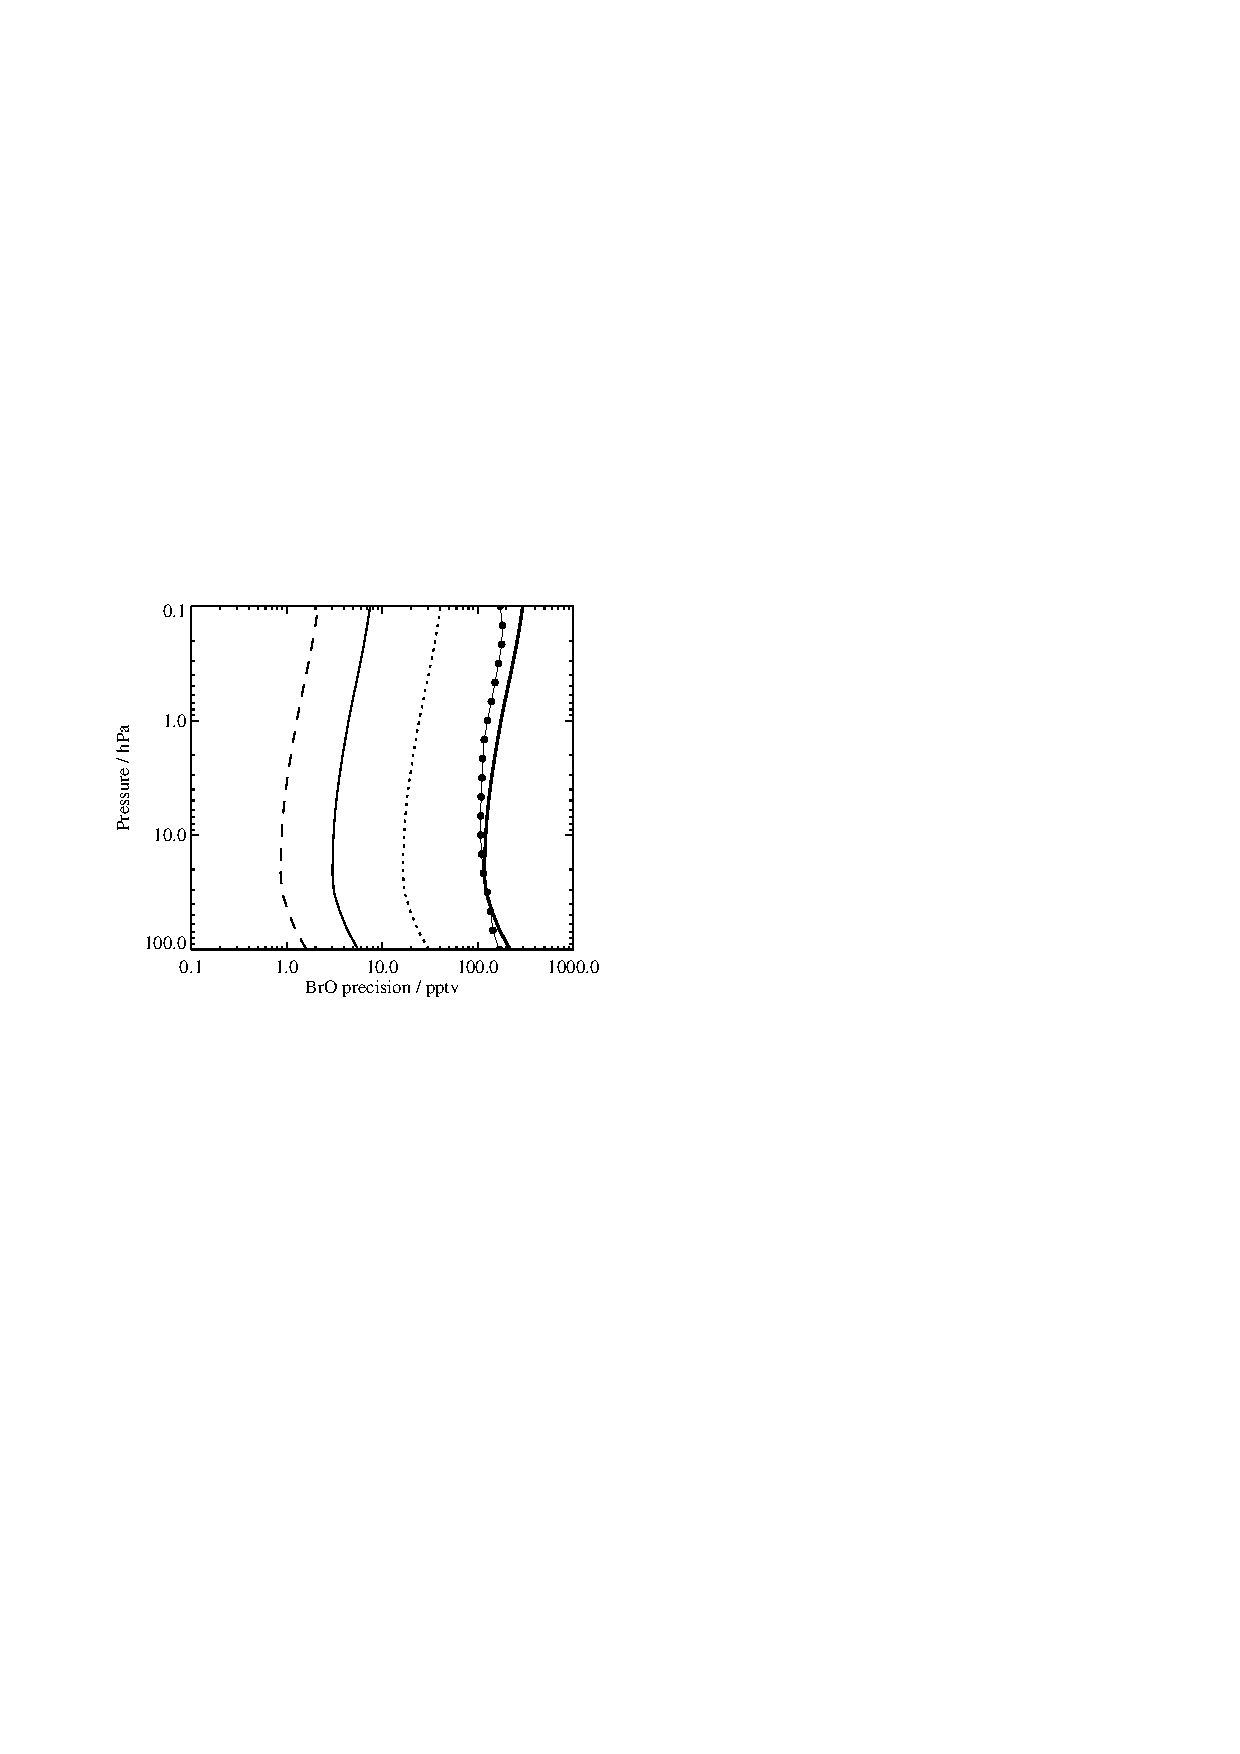
\includegraphics[width=0.4\linewidth]{figures/bro-precision}
\end{center}
\caption{Comparison of the MLS \thisv\CheckThis BrO precision as estimated from
  scatter in the retrieved data (circles) with that expected from the
  retrieval (thick line), for a single profile.  Also shown is the
  expected precision for the day/night difference of 10\degsym\ zonal
  mean profiles averaged over a day (dotted line), a month (thin line)
  and a year (dashed line).}
\label{fig:BrOPrecision}
\end{figure}

The expected precision in a retrieved profile is calculated from
radiance noise and reported for each retrieved data point.  The value of
the expected precision is flagged negative or zero if it is worse than
50\% of the value of the a priori precision.
Figure~\ref{fig:BrOPrecision} compares the expected precision (thick
line) on an individual MLS BrO measurement with that deduced from
observations of scatter in night-time observations (expected to be
zero). Also shown are the expected precisions for daily, monthly, and
yearly 10\degsym\ zonal means. For the minimal averaging recommended, a
monthly 10\degsym\ zonal mean, which corresponds to about 3,000
measurements, the precision is about $\pm$4\,ppt. See
Table~\ref{tab:BrOSummary} for more details.

\subsection{Accuracy}

The accuracy of the MLS BrO product is summarized in
Table~\ref{tab:BrOSummary}. The effect of each identified source of
systematic error on MLS measurements of radiance has been quantified and
modeled \citep{ReadEtal:2007}. These quantified effects correspond to
either $2\sigma$ estimates of uncertainties in each MLS product, or an
estimate of the maximum reasonable uncertainty based on instrument
knowledge and/or design requirements. More discussion is given in
\cite{KovalenkoEtal:2007:BrO}.  While that paper described v2.2 BrO, findings
are expected to be applicable also to \thisv\CheckThis. The potential systematic
bias in MLS BrO measurements can be as high as about $\pm$43\,ppt at
10\,hPa, decreasing to about $\pm$12\,pptv at 3.2\,hPa. The systematic
bias is dramatically reduced by subtracting the nighttime signal from
the daytime signal.  Taking the day/night difference reduces the
systematic biases to $\pm$16\,pptv at 10\,hPa and to $\pm$9\,pptv at
3.2\,hPa.  If the MLS BrO data is used at 3.2 hPa, the day/night
difference value will need to be adjusted to compensate for the
non-negligible nighttime BrO. We note that this method of taking
day/night differences is not applicable for polar summer and winter
during periods of continuous sunlight or darkness.

\subsection{Data screening}
\label{sec:BrOScreening}
\begin{description}
\item[Pressure range:] \screeningrule{10--3.2 hPa} \standardrangestatement
\item[Averaging required:] \screeningrule{Significant averaging (such as
    monthly zonal means) is required if useful scientific data are
    sought.}
\item[Diurnal differences:] \screeningrule{For use in any scientific
    study, day / night or ascending / descending differences should be used
    to alleviate biases.}  Note that, for 3.2\,hPa, the non-zero
  nighttime expected abundances BrO needs to be taken into account.
  \standardprecisionrule \evenstatusrule
\item[Clouds:] \cloudsokrule
\item[Quality:] \qualityrule{1.3}
\item[Convergence:] \convergencerule{1.05}
\end{description}

\subsection{Artifacts}
Significant biases exist in the BrO data, as discussed above. Day /
night (or ascending / descending) differences must be used to reduce
these.  For 3.2 hPa, nighttime BrO needs to be taken into account
\citep{KovalenkoEtal:2007:BrO}.

A systematic horizontal (i.e., profile-to-profile) oscillation has been
discovered in MLS \thisv\CheckThis (and earlier) standard BrO product.  This
presents a significant challenge to the interpretation of the BrO
observations.  Users are strongly advised to contact the MLS team before
embarking on research involving the MLS standard BrO product.  As
described above, use of other BrO products is preferable to using the
Level~2 BrO data.

\subsection{Review of comparisons with other data sets}
We have calculated total bromine, Br$_{y}$, from MLS measurements of BrO
using a photochemical model, and compared this with Br$_{y}$ similarly
inferred from balloon-borne measurements of BrO; good agreement is seen
\citep{KovalenkoEtal:2007:BrO}.


\begin{table}
\caption{Summary of the Aura MLS \thisv\CheckThis BrO product.}
% \caption{Summary of the Aura MLS BrO product.}
\vspace{\tablecaptionsep}
\label{tab:BrOSummary}
\begin{minipage}{\linewidth}
\centering\begin{tabular}{ccccl}
\toprule
\parbox[m]{5em}{\bfseries\centering Pressure range} &
\parbox[m]{4em}{\bfseries\centering Vertical res. / km} &
\parbox[m]{5.0em}{\bfseries\centering Precision\footnote{The precision quoted is for a 10\degsym\
    monthly zonal mean} / pptv} &
\parbox[m]{5.0em}{\bfseries\centering Day/night difference accuracy\footnote{Because of large biases in
    the data, the daytime and nighttime BrO data are unsuitable for
    scientific use, so day/night differences must be used. Note that
    day/night differences are not useful for polar winter and summer,
     where BrO does not undergo a diurnal variation.} / pptv} &
\textbf{Comments} \\
\midrule
%
2.2\,hPa and less & -- & -- & -- & Unsuitable for scientific use
  \\ %\addlinespace[2ex]
%
3.2\,hPa & 6 & $\pm$5 &$\pm$8
& \parbox[m]{10em}{\raggedright Need to
account for non-negligible night time BrO} \\ \addlinespace[2ex]

%
4.6 & 5.5 & $\pm$4 & $\pm$10  \\
6.8 & 5.5 & $\pm$4 & $\pm$11 \\ 
10  & 5.5 & $\pm$4 & $\pm$13 \\ 
150--15\,hPa   & -- & -- & -- & Unsuitable for scientific use \\
1000--215\,hPa & -- & -- & -- & Not retrieved \\
\bottomrule
\end{tabular}
\end{minipage}
\end{table}







%%% Local Variables: 
%%% mode: latex
%%% TeX-master: "v5-x-report"
%%% End: 

\speciestitle{Methyl chloride}{CH\cs3Cl}{CH3Cl}%
\begin{description}
\item[Useful range:] 147\,--\,4.6\,hPa
\item[Contact:] Michelle Santee, \email{Michelle.L.Santee@jpl.nasa.gov}
\end{description}
\label{sec:StandardCH3Cl}

\subsection*{Introduction}

The v2.2 MLS ClO measurements were characterized by a substantial
(\texttildelow0.1\,--\,0.4\,ppbv) negative bias at retrieval levels below (i.e.,
pressures larger than) 22\,hPa.  \citet{SanteeEtal08clo} suggested that
contamination from an interfering species such as CH\cs3Cl, which has
lines in two wing channels of the \mbox{640-GHz} band used to measure
ClO, could have given rise to the bias; they showed results from early
v3 algorithms in which CH\cs3Cl was also retrieved that demonstrated
significant reduction in the bias in lower stratospheric ClO\@.  Further
refinements in the \thisv algorithms yielded not only an improved ClO
product, but also a reliable retrieval of CH\cs3Cl.

As for ClO, the standard CH\cs3Cl product is derived from radiances
measured by the radiometer centered near 640\,GHz. The MLS \thisv CH\cs3Cl
data are scientifically useful over the range 147 to 4.6\,hPa.  A summary
of the precision and resolution (vertical and horizontal) of the \thisv
CH\cs3Cl measurements as a function of altitude is given in
Table~\ref{tab:CH3ClSummary}.  More details on the quality of the MLS
\thisv CH\cs3Cl measurements are given below.

\subsection*{Resolution}
\onestandardavk{CH3Cl}{CH\cs3Cl}%

The resolution of the retrieved data can be described using ``averaging
kernels'' \citep[e.g.,][]{Rodgers00}; the two-dimensional nature of the
MLS data processing system means that the kernels describe both vertical
and horizontal resolution.  Smoothing, imposed on the retrieval system
in both the vertical and horizontal directions to enhance retrieval
stability and precision, degrades the inherent resolution of the
measurements.  Consequently, the vertical resolution of the \thisv
CH\cs3Cl data, as determined from the full width at half maximum of the
rows of the averaging kernel matrix shown in Figure~\ref{fig:AvkCH3Cl},
is \texttildelow4\,--\,6\,km in most of the lower stratosphere, degrading to
7\,--\,10\,km at and above (i.e., at pressures less than) 14\,hPa.  Note
that there is overlap in the averaging kernels for the 100 and 147\,hPa
retrieval surfaces, indicating that the 147\,hPa retrieval does not
provide as much independent information as is given by retrievals at
higher altitudes.  Figure~\ref{fig:AvkCH3Cl} also shows horizontal
averaging kernels, from which the along-track horizontal resolution is
determined to be \texttildelow600\,km at 147\,hPa, \texttildelow450\,--\,500\,km from
100 to 22\,hPa, and \texttildelow550\,--\,850\,km at and above 15\,hPa.  The
cross-track resolution, set by the width of the field of view of the
\mbox{640-GHz} radiometer, is \texttildelow3\,km.  The along-track separation
between adjacent retrieved profiles is 1.5\degsym\ great circle angle
(\texttildelow165\,km), whereas the longitudinal separation of MLS
measurements, set by the Aura orbit, is 10\degsym--\,20\degsym\ over low
and middle latitudes, with much finer sampling in the polar regions.

\subsection*{Precision}

\begin{figure}
\centering\dontincludegraphics[width=12.0cm]{figures/MLSCH3Clascdsc-200502}
\caption{(left) Ensemble mean profiles for ascending (red) and
  descending (blue) orbit matching pairs of MLS \thisv CH\cs3Cl in the
  latitude range 50\degsym S\,--\,50\degsym N averaged over 30 days in April
  2008.  (right) Mean difference profiles between ascending and
  descending orbits (cyan), the standard deviation about the mean
  difference (orange), and the root sum square of the precisions
  calculated by the retrieval algorithm (magenta).  SD values are scaled
  by 1/$\sqrt{2}$; thus the observed SD represents the statistical
  repeatability of the MLS measurements, and the expected SD represents
  the theoretical \mbox{1-$\sigma$} precision for a single profile.  See
  \citet{LambertEtal07} for details.  }
\label{fig:CH3Clascdsc}
\end{figure}

The precision of the MLS CH\cs3Cl data is estimated empirically by
computing the standard deviation of the differences between matched
measurement points at the intersections of the ascending (day) and
descending (night) sides of the orbit.  Observed scatter, representing
the statistical repeatability of the measurements, is 100\,pptv or less
throughout the vertical domain.  This estimate reflects the precision of
a single profile; in most cases precision can be improved by averaging,
with the precision of an average of $N$ profiles being 1/$\sqrt{N}$
times the precision of an individual profile (note that this is not the
case for averages of successive along-track profiles, which are not
completely independent because of horizontal smearing).  The theoretical
precision reported by the Level~2 data processing system exceeds the
observationally-determined precision throughout the vertical range,
indicating that the smoothing applied to stabilize the retrieval and
improve the precision has a nonnegligible influence.  Because the
theoretical precisions take into account occasional variations in
instrument performance, the best estimate of the precision of an
individual data point is the value quoted for that point in the L2GP
files, but it should be borne in mind that this approach slightly
overestimates the actual measurement noise.

\subsection*{Range}

Although CH\cs3Cl is retrieved (and reported in the L2GP files) over the
range 147 to 0.001\,hPa, on the basis of the drop off in precision and
resolution, the reduction in independent information contributed by the
measurements, and the results of simulations using synthetic data as
input radiances to test the closure of the retrieval system, the data
are not deemed reliable at retrieval levels above (i.e., pressures lower
than) 4.6\,hPa.  Despite the overlap in the averaging kernels for the
147 and 100\,hPa surfaces (Figure~\ref{fig:AvkCH3Cl}), maps at 147\,hPa
display substantial features not seen at 100\,hPa (not shown) that are
believed to represent real atmospheric variations.  Thus we recommend
that the \thisv CH\cs3Cl data may be used for scientific studies between
147 and 4.6\,hPa, inclusive.

\subsection*{Accuracy}

The impact of various sources of systematic uncertainty has not yet been
quantified for CH\cs3Cl as it has for most other MLS products.  This
work is planned as part of a dedicated validation exercise for the \thisv
CH\cs3Cl data.

\subsection*{Review of comparisons with other datasets}

Detailed comparisons with correlative data sets have not yet been
undertaken.  This work is planned as part of a dedicated validation
exercise for the \thisv CH\cs3Cl data.

\subsection*{Data screening}
\begin{description}
\item[Pressure range:]  \screeningrule{147\,--\,4.6\,hPa}

  \standardrangestatement
  
  \standardprecisionrule
  
\item[Status flag:] \screeningrule{Only use profiles for which the
    `Status' field is zero.}  We recommend that all profiles with
  nonzero values of `Status' be discarded, because of the potential
  impact of cloud artifacts at lower levels.  See
  Section~\ref{sec:StatusQuality} for more information on the
  interpretation of the \texttt{Status} field.

\item[Clouds:] \cloudsokrule

  Nonzero but even values of \texttt{Status} indicate that the profile
  has been marked as questionable, usually because the measurements may
  have been affected by the presence of thick clouds.  Globally fewer
  than \texttildelow1\,--\,2\% of CH\cs3Cl profiles are typically identified in
  this manner (though this value rises to \texttildelow3\,--\,5\% in the
  tropics on a typical day), and cloud artifacts may be especially
  prevalent at 147\,hPa.

\item[Quality:] \qualityrule{1.3}

  This threshold for \texttt{Quality} (see
  section~\ref{sec:StatusQuality}) typically excludes less than 1\% of
  CH\cs3Cl profiles on a daily basis; note that it potentially discards
  some ``good'' data points while not necessarily identifying all
  ``bad'' ones.

\item[Convergence:] \convergencerule{1.05}

  On a typical day this threshold for \texttt{Convergence} (see
  Section~\ref{sec:StatusQuality}) discards very few (0.3\% or less) of
  the CH\cs3Cl profiles, most (but not all) of which are also filtered
  out by the other quality control measures.
\end{description}

\subsection*{Artifacts}

\begin{itemize}
\item To be determined.
\end{itemize}

\subsection*{Desired improvements for future data version(s)}

\begin{itemize}
\item To be determined.
\end{itemize}

\begin{table*}[bp]
\caption{Summary of Aura MLS \thisv CH\cs3Cl Characteristics}\vspace{0.5ex}
\label{tab:CH3ClSummary}
\begin{minipage}{\linewidth}
\renewcommand{\thefootnote}{\thempfootnote}
\centering\begin{tabular}{ccccl}
\toprule
\parbox[m]{18mm}{\bfseries\centering{Pressure\\ / hPa}} &
\parbox[m]{24mm}{\bfseries\centering{Resolution\\ V $\times$ H%
\footnote{Vertical and Horizontal resolution in along-track direction.} \\ / km}} &
\parbox[m]{18mm}{\bfseries\centering{Precision%
    \footnote{Precision on individual profiles.} \\/ pptv}} &
\parbox[m]{20mm}{\bfseries\centering{Accuracy\\ / pptv}} &
\parbox[m]{40mm}{\bfseries\centering{Known Artifacts\\ or Other Comments}} \\
%
\midrule
%
3.2\,--\,0.001 & ---   & ---    & ---     & for scientific
  use\\
%
15\,--\,4.6  & 7\,--\,10 $\times$ 550\,--\,850 & $\pm$100 & TBD & \\
%
100\,--\,22  & 4\,--\,6 $\times$ 450\,--\,500 & $\pm$100 & TBD &  \\
%
147      & 4.5 $\times$ 600 & $\pm$100 & TBD & \\
%
1000\,--\,215  & ---    & ---     & ---     & retrieved\\
%
\bottomrule
\end{tabular}
\end{minipage}
\end{table*}

%%% Local Variables: 
%%% mode: latex
%%% TeX-master: "v4-x-report"
%%% End: 


\speciestitle{Methyl cyanide}{CH\cs3CN}{CH3CN}%
\begin{description}
\item[Useful range:] 46\,--\,1.0\,hPa
\item[Contact:] Michelle Santee, \email{Michelle.L.Santee@jpl.nasa.gov}
\end{description}
\label{sec:StandardCH3CN}%

\subsection*{Introduction}

The v2.2 standard CH\cs3CN data, which were derived from radiances
measured by the radiometer centered near 190\,GHz, were not recommended
for use in scientific studies.  In \thisv, the standard CH\cs3CN product
is taken from radiances measured by the radiometer centered near
640\,GHz.  In addition, the quality and reliability of the
\mbox{640-GHz} CH\cs3CN retrievals themselves have been improved in
\thisv, largely because of changes in the way that the continuum is being
handled for this radiometer in the v3 algorithms.  The MLS CH\cs3CN data
are now deemed scientifically useful over the range 46 to 1\,hPa, except
in the winter polar vortex regions, where they may exhibit large biases
below 10\,hPa.  In addition, the data at lower retrieval levels (i.e.,
higher pressures) may be used with caution in certain circumstances.  A
summary of the precision and resolution (vertical and horizontal) of the
\thisv CH\cs3CN measurements as a function of altitude is given in
Table~\ref{tab:CH3CNSummary}.  More details on the quality of the MLS
\thisv CH\cs3CN measurements are given below.

\subsection*{Resolution}
\onestandardavk{CH3CN}{CH\cs3CN}%

The resolution of the retrieved data can be described using ``averaging
kernels'' \citep[e.g.,][]{Rodgers00}; the two-dimensional nature of the
MLS data processing system means that the kernels describe both vertical
and horizontal resolution.  Smoothing, imposed on the retrieval system
in both the vertical and horizontal directions to enhance retrieval
stability and precision, degrades the inherent resolution of the
measurements.  Consequently, the vertical resolution of the \thisv
CH\cs3CN data, as determined from the full width at half maximum of the
rows of the averaging kernel matrix shown in Figure~\ref{fig:AvkCH3CN},
is \texttildelow5\,--\,6\,km in the lower stratosphere, degrading to
\texttildelow7\,--\,8\,km in the upper stratosphere.  Note that there is
overlap in the averaging kernels for the 100 and 147\,hPa retrieval
surfaces, indicating that the 147\,hPa retrieval does not provide as
much independent information as is given by retrievals at higher
altitudes.  Figure~\ref{fig:AvkCH3CN} also shows horizontal averaging
kernels, from which the along-track horizontal resolution is determined
to be \texttildelow400\,--\,700\,km over most of the vertical range.  The
cross-track resolution, set by the width of the field of view of the
\mbox{640-GHz} radiometer, is \texttildelow3\,km.  The along-track separation
between adjacent retrieved profiles is 1.5\degsym\ great circle angle
(\texttildelow165\,km), whereas the longitudinal separation of MLS
measurements, set by the Aura orbit, is 10\degsym--\,20\degsym\ over low
and middle latitudes, with much finer sampling in the polar regions.

\subsection*{Precision}

\begin{figure}
\centering\dontincludegraphics[width=14.0cm]{figures/CH3CN_ASCDSC_200804}
\caption{ (left) Ensemble mean profiles for ascending (red) and
  descending (blue) orbit matching pairs of MLS \thisv CH\cs3CN in the
  latitude range 50\degsym S\,--\,50\degsym N averaged over 30 days in April
  2008.  (center) Mean percent difference profiles between ascending and
  descending orbits (cyan), the standard deviation about the mean
  difference (orange), and the root sum square of the precisions
  calculated by the retrieval algorithm (magenta).  (right) Same, for
  absolute differences (pptv).  SD values are scaled by 1/$\sqrt{2}$;
  thus the observed SD represents the statistical repeatability of the
  MLS measurements, and the expected SD represents the theoretical
  \mbox{1-$\sigma$} precision for a single profile.  See
  \citet{LambertEtal07} for details.  }
\label{fig:ascdsc}
\end{figure}

The precision of the MLS CH\cs3CN data is estimated empirically by
computing the standard deviation of the differences between matched
measurement points at the intersections of the ascending (day) and
descending (night) sides of the orbit.  That the mean differences
between paired profiles are minimal (Figure~\ref{fig:ascdsc}) indicates
the absence of systematic ascending / descending biases.  Observed
scatter, representing the statistical repeatability of the measurements,
is 50\,--\,100\,pptv throughout the vertical domain.  This estimate reflects
the precision of a single profile; in most cases precision can be
improved by averaging, with the precision of an average of $N$ profiles
being 1/$\sqrt{N}$ times the precision of an individual profile (note
that this is not the case for averages of successive along-track
profiles, which are not completely independent because of horizontal
smearing).  The theoretical precision reported by the Level~2 data
processing system slightly exceeds the observationally-determined
precision throughout the vertical range, indicating that the smoothing
applied to stabilize the retrieval and improve the precision has a
nonnegligible influence.  Because the theoretical precisions take into
account occasional variations in instrument performance, the best
estimate of the precision of an individual data point is the value
quoted for that point in the L2GP files, but it should be borne in mind
that this approach slightly overestimates the actual measurement noise.

\subsection*{Range}

Although CH\cs3CN is retrieved (and reported in the L2GP files) over the
range 147 to 0.001\,hPa, on the basis of the drop off in precision and
resolution, the lack of independent information contributed by the
measurements, and the results of simulations using synthetic data as
input radiances to test the closure of the retrieval system, the data
are not deemed reliable at the extremes of the retrieval range.  Thus we
recommend that \thisv CH\cs3CN be used for scientific studies only at the
levels between 46 and 1\,hPa.  However, although the 147, 100, and
68\,hPa retrievals are not generally recommended, they may be
scientifically useful in some circumstances.  For example, the data
display unphysical sharp latitudinal gradients at $\pm$30\degsym\ at 100
and 68\,hPa, yet the large-scale longitudinal variations within the
tropics are probably robust.  Similarly, confined regions of significant
enhancement at 147\,hPa unaccompanied by comparably enhanced values at
100\,hPa may reflect real atmospheric features.  The \thisv CH\cs3CN data
at these levels (147\,--\,68\,hPa) should only be used in consultation with
the MLS science team.

\subsection*{Accuracy}

\begin{figure}
\centering
\dontincludegraphics[width=8.0cm]{figures/ch3cn_zonalmean_livesey2000}
\hspace{2em}
\parbox[b]{6cm}{%
\dontincludegraphics[width=5.8cm]{figures/Zm_CH3CN_v03-3x__2007d001-2007d031}\\
\dontincludegraphics[width=5.8cm]{figures/Zm_CH3CN_v03-3x__2007d182-2007d212}}
\caption{(left plot) Top row shows UARS MLS mean CH\cs3CN fields for
  June / July 1993 (left) and December 1992 / January 1993 (right).  The
  other rows show results from various chemistry transport model runs.
  See \citet{LiveseyEtal01} for details. (right plot) \thisv Aura MLS
  CH\cs3CN monthly zonal means for January (top) and July (bottom)
  2007. }
\label{fig:ch3cnZM}
\end{figure}

The impact of various sources of systematic uncertainty has not yet been
quantified for CH\cs3CN as it has for most other MLS products.  This
work is planned as part of a dedicated validation exercise for the \thisv
CH\cs3CN data.  However, preliminary comparisons with results from a
two-dimensional chemistry transport model and CH\cs3CN retrievals from
the MLS instrument on the Upper Atmosphere Research Satellite (UARS)
\citep{LiveseyEtal01} indicate that the \thisv Aura MLS CH\cs3CN mixing
ratios are biased substantially high in the lower stratosphere
(147\,--\,68\,hPa, see Figure~\ref{fig:ch3cnZM}).  Furthermore, the
zonal-mean morphology of the Aura MLS CH\cs3CN at the lowest levels does
not agree well with that either observed by UARS MLS or predicted by the
model.

\subsection*{Review of comparisons with other datasets}

Detailed comparisons with correlative data sets have not yet been
undertaken.  This work is planned as part of a dedicated validation
exercise for the \thisv CH\cs3CN data.

\subsection*{Data screening}
\begin{description}
\item[Pressure range:] \screeningrule{46\,--\,1.0\,hPa}
    \standardrangestatement\ The CH\cs3CN data at 147\,--\,68\,hPa may be
    useful under certain circumstances but should not be analyzed in
    scientific studies without significant discussion with the MLS
    science team.

\standardprecisionrule

\evenstatusrule

\item[Clouds:] \cloudsokrule

  Nonzero but even values of \texttt{Status} indicate that the profile
  has been marked as questionable, usually because the measurements may
  have been affected by the presence of thick clouds.  Globally fewer
  than \texttildelow1\,--\,2\% of CH\cs3CN profiles are typically identified in
  this manner (though this value rises to \texttildelow3\,--\,5\% in the tropics on
  a typical day), and clouds generally have little influence on the
  stratospheric CH\cs3CN data.  Thus profiles with even values of
  \texttt{Status} may be used without restriction.

\item[Quality:] \qualityrule{1.4}

  This threshold for \texttt{Quality} (see
  section~\ref{sec:StatusQuality}) typically excludes less than 1\% of
  CH\cs3CN profiles on a daily basis; note that it potentially discards
  some ``good'' data points while not necessarily identifying all
  ``bad'' ones.
\item[Convergence:] \convergencerule{1.05}

  On a typical day this threshold for \texttt{Convergence} (see
  section~\ref{sec:StatusQuality}) discards very few (0.3\% or less) of
  the CH\cs3CN profiles, many (but not all) of which are filtered out by
  the other quality control measures.
\end{description}

\subsection*{Artifacts}
\begin{itemize}
\item The retrievals at 100 and 68\,hPa are characterized by unphysical
  sharp latitudinal gradients at $\pm$30\degsym.
\item Substantial biases may be present in the mixing ratios in the
  winter polar vortex regions for retrieval levels in the range
  100\,--\,15\,hPa.
\end{itemize}

\subsection*{Desired improvements for future data version(s)}
\begin{itemize}
\item Improve the CH\cs3CN retrievals at 147\,--\,68\,hPa.
\end{itemize}

\begin{table*}[bp]
\caption{Summary of Aura MLS \thisv CH\cs3CN Characteristics}\vspace{0.5ex}
\label{tab:CH3CNSummary}
\begin{minipage}{\linewidth}
\renewcommand{\thefootnote}{\thempfootnote}
\centering\begin{tabular}{ccccl}
\toprule
\parbox[m]{18mm}{\bfseries\centering{Pressure\\ / hPa}} &
\parbox[m]{24mm}{\bfseries\centering{Resolution\\ V $\times$ H%
\footnote{Vertical and Horizontal resolution in along-track direction.} \\ / km}} &
\parbox[m]{18mm}{\bfseries\centering{Precision%
    \footnote{Precision on individual profiles.} \\/ pptv}} &
\parbox[m]{20mm}{\bfseries\centering{Accuracy\\ / pptv}} &
\parbox[m]{40mm}{\bfseries\centering{Known Artifacts\\ or Other Comments}} \\
%
\midrule
%
0.68\,--\,0.001 & ---   & ---    & ---     & Unsuitable for scientific
  use\\
%
1.0      & 6 $\times$ 800 & $\pm$100 & TBD & \\
%
46\,--\,1.5  & 5\,--\,8 $\times$ 400\,--\,700 & $\pm$50 & TBD & \\
%
100\,--\,68  & 5\,--\,6 $\times$ 600\,--\,700 & $\pm$50 & TBD & Consult with
MLS science team \\
%
147      & 4 $\times$ 800        & $\pm$100 & TBD & Consult with
MLS science team \\
%
1000\,--\,215  & ---    & ---     & ---      & Not retrieved\\
%
\bottomrule
\end{tabular}
\end{minipage}
\end{table*}

%%% Local Variables: 
%%% mode: latex
%%% TeX-master: "v4-x-report"
%%% End: 

\speciestitle{Methanol}{CH\cs3OH}{CH3OH}%
{\item[Useful range:] 147\,--\,100\,hPa
\item[Contact:] Michelle Santee, \email{Michelle.L.Santee@jpl.nasa.gov}}
\label{sec:StandardCH3OH}%

\newcommand{\meoh}{CH\cs3OH\xspace}

\subsection*{Introduction}

The standard CH\cs3OH product is taken from radiances measured by the
radiometer centered near 640\,GHz.  CH\cs3OH is a new product in
\thisv, and it has not yet been fully validated.  Thus the scientific
utility of the \thisv MLS CH\cs3OH measurements remains to be
determined.

\subsection*{Resolution}
\onestandardavk{CH3OH}{CH\cs3OH}%

The resolution of the retrieved data can be described using
``averaging kernels'' \citep[e.g.,][]{Rodgers00}; the two-dimensional
nature of the MLS data processing system means that the kernels
describe both vertical and horizontal resolution.  Values of the
integrated kernel near unity indicate that the majority of information
for that level has come from the measurements themselves and not the a
priori; Figure~\ref{fig:AvkCH3OH} shows that the measurements dominate
throughout most of the vertical range. Smoothing, imposed on the
retrieval system in both the vertical and horizontal directions to
enhance retrieval stability and precision, degrades the inherent
resolution of the measurements.  Thus, although CH\cs3OH measurements
are reported at six pressure levels per decade change in pressure
(spacing of \texttildelow2.7\,km), the vertical resolution of the
\thisv CH\cs3OH data as determined from the full width at half maximum
of the rows of the averaging kernel matrix shown in
Figure~\ref{fig:AvkCH3OH} is \texttildelow4--5\,km at 147 and
100\,hPa.  Figure~\ref{fig:AvkCH3OH} also shows horizontal averaging
kernels, from which the along-track horizontal resolution is
determined to be \texttildelow350\,km.  The cross-track resolution,
set by the width of the field of view of the \mbox{640-GHz}
radiometer, is \texttildelow3\,km.  The along-track separation
between adjacent retrieved profiles is 1.5\degsym\ great circle angle
(\texttildelow165\,km), whereas the longitudinal separation of MLS
measurements, set by the Aura orbit, is 10\degsym--\,20\degsym\ over
low and middle latitudes, with much finer sampling in the polar
regions.

\subsection*{Precision}

\begin{figure}
\centering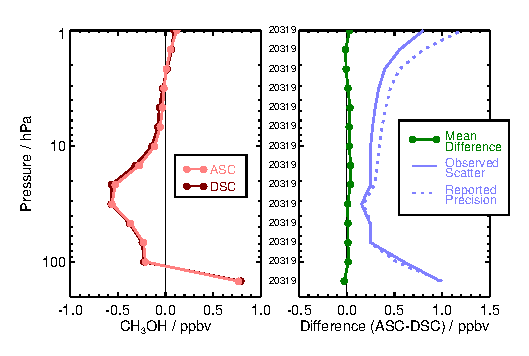
\includegraphics[width=10.0cm]{figures/MLSascdsc_CH3OH_clim}
\caption{(left) Ensemble mean profiles for ascending (light red) and
  descending (dark red) orbit matching pairs of MLS \thisv CH\cs3OH
  profiles averaged over several months of a representative year of
  data (2005).  Symbols indicate MLS retrieval pressure levels.
  (right) Mean differences (ascending$-$descending) in pptv (green
  solid line).  Also shown are the standard deviations about the mean
  differences (light blue solid line) and the root sum square (RSS) of
  the precisions calculated by the retrieval algorithm for the two
  sets of profiles (light blue dashed line). The observed scatter
  about the mean differences and the reported precision values have
  been scaled by 1/$\sqrt{2}$ (to convert from standard deviations of
  differences into standard deviations of individual data points);
  hence the light blue solid line represents the statistical
  repeatability of the MLS measurements, and the light blue dashed
  line represents the expected \mbox{1-$\sigma$} precision for a
  single profile.  The thin black lines mark zero in each panel.  The
  number of crossing pairs of measurements being compared at each
  pressure level is noted in the space between the panels.}
\label{fig:mlsascdscCH3OH}
\end{figure}

The precision of the MLS CH\cs3OH data is estimated empirically by
comparing profiles measured at the intersections of ascending (day)
and descending (night) portions of the orbit. Under ideal conditions
(i.e., a quiescent atmosphere), the standard deviation about the mean
differences between such matched profile pairs provides a measure of
the precision of the individual data points. In practice, however,
real changes in the atmosphere may occur over the 12\,h interval
between the intersecting measurement points, in which case the
observed scatter provides an upper limit on the estimate of precision,
assuming that the a priori has a negligible influence on the retrieval
(a reasonable assumption throughout the retrieval range for
CH\cs3OH). The precision estimates were found to be essentially
invariant with time; results for several months of a representative
year of data are shown in Figure~\ref{fig:mlsascdscCH3OH}.  For the
most part, differences between paired profiles are small, implying the
absence of significant systematic ascending / descending biases. The
observed standard deviation is \texttildelow1\,ppbv at 147\,hPa. The
observationally determined precision agrees well with that reported
for each data point by the Level~2 data processing system.  The
estimates reported here represent the precisions at each pressure
level of a single profile; precision can generally be improved by
averaging, with the precision of an average of $N$ profiles being
1/$\sqrt{N}$ times the precision of an individual profile (although
the actual standard error of the mean can in some cases be even
smaller \citep{TooheyAndVonClarmann13}).

\subsection*{Range}

CH\cs3OH is retrieved (and reported in the Level~2 files) over the
range 147 to 0.001\,hPa.  However, zonal mean mixing ratios are
negative everywhere at retrieval pressures less than 100\,hPa, as well
as at middle and high latitudes at 100\,hPa.  Thus, with rare
exceptions (such as during extreme events), the v4 \meoh\ data are
considered potentially useful for scientific studies only at 147\,hPa
and at lower latitudes at 100\,hPa.

\subsection*{Accuracy}

The impact of various sources of systematic uncertainty has not yet
been quantified for CH\cs3OH as it has for most other MLS products.
This work is planned as part of a dedicated validation exercise for
the \thisv CH\cs3OH data.

\subsection*{Review of comparisons with other datasets}

Detailed comparisons with correlative data sets have not yet been
undertaken.  This work is planned as part of a dedicated validation
exercise for the \thisv CH\cs3OH data.

\subsection*{Data screening}
\begin{description}
\item[Do not use:] Until more comprehensive validation studies have
  been done, the \thisv CH\cs3OH data should only be used in
  consultation with the MLS science team.
\end{description}

\subsection*{Artifacts}
\begin{itemize}
\item A complete assessment of artifacts in the \thisv CH\cs3OH
  measurements has not yet been performed, but it is known that zonal
  mean mixing ratios are negative everywhere at retrieval pressures
  less than 100\,hPa, as well as at middle and high latitudes at
  100\,hPa.
\end{itemize}

\subsection*{Desired improvements for future data version(s)}
\begin{itemize}
\item Specific improvements in the CH\cs3OH retrieval remain to be
  determined.
\end{itemize}

\begin{table*}[bp]
\caption{Summary of Aura MLS \thisv CH\cs3OH Characteristics}\vspace{0.5ex}
\label{tab:CH3OHSummary}
\begin{minipage}{\linewidth}
\renewcommand{\thefootnote}{\thempfootnote}
\centering\begin{tabular}{ccccl}
\toprule
\parbox[m]{18mm}{\bfseries\centering{Pressure\\ / hPa}} &
\parbox[m]{24mm}{\bfseries\centering{Resolution\\ V $\times$ H%
\footnote{Vertical and Horizontal resolution in along-track direction.} \\ / km}} &
\parbox[m]{18mm}{\bfseries\centering{Precision%
    \footnote{Precision on individual profiles.} \\/ ppbv}} &
\parbox[m]{20mm}{\bfseries\centering{Accuracy\\ / ppbv}} &
\parbox[m]{40mm}{\bfseries\centering{Known Artifacts\\ or Other Comments}} \\
%
\midrule
%
68\,--\,0.001  & ---                             & ---      & ---  & Unsuitable for scientific use\\
%
100            & 5         $\times$ 350          & $\pm$1   & TBD  &  \\
%
147            & 4         $\times$ 150          & $\pm$1   & TBD  & \\
%
1000\,--\,215  & ---                             & ---      & ---  & Not retrieved\\
%
\bottomrule
\end{tabular}
\end{minipage}
\end{table*}

%%% Local Variables: 
%%% mode: latex
%%% TeX-master: "v4-x-report"
%%% End: 

\speciestitle{Chlorine Monoxide}{ClO}{ClO}{%
\item[Useful range:] 147--1.0\,hPa
\item[Contact:] Michelle Santee, \email{Michelle.L.Santee@jpl.nasa.gov}}

\subsection{Introduction}

As in previous versions, in \thisv the standard ClO product is derived
from radiances measured by the radiometer centered near 640\,GHz.  ClO
is also retrieved using radiances from the \mbox{190-GHz} radiometer,
but those data have poorer precision and larger biases and are not
used in the standard ClO product.  The quality and reliability of the
version~2 (v2.2) Aura MLS ClO measurements were assessed in detail by
\citet{SanteeEtal:2008:ClO}.  The ClO product was significantly
improved in v3.3\emph{x}/v3.4\emph{x} \citep{EOSMLSV33V34Quality}; in
particular, the substantial (\mytexttilde0.1--0.4\,ppbv) negative
bias present in the v2.2 ClO values at retrieval levels below (i.e.,
pressures larger than) 22\,hPa was mitigated to a large extent,
primarily through retrieval of CH\cs3Cl, which was a new MLS product
in v3.3\emph{x}/v3.4\emph{x}.  The ClO retrieval was largely unchanged
over much of the profile in \prevv, and the \thisv retrieval does not
depart dramatically from \prevv, although the biases present at the
lowest retrieval levels have been further reduced (see
Section~\ref{sec:cloBias}).  The MLS \thisv ClO data are
scientifically useful over the range 147 to 1\,hPa.  A summary of the
estimated precision, resolution (vertical and horizontal), and
systematic uncertainty of the \thisv ClO measurements as a function of
altitude is given in Table~\ref{tab:ClOSummary}.

\subsection{Resolution}
\onestandardavk{ClO}{ClO}%

The resolution of the retrieved data can be described using
``averaging kernels'' \citep[e.g.,][]{Rodgers:2000}; the
two-dimensional nature of the MLS data processing system means that
the kernels describe both vertical and horizontal resolution.
Smoothing, imposed on the retrieval system in both the vertical and
horizontal directions to enhance retrieval stability and precision,
degrades the inherent resolution of the measurements.  Thus, although
ClO measurements are reported at six pressure levels per decade change
in pressure (spacing of \mytexttilde2.7\,km), the vertical resolution
of the \thisv ClO data as determined from the full width at half
maximum of the rows of the averaging kernel matrix shown in
Figure~\ref{fig:AvkClO} is \mytexttilde3--4.5\,km throughout the
retrieval range (with a mean of \mytexttilde3.5\,km).  As in \prevv,
in \thisv the averaging kernels are sharply peaked at all levels,
including 147\,hPa.  Thus, although some degree of overlap is present,
the 147\,hPa surface provides independent information in \thisv.
Figure~\ref{fig:AvkClO} also shows horizontal averaging kernels, from
which the along-track horizontal resolution is determined to be
\mytexttilde300--500\,km over most of the vertical range.  The
cross-track resolution, set by the width of the field of view of the
\mbox{640-GHz} radiometer, is \mytexttilde3\,km.  The along-track
separation between adjacent retrieved profiles is 1.5{\degsym} great
circle angle (\mytexttilde165\,km), whereas the longitudinal
separation of MLS measurements, set by the Aura orbit, is
10{\degsym}--20{\degsym} over low and middle latitudes, with much
finer sampling in the polar regions.

\subsection{Precision}

\begin{figure}
\centering\includegraphics[width=8.4cm]{figures/ComparePrecision2Panel-ClO}
\caption{Precision of the (left) \thisv and (right) \prevv MLS ClO
  measurements for four representative days in different seasons (see
  legend).  Solid lines depict the observed scatter in nighttime
  (descending) measurements obtained in a narrow equatorial band (see
  text); dotted lines depict the theoretical precision estimated by
  the retrieval algorithm. The light grey vertical line marks
  0.1\,ppbv, the estimated single-profile precision over most of the
  recommended vertical range in both versions.}
\label{fig:ClOPrecProf}
\end{figure}

The precision of the MLS ClO measurements is estimated empirically by
computing the standard deviation of the descending (i.e., nighttime)
profiles in the 20{\degsym}-wide latitude band centered around the
equator.  For this region and time of day, natural atmospheric
variability should be negligible relative to the measurement noise.
As shown in Figure~\ref{fig:ClOPrecProf}, the observed scatter in the
data is virtually unchanged in \thisv, ranging from
\mytexttilde0.1\,ppbv over the interval 100--3\,hPa to
\mytexttilde0.2\,ppbv at 147\,hPa and \mytexttilde0.3\,ppbv at
1\,hPa.  The smoothing of the retrieval is turned off above 1\,hPa,
and as a consequence the precision worsens steeply above this level.
The scatter in the data is essentially invariant with time, as seen by
comparing the results for the different days shown in
Figure~\ref{fig:ClOPrecProf}.

The single-profile precision estimates cited here are, to first order,
independent of latitude and season, but of course the scientific
utility of individual MLS profiles (i.e., signal to noise) varies with
ClO abundance.  Outside of the lower stratospheric winter polar
vortices, within which ClO is often strongly enhanced, the
single-profile precision exceeds typical ClO mixing ratios,
necessitating the use of averages for scientific studies.  Precision
can generally be improved by averaging, with the precision of an
average of $N$ profiles being 1/$\sqrt{N}$ times the precision of an
individual profile (although the actual standard error of the mean can
in some cases be even smaller \citep{TooheyAndVonClarmann:2013}).

The observational determination of the precision is compared in
Figure~\ref{fig:ClOPrecProf} to the theoretical precision values
reported by the Level~2 data processing algorithms.  The predicted
precision exceeds the observed scatter, particularly above 15\,hPa,
indicating that the vertical smoothing (regularization) applied to
stabilize the retrieval and improve the precision has a non-negligible
influence on the results at these levels.  Because the theoretical
precisions take into account occasional variations in instrument
performance, the best estimate of the precision of an individual data
point is the value quoted for that point in the L2GP files, but it
should be borne in mind that this approach slightly overestimates the
actual measurement noise.

\subsection{Accuracy}
\label{sec:cloacc}

The effects of various sources of systematic uncertainty (e.g.,
instrumental issues, spectroscopic uncertainty, and approximations in
the retrieval formulation and implementation) on the MLS \thisv ClO
measurements have been quantified through a comprehensive set of
retrievals of synthetic radiances; see \citet{SanteeEtal:2008:ClO} for
details of a similar analysis conducted on MLS v2.2 ClO data.  The
overall systematic uncertainty, or accuracy, is calculated by
combining (RSS) the contributions from both the expected biases and
the additional scatter each source of uncertainty may introduce into
the data.  In aggregate, the factors considered in these simulations
are estimated to give rise to a total systematic uncertainty ranging
from approximately 0.02 to 0.6\,ppbv, depending on the level, in the
MLS \thisv ClO data (see Table~\ref{tab:ClOSummary}).  These values
for the overall uncertainty in \thisv ClO, which are slightly larger
(poorer accuracy) at 100 and 147\,hPa than those estimated for the
\prevv data \citep[see][]{EOSMLSV4Quality}, do not take into account
the known biases in MLS ClO data at the lowest retrieval levels
discussed in the following subsection.

\subsection{Quantification and correction of biases in
  \prevv and \thisv}
\label{sec:cloBias}

As with other species retrieved from the MLS \mbox{640-GHz} receiver,
lower stratospheric signals for ClO are affected by water
vapor. Therefore, for the retrieval phase CorePlusR4AB14, which
includes ClO (see Table~\ref{tab:Phases}), water vapor is constrained
to the values from the MLS H\cs2O standard product.  As discussed in
Section~\ref{sec:H2OChanges}, the dry bias below the tropopause
present in earlier MLS data versions has been mitigated in \thisv.
Some of the differences between \thisv and \prevv ClO can thus be
attributed to the improvement in H\cs2O between the two versions.
Zonal-mean differences from \prevv are generally small (less than
10\%) except at the bottom of the retrieval range (68--147\,hPa),
where low ClO abundances lead to larger percent differences
(Figure~\ref{fig:zmcontourClO}).  Figure~\ref{fig:clov3v2bylat}
depicts \thisv and \prevv nighttime mixing ratios for a representative
day during winter (when ClO is enhanced in the sunlit polar lower
stratosphere) in both the Northern and Southern Hemispheres, and mean
daytime and nighttime vertical profiles from the two versions are
compared in the tropics and the Northern and Southern Hemisphere polar
regions for the same two days in Figure~\ref{fig:cloMeanProfs}; plots
for other days give similar results (not shown).  The two versions are
in very close agreement at higher levels, including around the
secondary peak in the ClO profile in the upper stratosphere
(Figure~\ref{fig:cloMeanProfs}).  In addition to the standard product
(derived from the \mbox{640-GHz} radiances),
Figure~\ref{fig:cloMeanProfs} includes results for the product
retrieved from the \mbox{190-GHz} radiances.  The very large negative
bias in \texttt{ClO-190} at its lowest retrieval levels (68--100\,hPa)
has been greatly reduced in \thisv; thus the two ClO products
correspond more closely now than they did in \prevv.  Nevertheless,
both continue to display non-negligible biases that need to be
corrected before being used in detailed quantitative studies (as was
the case for previous versions of the MLS ClO data).

\begin{figure}
  \begin{center}
      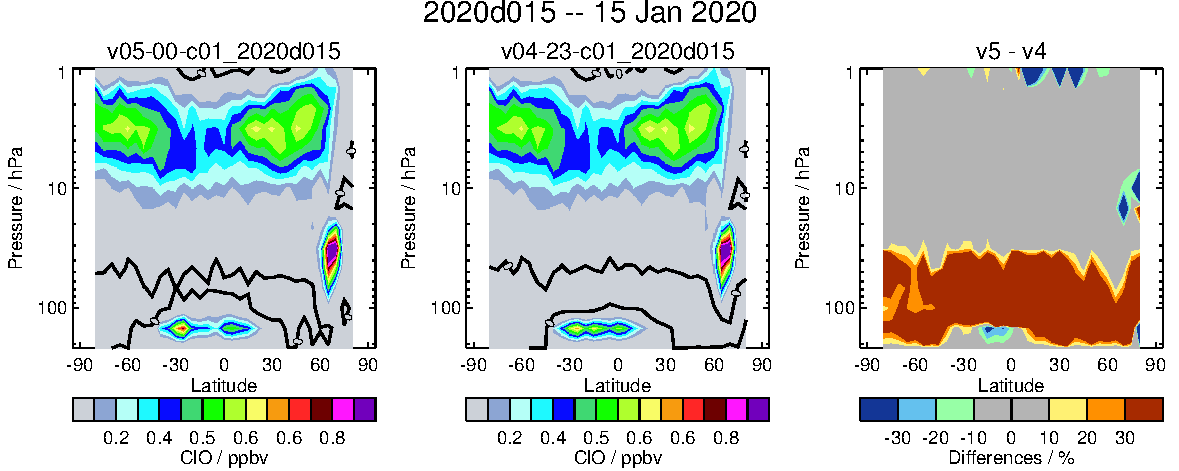
\includegraphics[width=10.0cm]{figures/Zm_ClO_2020d015}
      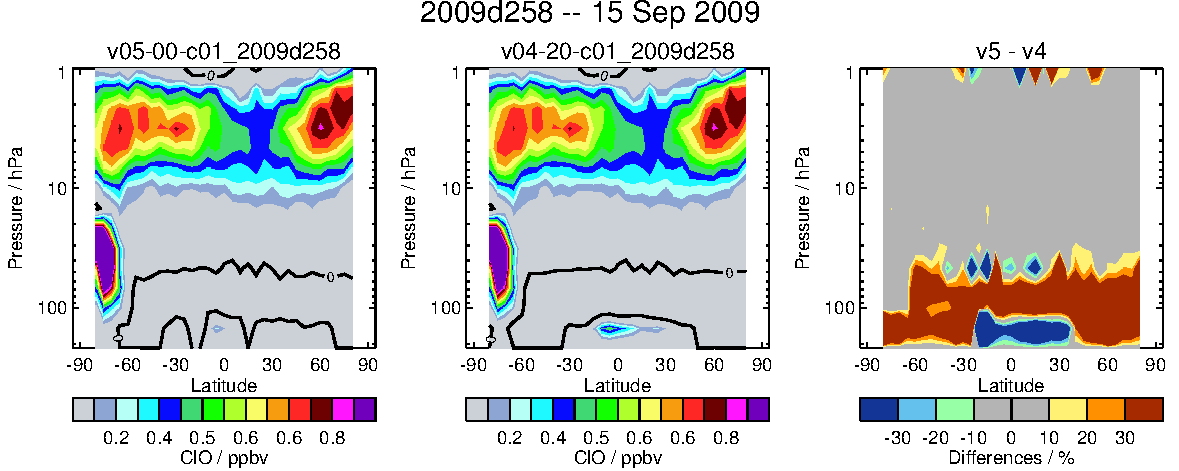
\includegraphics[width=10.0cm]{figures/Zm_ClO_2009d258}
  \end{center}
\caption{Zonal mean pressure-latitude cross sections of MLS daytime
  (ascending) ClO, for (left) \thisv, (middle) \prevv, and (right)
  their differences (\thisv minus \prevv, in percent).  No bias
  corrections have been applied.  Results from a representative day
  with strong ClO enhancement in the winter polar region are shown for
  (top panels) the Northern Hemisphere and (bottom panels) the
  Southern Hemisphere.  The black curves overlaid on the abundance
  panels (left and middle) mark the zero contour.}
\label{fig:zmcontourClO}
\end{figure}

\begin{figure}
  \begin{center}
 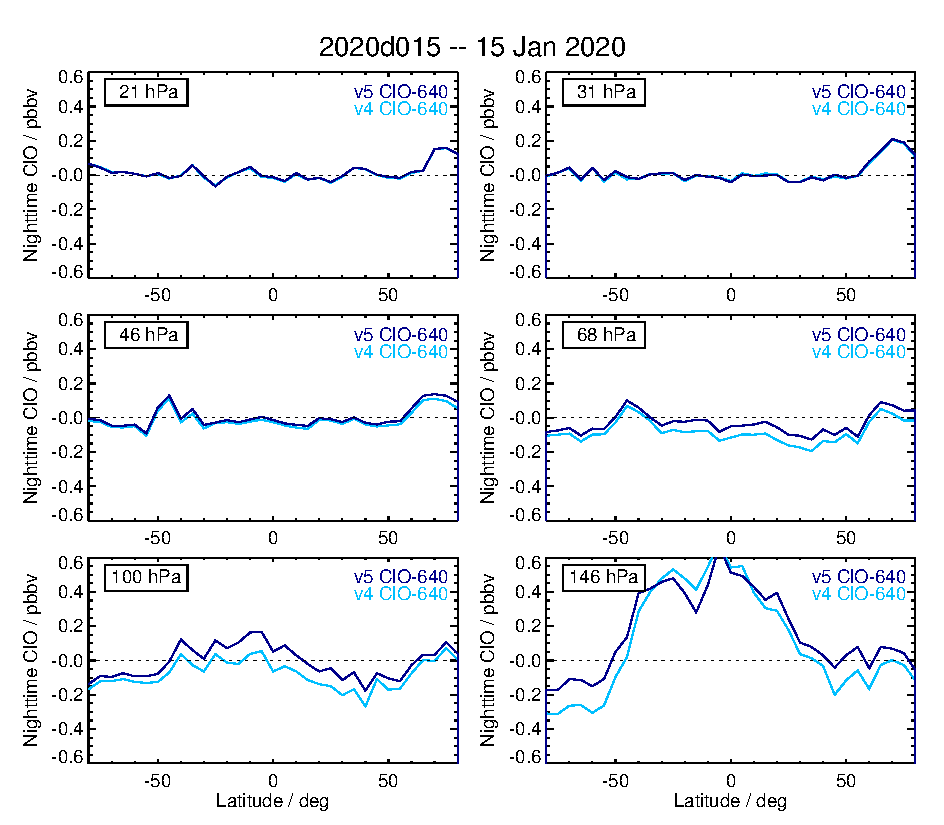
\includegraphics[width=0.48\linewidth]{figures/clov5v4bylat_ClO-640_2020d015}%
 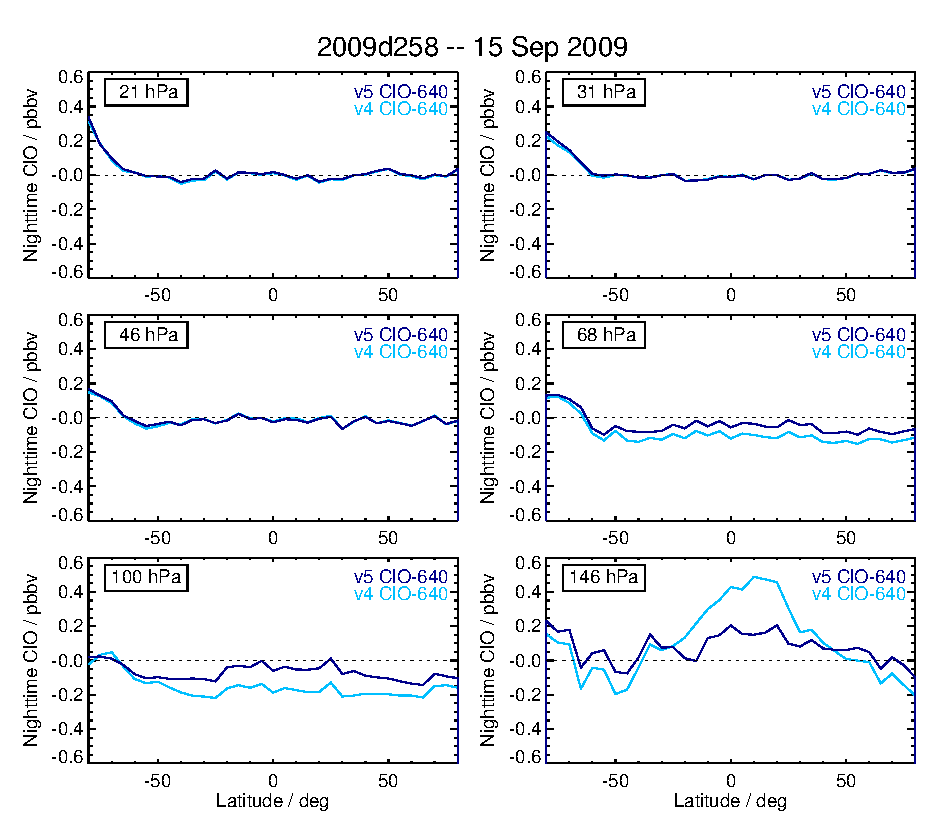
\includegraphics[width=0.48\linewidth]{figures/clov5v4bylat_ClO-640_2009d258}%
   \end{center}
\caption{Nighttime \thisv (dark blue) and \prevv (light blue) MLS ClO
  data as a function of latitude for the six lowest retrieval pressure
  surfaces (21--147\,hPa) for a representative day during winter in
  the Northern (left) and Southern (right) Hemispheres.}
\label{fig:clov3v2bylat}
\end{figure}

\begin{figure}
  \begin{center}   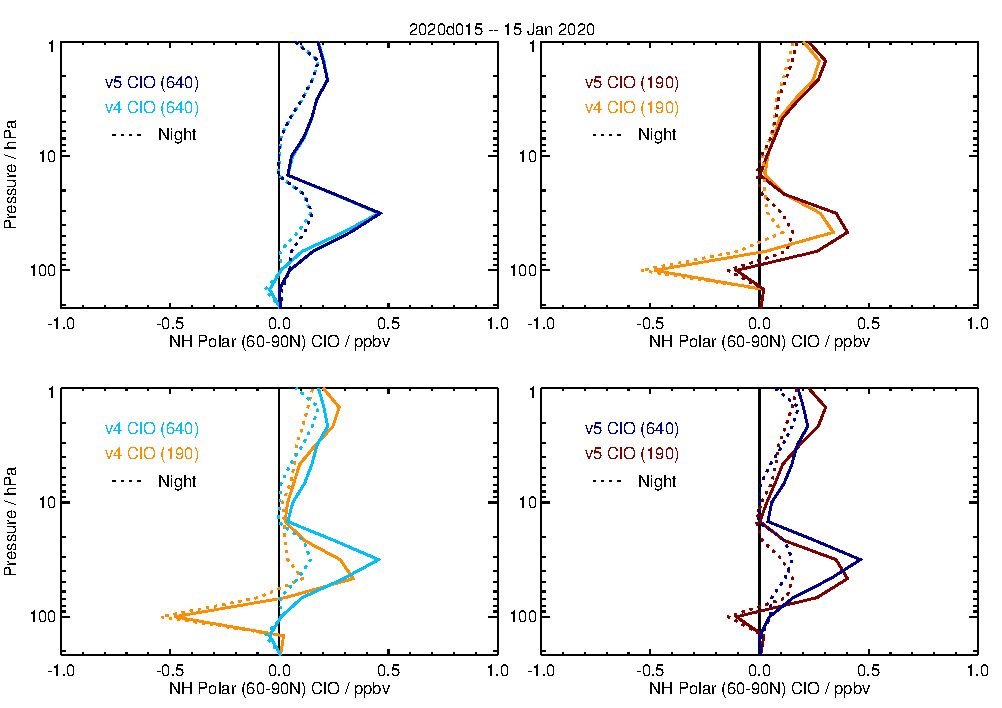
\includegraphics[width=0.48\linewidth]{figures/meanprofcomparison_ClO_2020d015_NHPolar}\hfill    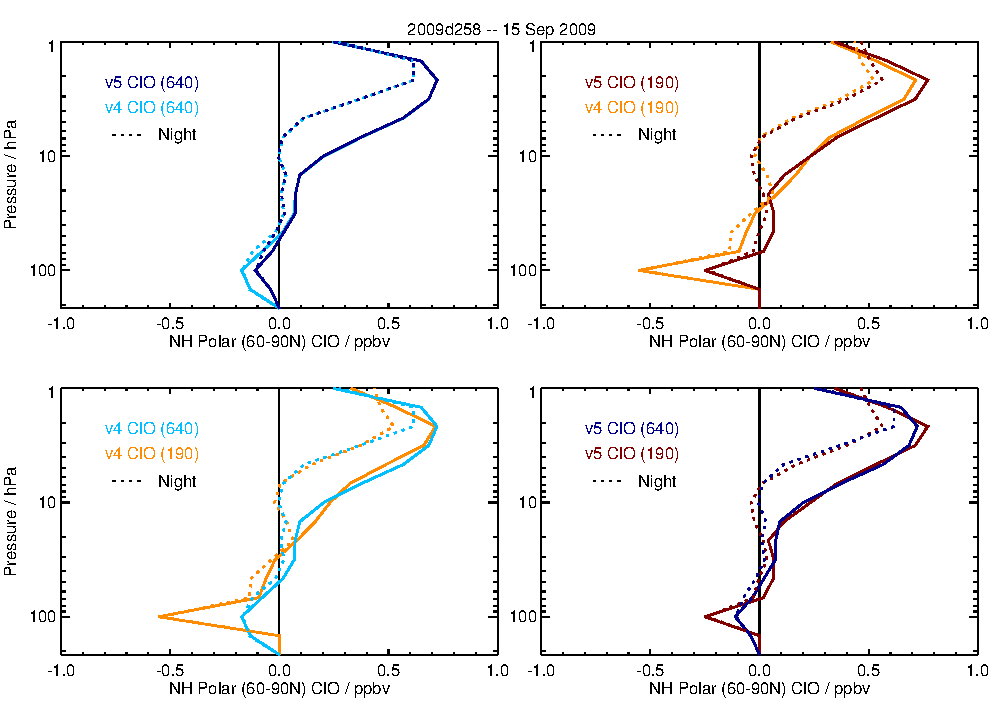
\includegraphics[width=0.48\linewidth]{figures/meanprofcomparison_ClO_2009d258_NHPolar}
  \end{center}
  \begin{center} 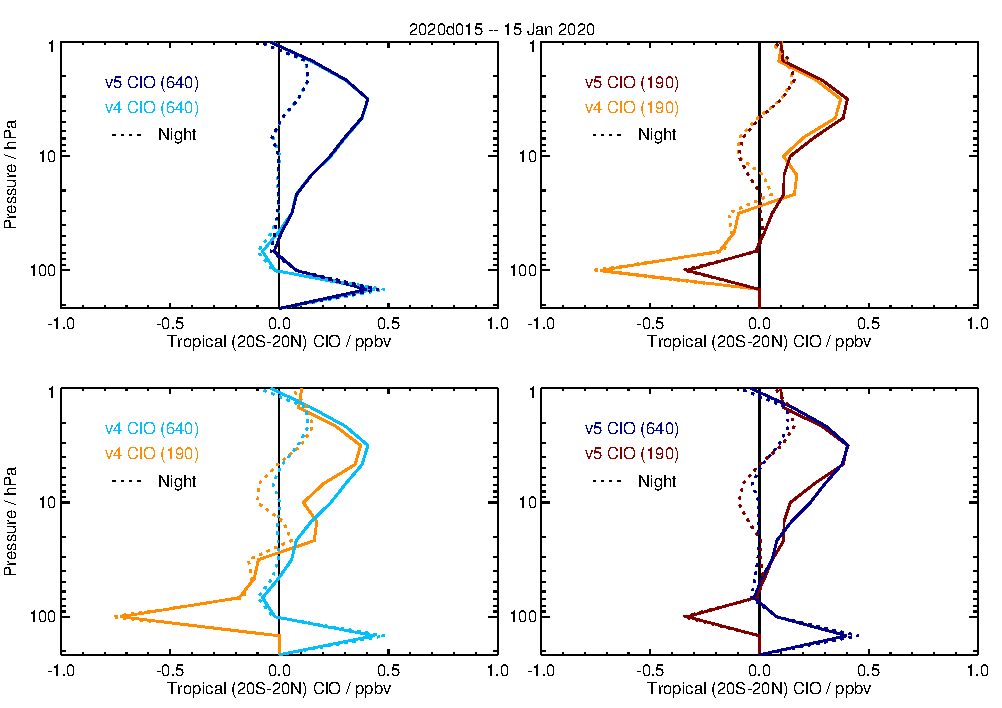
\includegraphics[width=0.48\linewidth]{figures/meanprofcomparison_ClO_2020d015_Tropical}\hfill 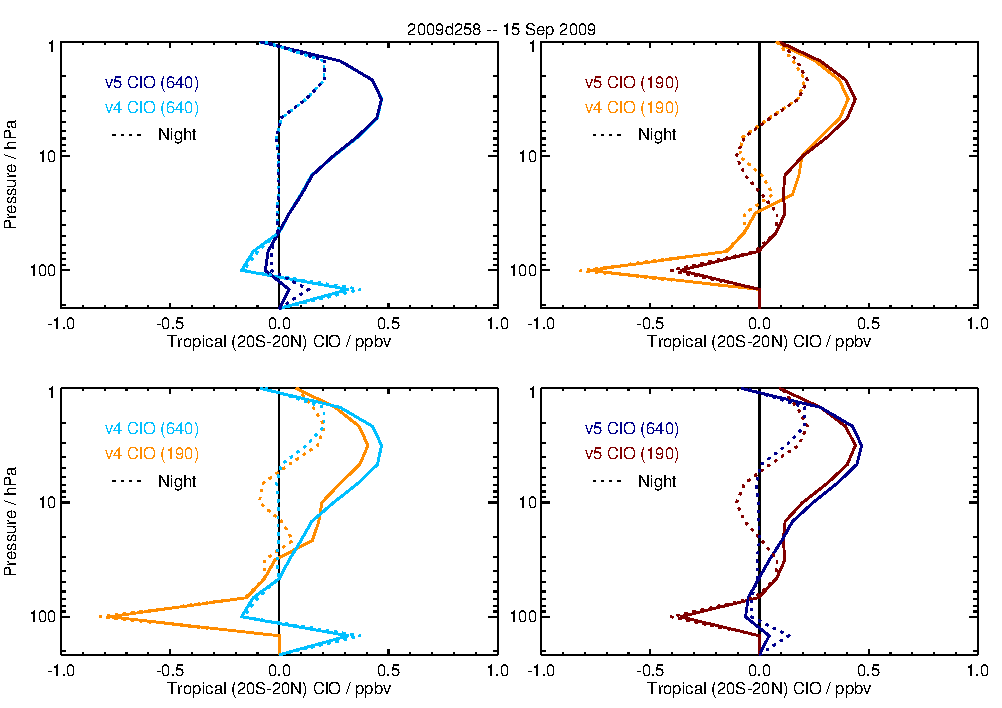
\includegraphics[width=0.48\linewidth]{figures/meanprofcomparison_ClO_2009d258_Tropical}
  \end{center}
  \begin{center}
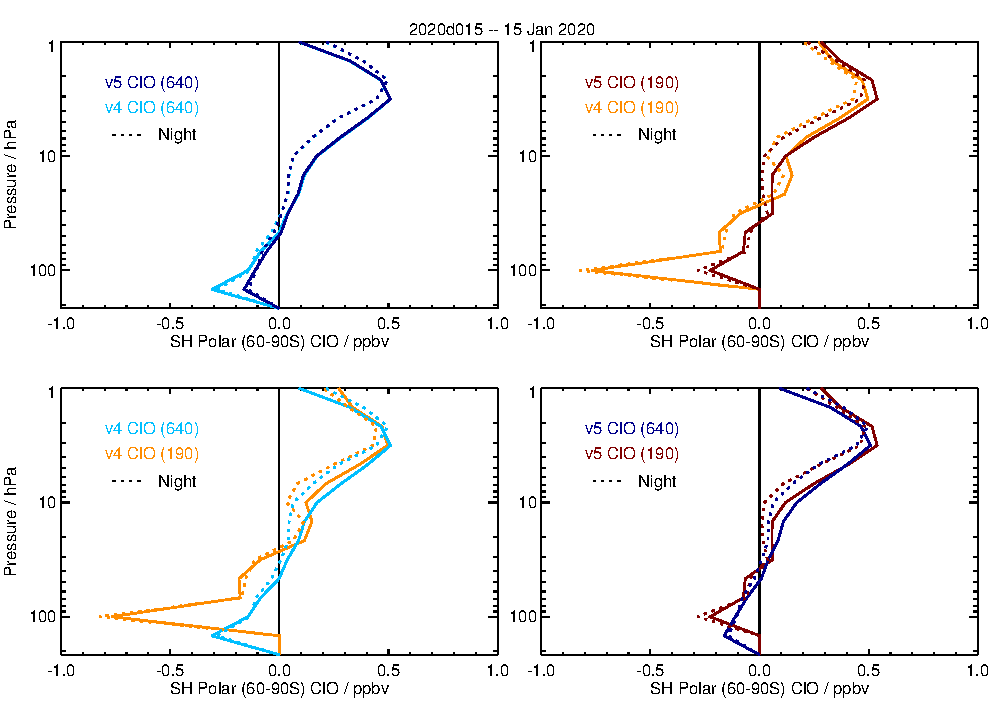
\includegraphics[width=0.48\linewidth]{figures/meanprofcomparison_ClO_2020d015_SHPolar}\hfill 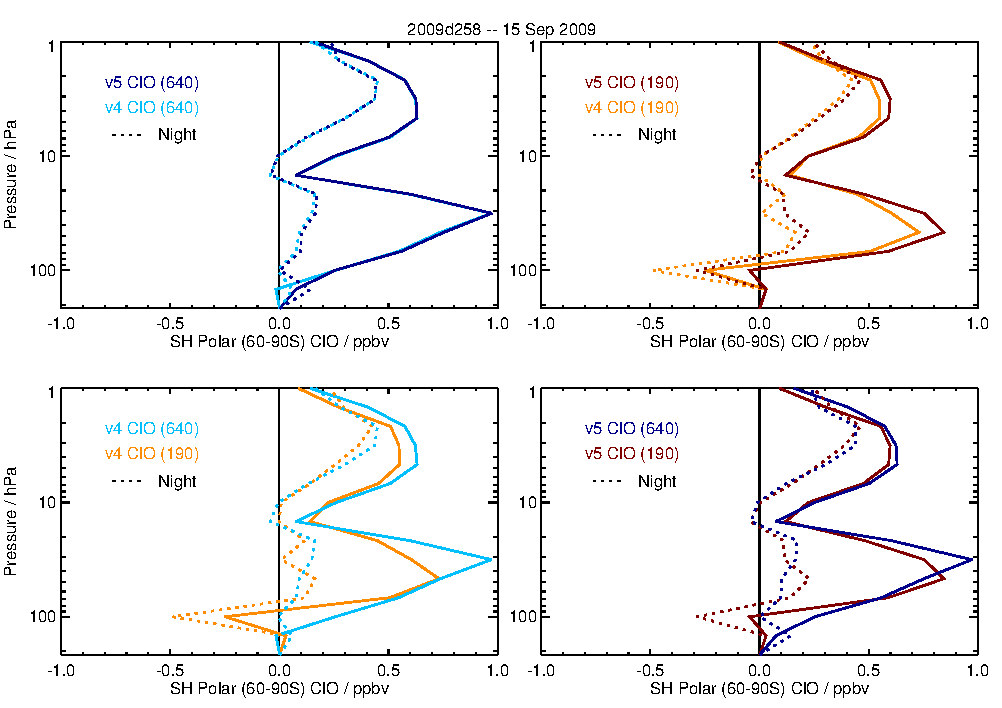
\includegraphics[width=0.48\linewidth]{figures/meanprofcomparison_ClO_2009d258_SHPolar}
  \end{center}
\caption{MLS \thisv (dark colors) and \prevv (light colors) profiles
  of \texttt{ClO-640} (blues) and \texttt{ClO-190} (reds) averaged
  over the Northern Hemisphere polar (top set), tropical (middle set),
  and Southern Hemisphere polar (bottom set) regions for a
  representative day during winter in the Northern (left side) and
  Southern (right side) Hemispheres.  Each set of plots contains four
  panels, comparing \thisv and \prevv \texttt{ClO-640} retrievals,
  \thisv and \prevv \texttt{ClO-190} retrievals, \prevv
  \texttt{ClO-640} and \texttt{ClO-190} retrievals, and \thisv
  \texttt{ClO-640} and \texttt{ClO-190} retrievals.  Solid lines show
  ascending (mainly daytime) and dashed lines show descending (mainly
  nighttime) averages.}
\label{fig:cloMeanProfs}
\end{figure}

Figures~\ref{fig:zmcontourClO}--\ref{fig:cloMeanProfs} show that the
differences between the two versions are larger at the lowest
retrieval pressure levels, where substantial biases present in \prevv
have been ameliorated in \thisv.  To investigate in more detail the
magnitude of and temporal variations in the bias in the \thisv MLS ClO
data and compare them to \prevv, we show in
Figure~\ref{fig:cloBiasByMonth} monthly zonal means of MLS nighttime
ClO measurements for pressure levels 147--46\,hPa.  Each panel
represents a calendar month; nighttime data taken during that month
over the period 2005--2020 have been binned and averaged in
5{\degsym}-wide latitude bands between
$\pm$85{\degsym}. Figure~\ref{fig:cloBiasByPress} is a similar plot
but encompasses all of the MLS nighttime ClO data (i.e., the
climatological annual mean over 2005--2020) for pressure levels
147--10\,hPa.  In both figures, bold colors represent \thisv data,
while corresponding pale colors represent \prevv data.  To guide the
eye, the global-mean annual-mean bias calculated over the
climatological period is indicated for each pressure level (horizontal
solid lines in the respective bold and pale colors).
Figures~\ref{fig:clov3v2bylat}, \ref{fig:cloBiasByMonth}, and
\ref{fig:cloBiasByPress} show that the magnitude, and at 100 and
147\,hPa even the sign, of the bias varies with latitude as well as
pressure.  At 46\,hPa, a negligible negative bias present in \prevv is
further reduced in \thisv.  At 68\,hPa, the small negative bias in
\prevv is considerably lessened but is still evident in \thisv.  At
100\,hPa, the substantial negative bias at higher latitudes (in both
hemispheres) is much smaller, but a slight positive bias is now seen
in the tropics.  At the latter two levels, the magnitude of the
global-mean bias decreased by about half between \prevv and \thisv.
At 147\,hPa, both the large negative bias in the polar regions and the
large positive bias at low latitudes are much smaller, such that the
strong latitude dependence at this level in \prevv has been somewhat
flattened in \thisv.  However, unlike at 68 and 100\,hPa, the global
mean bias has increased slightly at 147\,hPa in \thisv.  In contrast
to the strong altitude and latitude dependence of the ClO bias evident
in these plots, Figure~\ref{fig:cloBiasByMonth} reveals only slight
month-to-month variability in most places.

\begin{figure}
\centering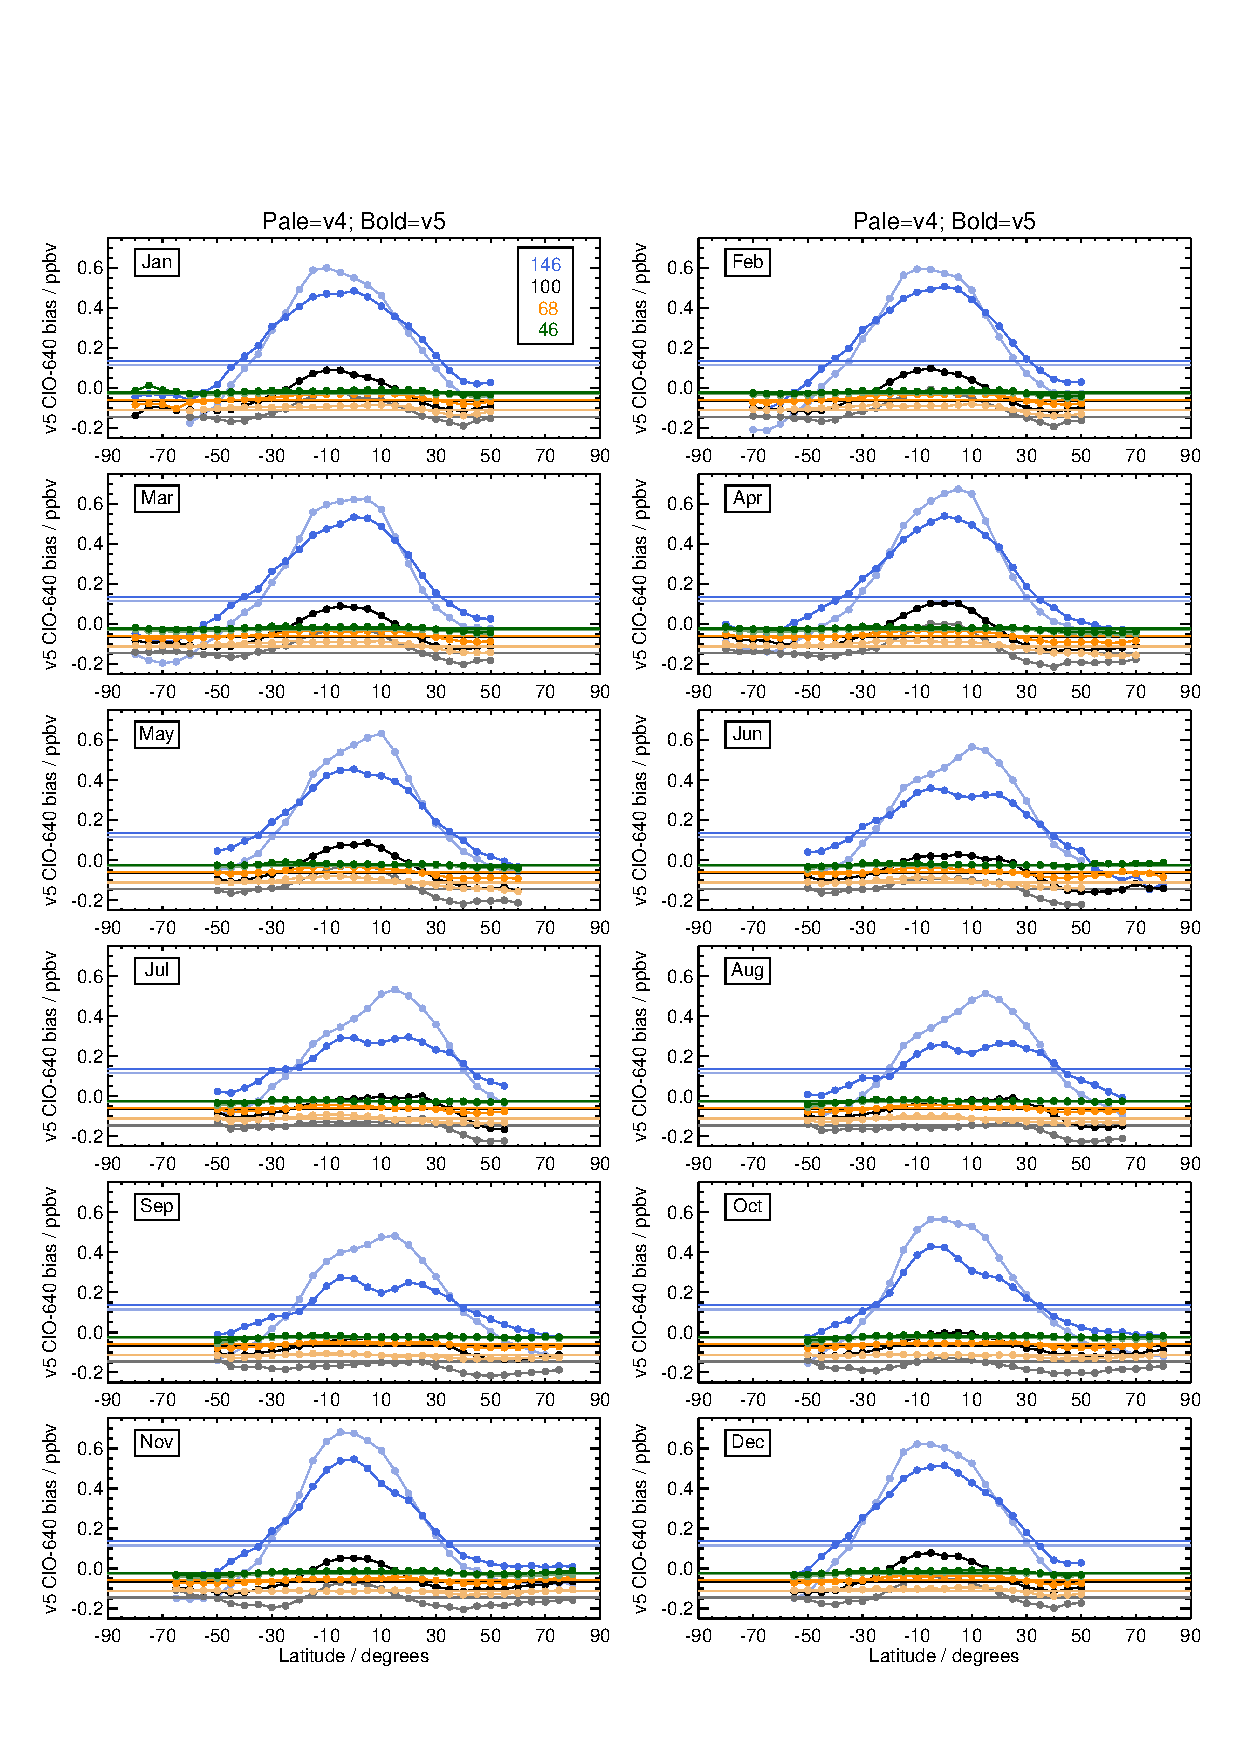
\includegraphics[width=\linewidth,clip=true,trim=0cm 1.5cm 0cm 3.0cm]{figures/plotBiasV5ByMonth-Clim_2020_ClO640}
%\centering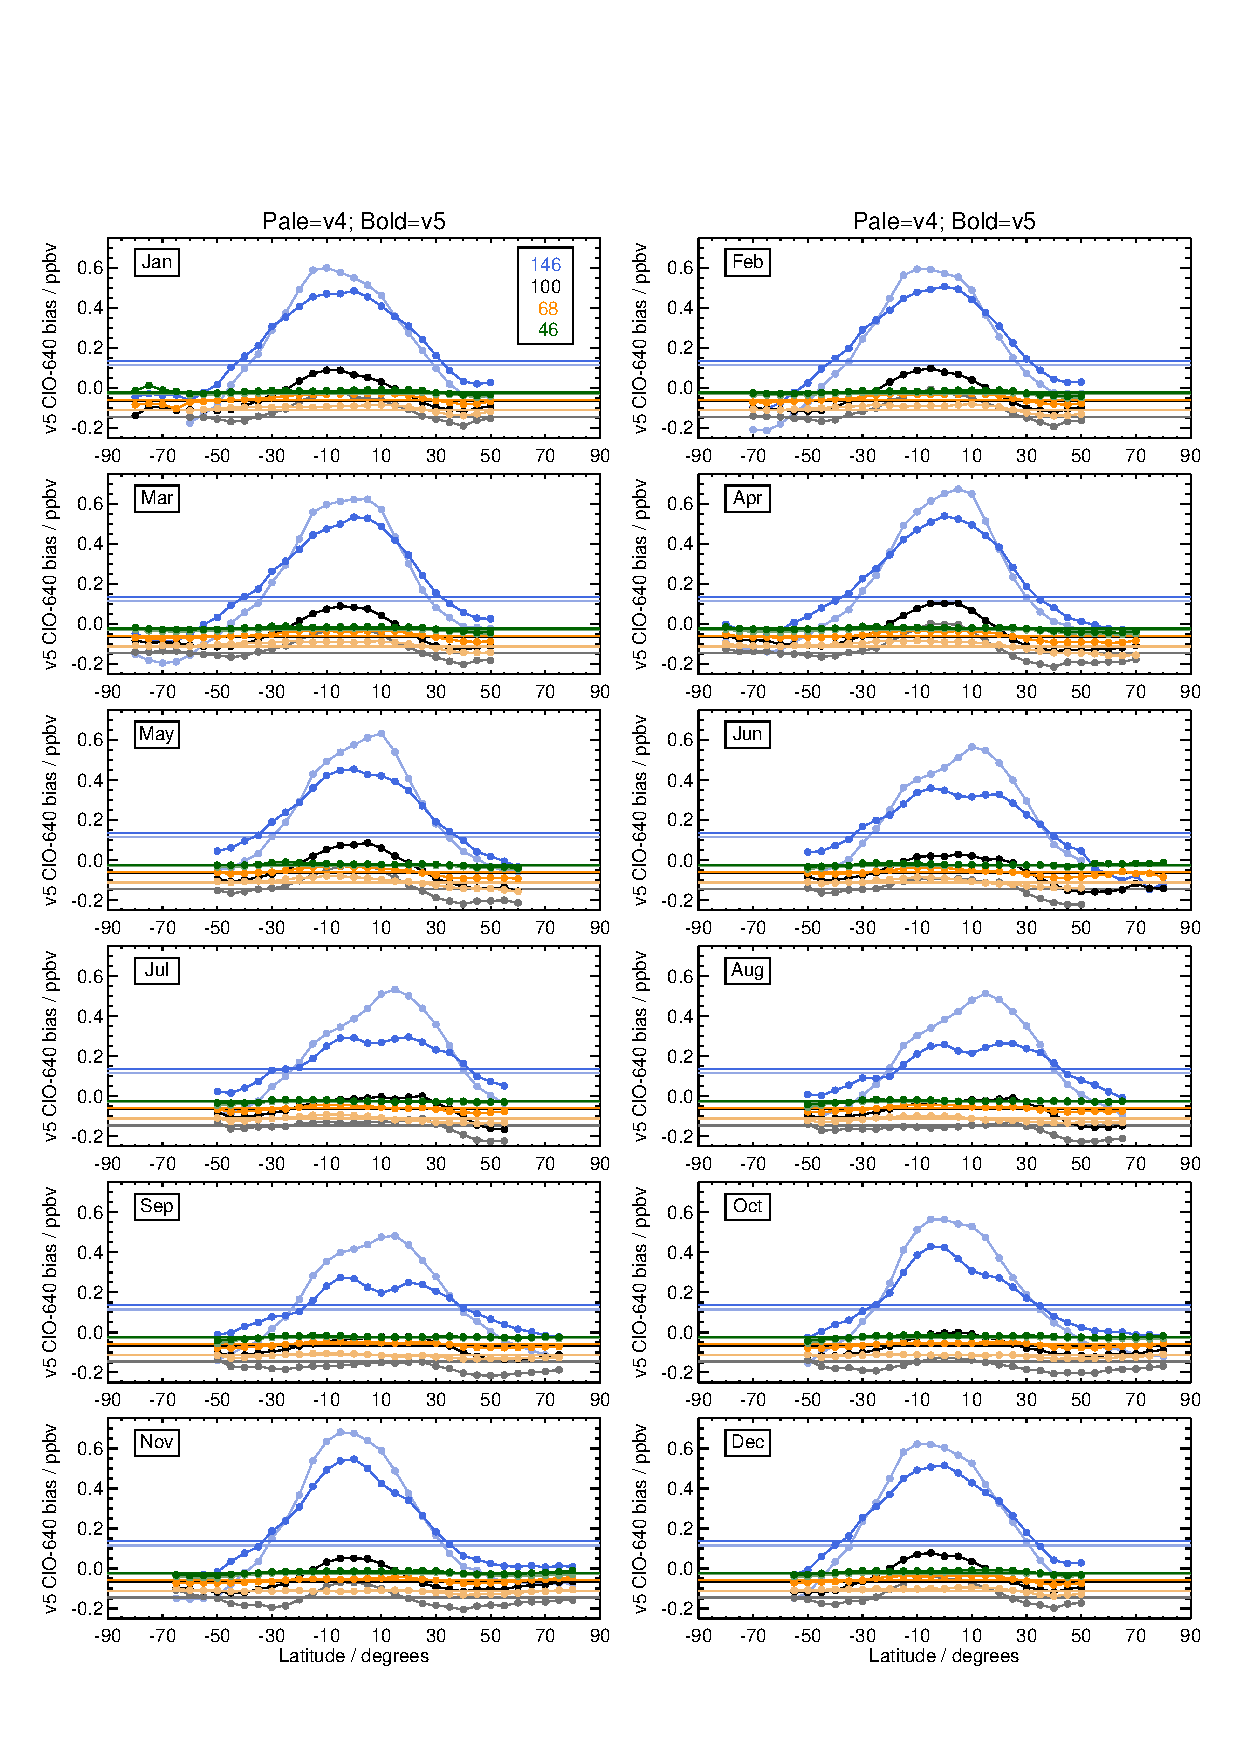
\includegraphics[width=\linewidth]{figures/plotBiasV5ByMonth-Clim_2020_ClO640}
\caption{Estimates of the bias in MLS \thisv ClO data in
  5{\degsym}-wide geographic latitude bands on the 147, 100, 68, and
  46\,hPa MLS retrieval pressure surfaces (see legend).  Each panel
  shows monthly zonal means of \thisv MLS nighttime (solar zenith
  angle $>$ 100{\degsym}) ClO measurements averaged over a
  \mbox{16-yr} period (2005--2020, filled circles). Results for \thisv
  are depicted in bold colors, those for \prevv in corresponding pale
  colors.  The horizontal lines denote the global-mean annual-mean
  bias estimates over the climatological period for both versions at
  each level.  To ensure that ClO was not enhanced, consideration was
  restricted to latitudes equatorward of 50{\degsym}S for the days
  between 1~May and 1~November and to latitudes equatorward of
  50{\degsym}N for the days between 1~December and 1~April.}
\label{fig:cloBiasByMonth}
\end{figure}

In many cases the ClO bias can be essentially eliminated by
subtracting daily gridded or zonal-mean nighttime values from daytime
measurements, and where feasible that is often the preferred
bias-correction approach.  However, it is not practical to do so under
conditions of continuous daylight in the summer or continuous darkness
in the winter at high latitudes.  Moreover, under certain
circumstances during the mid-winter period of peak ClO enhancement
inside the lower stratospheric polar vortices, non-negligible ClO
abundances can be present even in darkness, masking the negative bias.
In this case, computing day$-$night differences considerably reduces
the apparent degree of observed chlorine activation.  Consequently,
for studies of polar chemical processing and chlorine partitioning, it
is instead recommended that an estimate of the bias be subtracted from
the individual measurements at each affected retrieval level.
Attempts to estimate the bias through approaches other than
examination of nighttime ClO measurements (e.g., via correlations with
potentially interfering species, which themselves may vary strongly
with season) have so far met with limited success.  Thus the bias is
estimated from the analysis depicted in
Figure~\ref{fig:cloBiasByPress}.  Although monthly varying bias
estimates might be desirable, as noted above seasonal variations are
small, and it is not possible to directly quantify the bias in the
polar regions during much of the year.  Interannual variations and
longer-term trends (not shown) in the magnitude of the bias are also
small (especially in comparison to the uncertainty in the bias
estimates and the \thisv ClO data themselves; see
Section~\ref{sec:cloacc}).  For these reasons, and to simplify
application of the ClO bias correction for MLS data users, we report
\mbox{16-yr} climatological bias estimates that vary latitudinally and
altitudinally but not temporally; these bias corrections should be
adequate for most studies.  The bias values, reported on a 5{\degsym}
grid, must be interpolated to the MLS Level~2 measurement locations on
each day being considered and subtracted from the ClO mixing ratios
(daytime or nighttime) at those locations.  The bias correction must
be performed \emph{before} interpolation to a different vertical
coordinate (e.g., potential temperature). An ASCII file containing the
estimated ClO bias values has been embedded in the PDF version of this
document; instructions for extracting this file are given in
Appendix~\ref{appsec:ClO}.  The file is also available at
\url{https://mls.jpl.nasa.gov/data/MLS-Aura_ClO-BiasCorrection_v05.txt}.

\begin{figure}
\centering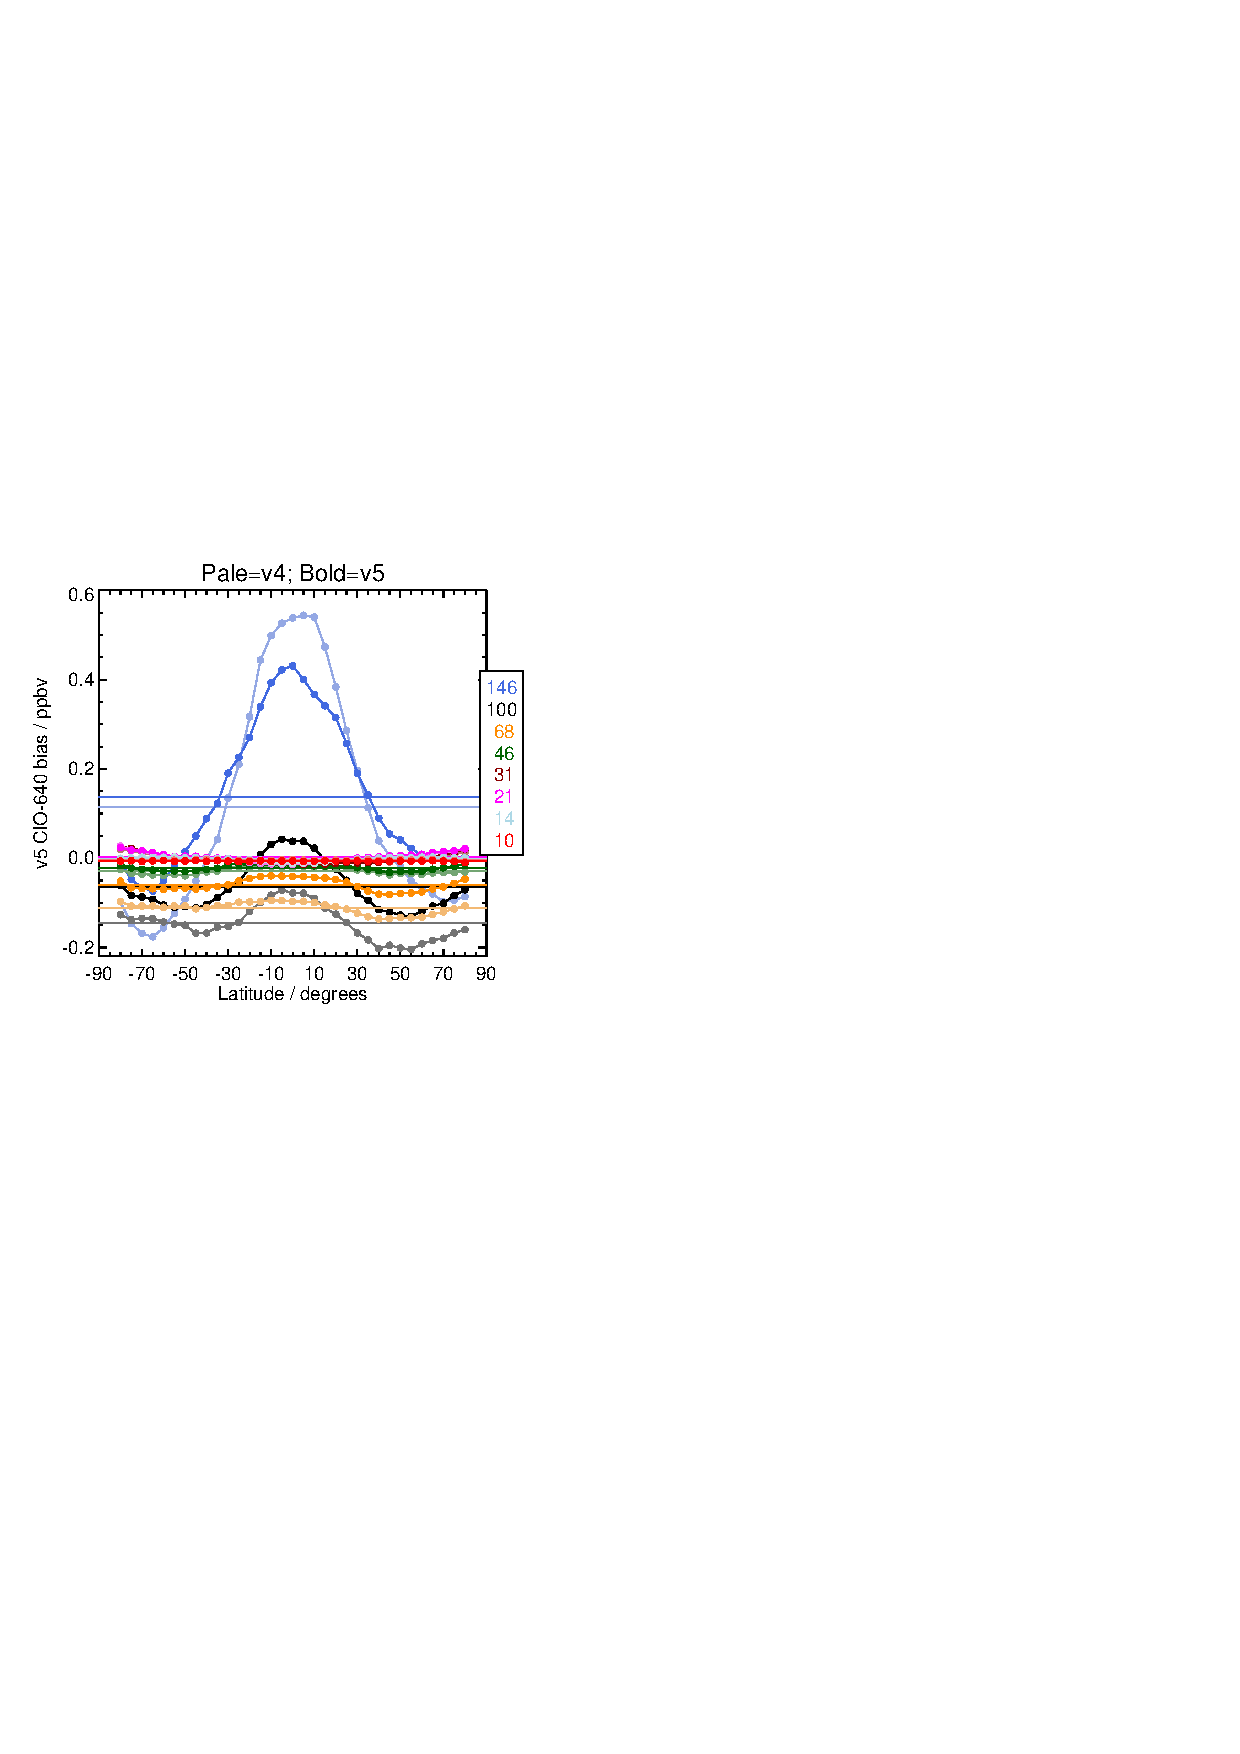
\includegraphics[width=0.6\linewidth,clip=true, trim=0cm 12.6cm 11.0cm 9.0cm]{figures/plotBiasV5-Clim_2020_ClO640}
%\centering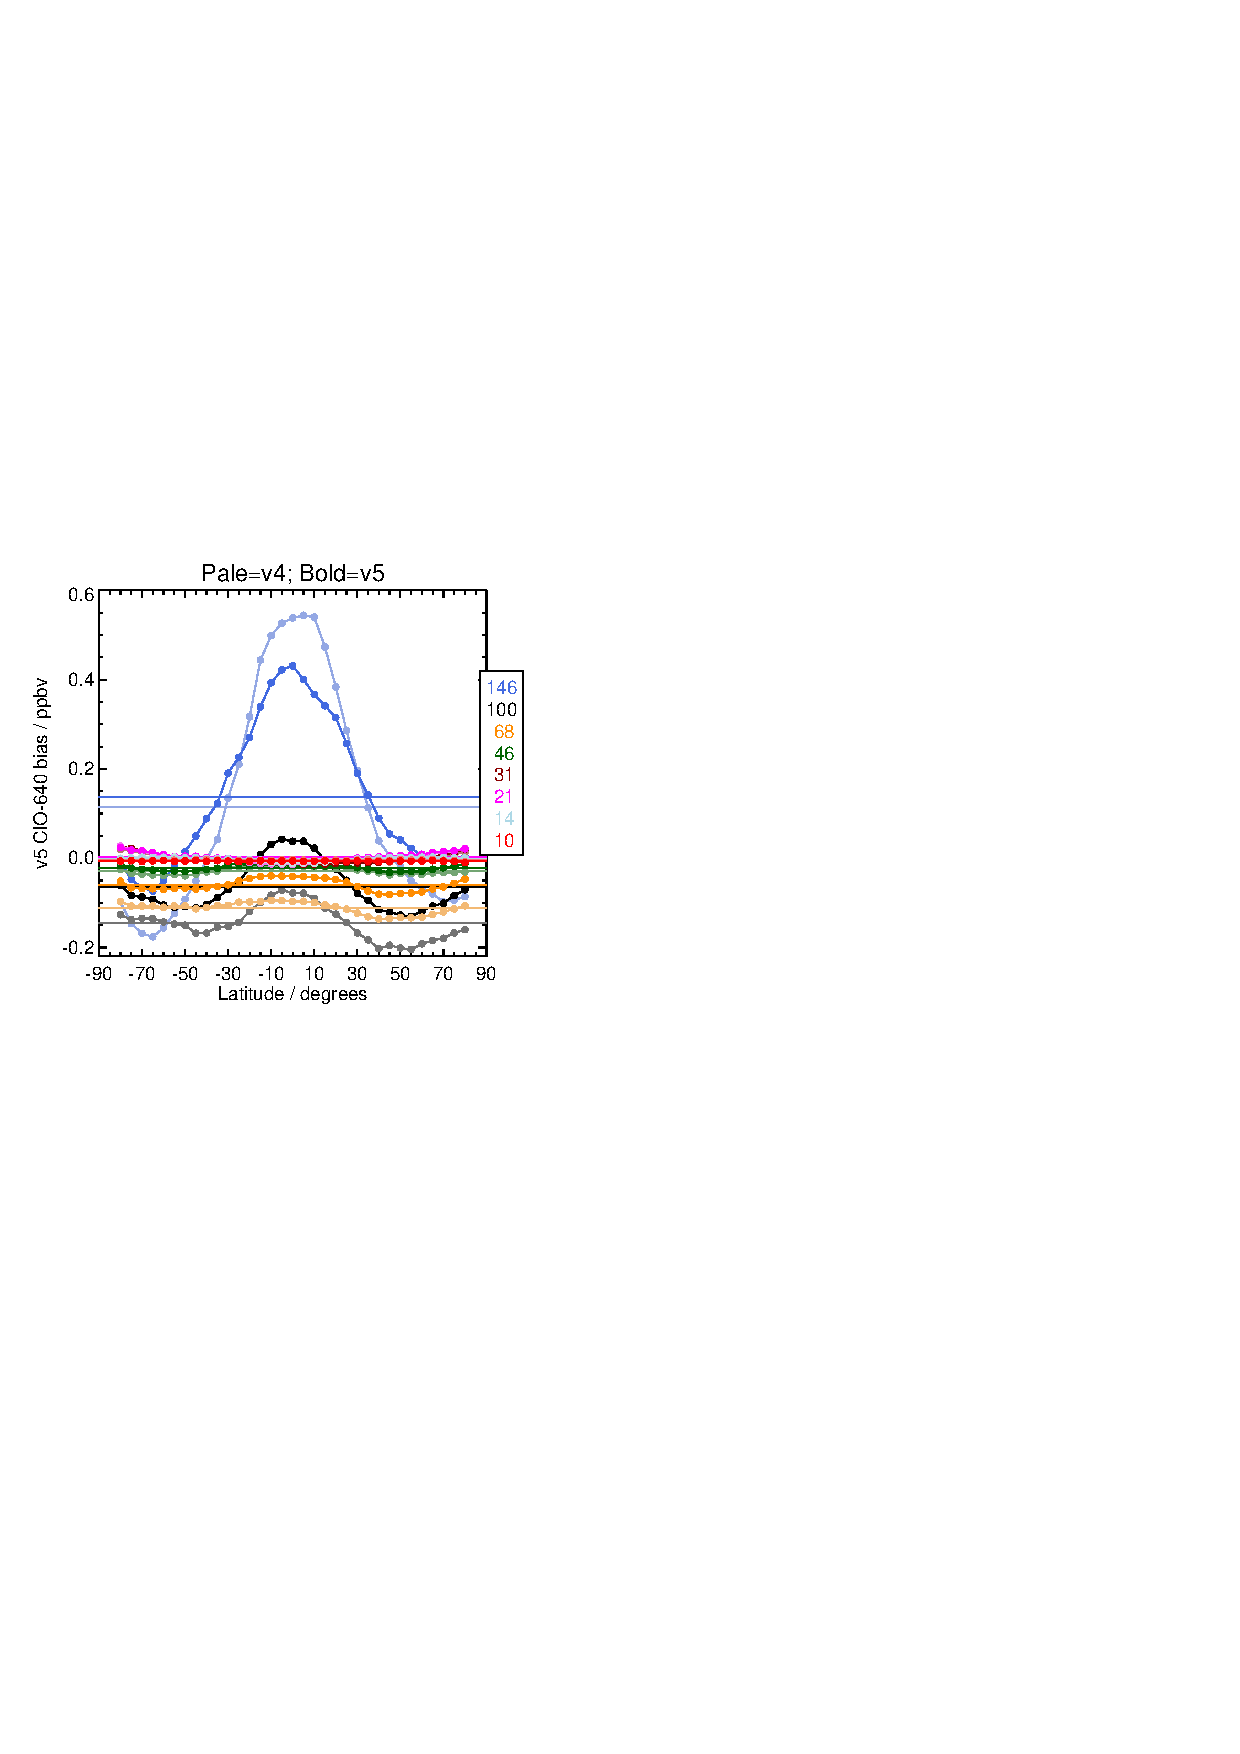
\includegraphics[width=\linewidth]{figures/plotBiasV5-Clim_2020_ClO640}
   \caption{Estimates of the bias in MLS \thisv nighttime (solar
     zenith angle $>$ 100{\degsym}) ClO data in 5{\degsym}-wide
     geographic latitude bands on MLS retrieval pressure surfaces from
     147 to 10\,hPa (see legend) calculated over a \mbox{16-yr} period
     (2005--2020).  Results for \thisv are depicted in bold colors,
     those for \prevv in corresponding pale colors.  The horizontal
     lines denote the global-mean annual-mean bias estimates over the
     climatological period for both versions at each level.  To ensure
     that ClO was not enhanced, consideration was restricted to
     latitudes equatorward of 50{\degsym}S for the days between 1~May
     and 1~November and to latitudes equatorward of 50{\degsym}N for
     the days between 1~December and 1~April.}
\label{fig:cloBiasByPress}
\end{figure}

\subsection{Review of comparisons with other  data sets}

Extensive comparisons of MLS v2.2 ClO data with measurements from a
variety of different platforms (ground-based, balloon-borne, aircraft,
and satellite) were presented by \citet{SanteeEtal:2008:ClO}.  A
subset of those comparisons with v3.3\emph{x}/v3.4\emph{x} ClO data
were reported by \citet{EOSMLSV33V34Quality}.  Comparisons of \thisv
ClO with correlative measurements have not been conducted but are
expected to yield results similar to those for previous versions.

\subsection{Data screening}
\label{sec:ClOScreening}
\begin{description}
\item[Pressure range:] \screeningrule{147--1.0\,hPa}
  \standardrangestatement

  \standardprecisionrule

\item[Status flag:] \screeningrule{Only use profiles for which the
  \texttt{Status} field is zero.}  

  We recommend that all profiles with nonzero values of
  \texttt{Status} be discarded, because of the potential impact of
  cloud artifacts at lower levels.  Note, however, that rejecting in
  their entirety all profiles with nonzero \texttt{Status} may be
  unnecessarily severe at and above (i.e., at pressures equal to or
  smaller than) 46\,hPa, where clouds have negligible impact; thus
  otherwise good-quality profiles with nonzero but even
  \texttt{Status} values may be used without restriction at those
  levels as long as they are removed at larger pressures.  See
  Section~\ref{sec:StatusQuality} for more information on the
  interpretation of the \texttt{Status} field.

\item[Quality:] \qualityrule{1.3} 

  This threshold for \texttt{Quality} (unchanged from \prevv)
  typically excludes less than 0.5\% of ClO profiles on a daily basis;
  note that it potentially discards some ``good'' data points while
  not necessarily identifying all ``bad'' ones.

\item[Convergence:] \convergencerule{1.05} 

  On a typical day this threshold for \texttt{Convergence} (unchanged
  from \prevv) discards very few (0.5\% or less) of the ClO profiles,
  many (but not all) of which are filtered out by the other quality
  control measures.
\end{description}

\subsection{Artifacts}
\begin{itemize}
\item Non-negligible biases are present in both daytime and nighttime
  \thisv ClO mixing ratios at and below (i.e., pressures larger than)
  68\,hPa.  The bias should be corrected by subtracting from the
  individual measurements at each affected retrieval level the
  altitude- and latitude-dependent bias estimates reported in an ASCII
  file that has been embedded in the PDF version of this document;
  instructions for extracting this file are given in
  Appendix~\ref{appsec:ClO}.  This file is also available at
  \url{https://mls.jpl.nasa.gov/data/MLS-Aura_ClO-BiasCorrection_v05.txt}.
\item Care must be taken in interpreting the ClO measurements
  immediately following severe pyrocumulonimbus (pyroCbs) events,
  which can rapidly loft polluted air from the surface and deposit it
  in the lower stratosphere.  Air masses characterized by enhanced
  abundances of biomass burning pollutants may appear to also contain
  elevated levels of ClO, but such apparent enhancements are artifacts
  induced by contamination of the ClO retrieval from methanol
  (CH\cs3OH), a product of wildfires that has a similar spectral
  signature in the MLS band used to measure ClO\@.
\end{itemize}

\subsection{Desired improvements for future data version(s)}
\begin{itemize}
\item Reduce the biases present at the lowest retrieval levels
  (147--68\,hPa).
\end{itemize}

\begin{DIFnomarkup}
\begin{table*}[bp]
\caption{Summary of Aura MLS \thisv ClO Characteristics}\vspace{0.5ex}
\label{tab:ClOSummary}
\begin{minipage}{\linewidth}\small
\renewcommand{\thefootnote}{\thempfootnote}
\centering\begin{tabular}{ccccl}
\toprule
\parbox[m]{18mm}{\bfseries\centering{Pressure\\ / hPa}} &
\parbox[m]{24mm}{\bfseries\centering{Resolution\\ V $\times$ H%
\footnote{Vertical and Horizontal resolution in along-track direction.} \\ / km}} &
\parbox[m]{17mm}{\bfseries\centering{Precision%
\footnote{Precision on individual profiles, determined from observed
 scatter in nighttime (descending) data in a region of minimal atmospheric
 variability.} \\/ ppbv}} &
\parbox[m]{20mm}{\bfseries\centering{Systematic\\ Uncertainty%
    \footnote{Values should be interpreted as \mbox{2-$\sigma$}
      estimates of the probable magnitude and, at the higher
      pressures, are the uncertainties after subtraction of the known
      bias.}\gdef\fnTwoSigma{\value{mpfootnote}}\\ / ppbv}} &
\parbox[m]{40mm}{\bfseries\centering{Known Artifacts\\ or Other Comments}} \\
%
\midrule
%
0.68--0.001 & ---   & ---  & ---  &  Unsuitable for scientific use\\
%
1.0         & 3        $\times$ 500      & $\pm$0.3 & $\pm$0.02 & \\
%
6.8--1.5    & 3.5--4   $\times$ 250--350 & $\pm$0.1 & $\pm$0.02 & \\
%
15--10     & 3.5   $\times$ 250 & $\pm$0.1 & $\pm$0.03 & \\
%
22          & 3        $\times$ 300      & $\pm$0.1 & $\pm$0.05  & \\
%
46--32      & 3        $\times$ 300--400 & $\pm$0.1 & $\pm$0.15  & \\
%
68 & 3 $\times$ 450 & $\pm$0.1 & $\pm$0.2 & Latitude-dependent
bias\footnote{Correct for the bias by subtracting from the individual
  measurements at this level the latitude-dependent bias estimates
  (see Section~\ref{sec:cloBias}).}\gdef\fnDirect{\value{mpfootnote}} \\
%
100         & 3        $\times$ 500      & $\pm$0.1 & $\pm$0.3  & 
Latitude-dependent bias\footnotemark[\fnDirect] \\
%
147         & 4.5      $\times$ 650      & $\pm$0.2 & $\pm$0.6  & 
Latitude-dependent bias\footnotemark[\fnDirect] \\
%
1000--215   & ---   & ---   & --- &  Not retrieved\\
%
\bottomrule
\end{tabular}
\end{minipage}
\end{table*}
\end{DIFnomarkup}

%%% Local Variables: 
%%% mode: latex
%%% TeX-master: "v5-x-report"
%%% End: 


\speciestitle{Carbon monoxide}{CO}{CO}{
  \item[Useful range:] 215--0.001\,hPa
  \item[Contact:] Hugh C. Pumphrey (stratosphere/mesosphere), \email{H.C.Pumphrey@ed.ac.uk} \\ Michael Schwartz (troposphere), \email{Michael.J.Schwartz@jpl.nasa.gov}}

\subsection{Introduction}

Carbon monoxide is retrieved from radiance measurements of two bands in the MLS 240\,GHz radiometer. Full details are given in \citet{PumphreyEtal:2007} and \citet{LiveseyEtal:2008}.

\subsection{Differences between \thisv and \prevv}
The \thisv carbon monoxide (CO) product is extremely similar to the \prevv product, and both are very similar to v04.2x in the upper troposphere and stratosphere, with improvement in some cases relative to v4.2x in the mesosphere and mesopause region, which results from the use of a more computationally expensive, nonlinear forward model for radiances near the 230-GHz line center. Small differences between \thisv and \prevv CO in the upper stratosphere result from changes in the temperature and pointing retrieval, discussed in Section~\ref{sec:StandardTemperature}. 

In the upper mesosphere, \thisv and \prevv CO are less tightly constrained to the \emph{a priori} than is v04.2x CO (\emph{a priori} precision is 1.5$\times$ larger at 0.046\,hPa and 2$\times$ larger at and above 0.01\,hPa). Horizontal smoothing of \thisv has been tightened at and above 0.01\,hPa to maintain retrieval stability, but this change has no appreciable impact on the sharpness of horizontal features seen in preliminary validation. The top of the vertical range of the retrieval remains 0.00046\,hPa and profiles are recommended for scientific use up to 0.001\,hPa.

Figure~\ref{fig:CO_scatv6v5} shows scatter plots of screened \prevv vs.\ \thisv CO from 215\,hPa to 0.01\,hPa during 2009, showing that the two versions are almost identical. 
High outlier values of CO along the 1:1 lines of panels for 216--46.4\,hPa in Figure~\ref{fig:CO_scatv6v5} are measurements within the plume from the ``Black Saturday'' Australian wildfires and confirm the consistency of the \thisv and \prevv retrievals in the upper troposphere and lower stratosphere, even when unusally high values are retrieved .

The calculation of cloud flags bits in the product status has changed significantly in \thisv, as is discussed in Section~\mycomment{Point to appropriate section}.  \Thisv CO has approximately twice as many profiles marked as possibly influenced by low cloud than \prevv, and no profiles flagged as influenced by only high clouds.  Neither of these flags is used in the recommended screening.
\subsection{Resolution}
\onestandardavk{CO}{CO}%

Figure~\ref{fig:AvkCO} shows the horizontal and vertical averaging kernels for \thisv MLS CO\@. Estimated vertical and horizontal resolutions are essentially identical to those of \prevv and v04.2x. The vertical resolution is in the range 3.5--5\,km from the upper troposphere to the lower mesosphere, degrading to 6--7\,km in the upper mesosphere. Down to the 215\,hPa level, the vertical averaging kernels are sharply peaked at the level being retrieved, but while the \mbox{316-hPa} measurement contains contribution from 316\,hPa, it has a larger contribution from 215\,hPa and a negative contribution around 100\,hPa of similar magnitude to that at 316\,hPa. The retrieved value at 316\,hPa is thus more an extrapolation of the profile higher in the UTLS than it is an independent measurement at 316\,hPa, and it is not recommended for scientific use. The horizontal resolution is about 200\,km in the mesosphere, degrading slowly to 300\,km with decreasing height in the stratosphere and more rapidly to about 460\,km at 100\,hPa and 690\,km at 215\,hPa.

\begin{figure}
  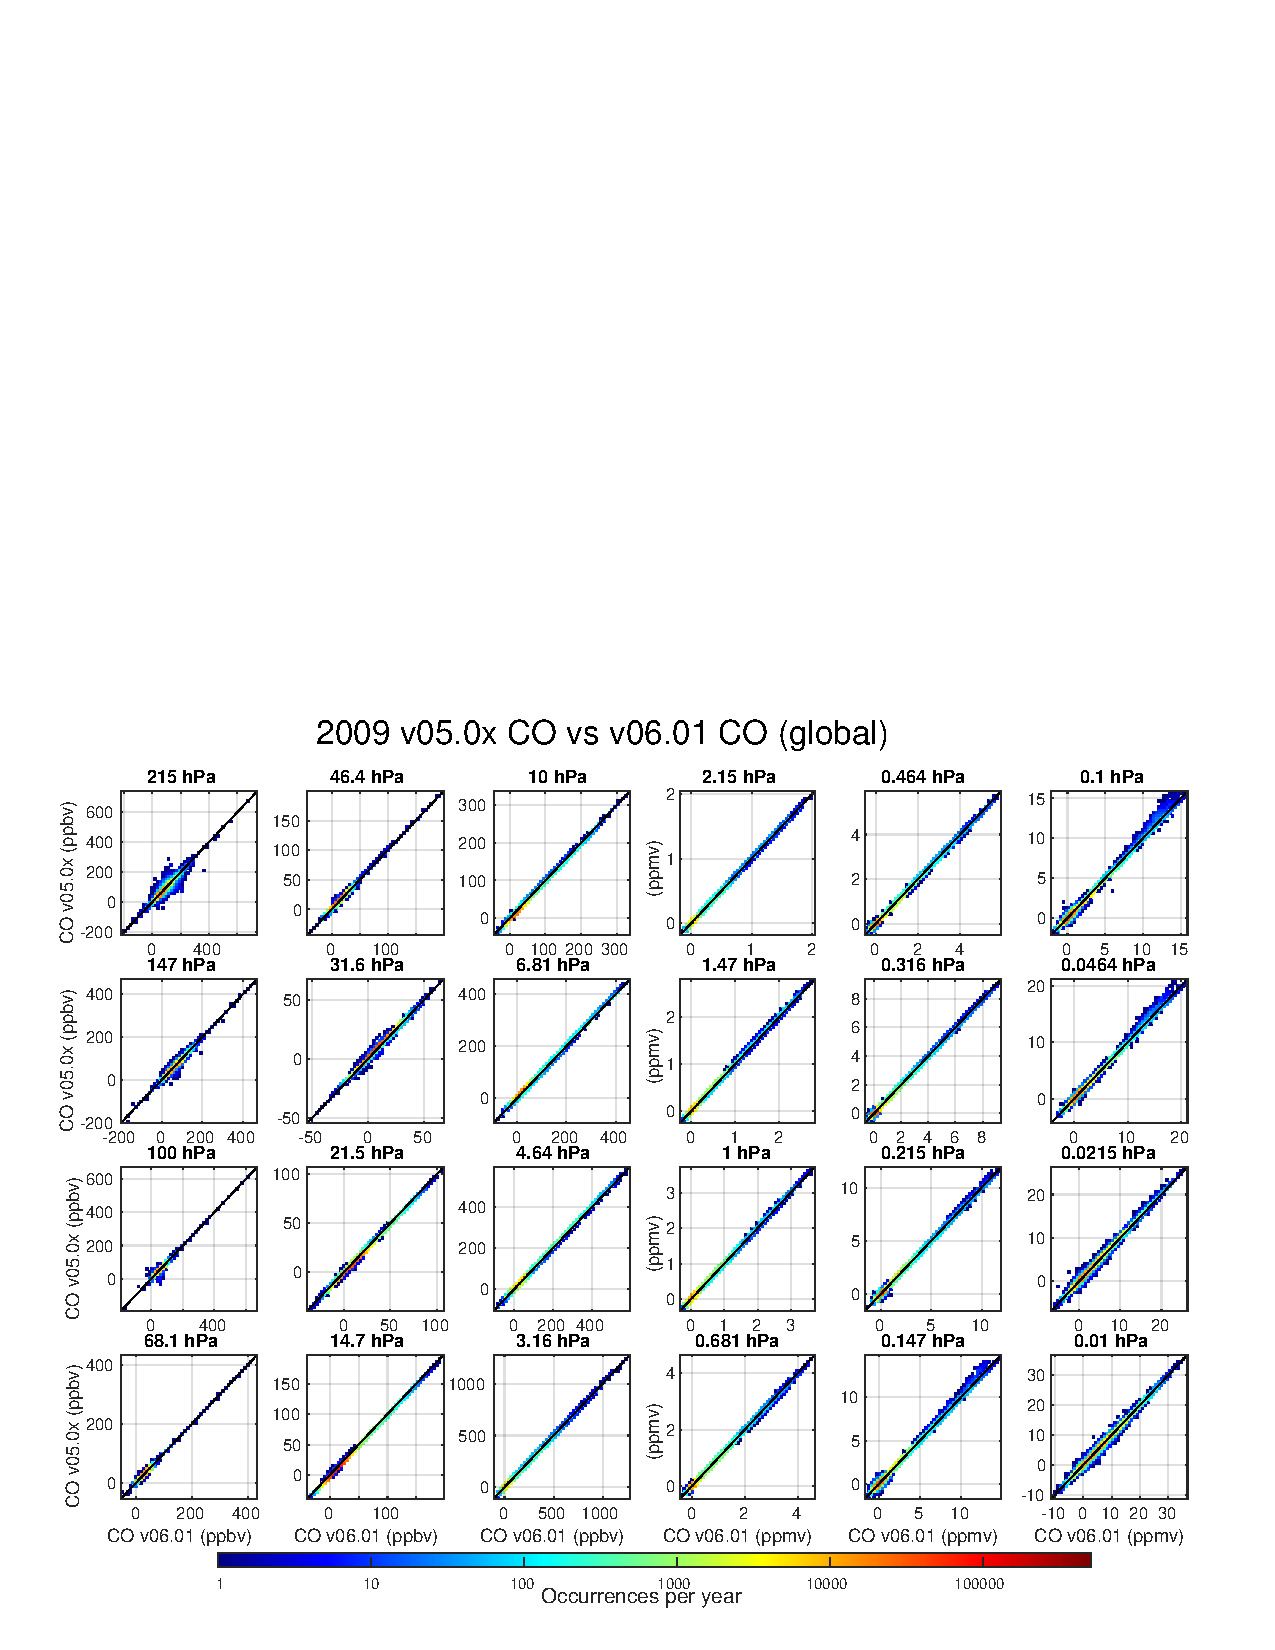
\includegraphics[width=\textwidth, trim=1.4cm 1cm 1.8cm 12.5cm]{figures/CO_scatv6v5}
  \caption{Joint histograms of \prevv CO and \thisv CO for 2009 data show the general consistency of the two versions.  The color scale is logarithmic, with red points along the 1:1 line corresponding to pairs of values that are identical in the two versions. }
  \label{fig:CO_scatv6v5}
\end{figure}

\subsection{Precision}

The MLS data are supplied with an estimated precision (the field \texttt{L2gpPrecision}) which is the \emph{a posteriori} precision as returned by the optimal estimation. The precision of the \thisv CO is nearly identical to that of \prevv, and very similar to that of v04.2x. Reported precision is greater than the scatter observed in the data in regions of low natural variability. This can be seen in the middle (low-latitude) panels of the second row of Figure~\ref{fig:COplot1bylat_log}, where the purple and yellow solid lines (scatter about the zonal means) have smaller values than the purple and yellow dashed lines (precisions). Where the estimated precision is greater than 50\% of the \emph{a priori} precision the data will be influenced by the \emph{a priori} to an undesirably large extent. In such cases, \texttt{L2gpPrecision} is set to be negative (or zero in some cases) to indicate that the data should not be used. The \thisv\mycomment{Verify this?} \emph{a priori} precision has been relaxed above 0.1\,hPa (blue dashed line departing from red dashed line in center panels of Figure~\ref{fig:COplot1bylat_log}), and the level at which the retrieved precision is more than half of this \emph{a priori} precision typically moves up from 0.0046\,hPa to 0.00046\,hPa.

\begin{figure}
  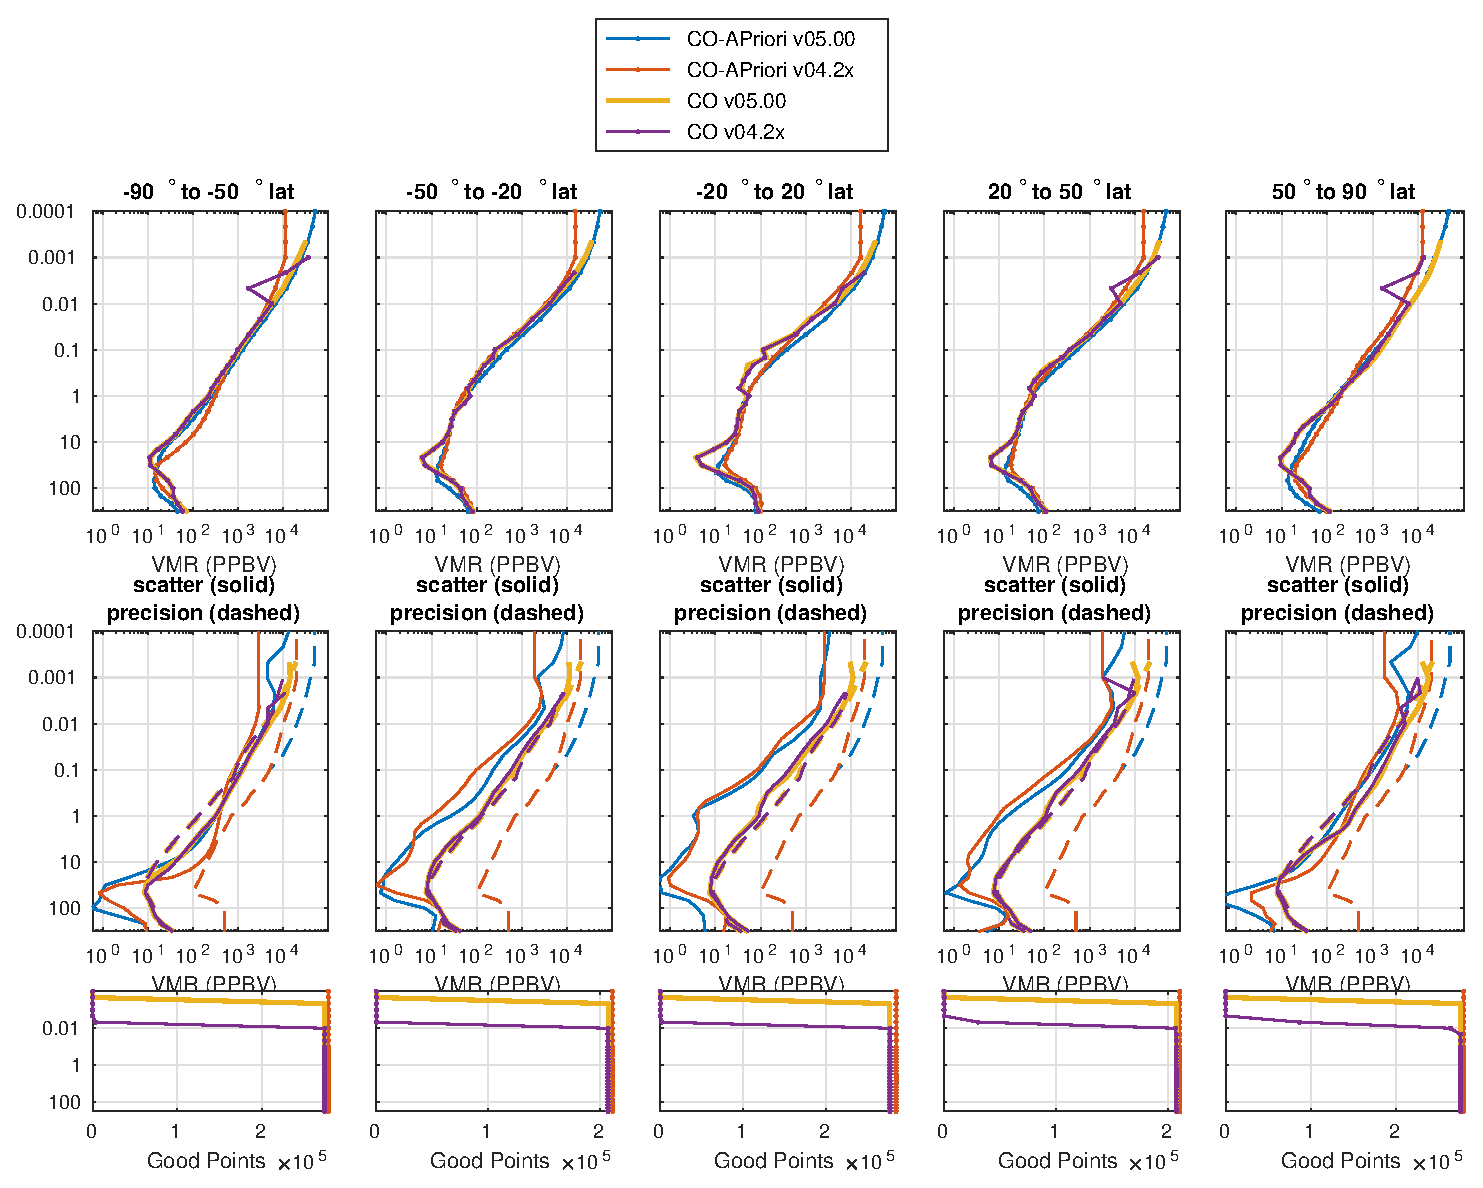
\includegraphics[width=\textwidth]{figures/COplot1bylat_log}
  \caption{\mycomment{This figure is still old, right?} The top row shows 2009 zonal means of \thisv\CheckThis and \prevv\CheckThis mixing ratios and their \emph{a priori} values.  The \prevv\CheckThis retrieved mixing ratio line (purple) lies on top of the \thisv\CheckThis mixing ratio line (yellow) for all but the highest altitude pressure surfaces, despite significant differences in their \emph{a priori} profiles. The middle row shows the zonal scatter about these zonal means (solid lines) and corresponding estimated precisions (dashed lines).  The bottom row shows the number of good profiles, limited at the highest retrieval levels where retrieved precision exceeds half of the \emph{a priori} precision.}
  \label{fig:COplot1bylat_log}
\end{figure}

Note that the random errors (precisions) are larger than 100\% of the mixing ratio for much of the vertical range, meaning that significant averaging (e.g., daily zonal mean or weekly map) is typially needed to make use of the data.

\subsection{Accuracy}
The estimated accuracy is summarized in Table~\ref{tab:COSummary}. In the middle atmosphere the accuracies are estimated by comparisons with the ACE-FTS instrument; see \citet{PumphreyEtal:2007} for further details. The MLS v2.2 CO data at 215\,hPa showed high (factor of \mytexttilde2) biases compared to other observations. The morphology, however, was generally realistic \citep{LiveseyEtal:2008}. In \thisv (as in \prevv) this bias has been essentially eliminated through a change in the approach to modeling the background radiance upon which the CO spectral line sits, and a small reduction in the number of MLS spectral channels considered in the retrieval. Tropospheric (215--100\,hPa) accuracies in Table~\ref{tab:COSummary} are 2-$\sigma$ estimates obtained by propagating parameter uncertainties through a model of the measurement system, and are unchanged from those calculated for \prevv.

\subsection{Data screening}
\label{sec:COScreening}
\begin{description}
  \item[Pressure range:] \screeningrule{215--0.001\,hPa.} \standardrangestatement\ Data at 0.00046\,hPa represents a total column at and above that pressure level. Scientific use of these 0.00046\,hPa data may be possible, but consultation with the MLS team is advised. \standardprecisionrule \evenstatusrule

  \item[Clouds:] Clouds have no impact for pressures of 31\,hPa or less. \thisv, \prevv and v04.2x CO are much less susceptible to cloud-induced artifacts than was v03.x, so screening of the CO product is considerably simplified compared to that recommended for v03.x, needing only application of the standard \texttt{Quality} and \texttt{Convergence} rules as described below. The low-cloud status bit, which was set for 0.2\% of profiles in \prevv, is set for 0.6\% of profiles in \thisv, but preliminary validation does not find this flag to be useful for data screening.

  \item[Quality:] \screeningrule{Only use profiles with \texttt{Quality} greater than 1.5.} Profiles with \texttt{Quality} less than or equal to 1.5 comprise 0.7\% of all data, and \mytexttilde2\% of profiles in the tropics. At 215 hPa in the tropics, the rejected profiles have mixing ratios that are, on average, 7\% higher than other tropical values and the occurrence rates of high outliers with mixing ratios greater than 150\,ppbv is about twice that of the rest of the tropical ensemble. At 100\,hPa there is no significant difference in the means of tropical profiles with Quality less than or greater than 1.5.

  \item[Convergence:] \convergencerule{1.03} This \texttt{Convergence} criterion rejects fewer than 0.1\% of profiles. Almost all of the retrievals in the phase that produces \thisv CO converge to their target, so \texttt{Convergence} is of limited use in screening.
\end{description}

\subsection{Artifacts}
\begin{itemize}
  \item Positive systematic error of 20--50\% throughout the mesosphere, as was the case for \prevv.
  \item Negative systematic error of 50--70\% near 30\,hPa, as was the case for \prevv.
  \item Retrieved profiles are rather jagged, especially between 1\,hPa (48\,km) and 0.1\,hPa (64\,km). The greater smoothing applied in \thisv, \prevv, v04.2x and v03.3 compared to v2.2 reduced this problem considerably but has not eliminated it entirely.
  \item The tendency for negative values to occur at the level below a large positive value that was present in v04.2x is somewhat reduced in \thisv and \prevv.
  \item Upper-tropospheric \thisv CO retrieved values still show some anomalous sensitivity to thick clouds associated with deep convection. The screening procedure based upon \texttt{Quality} and \texttt{Convergence} that is described above is generally effective in removing these artifacts.
  \item Negative outliers in UT CO have been observed in volcanic plumes, such as that from the eruption of Sarychev in June of 2009. These are likely the result of interference from spectral lines of a gas-phase plume component, and are a subject for further analysis and validation.
\end{itemize}

\subsection{Review of comparisons with other datasets}

In the upper troposphere, comparisons with various in situ CO observations (NASA DC-8, WB-57 and the MOZAIC dataset) indicate that the \emph{earlier} MLS v2.2 215\,hPa CO product was biased high by a factor of \mytexttilde2. As in v04.2x and \prevv, this bias is largely eliminated in \thisv.

In the mesosphere, comparisons of the earlier v2.2 MLS CO with ODIN-SMR and ACE-FTS suggest a positive bias: 30\%--50\% against ACE-FTS, 50\%--100\% against SMR. Near 31\,hPa, the MLS values are lower than SMR and ACE-FTS by at least 70\%. The MLS values have not changed much between v2.2 and \thisv in the middle atmosphere, so these comparisons may mostly be considered valid for \thisv. What change there was between v2.2 and later versions consists of a slight lowering of the MLS values, bringing them slightly towards the ACE-FTS data; 20\% is now a better estimate of the MLS-ACE bias in much of the middle atmosphere (compared to 30\% with v2.2).
% Mean difference between \prevv\CheckThis and \thisv\CheckThis in the lower mesosphere
% are still generally small.
Further validation of the \thisv retrieval above 0.01\,hPa is needed.

\begin{table}
  \caption{Data quality summary for MLS \thisv CO.}
  \vspace{\tablecaptionsep}
  \label{tab:COSummary}
  \begin{minipage}{\linewidth}
    \centering\begin{tabular}{ccccl}
\toprule
\textbf{Pressure} &
\textbf{Resolution / km} & 
\textbf{Precision} / &
\textbf{Accuracy} &  
\textbf{Comment} \\
\textbf{/ hPa} &
\textbf{Vert $\times$ Horiz.} &
\textbf{ppbv} \\
\midrule
$<0.001$  &    ---        &   ---   &    ---      & Not retrieved\\
0.00046  & ---       &   ---   &    ---    & Unsuitable
for scientific use \\
0.001  &   7.2   $\times$ 200 &  12000  & validation needed & possibly use, with caution\\
0.0022 &   5.9   $\times$ 200 &  8700  & validation needed  & possibly use, with caution \\
0.0046 &   5.8   $\times$ 200 &  6000  &   $+$20\% to $+$50\%     &  \\
0.01   &   5.9   $\times$ 200 &  3400   &   $+$20\% to $+$50\%  &  \\
0.046  &   5.9   $\times$ 200 &  1000   &    $+$20\% to $+$50\%    &  \\
0.14   &   3.8   $\times$ 200 &  640    &    $+$20\% to $+$50\%    &  \\
1      &   4.1   $\times$ 250 &  120    &    $+$20\% to $+$50\%  &  \\
10     &   5.0   $\times$ 440 &  16     &    $\pm 10$\%    &  \\
31     &   4.9   $\times$ 400 &   9     &    $-$70\% to $-$50\%    &  \\
100    &   4.9   $\times$ 450 &  14     & $\pm$19\,ppbv and $\pm$30\%
\footnote{Estimated 215--100 hPa systematic uncertainty is the RSS of the additive and multiplicative terms.} & \\
147    &   5.1   $\times$ 570 &  16     & $\pm$26\,ppbv and $\pm$30\% & \\
215    &   5.4   $\times$ 690 &  19     & $\pm$38\,ppbv and $\pm$30\% \\
316 & --- & --- & --- & Unsuitable for scientific use\\
$>$316 & --- & --- & --- & Not retrieved \\
\bottomrule
\end{tabular}
  \end{minipage}
\end{table}

\speciestitle{Geopotential Height}{GPH}{GPH}{%
\item[Useful range:] 261\,--\,0.001\,hPa
\item[Contact:] Michael J. Schwartz,
  \email{Michael.J.Schwartz@jpl.nasa.gov}}
\label{sec:StandardGPH}%

\subsection*{Introduction}

Geopotential height (GPH) is retrieved, along with temperature and the
related assignment of tangent pressures to limb views, primarily from
bands near O\cs2 spectral lines at 118-GHz and 234\,GHz.  \thisv GPH
product is taken from the CorePlusR3 retrieval phase that also produces
a number of standard products dependent upon radiances of the 240-GHz
radiometer while the previously released v02.2x and v03.x GPH products
were taken from a preliminary ``core'' retrieval phase.  Despite this
difference, the \thisv GPH product is quite similar to the v03.x product
and to the v02.2 product described in \citet{SchwartzEtal08}.

The heights of surfaces of constant geopotential is a property of the
Earth's magnetic field and does not depend upon atmospheric conditions.
Differences in geopotential between surfaces between surfaces are equal
to the integral with height of the gravitational acceleration, $g$.  GPH
is integral of $g$ with height from the Earth surface geopotential to a
given surface, scaled by $g_0$, the standard gravitational acceleration
at mean sea level, to give units of height.

MLS retrieves on pressure surfaces, and the pressures of GPH surfaces do
depend upon temperature and height through hydrostatic balance and the
gas law.

\begin{equation}
\frac{1}{g_o} \int g\,dh = \frac{R}{M g_o}\int T\,dP/P,
\end{equation}

where $M$ is the molar mass of air and $R$ is the gas constant.

MLS retrievals use the 100-hPa surface as a reference level from which
integrations are performed because MLS does not retrieve temperature
down to the Earth's surface.  Differences of GPH from the 100\,hPa
reference surface used by MLS are equal to the integrated temperature
with respect to log-pressure between the levels, scaled by $R/M/g_0$,
where $R$ is the gas constant, $M$ is the molar mass of air, and $g_0$
is mean sea-level gravity.  Only one element of GPH (chosen to be the
value at 100\,hPa in the MLS Level~2 processing) is independent of the
temperature profile.  Table~\ref{tab:GPHSummary} summarizes the
measurement precision, modeled accuracy and observed biases.  The
following sections provide details.

\subsection*{Biases}
Comparison of MLS retrieved 100-hPa with that of GEOS-5 reveals
persistent and seasonally-varying biases that can exceed 300\,m, much
larger than systematic uncertainties in GEOS-5 100-hPa GPH.  Results
shown in this section are between GEOS-5.2 and MLS v03.3x GPH, but are
beleived to be generally consistent with those of \thisv GPH.

MLS calculations are made assuming that the the World Geodetic System
1984 ellipsoid (WGS84) as the Earth's surface, whereas GEOS-5 uses a
reference geoid,the Earth Gravitational Model 1996 (EGM96), a model of a
geopotential surface.  The use by MLS of the simplified model, WGS84, in
its ray-tracing calculations is reasonable in that retrievals are made
on pressure rather than height surfaces and in that atmospheric opacity
at the frequencies at which MLS observes are such that MLS does not
``see'' the Earth's surface, so accurate representation of its height is
not important for tracing of reflected rays.  However, MLS \thisv and
previous versions of GPH are reported as heights \emph{from the WGS84}.
Comparisons of the WGS84 with a reference geoid
(Figure~\ref{fig:geoidheight}), show differences that can exceed 100\,m.
Ideally, these biases should be subtracted from MLS GPH on pressure
surfaces before (for example) geostrophic winds are calculated from GPH
gradients.
\begin{figure}
\centering\includegraphics[width=0.7\linewidth]{figures/geoidheight}
\caption{The height of the EGM96 geoid from the WGS84 ellipsoid.  These
  values should be subtracted from MLS GPH reported values to give
  geopotential heights referenced to the Earth's mean sealevel
  geopotential. (I will remake this figure as a native eps.)}
\label{fig:geoidheight}
\end{figure}

After removal of the geoid correction, there remain latitudinally and
seasonally-varying biases between MLS and GEOS-5   
\begin{figure}
\centering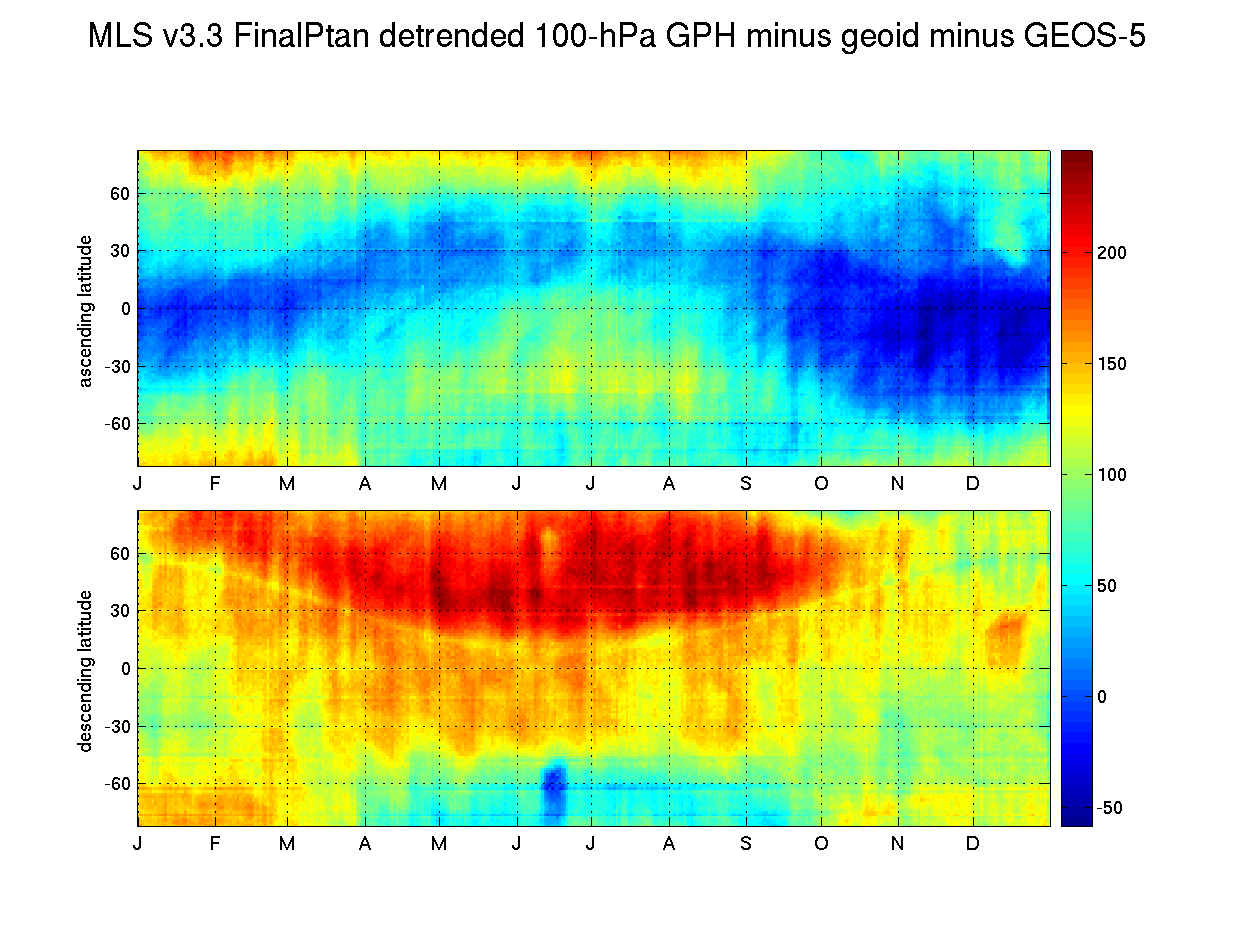
\includegraphics[width=0.7\linewidth]{figures/GPH_geoid_correction2A}
\caption{Annually-repeating biases between MLS 100-hPa GPH and GEOS-5.2
  100-hPa GPH as functions of ascending and descending latitude and of
  day of year.  These biases were computed based upon data from the
  years 2005--2012. (I will remake this figure as a native eps.)}
\label{fig:GPH_lat_annual}
\end{figure}
Some of this annually-repeating ``bias'' is likely annually-repeating
geophysical information captured by MLS that is not in the GEOS-5
analysis, but the large ascending-descending are almost certainly not
primarily diurnal effects.  After removal of this annually-repeating
bias and a there is a residual global decreasing trend in the MLS
100-hPa GPH relative to GEOS-5 of $\sim$100\,m in the first 4 years of
the mission, 2005--2008, with a further $\sim$15\,m decrease in
2009--2012.  The standard deviation of the differences between the
bias-corrected MLS and GEOS-5 100-hpa GPH is on the order of 20\,m.

\subsection*{Differences between \thisv and previous versions}

The \thisv GPH values are typically slightly higher than those of the
v3.3 product, with typical mean differences ranging from 20\,--\,40\,m
in the stratosphere, increasing by $\sim$10\,m in the upper troposphere
and in the mesosphere.  Typical scatter about the mean difference is
$\sim$40\,m at 100\,hPa, increaing to 60\,m at 1\,hPa and 100\,m at
0.01\,hPa.  Seasonal and latitudinal variations in the mean difference
between \thisv and v3.3 GPH are typically less than 20\,m, with somewhat
larger seasonal differences in the high southern latitudes and above
0.01\,hPa.  As with temperature, the 316-hPa level of \thisv GPH is not
recommended for scientific use.  The standard \thisv GPH product is
reported on the same 55-level grid as is the \thisv temperature.

\subsection*{Vertical resolution}

The GPH profile is vertically-integrated temperature, so its vertical
resolution is not well-defined.  The vertical resolution of the
underlying temperature given in Section~\ref{sec:StandardTemperature} is
repeated in Table~\ref{tab:GPHSummary}.

\subsection*{Precision}

MLS \thisv GPH precision is summarized in Table~\ref{tab:GPHSummary}.
Precision is the random component of measurements that will average-down
if a measurement is repeated.  The retrieval software returns an
estimate of GPH precision only for the 100\,hPa reference level, as this
is the only element included in the MLS ``state vector.''  GPH precision
at other standard-product profile levels (summarized in column~2 of
Table~\ref{tab:GPHSummary}) is calculated from the GPH precision at the
reference level and the profile of temperature precisions.  Calculated
precision values are \texttildelow35\,m from 261\,hPa to 100\,hPa,
\texttildelow45\,m at 1\,hPa, \texttildelow110\,m at 0.001\,hPa.
Off-diagonal elements of the temperature/GPH error covariance matrix are
neglected in this GPH-precision-profile calculation, but resulting
errors are believed to be small (\texttildelow5\,m near 100\,hPa.)

\subsection*{Accuracy}

The accuracy of the v2.2 GPH was modeled based upon consideration of a
variety of sources of systematic error, as discussed in
\citep{SchwartzEtal08}. \thisv accuracy is believed to be substantially
similar and the results of the v2.2 calculations are given in column
four of Table\,\ref{tab:GPHSummary}. Of the error sources considered,
modeled amplifier non-linearity had the largest impact, just as is the
case with the calculation for temperature.

The second terms in column four are model-based estimates of the bias
magnitude from other sources including uncertainty in
pointing/field-of-view, uncertainty in spectroscopic parameters, and
retrieval numerics.  The combined bias magnitudes due to these sources
is 100\,--\,150\,m.

``Observed bias uncertainty'' in Table~\ref{tab:GPHSummary} is an
estimate of bias based upon comparisons with analyses and with other
previously-validated satellite-based measurements.  These comparisons
were made using MLS v2.2, but as the biases between v2.2 and \thisv GPH
are generally less than 50\,m from 261\,--0.1\,hPa and reasonably
constant, so these results hold for \thisv as well.  The primary sources
of correlative data were the Goddard Earth Observing System, Version
5.0.1 data assimilation system (GEOS-5) \citep{ReineckerEtal07}, used in
the troposphere and lower stratosphere, and the Sounding of the
Atmosphere using Broadband Radiometry (SABER)
\citep{MlynczakAndRussell95}, used in the upper stratosphere through the
mesosphere.  MLS has a 150\,m high bias relative to analyses (GEOS-5) at
100-hPa that drops to 100\,m at 1\,hPa.  Biases with respect to SABER
are small at 0.1\,hPa but increasingly negative at higher levels,
reaching -600\,m at 0.001\,hPa, but with significant latitudinal and
seasonal variability.

\subsection*{Data screening}

GPH should be screened in the same way as is temperature:

\begin{description}
\item[Pressure range:] \screeningrule{261\,--\,0.001\,hPa.}
  \standardrangestatement

  \standardprecisionrule GPH precision is set negative at and beyond any
  level in the integration of temperature away from the 100-hPa
  reference level where temperature has negative precision.

\evenstatusrule

\item[Clouds:]

  \screeningrule{Thick clouds are believed have some impact on \thisv
    GPH measurements in the upper troposphere (261\,--\,100\,hPa),
    however the cloud-flags bits of the \thisv GPH status are not useful
    in screening out cloud impacts.  Screening of \thisv tropospheric
    GPH for values impacted by clouds is an area of ongoing research.}

\item[Quality:] \qualityrule{0.9} This threshold typically excludes
  1.4\% of global profiles, but 4.8\% of tropical profiles.

\item[Convergence:] \convergencerule{1.021} Use of this threshold
  typically discards 0.1\% of profiles and eliminates a significant
  fraction, but not all of a non-Gaussian tail of outliers that
  comprises less than 0.01\% of the 100-hPa retrieved values.

\end{description}

\subsection*{Review of comparisons with other data sets}
\label{sec:GPHComparisons}

The 100\,hPa reference GPH is typically 100\,--\,250\,m higher than
GEOS-5 in the northern high latitudes and 50\,--\,200\,m higher than
GEOS-5 in the Southern high latitudes. As GPH profiles are calculated
relative to the reference level, biases at 100\,hPa move entire profiles
up and down.  At low latitudes, the GPH observations taken on the
ascending branch of the orbit are typically 0\,--\,120\,m higher than
GEOS-5. while those from descending branch are 100\,--\,200\,m higher.
A seasonal cycle in the daily mean ascending/descending differences of
\texttildelow100\,m peak-to-peak is evident in the high-southern
latitudes (peaking in January) and in the ascending branch of the
equatorial mean differences (peaking in July) There has been a general
downward trend in the MLS minus GEOS-5 bias of 40\,--\,50\,m/year over
the life of the mission.  Like v2.2 GPH, \thisv GPH has a bias of
\texttildelow100\,m at 10\,hPa with respect to GEOS-5 and SABER, and the
bias with respect to SABER becomes increasingly negative at lower
pressures: \texttildelow\,$-$100\,m at 0.01\,hPa and
\texttildelow\,$-$500\,m at 0.001\,hPa.  These negative biases reflect
the general low temperature bias of MLS with respect to SABER.

\subsection*{Desired improvements for future data version(s)}

Reduction of biases in the GPH product likely requires improvement of
our ability to model atmospheric radiative transfer and/or the
measurement system to improve the fit between the forward model and
observed radiances near the O$_2$ spectral lines from which temperature
and pointing information are extracted.  The simple model of ``gain
compression'' proposed during v2.2 validation proved inadequate during
\thisv development, but research in this area is ongoing.  Some
seasonally and latitudinally-repeating systematic errors in GPH may be
the result of error in the absolute pointing reference that is taken
from the spacecraft attitude and ephemeris data stream.  Reduction of
these systematic errors is an area of ongoing research.
  
\begin{table}
\label{tab:GPHSummary}
\begin{minipage}{\linewidth}\small
\centering\begin{tabular}{cccccl}
\toprule
\textbf{Region} & 
\parbox[m]{22mm}{\centering\textbf{Resolution\\ \mbox{Vert. $\times$ Horiz.} / km}} &
\parbox[m]{18mm}{\centering\textbf{Precision\footnote{Precision on individual profiles} \\/ meters}} &
\parbox[m]{20mm}{\centering\textbf{Observed bias\\uncertainty\\ / m}} &
\textbf{Comments} \\
\midrule
$<$0.001\,hPa & --- & --- & --- & --- & Unsuitable for scientific use \\
0.001\,hPa          & 10--13 $\times$ 220  & $\pm$110 & $-$450 & \\
0.01\,hPa           & 8--12 $\times$ 185  & $\pm$85   & $-$100 & \\
0.1\,hPa            & 6 $\times$ 165   & $\pm$60   &  0  & \\
1\,hPa              & 7 $\times$ 165   & $\pm$45   & 100 & \\
10\,hPa             & 4.3 $\times$ 165 & $\pm$35   & 100 & \\
100\,hPa            & 5.2 $\times$ 165 & $\pm$30   & 150 & \\
261\,hPa            & 5.3 $\times$ 170 & $\pm$35   & 150 & \\
1000\,--\,316\,hPa & ---      & ---             & ---     & --- & Unsuitable for scientific use\\
\bottomrule
\end{tabular}
\end{minipage}
\end{table}

%%% Local Variables: 
%%% mode: latex
%%% TeX-master: "v4-x-report"
%%% End: 

\speciestitle{Water Vapor}{H\cs2O}{H2O}{
\item[Useful range:] 316\,--\,0.001\,hPa
\item[Contact:] Alyn Lambert (stratosphere/mesosphere),
  \email{alyn.lambert@jpl.nasa.gov} \\
  William Read (troposphere), \email{william.g.read@jpl.nasa.gov}}

\subsection{Introduction}

The standard water vapor product is taken from the 190-GHz
``\texttt{CorePlusR2}'' retrieval. The vertical grid for H\cs2O is: 12
levels per decade change in pressure (LPD) for 1000\,--\,1 hPa, 6\,LPD
for 1.0\,--\,0.1\,hPa, and 3\,LPD for 0.1\,--\,10\cp{$-$5}\,hPa. The
horizontal grid is every 1.5\degsym along the orbit track.  H\cs2O is
unusual among MLS products in that it is assumed that the logarithm of
the volume mixing ratio (VMR), and not mixing ratio itself, varies linearly
with log pressure; however, H\cs2O, like the other MLS constituents is
retrieved in VMR (not $\log$ VMR). Vertical and horizontal interpolations of
H\cs2O should be performed linearly on the logarithm of the H\cs2O
concentration (VMR). The concentration of H\cs2O in the MLS files are unitless,
VMR, in the Level 2 Geophysical Product (L2GP) files; however, its
concentration is quite low in the upper atmosphere and it is more convenient
to express its concentration in parts per million volume (ppmv =
VMR$\times 10^{6}$), a unit commonly used to describe its features in this
section. The recommended vertical range is 316\,--\,0.001\,hPa (height
indicies, 7--49, starting at 1). The uppermost retrieved level 0.00046\,hPa
(height index 50) is not vertically resolved from the levels above it and is
more like a column measurement but may be usable for some studies. The MLS
science team should be consulted prior to using data from 0.00046~hPa level.

The MLS \thisv H\cs2O between 1000 and 383\,hPa is taken from a
retrieval of relative humidity with respect to ice (RHi) product,
converted to specific humidity using the Goff-Gratch vapor pressure over
ice equation.  This RHi retrieval is not vertically resolved, and all
levels between 1000 and 383\,hPa are assumed to have the same RHi.  See
Section~\ref{sec:StandardRHI} for more information. H\cs2O for
p$\le$0.000215\,hPa are filled with \emph{a priori} values. Validation of MLS
v2.2 water vapor is presented in \citet{ReadEtal:2007} and
\citet{LambertEtal:2007}.  This section reiterates the key information from
those studies, and updates them for \thisv.  Table~\ref{tab:H2OSummary}
gives a summary of MLS \thisv H\cs2O precision, resolution, and accuracy.

\subsection{Changes from \prevv}

A defect in \prevv and prior versions is that MLS exhibits a rather
low bias (20--50\%) at 2-3 km below the tropopause [Read et al in prep, 2020].
Another feature is that MLS shows a very small seasonal cycle at 147~hPa in
the tropics. The two issues are related. The tropopause height has a strong
seasonal cycle in the tropics and therefore the dry bias at a given height
will be modulated accordingly and acted to flatten the seasonal cycle at
147~hPa. Another issue is that the MLS H\cs2O measurement is drifting due
to aging of the instrument. A possible drift in the MLS H\cs2O was first noted
by \citet{HurstEtal:2016}. After an in depth investigation into possible
causes behind these issues, a most likely contributor is a combination of a
sideband fraction characterization error and a radiometer pointing error.
The center channels in the radiometer band (B2) that is dedicated to
measuring H\cs2O are opaque while the instrument FOV scans the stratosphere and
provides a temperature measurement of the stratosphere. Long term measurements
show an unexpected offset relative to what we believe is the stratospheric
temperature is and also shows a drift. Assuming that the stratospheric
temperature is known (available from the 118~GHz radiometer) and is not
drifting apart from atmospheric changes, then a new sideband fraction and
drift can be charaterized from the opaque channels in B2. The analysis
suggests that 190 GHz radiometer lower sideband fraction is 6.85\% too low
and has drifted ~1\% during the mission lifetime. Implementing these changes
helped resolve another inconsistency we had with the 190~GHz. Using the H\cs2O
linewidth to retrieve pointing e.g. tangent pressure, differed from that from
the 118~GHz radiometer which uses O\cs2 by 250m. Applying the sideband
correction reduced this inconsistency to 70m which is within the measured
uncertainty of the radiometer pointing alignment among the different
radiometers. Therefore a 70m adjustment to the radiometer alignment is
applied. With these adjustments
the retrieved ptan from the 190~GHz (CorePlusR2) is now consistent within ~20m
of that retrieved from the 118 and 240~GHz (CorePlusR3) and is retrieved
operationally now. These changes have helped to mitigate the large dry bias
2--3~km below the tropopause and consequently, increased the seasonal cycle
of the 147~hPa H\cs2O in the tropics. These changes have helped to reduce
biases and drifts between the 190~GHz and the standard product ozones.

Another improvement to the H\cs2O retrieval is using a line by line radiative
transfer model to calculate radiances for the digital autocorrelator channels
(128, 100~kHz channels centered on the H\cs2O line) instead of using a
linear approximation of the model. This change will properly account for non
linearities in the signal dependence on the H\cs2O concentration. Some
adjustments were made to the \emph{a priori} precision and smoothing to
produce positive precisions and potentially make
the product useful up to 0.001~hPa. The retreival range for H\cs2O
is raised to 0.00046~hPa in \thisv.

The median daily quality for v4.2 declined by 4.8\% from 2010 to 2020. The
decline follows a declining trend in the radiometer system temperature that
determines the measurement signal noise that is also declining making the
goodness of fits degrade slightly. In \thisv, the decline over the same ten
year period is only 0.8\% due to incorporating a tangent pressure retrieval.

\begin{figure}
\begin{center}
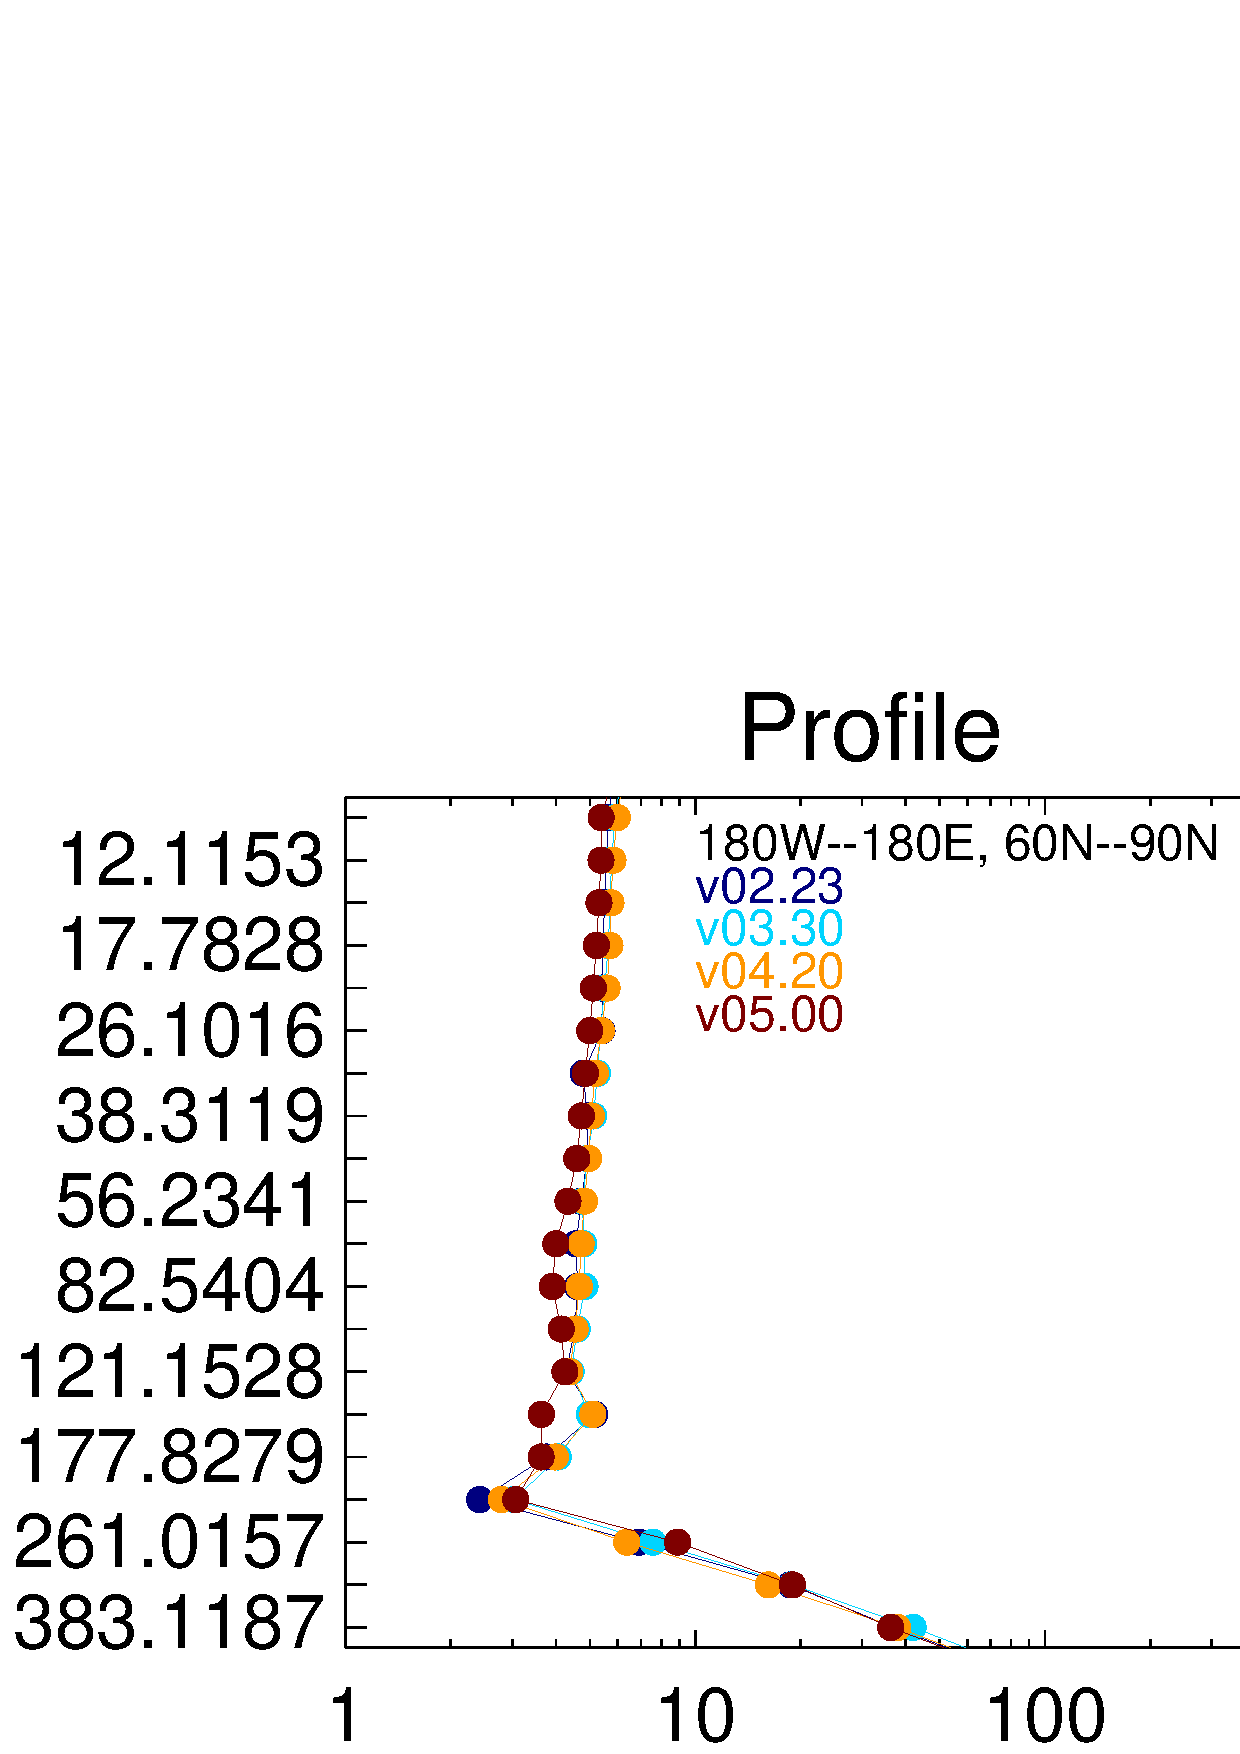
\includegraphics[width=0.8\linewidth]{figures/mls_h2o_v2-v3-v4-v5_prfl_comp_60n-90n}
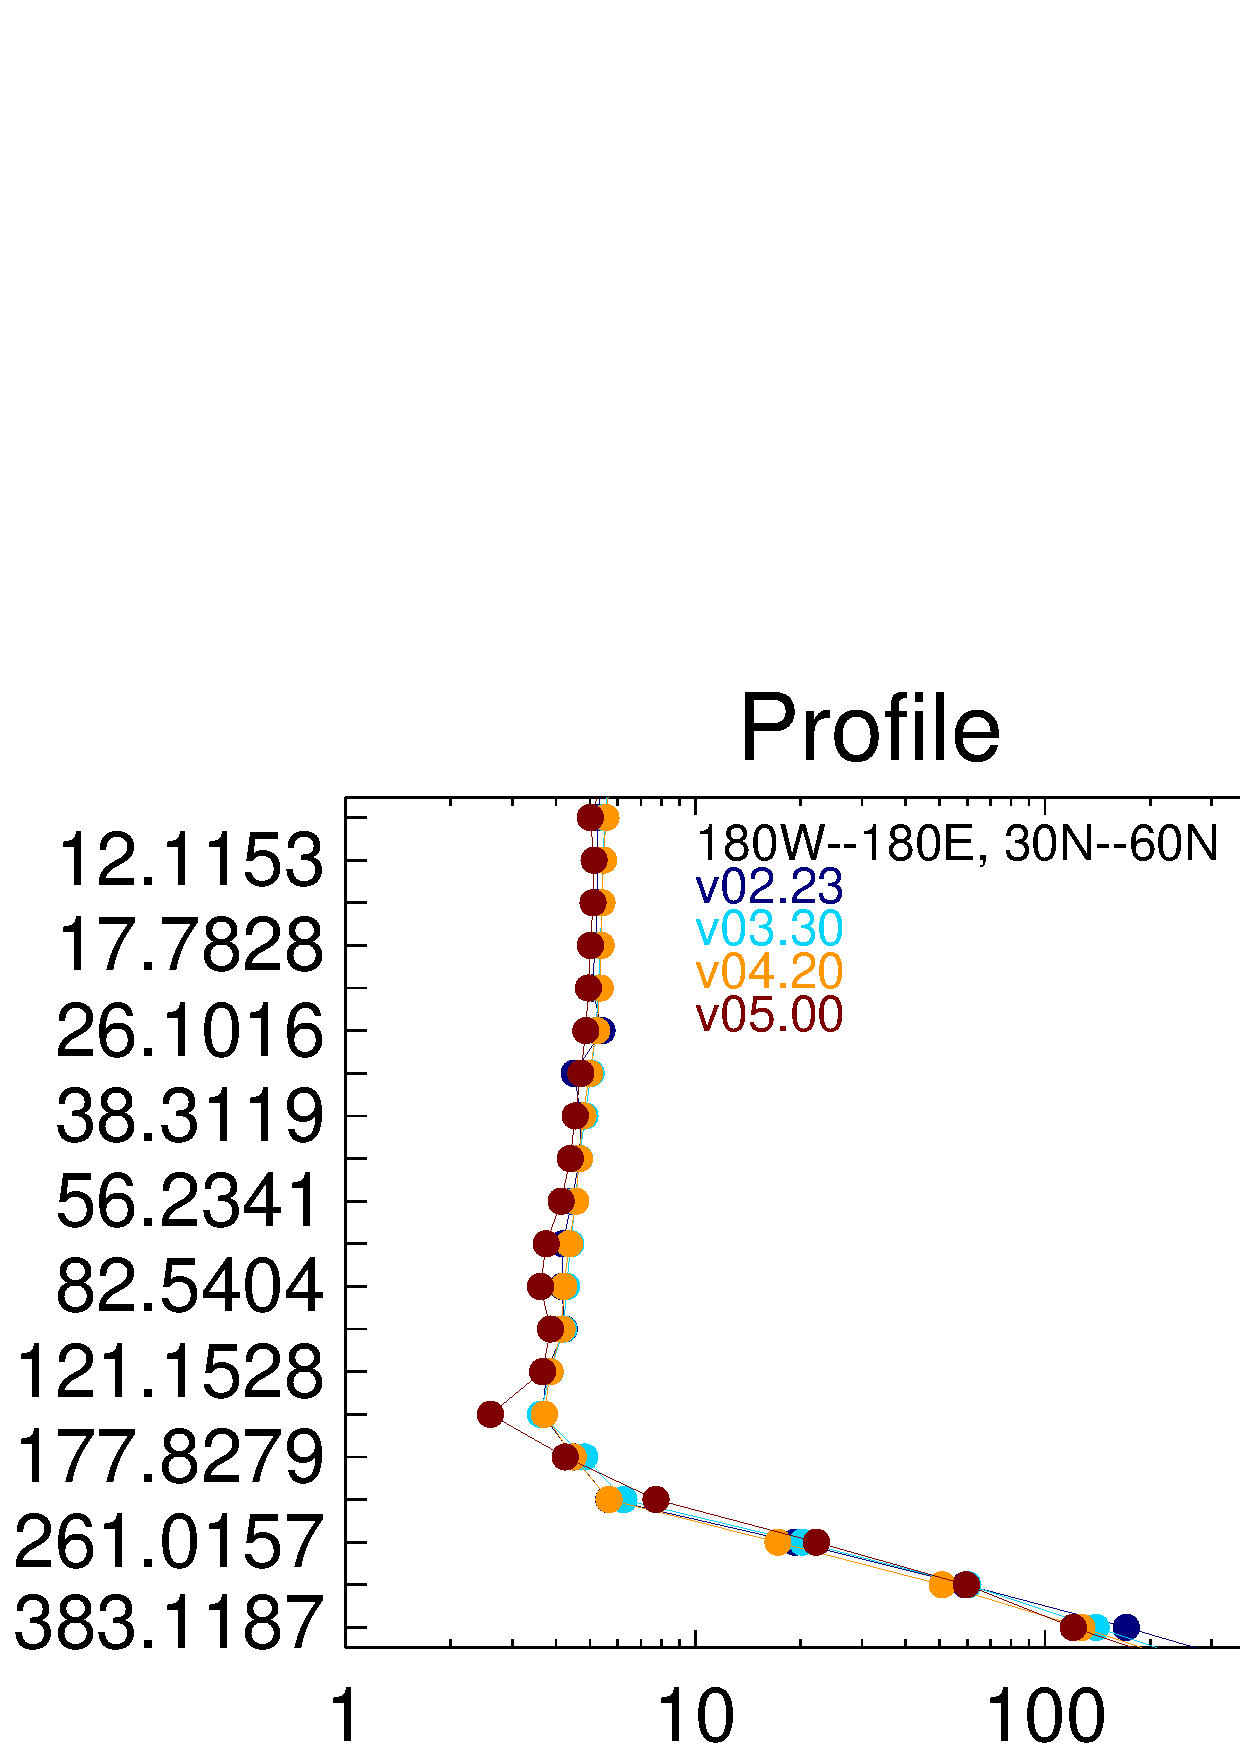
\includegraphics[width=0.8\linewidth]{figures/mls_h2o_v2-v3-v4-v5_prfl_comp_30n-60n}
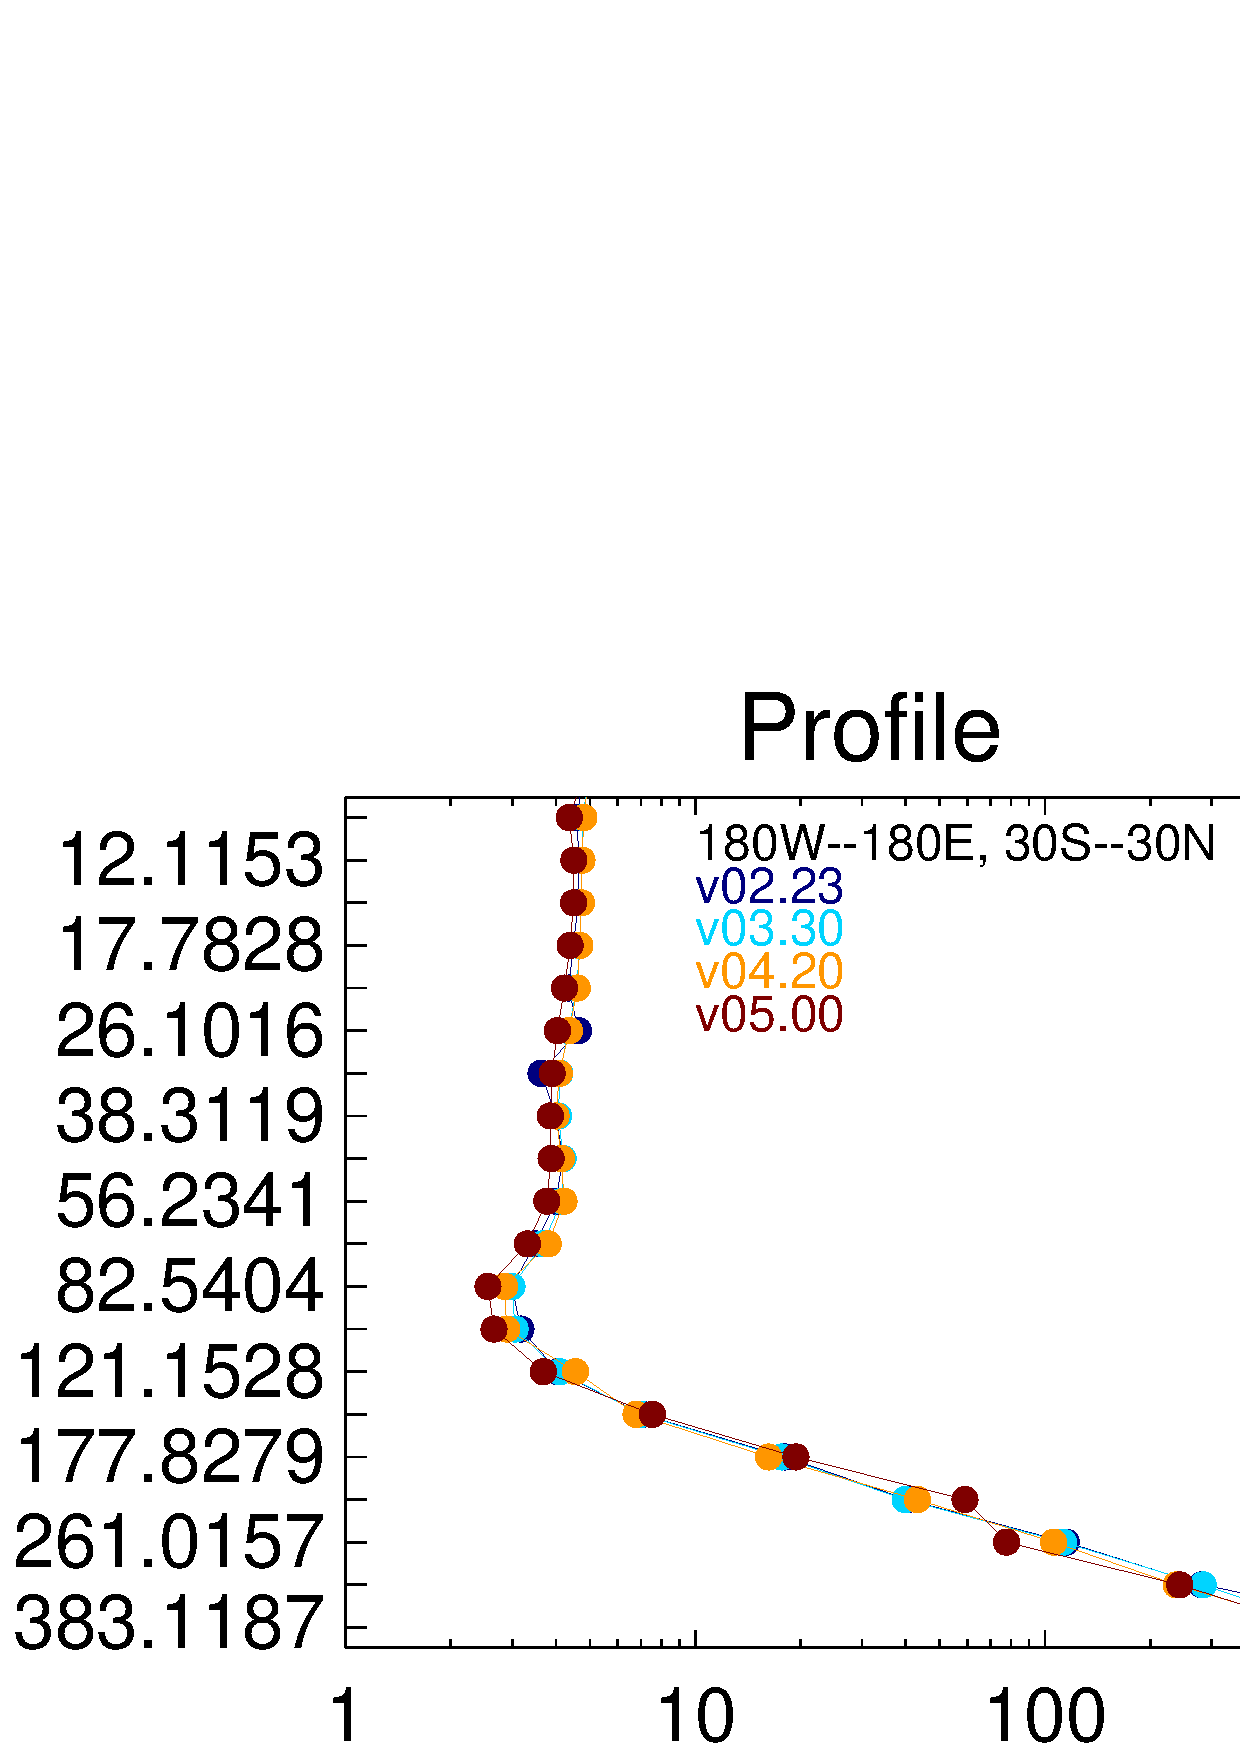
\includegraphics[width=0.8\linewidth]{figures/mls_h2o_v2-v3-v4-v5_prfl_comp_30s-30n}
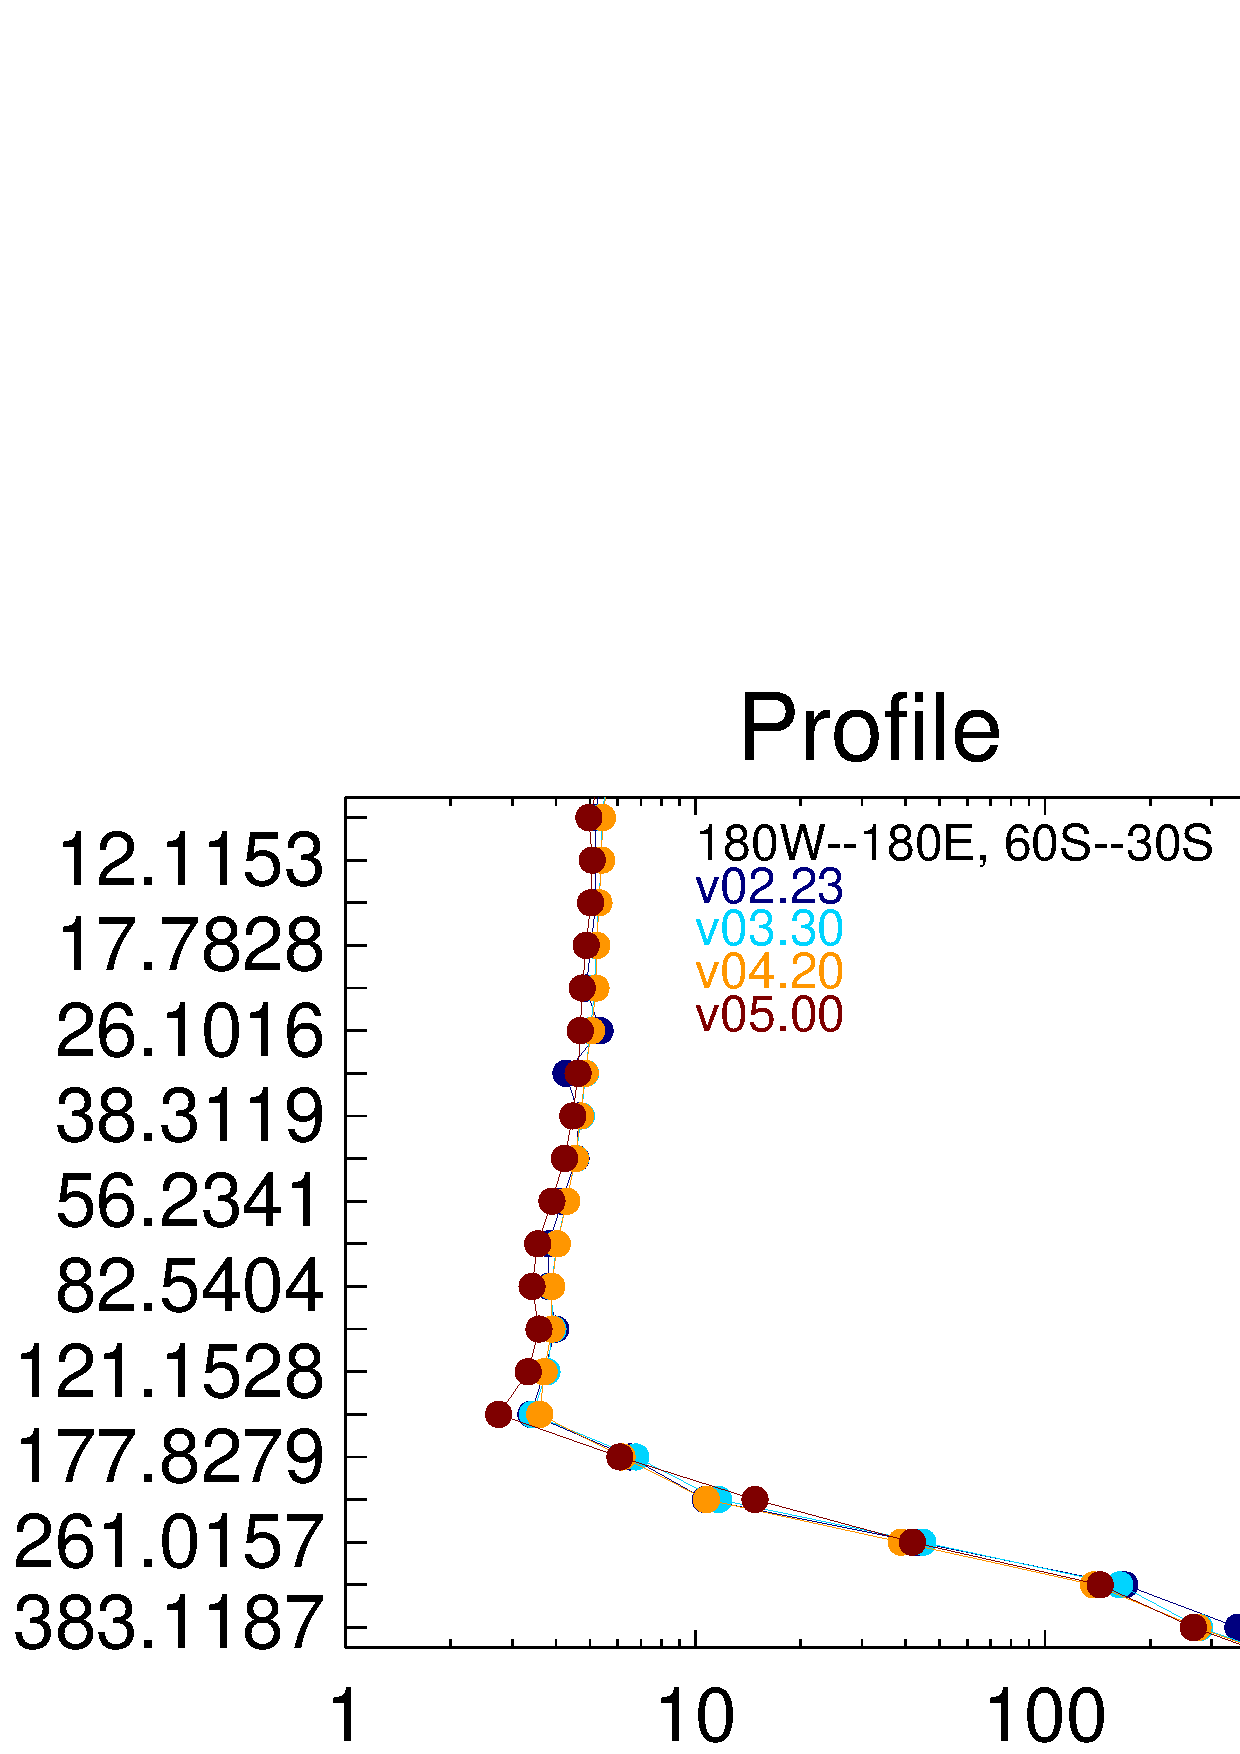
\includegraphics[width=0.8\linewidth]{figures/mls_h2o_v2-v3-v4-v5_prfl_comp_60s-30s}
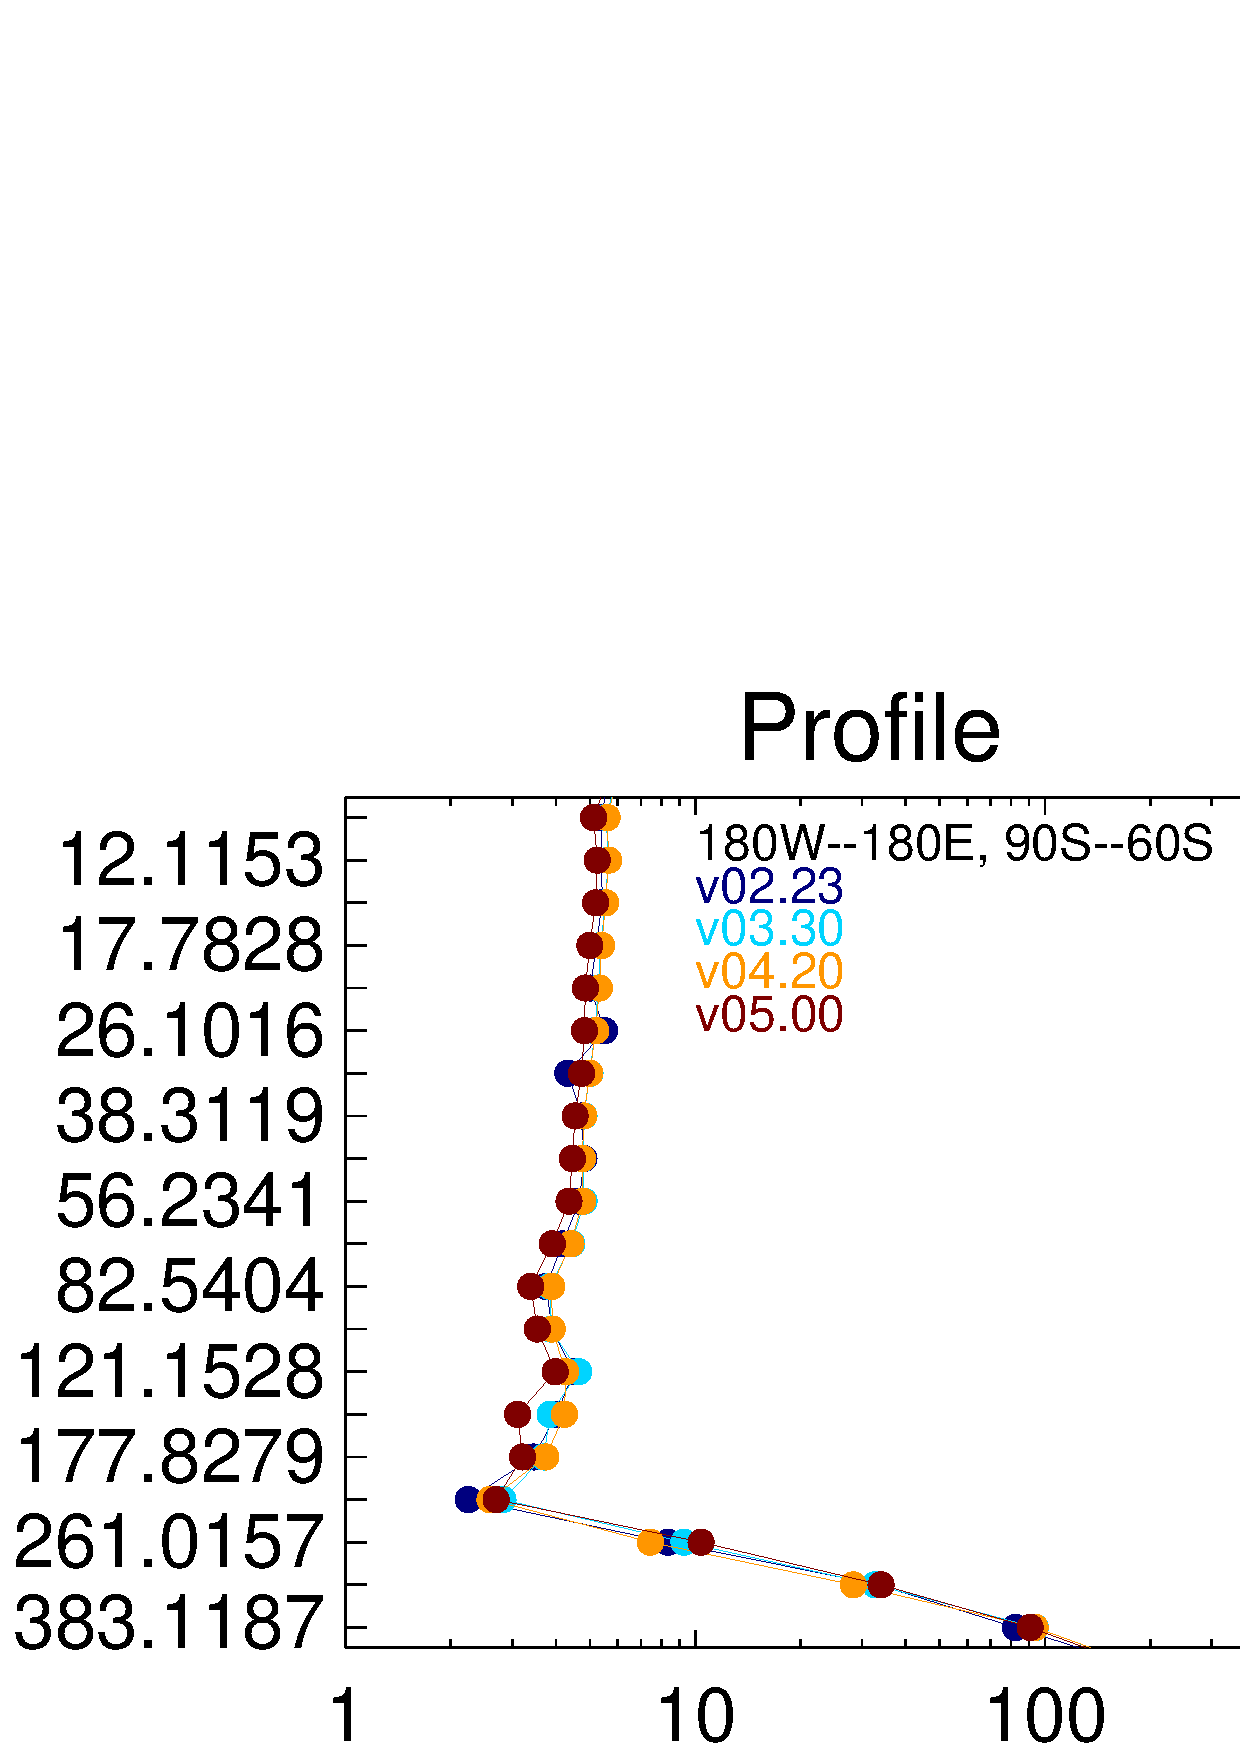
\includegraphics[width=0.8\linewidth]{figures/mls_h2o_v2-v3-v4-v5_prfl_comp_90s-60s}
\end{center}
\caption{A comparison of v2.23(blue), v3.30 (cyan), v4.20 (orange), and
  v5.00 (red) water vapor for Jan-Feb-Mar 2009 in 5 latitude bands. Other time
  periods are similar. The left panel compares mean profiles, the center
  shows the mean difference (red and green diamonds) surrounded by each
  version's estimated precision, and the right panel shows the estimated
  retrieval precision (solid and bullets), measured variability
  (dotted),  which includes atmospheric variability about the mean, and the
  \emph{a priori} precision (dashed and diamonds) profile.}
\label{fig:avgmlsprflcomptropstrat}
\end{figure}

Figure~\ref{fig:avgmlsprflcomptropstrat} compares MLS \thisv to all previous
versions starting with v2.2. The differenes are with respect to v2 which is
the product the validation paper was written about. Notable differences are
the removal of a kink in v2.2 at 32/26~hPa beginning with v3.3 caused by a
linewidth error and extending a finer grid, 12 lpd versus 6, above 22~hPa
to 1~hPa. Version 4.2 saw improvements in cloud screening and in the lower
resolution initial H\cs2O phase that is used to
initiallize values and profile shape smoothing for the final high resolution
phase. These changes improved agreement with similated data at the
316--215~hPa levels. The change in sideband fraction in v5 leads to a 5--10\%
reduction in H\cs2O in the stratosphere and above. The change in pointing
also caused by the sideband fraction change and the new estimate of the
radiometer pointing offset causes a moistening of the levels 2~km below the
tropopause. Nominally this is 147~hPa in the tropics, 215~hPa at mid-latitudes
and 261~hPa at high latitudes. The extremely low values retrieved at 215~hPa
at high latitudes seen in previous versions appear to be less dry in v5.

The handling of humidity data at pressures greater than 316\,hPa is
unchanged from v4. Text describing those changes in the v4 quality document
is repeated here. Humidity data at pressures greater
than 316\,hPa are derived from a
broad layer relative humidity retrieval (using low limb viewing MLS wing
channel radiances) similar to that obtained from NOAA operational
humidity sounders such as TOVS\@. As noted in \citep{ReadEtal:2007}, the
v2.2 retrieval at pressures larger than 316\,hPa was likely to be
\texttildelow30\% too high, based on comparisons with AIRS\@. The
accuracy of this retrieval is highly sensitive to the transmission
efficiency of the MLS optics system. In \prevv the assumed value of the
MLS antenna transmission efficiency was adjusted empirically (within the
uncertainty range established from MLS calibration) to give better
agreement with AIRS in the tropics. In \thisv the N\cs2 continuum was
adjusted only for this phase to minimize the clear sky cloud induced
radiance bias. This retrieval is used as an \emph{a priori} and profile
constraint for the humidity profile at pressures greater than 316\,hPa,
which are not retrieved in the standard H\cs2O product retrieval.

\sloppypar The third panel in Figure~\ref{fig:avgmlsprflcomptropstrat}
shows the mean
estimated single profile precision and the measured variability (which
includes instrument noise and atmospheric variability). The estimated
precisions are similar for most heights except up high 0.0046--0.00046~hPa
where the smoothing and uppermost retrieval level was changed and raised
respectively and in the upper troposphere where the estimated precision
roughly scales by the amount of H\cs2O. Higher concentrations of H\cs2O are
typically accompainied with higher values of precision. Because of the large
dynamic range of possible humidity in the upper troposphere and the non-linear
behavior of the instrument response to these concentrations is why H\cs2O
basis representation uses logarithm of concentration. Version 2
used a more coarse retrieval grid above 22\,hPa and a different value of
the H\cs2O linewidth.  Together these account for H\cs2O precision
differences at these altitudes between v2 and later versions.

\begin{figure}
\begin{center}
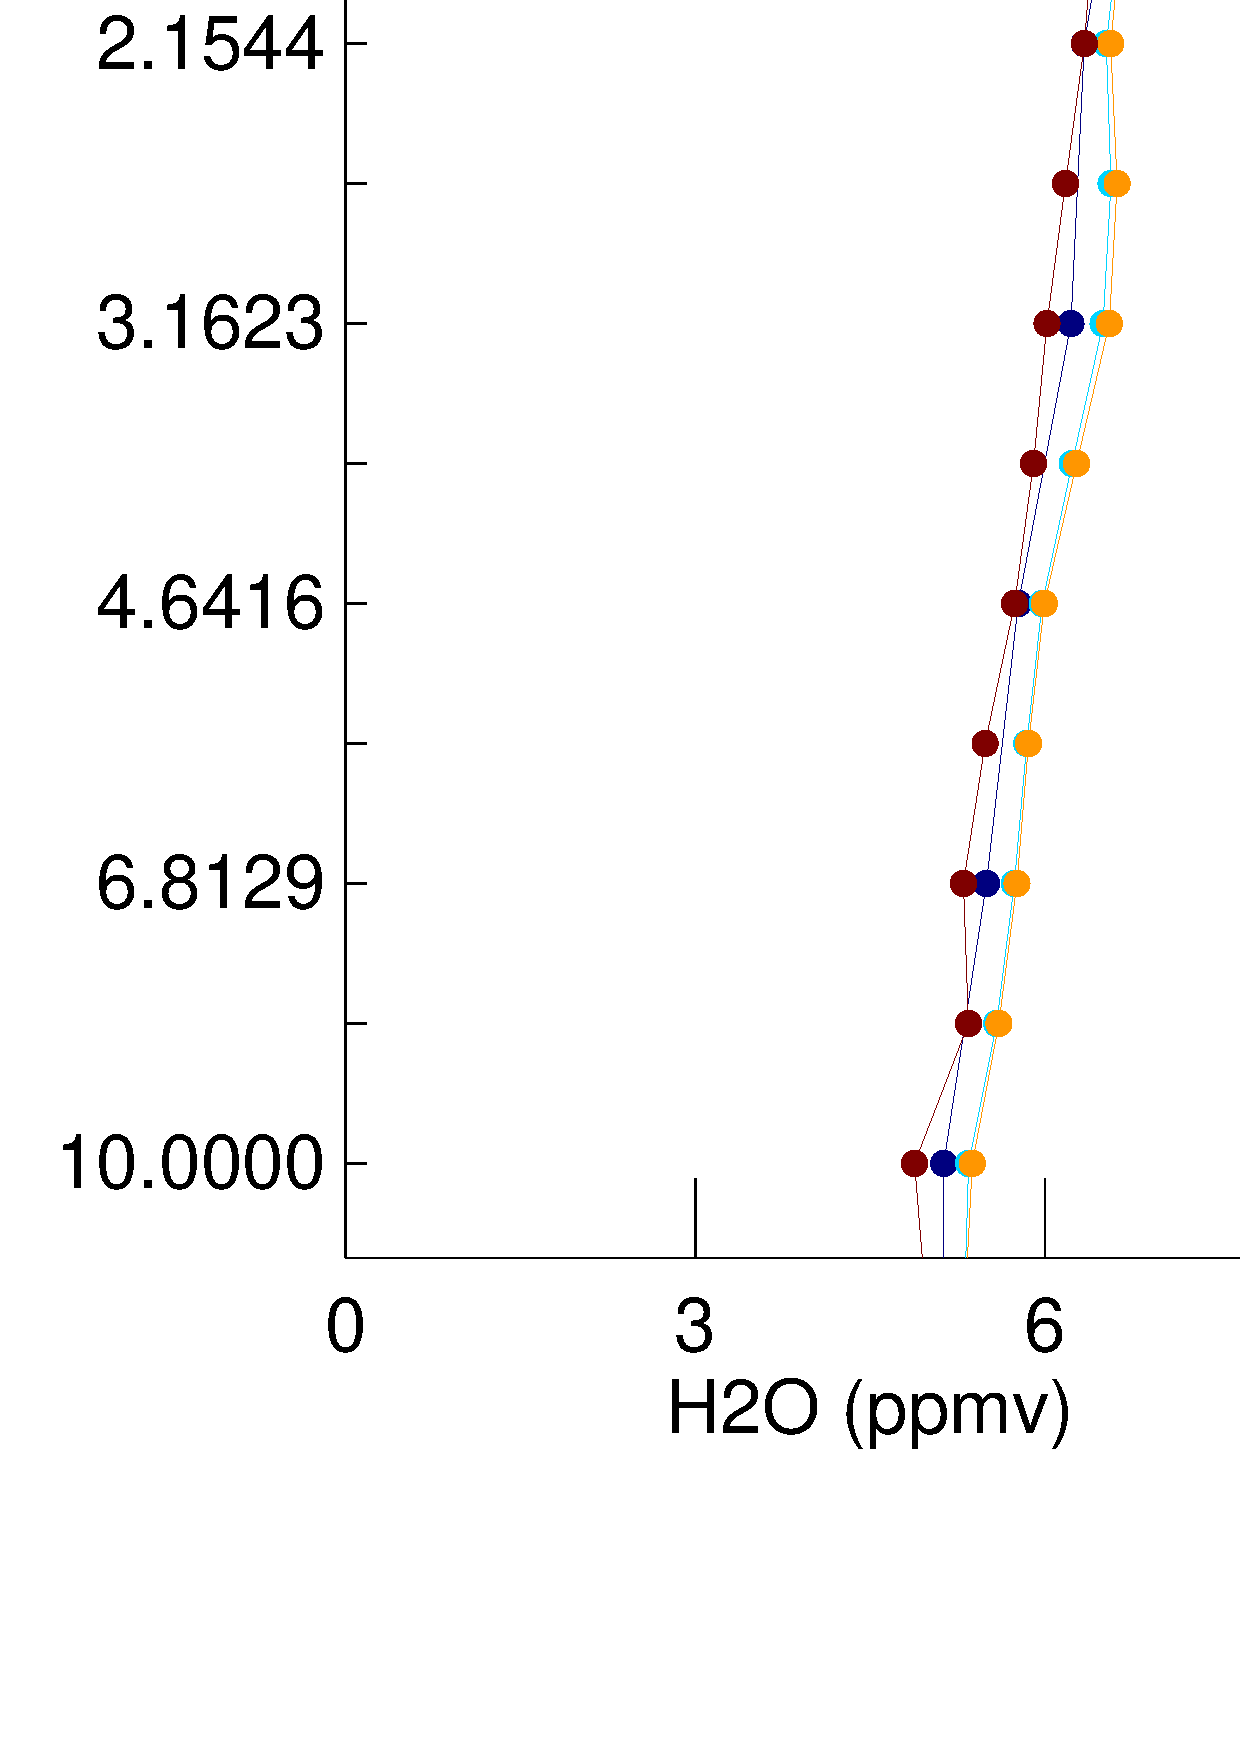
\includegraphics[width=0.8\linewidth]{figures/mls_h2o_v2-v3-v4-v5_prfl_comp_90s-90n_stratmeso}
\end{center}
\caption{An all-latitudes comparison of v2.23(blue), v3.30 (cyan), v4.20
  (orange), and v5.00 (red) water vapor for Jan-Feb-Mar 2009 showing levels
  in the middle stratosphere up to the mesosphere. Other time
  periods are similar. The left panel compares mean profiles, the center
  shows the mean difference (red and green diamonds) surrounded by each
  version's estimated precision, and the right panel shows the estimated
  retrieval precision (solid and bullets), measured variability
  (dotted),  which includes atmospheric variability about the mean, and the
  \emph{a priori} precision (dashed and diamonds) profile.}
\label{fig:avgmlsprflcompstratmeso}
\end{figure}

Figure~\ref{fig:avgmlsprflcompstratmeso} compares all versions beginning
with v02.2 to \thisv from 10~hPa to 0.0001~hPa. As expected, H\cs2O from
\thisv is lower than the other versions except v2 which had an erroneous
linewidth. Also shown is the increased \emph{a priori} precision being used
for \thisv for pressures lower than 0.0046~hPa in order to make the 0.001 and
0.00046~hPa levels usable. Using a non-linear radiative transfer model in
\thisv in place of an approximate linear model for the highly spectrally
resolved digital autocorrelator spectrometer (DACS) leads to some biases
in the uppermost levels. It is believed that
the better model being used for \thisv will produce more accurate results.

Figures~\ref{fig:avgmlsh2ozmcomp1} and \ref{fig:avgmlsh2ozmcomp2} show a
comparison of H\cs2O zonal means from v2, v3, v4, and v5 retrievals for
316\,--\,8.3\,hPa and 6.8\,--\,0.00046-hPa, respectively. In the stratosphere
v5 is usually lower than the previous versions due to the sideband adjustment.
Version 5 also shows a moist 147~hPa humidity in the tropics that becomes
a more moist 215~hPa at mid latitudes finalizing with a more moist 261~hPa at
high latitudes. In the mesosphere P$<$1~hPa, V5 is usually lower than the
previous versions but show similar structure until the top level
0.0005 (0.00046)~hPa where all other versions return the \emph{a priori},
but is actually a retrieved level in v5.

\begin{figure}
\begin{center}
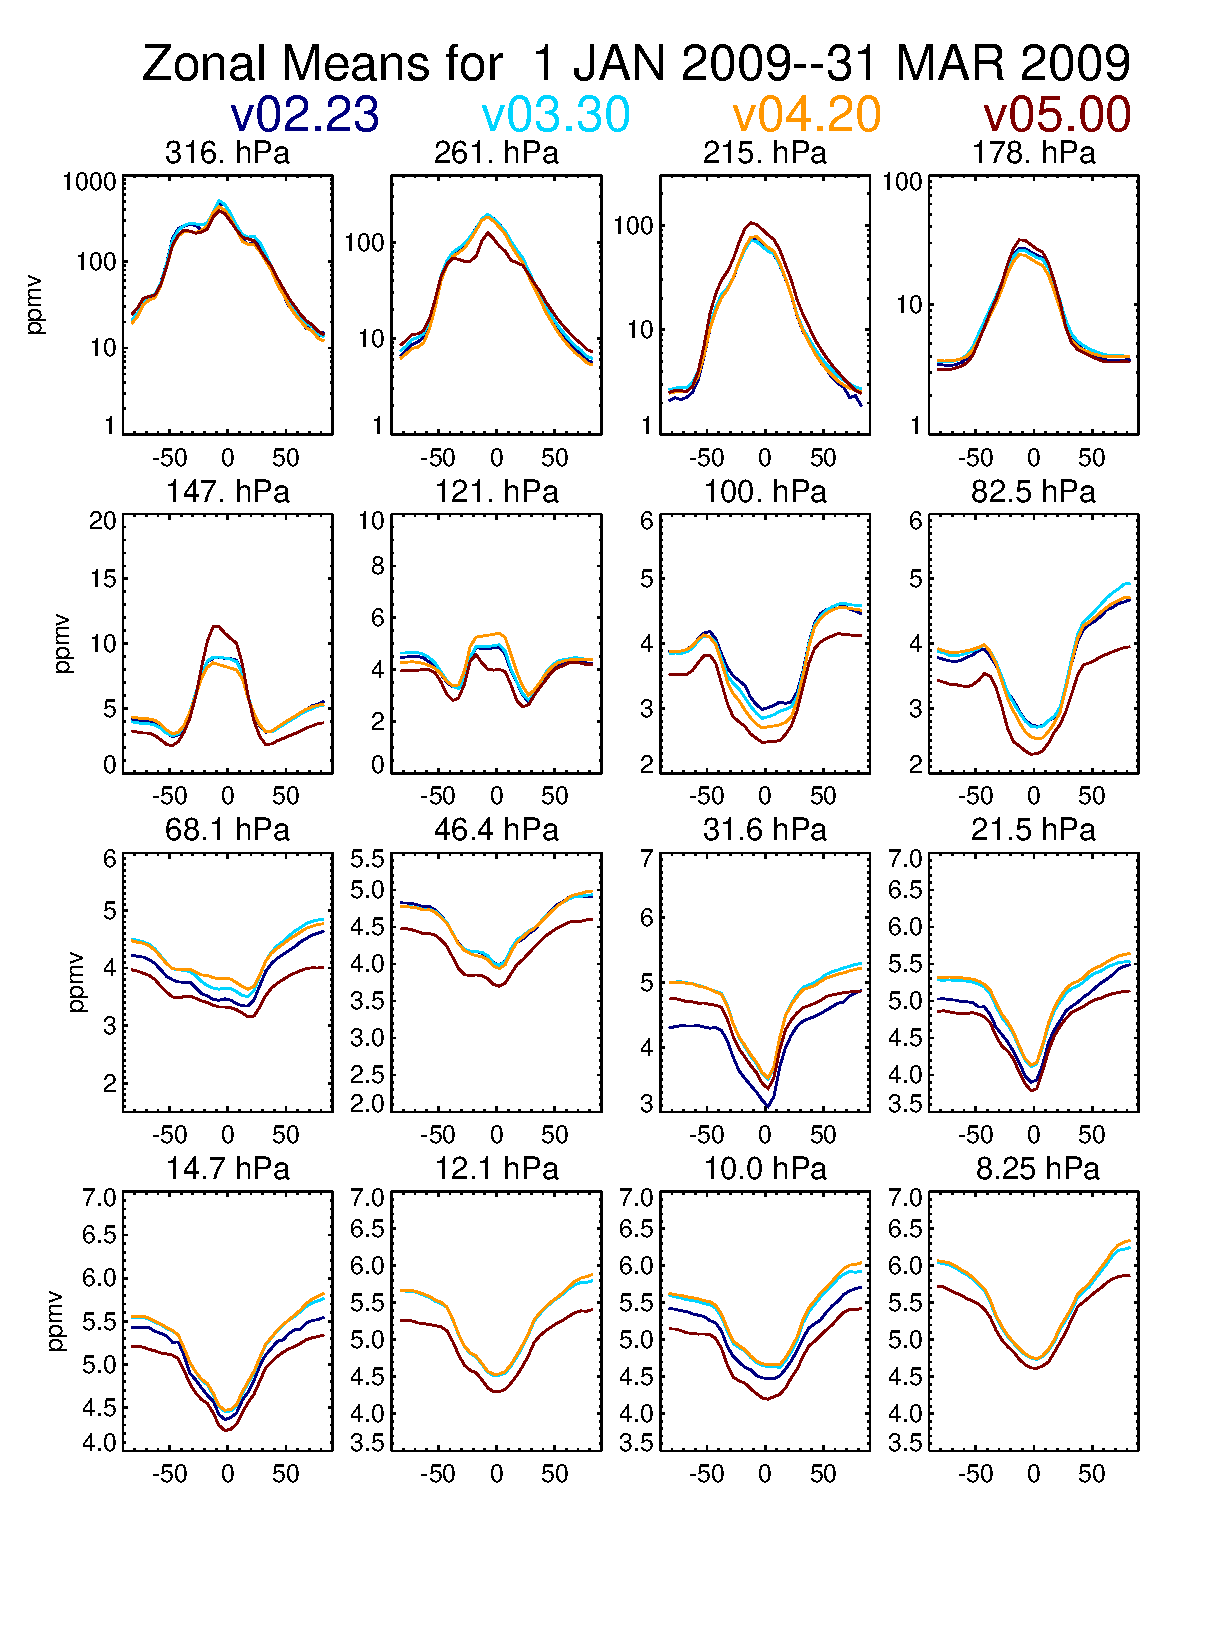
\includegraphics[width=0.8\linewidth]{figures/mls_h2o_v2-v3-v4-v5_zonal_means_ut-st}
\end{center}
\caption{A comparison of v2.23 (blue), v3.30 (cyan), v4.20 (orange), and v5.00
  (red), water vapor zonal means for Jan-Feb-Mar 2009. Each panel represents a
  pressure as noted above. The pressures shown range from 316~hPa to 8.3~hPa.}
\label{fig:avgmlsh2ozmcomp1}
\end{figure}

\begin{figure}
\begin{center}
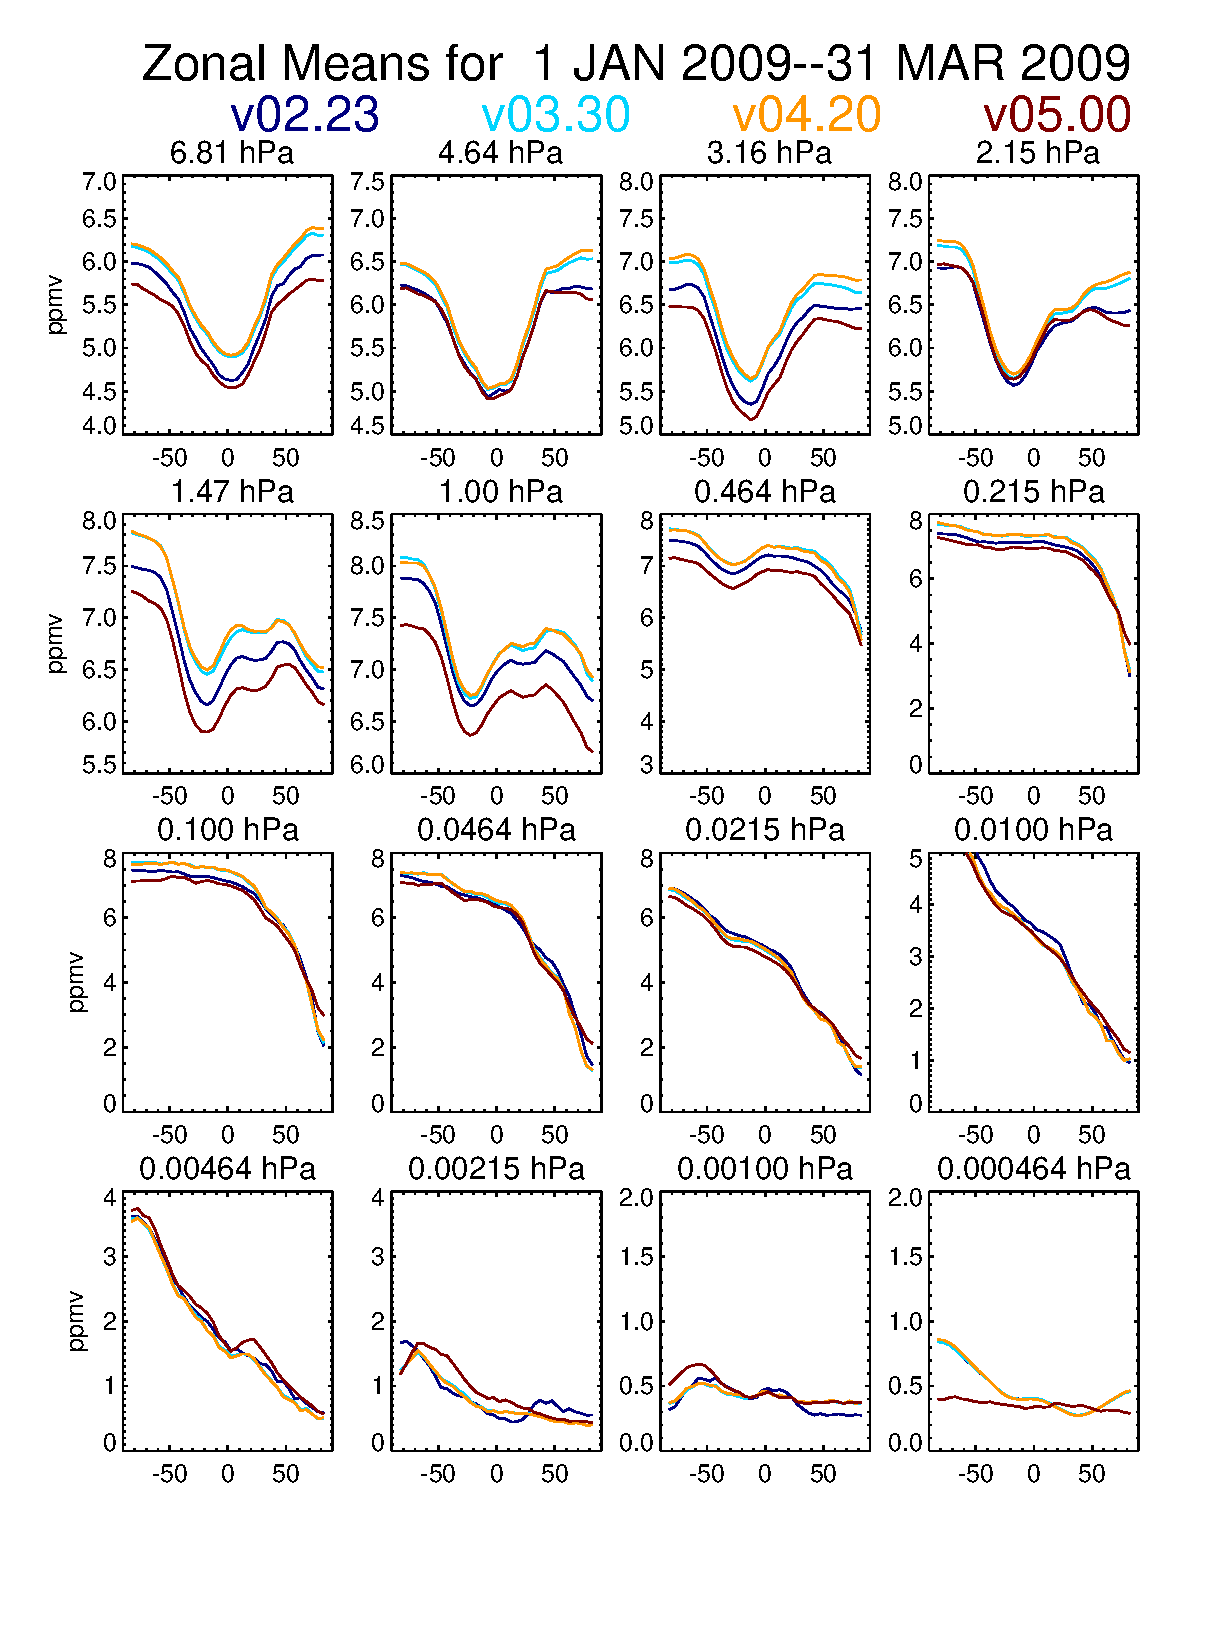
\includegraphics[width=0.8\linewidth]{figures/mls_h2o_v2-v3-v4-v5_zonal_means_usm}
\end{center}
\caption{A comparison of v2.23 (blue), v3.30 (cyan), v4.20 (orange), and v5.00
 (red) water vapor zonal means for Jan-Feb-Mar 2009. Each panel represents a
 pressure as noted above. The pressures shown range from 6.8\,hPa to
 0.00046\,hPa.}
\label{fig:avgmlsh2ozmcomp2}
\end{figure}

\subsection{Resolution}
\onestandardavk{H2O_HR}{H\cs2O}%

The spatial resolution is obtained from examination of the averaging
kernel matrices shown in Figure~\ref{fig:AvkH2O_HR}.  The vertical
resolution for H\cs2O is in the range 1.3\,--\,3.6\,km from
316\,--\,0.22\,hPa and degrades to 6\,--\,11\,km for pressures lower
than 0.22\,hPa. The along track horizontal resolution is
\texttildelow170\,--\,350\,km for pressures greater than 4.6\,hPa, and
degrades to 400\,--\,740\,km at smaller pressures. The resolutions in
Table~\ref{tab:H2OSummary} are a smoothed average of the equatorial and
70\degsym N values shown in Figure~\ref{fig:AvkH2O_HR}. The horizontal
cross-track resolution is 7\,km, the width of the MLS 190-GHz
field-of-view for all pressures. The longitudinal separation of the MLS
measurements is 10\degsym\,--\,20\degsym\ over middle and lower
latitudes, with much finer sampling in polar regions. The instrument
nominally scans to 0.001~hPa, therefore the retrieved value at 0.00046~hPa
is not vertically resolved and is effectively a column measurement from
0.001~hPa to the spacecraft with the H\cs2O profile values for
p $\le$ 0.000215~hPa fixed at \emph{a priori} values. The measurement
is only horizontally resolved.

\subsection{Precision}

Table~\ref{tab:H2OSummary} summarizes the estimated precision of the MLS
\thisv H\cs2O data. For pressures $\geq100$\,hPa, the precisions
given are the $1\sigma$ scatter about the mean of coincident comparison
differences, which are larger than the formal retrieval precisions
\citep{ReadEtal:2007}.  For pressures $\leq83$\,hPa the precisions are the
$1\sigma$ scatter of coincident ascending/descending MLS profile
differences \citep{LambertEtal:2007}.  The individual Level~2 precisions
are set to negative values or zero in situations when the retrieved
precision is larger than 50\% of the a priori precision -- an indication
that the data are biased toward the a priori value.

\subsection{Accuracy}

The values for accuracy are based primarily on two sources: comparisons
with validated instruments and a full systematic error analysis
performed on the MLS measurement system as described (for v2, but the
same approach will be used for \thisv) in \citet{ReadEtal:2007} and
\citet{LambertEtal:2007}. The results in Table~\ref{tab:H2OSummary}
are for \prevv because the analysis for \thisv is yet to be done; however,
it is expected that those for \thisv will be similar.
For pressures between 316\,--\,178\,hPa,
comparisons between AIRS v6 and MLS \thisv show $<20$\% agreement in the
zonal mean (MLS usually drier for low concentrations and wetter for high
concentrations) equatorward of 40\degsym\ with MLS having a dry
biases at higher latitudes.

The values in Table~\ref{tab:H2OSummary} for pressures between 316 and
178\,hPa are AIRS validated accuracies which are better than those
theoretically possible for the MLS measurement system. For the pressure
range 178\,--\,83\,hPa, the quoted values come directly from the
systematic error analysis performed on the MLS measurement
system. Comparisons between MLS and frost point hygrometers show that,
for the \prevv, when the tropopause is between 215 and 147\,hPa, MLS H\cs2O
2--3~km below the tropopause tends to have a large (20\,--\,40\%) dry bias.
It is anticipated that this dry bias will be reduced in \thisv but has yet
to be quantified. An estimate of the
accuracy between 121\,--\,83\,hPa is also from the systematic error
analysis performed on the MLS measurement system.  Comparisons among
\emph{in situ} sensors on the WB-57 high altitude aircraft and
frostpoint hygrometers flown on balloons show 30\% disagreements -- well
in excess of the estimated accuracy of each instrument including MLS --
near the tropopause and lower stratosphere.  The balloon based frost
point hygrometer shows agreement better than indicated in
Table~\ref{tab:H2OSummary}. The validation paper describes in detail why
a 30\% spread is inconsistent with the MLS measurements
\citep{ReadEtal:2007}.  For pressures less than 83\,hPa, the accuracy is
based on the systematic error analysis.

A long term drift in H\cs2O is being addressed in \thisv. It is believed
that a drift in the instrument sideband fraction is the cause and based on
opaque signals in the 190~GHz radiometer, can be evaluated and corrected.
More investigation will be done in the future to assess its performance.

\subsection{A note about the water vapor averaging kernels}

The averaging kernels are most applicable to linear and moderately
non-linear retrieval problems. The MLS H\cs2O retrievals are mostly
linear, except when the atmosphere approaches opaqueness. This occurs
when the limb tangent of the instrument field of view is less than
10\,km above the Earth's surface and the atmosphere is moist.  In such
cases the measurements are very nonlinear and often times the averaging
kernel calculations for the lowest retrieved levels are numerically
unstable, and unrepresentative of the actual MLS measurement system.
This is the case, for example, for the 316-hPa and 262-hPa equatorial
kernels shown in Figure~\ref{fig:AvkH2O_HR}.  Analysis of simulated MLS
observations indicates that application of the averaging kernel provides
little benefit to analyses involving the 316-hPa and 262-hPa levels, and
accordingly we recommend not applying the (unrepresentative) kernels at
those levels.

\subsection{Review of comparisons with other datasets}

\begin{figure}
\begin{center}
  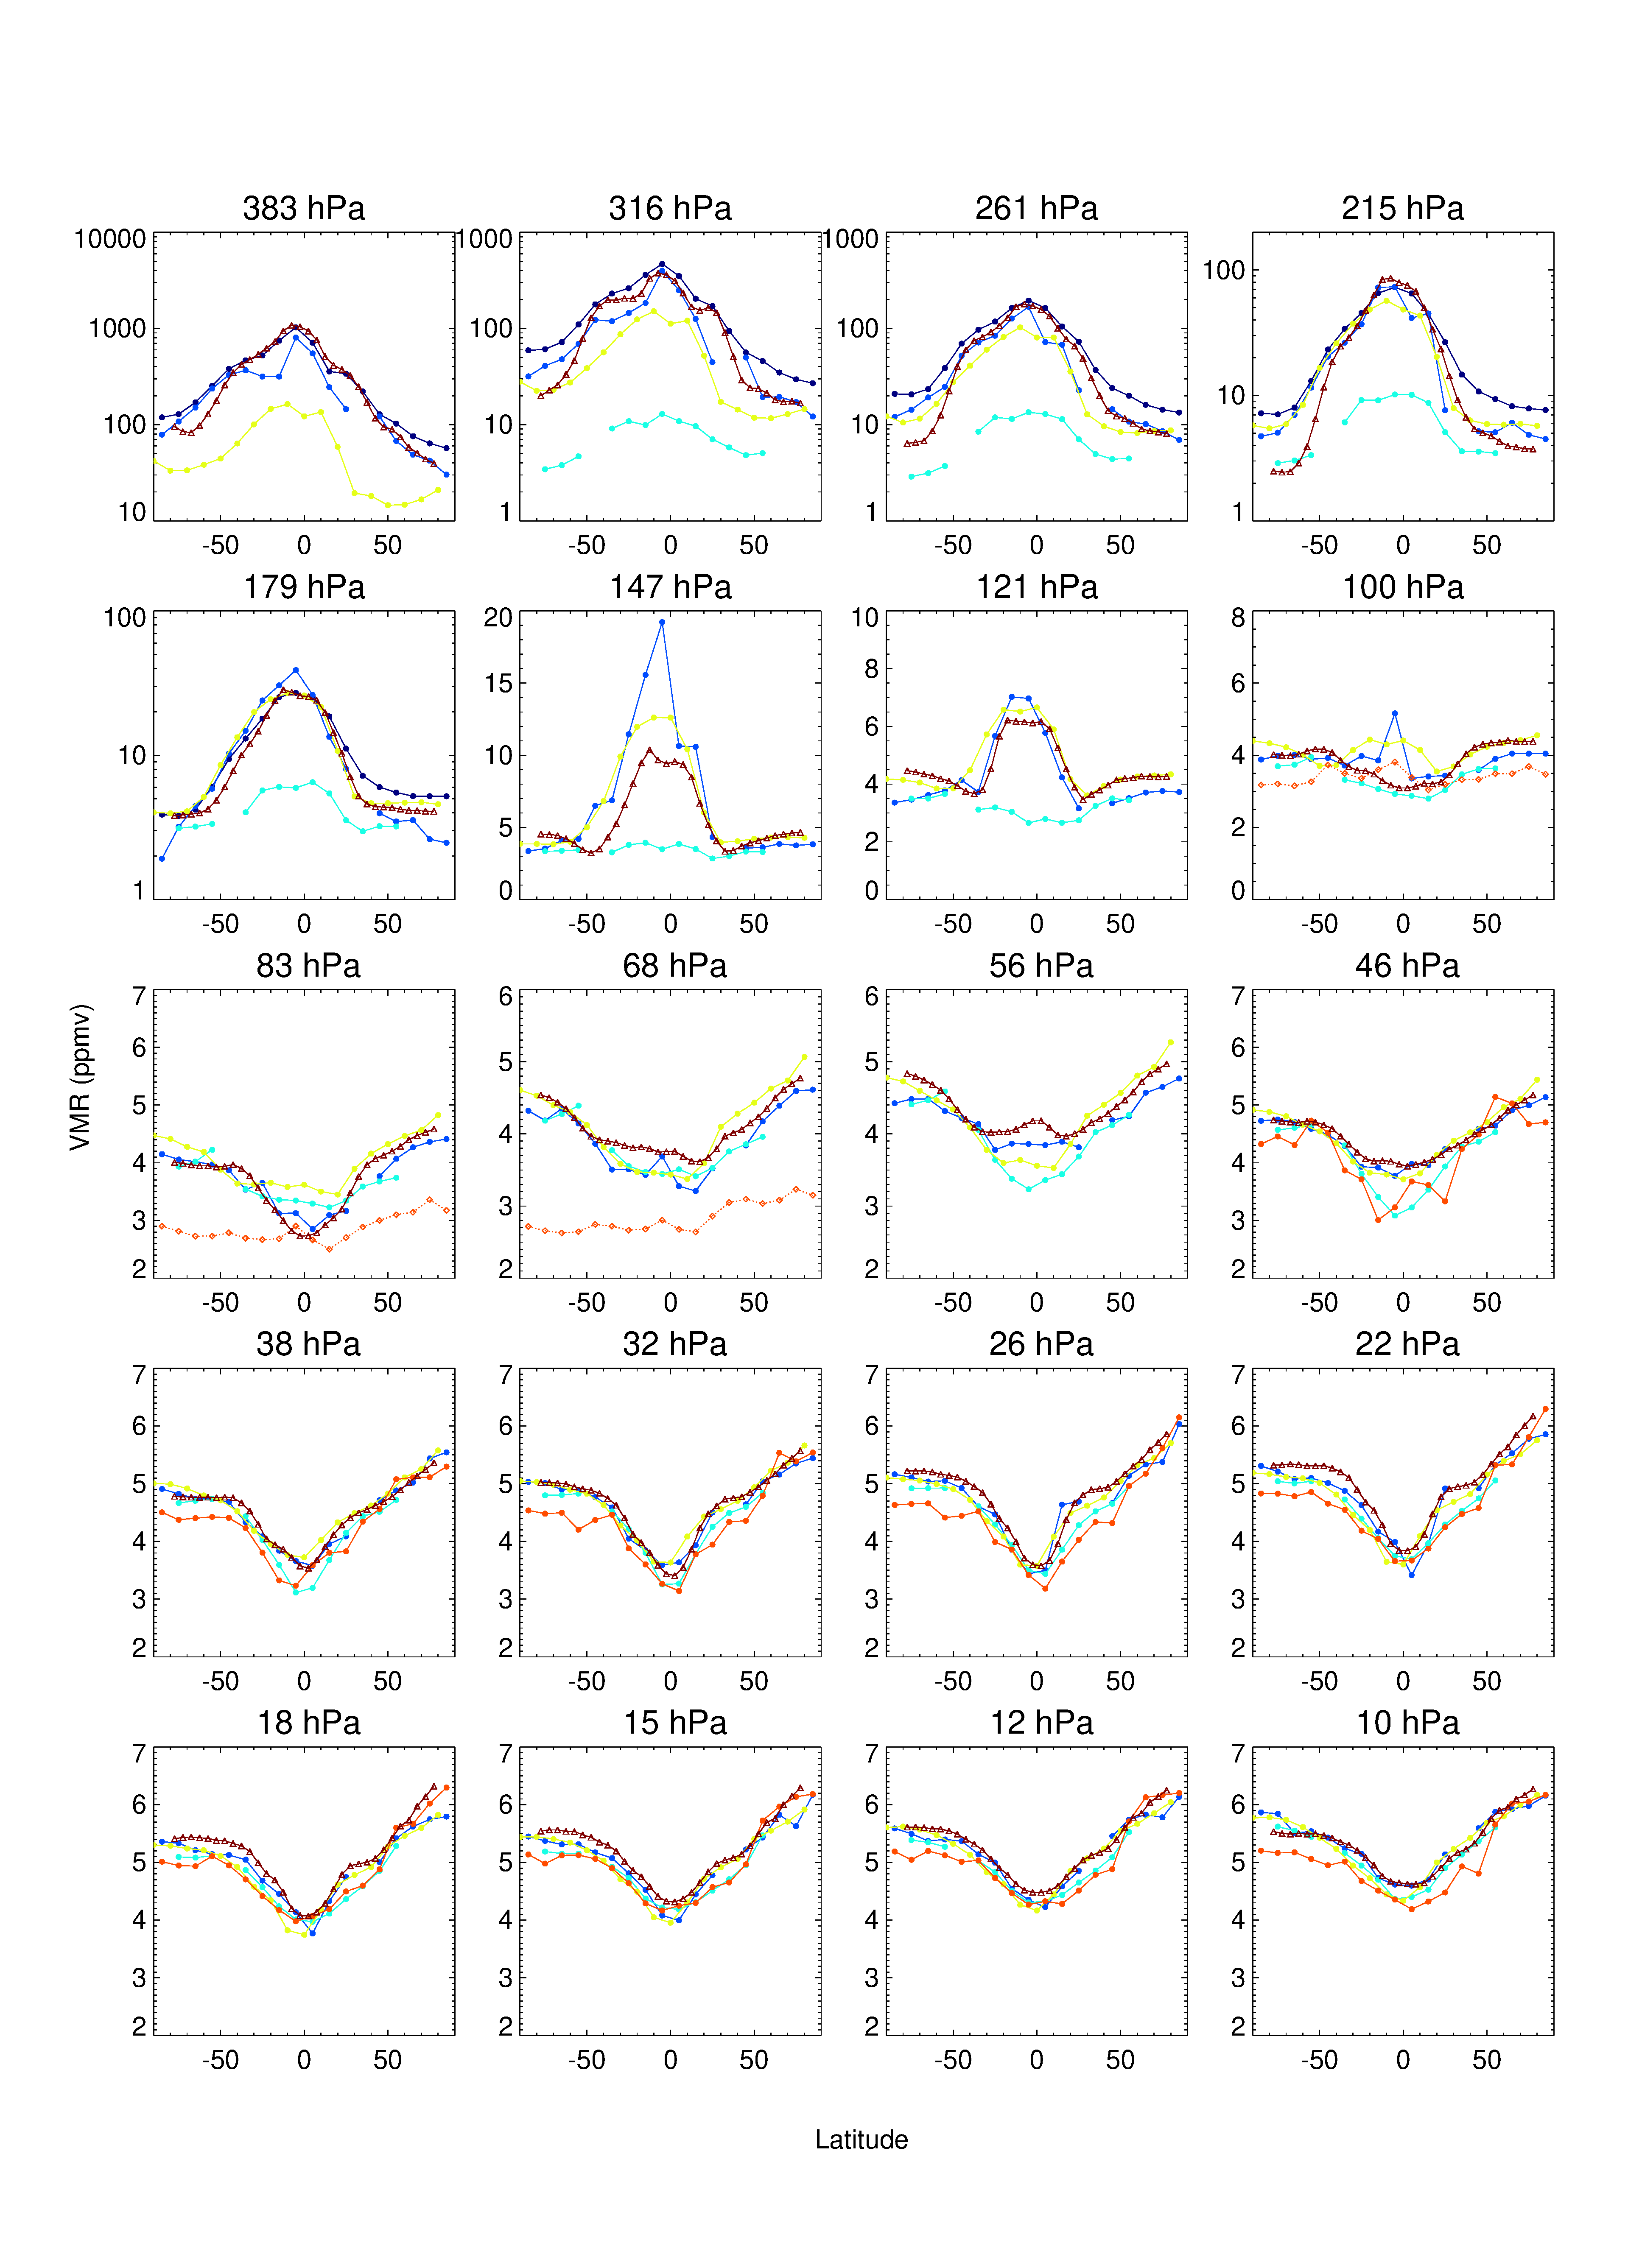
\includegraphics[bb = 58 120 1776 2340, clip, width=0.9\linewidth]{figures/sat_h2o_comps}
\end{center}
\caption{A comparison of MLS \thisv (red) water vapor for Jan-Feb-Mar
  2009 with other satellite observations shown as latitude-value zonal
  means. Each panel represents a pressure surface. The satellites are:
  AIRS v6 (dark blue), ACE-FTS v3.5 (light blue), MIPAS IMK v4
  (yellow-green), HALOE v19 (cyan), Odin SMR 544 GHz continuum product
  (orange open diamonds), and Odin SMR line resolved product (orange
  solid bullets).}
\label{fig:satcomps}
\end{figure}

Figure~\ref{fig:satcomps} shows a latitude-value zonal mean comparison
among several satellite data sets. The satellite datasets include MLS
\thisv, AIRS v6, ACE-FTS v3.5, MIPAS IMK v4, HALOE v19, Odin SMR
continuum H\cs2O, and Odin SMR line resolved H\cs2O. The data sets
show agreement for the stratospheric levels shown here beginning with
32~hPa and lower. More significant departures exist amongst them between
121--38~hPa even showing different latitude stucture. Averaging kernels
were not applied here because the nominal resolution of these datasets are
similar but each data set will exhibit its own vertical smoothing and
\emph{a priori} dependencies which is a contributing factor to the
differences where a sharp vertical gradient change at the tropopause occurs.
The patterns are more similar for the upper tropospheric levels (316--147~hPa).

One potential improvement in \thisv is shown in
Figures~\ref{fig:airsmlsjfm2009maps} and \ref{fig:airsmlsjja2009maps}
that compare multi-month maps of MLS with AIRS v6. The very moist
regions over the tropics in \prevv and \thisv are drier than in v2.2 and v3.3
for the higher pressure levels and in better agreement with AIRS.

\begin{figure}
\begin{center}
  \includegraphics[width=0.9\linewidth]
{figures/grid_maps_jfm2009_airsv6-mlsv2-3-4-5.png}
\end{center}
\caption{Mapped fields from AIRS v6 (left), MLS v2.2 (center-left), MLS
  v3.3 (center), MLS \prevv (center-right), and MLS \thisv (right) pressures
  between 300\,--150\,hPa for Jan-Feb-Mar 2009. The black-white lines indicate
  the tropopause where the region poleward is in the stratosphere.
  Note that the AIRS measurement is mostly suitable for H\cs2O greater than
  10\,ppmv.}
\label{fig:airsmlsjfm2009maps}
\end{figure}

\begin{figure}
\begin{center}
  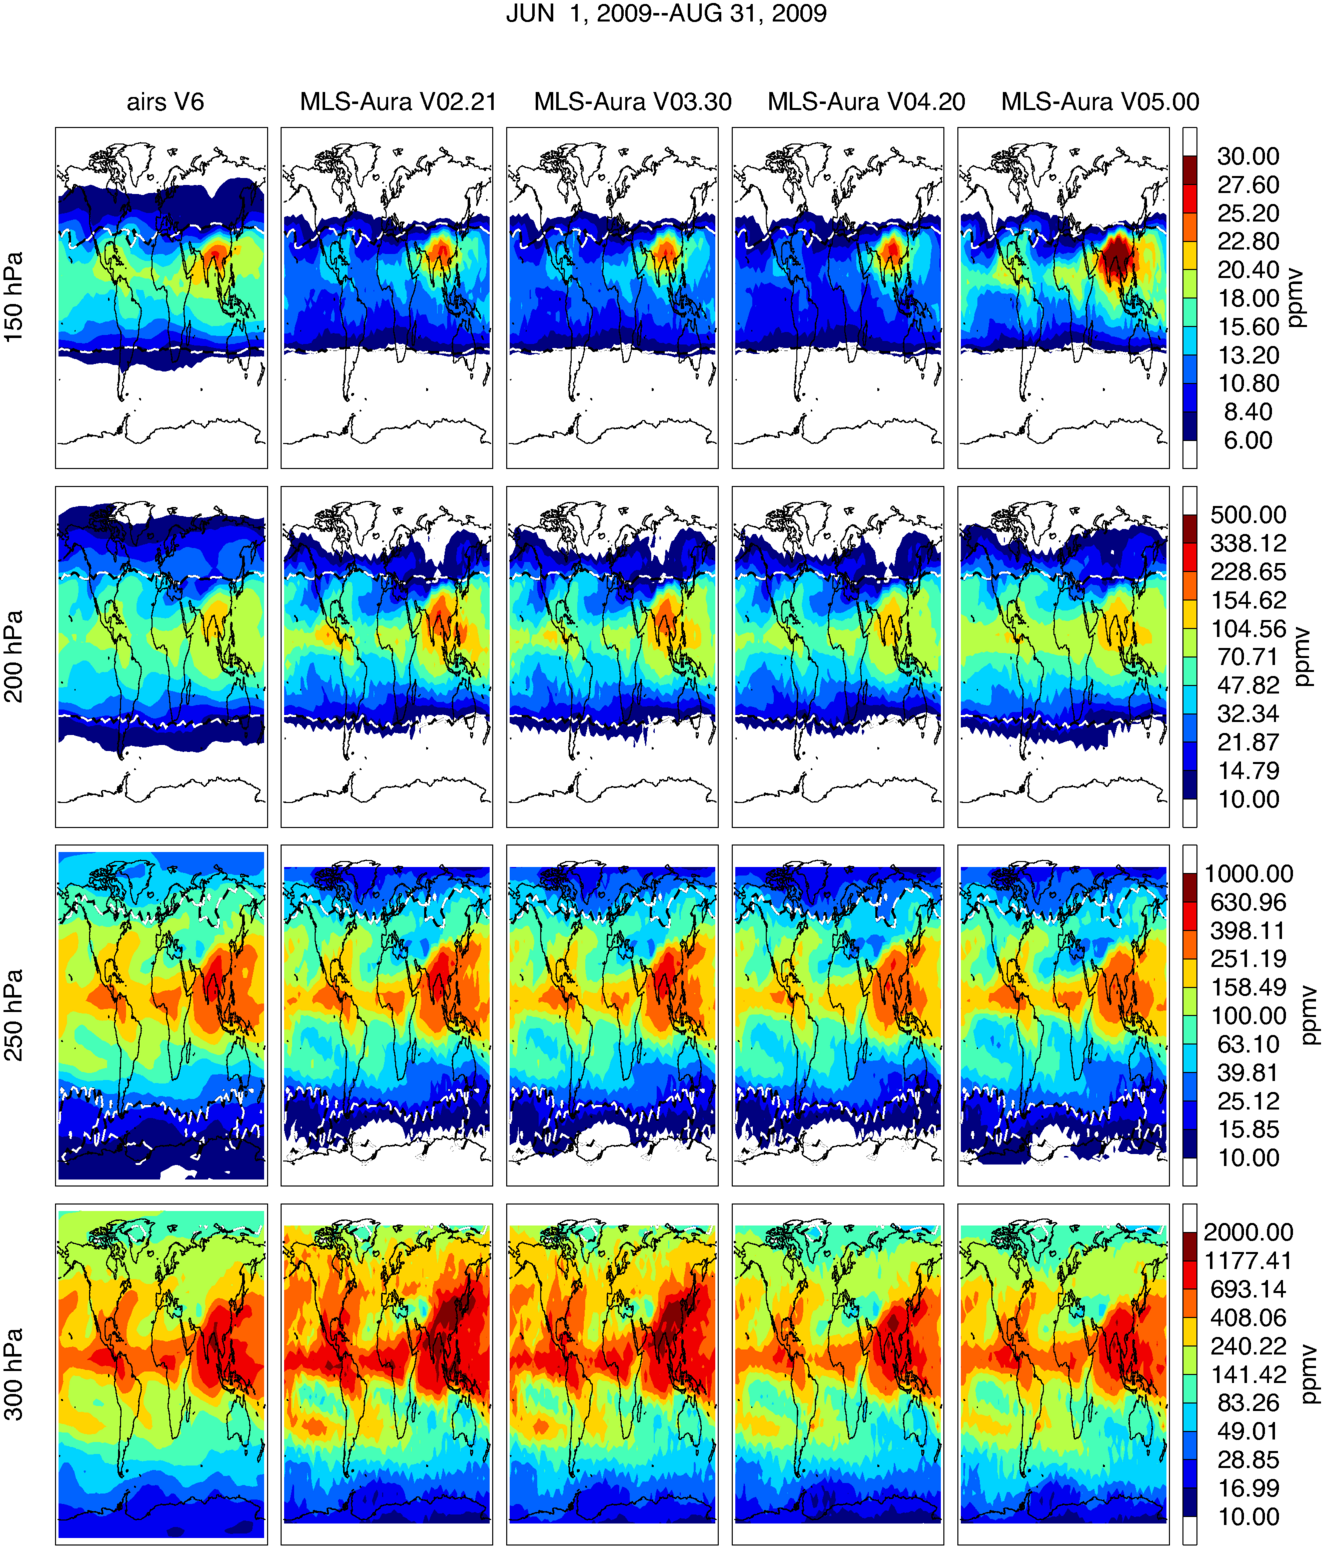
\includegraphics[width=0.9\linewidth]
{figures/grid_maps_jja2009_airsv6-mlsv2-3-4-5.png}
\end{center}
\caption{Mapped fields from AIRS v6 (left), MLS v2.2 (center-left), MLS
  v3.3 (center), MLS \prevv (center-right), and MLS \thisv (right) pressures
  between 300\,--\,150 hPa for Jun-Jul-Aug 2009. The black-white lines indicate
  the tropopause where the region poleward is in the stratosphere. 
  Note that the AIRS measurement is mostly suitable for H\cs2O greater than
  10\,ppmv.}
\label{fig:airsmlsjja2009maps}
\end{figure}

Apart from the differences noted above, the MLS \thisv H\cs2O is similar
to \prevv, v3.3, and v2.2 products, the latter described and
validated in \citet{ReadEtal:2007} and \citet{LambertEtal:2007}. The H\cs2O
validation paper used AIRS v4 and MLS v2 humidities and both of them
have become more dry in their subsequent versions. A revised validation
paper for H\cs2O is not planned in the near future and users are
encouraged to read \citet{ReadEtal:2007} and \citet{LambertEtal:2007} for more
information. MLS v4.2 is a part of the second SPARC Water Vapor
Assessment (WAVAS-II) activity.

\subsection{Potential drift in lower stratospheric water vapor}
\label{sec:H2ODrift}

Comparisons of lower stratospheric H\cs2O between MLS and balloon-borne CFH
and FPH\footnote{Cryogenic Frostpoint Hygrometer (CFH) and Frost Point
Hygrometer (FPH)} from 2004 to the present time show a drift in the agreement
with MLS water vapor increasing at a rate of
\mbox{0.03\,--\,0.07\,ppmv\,yr\cp{-1}} relative to the frostpoint sondes
(roughly 0.6 to 1.5\% per year), starting around 2009 \citet{HurstEtal:2016}.
Comparisons with the ACE-FTS instrument, and with measurements of upper
stratospheric water vapor from ground-based microwave sensors, provide
evidence for a smaller (\texttildelow+0.2\% per year) drift. The new
calibration values for the sideband fraction that are updated monthly are
yet smaller but approaching the drift seen with ACE-FTS but will significantly
underestimate the larger drift reported by \citeauthor{HurstEtal:2016}. A
complete assessment of the drift correction will have to wait until more
reprocessed data becomes available.

\subsection{Data screening}
\label{sec:H2OScreening}
\begin{description}
\item[Pressure range:] \screeningrule{316\,--\,0.00046\,hPa.}
  \standardrangestatement\,Using data at 0.00046\,hPa requires consultation
  with the MLS team.
\standardprecisionrule
\evenstatusrule
\item[Clouds:] Ignore status bit 16 (high cloud) or bit 32 (low cloud) set
indicating the presence of clouds. See artifacts for more details.
\item[Quality field:] \screeningrule{Only profiles with a value of the
    \texttt{Quality} \emph{greater} than 0.7 should be used in
    scientific studies.}  The quality threshold is deliberately set low
    because it is not a very good discriminator of poor profiles except when
    quality is well below the mean value; therefore,
    we recommend the ``additional screening to avoid outliers,'' as described
    below.
\item[Convergence field:] \screeningrule{Only profiles with a value of
    the \texttt{Convergence} \emph{less} than 2.0 should be used in
    scientific studies.}
\item[Additional screening to avoid outliers:] After application of
  the \texttt{Status}, \texttt{Quality}, and \texttt{Convergence}
  screening described above, there remain some unphysical profiles in
  the MLS \thisv\ H\cs2O dataset. These are characterized by
  unrealistically low water vapor mixing ratios in the upper troposphere
  and stratosphere. The cause behind this behavior is from using the
  logarithmic basis which excludes negative values. Sometimes the retreival
  minimizer seeks a negative value (at a given level and is almost always 
  accompanied with severe vertical profile oscillations) which is not
  allowed and therefore an optimal fit to the measurement signal is
  not achieved. H\cs2O profiles having values less than 0.101~ppmv
  (0.101$\times 10^{-6}$VMR) at any pressure at or higher than 1\,hPa
  (vertical levels 1--37) should not be used. Profiles with acceptable
  \texttt{status}, \texttt{quality}, and \texttt{convergence} with values
  less than 0.101~ppmv at pressures $<$ 1~hPa (vertical levels 38--55) are
  acceptable and occur frequently because the water vapor
  concentration in the mesosphere is often less than the measurement
  precision and negative values are preferable but not allowed due to the
  logarithmic basis definition being used.
 
\end{description}

\subsection{Artifacts}

There is a minimum concentration where MLS H\cs2O measurements become
unreliable. This is given in Table~\ref{tab:H2OSummary} under the ``Min.
H\cs2O'' column. The lowest allowable H\cs2O value is 0.1\,ppmv.
Differences between the retrieved middle tropospheric H\cs2O constraint
and the true atmospheric state can cause errors at 316 and 261\,hPa.
The error manifests either as dry ($<$1\,ppmv) or moist spikes in an
orbital time series. Such data are often accompanied with good quality
and status but is rejected by checking the profile for such events.

Clouds in the field of view degrade the data in unpredictable ways. Many
instances of quality $<$0.7 occur in the presence of clouds where the
cloud screening of the radiances failed to reject them. Cloud radiative
scattering distorts the spectral lineshape causing poor fits and low
quality values.  However, not all MLS signals are obviously
affected. Coincident comparisons of MLS cloud flagged H\cs2O
(\texttt{status} bit 16 or 32 set between 316\,--\,215\,hPa) having good
quality with AIRS show a small mean bias of 10\% but exhibit a 50\% increase
in variability for the individual differences. Therefore users should be
aware that, although the overall biases for measurements inside clouds
are similar to that for clear sky, individual profiles will exhibit
greater variability about the true atmospheric humidity.

The 190~GHz radiometer signals due to aging are drifting. This drift manifests
as a change in the sideband fraction. \thisv makes an attempt to correct this.

In the mesosphere, the precision is often larger than the
retrieved value and therefore negative concentrations are possible and
proper. The logarithmic definition of the H\cs2O basis doesn't allow retrieval
of negative values with the minimum lowest allowed concentration being 0.1~ppmv.
Therefore an average of many profiles will produce a positive bias. It is
recommended that a better representation of the average of many profiles is
achieved by calculating its median.

The instrument scan nomimnally tops out at 0.001~hPa. Therefore,
the 0.00046~hPa which is now retrieved in \thisv is not a vertically
resolved measurement but rather a column amount from 0.001~hPa to the
spacecraft under the constraint that all levels above 0.00046~hPa are fixed
at \emph{a priori} values. What this means is that should there be a large
H\cs2O event in any level above 0.00046~hPa would be retrieved as an
enhanced event at 0.00046~hPa but its vertical location above 0.00046~hPa is
unknown.

\subsection{Desired improvements for future data version(s)}

While many defects in v4.2 and earlier versions have been addressed,
futher investigation to their effectiveness, especially the drift
reduction and high latitude low value retrievals in the upper
troposphere needs to be assessed and improved upon if necessary.
Possibly a vertically resolved H\cs2O product for
pressure $>316\,\text{hPa}$ at high latitudes during dry conditions.

\begin{table}
\caption{Summary of MLS \thisv H\cs2O product.}
\vspace{\tablecaptionsep}
\label{tab:H2OSummary}
\begin{minipage}{\linewidth}
\centering\begin{tabular}{cccccm{30ex}}
\toprule
\parbox{10ex}{\centering\bfseries Pressure / hPa} &
\parbox{11ex}{\centering\bfseries Resolution V$\times$H / km} &
\parbox{10ex}{\centering\bfseries Precision\footnote{Precision for a
    single MLS profile} / \%} &
\parbox{10ex}{\centering\bfseries Accuracy / \%} &
\parbox{10ex}{\centering\bfseries Min. / ppmv\footnote{Minimum H\cs2O is an estimate of the minimum H\cs2O 
concentration measurable by \thisv MLS.}} &
\parbox{11ex}{\centering\bfseries Comments} \\
\midrule
$\le$0.00022  & --- & --- & --- & --- & Unsuitable for scientific use \\
0.0005 & NVR\footnote{Not Vertically resolved (NVR)}  $\times$ TBD & 900 &
TBD\footnote{Not yet determined} & 0.1 & Nominally a slant column measurement
for p $\le$ 0.001 hPa. \\
0.001 & TBD  $\times$ TBD &450 & TBD\footnote{Not yet determined} & 0.1 & \\
0.002 & 10.3 $\times$ 350 &152 & 40 & 0.1 & \\
0.005 & 10.8 $\times$ 585 & 81 & 23 & 0.1 & \\
0.010 &  8.8 $\times$ 725 & 55 & 17 & 0.1 & \\
0.022 &  8.0 $\times$ 745 & 41 & 19 & 0.1 & \\
0.046 &  7.4 $\times$ 540 & 35 & 17 & 0.1 & \\
0.10 &  5.8 $\times$ 745 & 24  & 14 & 0.1 & \\
0.22 &  3.6 $\times$ 670 & 19  & 11 & 0.1 & \\
0.46 &  3.3 $\times$ 505 & 12  &  8 & 0.1 & \\
1.0 &  2.5 $\times$ 400 &  6   &  7 & 0.1 & \\
2.2 &  3.5 $\times$ 385 &  4   &  7 & 0.1 & \\
4.6 &  3.4 $\times$ 350 &  4   &  5 & 0.1 & \\
10 &  2.8 $\times$ 290 &  6    & 19 & 0.1 & \\
22 &  3.2 $\times$ 265 &  5    &  5 & 0.1 & \\
46 &  3.2 $\times$ 230 &  5    &  4 & 0.1 & \\
68 &  3.1 $\times$ 190 &  5    &  9 & 0.1 & \\
83 &  3.1 $\times$ 190 &  7    &  9 & 0.1 & \\
100 & 3.0 $\times$ 198 & 15 &  8 & 0.1 & \\
121 & 2.6 $\times$ 193 & 20 & 12 & 0.1 & \\
147 & 2.3 $\times$ 188 & 20 & 15 & 0.1 & \\
178 & 1.7 $\times$ 183 & 25 & 20 & 3  & \\
\addlinespace
215 & 1.6 $\times$ 178 & 40  & 25 & 3   & Extent of a low bias for latitudes
$>60\degsym$ to be investigated. \\
\addlinespace
261 & 1.4 $\times$ 173 & 35  & 20 & 4   & Extent of low bias for latitudes
$>60\degsym$ to be invesrtigated. \\
\addlinespace
316 & 1.3 $\times$ 168 & 65  & 15 & 7   & Occasionally erroneous low value
$<1\,\text{ppmv}$ and high value fliers are retrieved in the tropics, usually in
clouds. \\
\addlinespace
$>316$ & --- & --- & --- & --- & Unsuitable for scientific use \\
\bottomrule
\end{tabular}
\end{minipage}
\end{table}


%%% Local Variables: 
%%% mode: latex
%%% TeX-master: "v5-x-report"
%%% End: 

\speciestitle{Hydrogen Chloride}{HCl}{HCl}{%
\item[Useful range:] 100\,--\,0.32\,hPa 
\item[Contact:] Lucien Froidevaux,
  \email{Lucien.Froidevaux@jpl.nasa.gov}}
\label{sec:standardHCl}

\subsection*{Introduction}

As in the previous MLS HCl data version, v2.2, the MLS \thisv retrievals
of the HCl standard product (from the 640\,GHz radiometer) use channels
from band 14, as a result of the deterioration observed since early 2006
in nearby band 13, originally targeted (with narrower channels than band
14) at the main HCl emission line center.  Full measurement days with
band 13 on from February 15, 2006, to the time of writing (May 2013) are
as follows: March~15, 2006 (2006d074), April~14, 2006 (2006d104),
January~6 through~8, 2009 (2009d006\,--\,2009d008), and January~24
through~27, 2010 (2010d024\,--\,2010d027). For days prior to February
16, 2006 and for the few days (as listed above) when band 13 is turned
on thereafter, the MLS Level~2 software also produces a separate
\texttt{HCl-640-B13} product (stored in the \texttt{L2GP-DGG} file),
using the band 13 radiances.  This product has slightly better precision
and vertical resolution in the upper stratosphere than the standard HCl
product.  The MLS team plans to turn band 13 on for a few days about
once every year or two (or maybe even less frequently) in order to
preserve its lifetime, estimated at a few days to a few weeks, based on
the channel counts and channel noise characteristics observed during the
3-day turn-on period in late January, 2010.  It is possible/likely that
this band will not be turned on again for a number of years.  Band 13
should provide better trend information for upper stratospheric data,
given its narrower channels.  Upper stratospheric trends from the
(uninterrupted 2004 to present) band 14 retrievals are too small,
compared to band 13 data and expectations (as well as versus ACE-FTS HCl
data).

\begin{figure}
  \centering\dontincludegraphics[angle=90,width=\linewidth]%
  {figures/HCl_2bands_0p46hpa_trends_2004_2010}
  \caption{Daily zonal averages for MLS HCl at 0.46\,hPa, from
    mid-August, 2004, through January, 2010, for the originally-targeted
    band 13 measurements (red points), now available only on occasion
    (to preserve lifetime), and the band 14 data (blue points).  The
    lines are simple linear fits through the daily data points; trend
    differences are apparent in this region of the atmosphere, where the
    information obtained from band 14 HCl data is not reliable enough.}
\label{fig:MLSHCl2bands}
\end{figure}


See Figure~\ref{fig:MLSHCl2bands} for an illustration of the trend
differences between these two MLS band measurements of upper
stratospheric HCl.  In the lower stratosphere, however, variations in
the two HCl products are closer together, and seasonal/geographical
variability are more pronounced.  We believe that the band 14 daily
global retrievals are completely suitable for use in studies of seasonal
and geographical variations (e.g., during polar winter/spring).

Table~\ref{tab:HClSummary} summarizes the MLS HCl resolution, precision,
and accuracy estimates as a function of pressure.  More discussion and
data screening recommendations for the MLS HCl \thisv data are provided
below.  Analyses describing detailed validation of the MLS (v2.2)
product and comparisons with other data sets are described in
\citet{FroidevauxEtal08HCl}.  Based on the fairly small overall changes
in \thisv HCl data (versus v2.2), the conclusions of the latter reference
should remain essentially unchanged.  Any minor updates will result from
new comparisons between MLS (\thisv) HCl and ACE-FTS HCl, which is also
being updated to a newer version (version 3).  We do not expect the
systematic uncertainty estimates in Table~\ref{tab:HClSummary} to change
significantly; however, an MLS team review of those estimates is
anticipated.

\subsection*{Changes from  v2.2}

While there were no large \thisv algorithmic changes relating to HCl, one
difference in the retrievals for HCl and other products derived from the
640-GHz MLS retrievals is that temperature information is now obtained
from the first retrieval phase (`Core'), as opposed to the 640-GHz
phases themselves; this led to overall improved efficiency, convergence,
and stability for the \thisv 640-GHz products.  A Level~1 change,
resulting from a small error in the spectral calibration files, which
led to all filter channel responses being shifted by a small fraction
(1$\%$) of the nominal channel widths, also had an impact on the HCl
results.  Mainly because of this change, \thisv MLS HCl abundances near
and just above the stratopause are a few percent less than the v2.2
abundances, and exhibit a steeper slope near very the top of the
recommended pressure range.  The slight oscillating behavior in HCl near
0.15 to 0.1\,hPa has led us to change the top boundary for recommended
HCl profiles to the MLS retrieval level at 0.32\,hPa.  This issue does
not seem to affect the band 13 MLS measurement of HCl, which can in
principle be used (on available measurement days) up to the 0.15\,hPa
level.

Other changes relating to the treatment of forward model radiance
continuum had an impact on species in the 640-GHz retrievals (mainly in
the lower stratosphere).  The background observed in the 640 GHz
radiances includes emissions from N\cs2, O\cs2, and H\cs2O.  There are
laboratory-based and ground-based models for the continuum absorptions
that are the basis for the MLS absorption model [{\it Pardo, 2001}, and
references therein].  These models were tested against MLS extinction
measurements from the wing channels in the 640 GHz radiometer; the
latitude dependence of this extinction was found to agree better with
the expected most plus dry continuum extinction values if the dry and
moist continuum functions were scaled by factors close to 20\%.  The
incorporation of this change improved the lower stratospheric retrievals
of most of the 640-GHz species (generally in terms of average negative
biases and their latitude dependence).

A comparison plot showing zonal average HCl contours and differences
between the two data versions for a typical month (April, 2006) is
provided in Figure~\ref{fig:MLSv2v3HClContour}.  For pressures larger
than or equal to 0.22\,hPa, the average differences between the two data
versions are typically within 0.1\,ppbv (a few percent).  The average
changes (globally within a few percent in most of this pressure range
for typical months) are within the estimated accuracy values (see
Table~\ref{tab:HClSummary}), which we have now changed (increased) to a
value of 10$\%$ (or about 0.3 ppbv) for pressures less than 10\,hPa,
given the trend issue for upper stratospheric HCl mentioned above.  The
largest percentage changes in HCl occur for very small mixing ratio
values; \thisv values can be larger than the v2.2 values by 20 to 50$\%$
(or more) under low HCl conditions in the lower stratosphere at low
latitudes or during winter at polar latitudes, even if these percentages
typically only reflect an increase of 0.1 ppbv (or less).  On occasion,
however, v2.2 zonal averages at 100\,hPa (mainly) or during southern 
hemisphere polar winter conditions at low altitude were slightly negative; 
this is no longer the case for \thisv data.  Whether the larger \thisv values 
at 100\,hPa (with averages now slightly above 0.1\,ppbv at low latitudes) 
are more realistic than v2.2 data remains to be seen, but this is a fairly 
minor change.  The precision estimated in the Level~2 files is essentially
unchanged from v2.2.

\begin{figure}
  \centering\dontincludegraphics[angle=90,width=\linewidth]{figures/HCl_v2_v3_Contour_2006m04}
\caption{Zonal averages for MLS HCl profiles during April, 2006, showing
  the MLS v2.2 HCl mixing ratio contours (top left panel), the \thisv
  contours (top right panel), and their differences in ppbv (\thisv minus
  v2.2, bottom left panel) and percent (\thisv minus v2.2 versus v2.2,
  bottom right panel).}
\label{fig:MLSv2v3HClContour}
\end{figure}

%\begin{figure}
%\centering\dontincludegraphics[angle=90,width=1.\linewidth]{figures/HCl...}
%\caption{Zonal average profiles ...}
%\label{fig:avk-HCl}
%\end{figure}

\subsection*{Resolution}
\onestandardavk{HCl}{HCl}%

Typical (rounded off) values for resolution are provided in
Table~\ref{tab:HClSummary}.  Based on the width of the averaging kernels
shown in Figure~\ref{fig:AvkHCl}, the vertical resolution for the
standard HCl stratospheric product is \texttildelow3\,km (2.7\,km at best in
the lower stratosphere), or about double the 640\,GHz radiometer
vertical field of view width at half-maximum; the vertical resolution
degrades to 4--6\, km in the lower mesosphere.  The along-track
resolution is \texttildelow200 to 350\,km for pressures of 2\,hPa or more, and
\texttildelow500\,km in the lower mesosphere.  The cross-track resolution is
set by the 3\,km width of the MLS 640\,GHz field of view.  The
longitudinal separation of MLS measurements, set by the Aura orbit, is
10\degsym\,--\,20\degsym\ over middle and lower latitudes, with much
finer sampling in polar regions.

\subsection*{Precision}

The estimated single-profile precision reported by the Level~2 software
varies from \texttildelow0.2 to 0.6\,ppbv in the stratosphere (see
Table~\ref{tab:HClSummary}), with poorer precision obtained in the lower
mesosphere.  These precision values have not changed significantly for
\thisv data.  The Level~2 precision values are often only slightly lower
than the observed scatter in the data, as evaluated from a narrow
latitude band centered around the equator where atmospheric variability
is often smaller than elsewhere, or as obtained from a comparison
between ascending and descending coincident MLS profiles.  The scatter
in MLS data and in simulated MLS retrievals (using noise-free radiances)
becomes smaller than the theoretical precision (given in the Level~2
files) in the upper stratosphere and mesosphere, where there is a larger
impact of a priori and smoothing constraints.  The HCl precision values
increase rapidly at pressures less than 0.2\,hPa, and are generally
flagged negative at pressures less than 0.1\,hPa; this indicates an
increasing influence from the \emph{a priori} (with poorer measurement
sensitivity and reliability).

\subsection*{Accuracy}

The accuracy estimates in the Table for v2.2 data came from a
quantification of the combined effects of possible systematic errors in
MLS calibration, spectroscopy, etc.\ on the HCl retrievals.  These
values are intended to represent 2 sigma estimates of accuracy.  For
more details, see the MLS validation paper by
\citet{FroidevauxEtal08HCl}.  For \thisv, however, given the trend issues
affecting the (band 14) standard HCl product in the upper stratosphere
and lower mesosphere, we now need to recommend a more conservative
accuracy estimate of 10\% in this region (or about 0.3 ppbv), rather
than the smaller numbers from the original (formal) estimates, which
should still apply to the (now very occasional) band 13 retrievals.
Given the better agreement between the two bands' retrievals in the
lower stratosphere, we maintain the formal accuracy estimates in this
region (see Table~\ref{tab:HClSummary}). Data users should be able to
reliably study seasonal and geographical changes in lower stratospheric
HCl (e.g., at high latitudes in winter or spring) with the current (band
14) standard HCl product.

\subsection*{Data screening}
\begin{description}
\item[Pressure range:] \screeningrule{100\,--\,0.32\,hPa}
  \standardrangestatement\ We note that the MLS values at 147\,hPa are
  are biased high, at least at low to mid-latitudes, and slightly more
  in the \thisv data than in the v2.2 data -- and these values are not
  recommended (particularly at low latitudes). Also, although the
  vertical range at the top end is recommended up to 0.32\,hPa, users
  should note the significant issues relating to HCl trend estimates in
  the upper stratosphere and lower mesosphere; average profiles in this
  region can be used for studies not involving trends (or accuracy
  requirements not as tight as 10\%).  The use of the band 13
  (intermittent) HCl data can/will continue to be carefully evaluated
  for trend-related issues.  
\standardprecisionrule \evenstatusrule

\item[Clouds:] \cloudsokrule

\item[Quality:] \qualityrule{1.2} This criterion removes profiles
  with the poorest radiance fits, typically significantly less than
  1$\%$ of the daily profiles. Results in this respect have improved, in
  comparison to v2.2 data.  For HCl (and for other 640\,GHz MLS
  products), this screening correlates well with the poorly converged
  sets of profiles (see below); we recommend the use of both the
  \texttt{Quality} and \texttt{Convergence} fields for data screening.
  The use of this screening criterion sometimes (but rarely) removes up
  to a few percent of global daily data (for example, during the first
  half of September, 2006, when some high latitude convergence and
  quality issues arose).

\item[Convergence:] \convergencerule{1.05} For the vast majority
  of profiles (99\% or more for most days), this field is less than
  1.05.  Results in this respect have improved, in comparison to v2.2
  data.  Nevertheless, on occasion, sets of profiles (typically one or
  more groups of ten profiles, retrieved as a `chunk') have this
  \texttt{Convergence} field set to larger values.  These profiles are
  usually almost noise-free and close to the \emph{a priori} profile,
  and need to be discarded as non-converged.  The \texttt{Quality} field
  (see above) most often yields poorer quality values for these
  non-converged profiles. The use of this screening criterion sometimes
  (but rarely) removes up to a few percent of global daily data (for
  example, during the first half of September, 2006, when some high
  latitude convergence and quality issues arose).
\end{description}

\subsection*{Review of comparisons with other datasets}

\citet{FroidevauxEtal08HCl} provided results of generally good comparisons
between MLS HCl and other satellite, balloon, and aircraft measurements.
Both MLS and ACE-FTS HCl values are generally larger (by about 10 to 15\%) 
than the HCl values from HALOE, especially at upper stratospheric altitudes; 
this feature has not changed, overall, with the new data version(s) from 
both MLS and ACE-FTS.  MLS HCl at 147\,hPa is biased high versus WB-57 aircraft 
in-situ (CIMS) measurements (low to mid-latitudes); while this is still true 
for \thisv data, MLS data on this pressure level may be useful and accurate enough 
at high latitudes. 

\subsection*{Artifacts}
\begin{itemize} 
\item We do not recommend the use of the MLS HCl standard product (from
  band 14) in the upper stratosphere and lower mesosphere, in terms of
  detailed trend studies, for reasons mentioned above.  The MLS HCl
  global results from band 13, although very infrequent (after early
  2006), are observed (and expected) to be more reliable in this
  respect.
\item The HCl values at 147\,hPa are biased high and generally not
  usable (except possibly at high latitudes).  Please consult the MLS
  team for further information.
\item Users should screen out the non-converged and poorest quality HCl
  profiles, as such profiles (typically a very small number per day)
  tend to behave unlike the majority of the other MLS retrievals.  See
  the criteria listed above.
\end{itemize}  

\begin{table}
\caption{Summary for MLS hydrogen chloride}
\vspace{\tablecaptionsep}
\label{tab:HClSummary}
\begin{minipage}{\linewidth}
\centering\begin{tabular}{ccccccm{25ex}}
\toprule
\parbox[m]{15mm}{\centering\textbf{Pressure}} &
\multicolumn{2}{c}{\parbox[m]{15mm}{\centering\textbf{Precision
      \footnote{Precision (1 sigma) for individual profiles; note that
        $\%$ values tend to vary strongly with latitude in the
        lower stratosphere.}}}} &
\parbox[m]{24mm}{\centering\textbf{Resolution\\ V $\times$ H}} &
\multicolumn{2}{c}{\parbox[m]{15mm}{\centering\textbf{Accuracy%
      \footnote{2 sigma estimate from systematic uncertainty
        characterization tests (but see text for estimates at 
        pressures lower than 10\,hPa); note that percent values tend 
        to vary strongly with latitude and season in the lower 
        stratosphere, due to the variability in HCl.}\\}}} 
&
\textbf{Comments} \\
\textbf{hPa} & \textbf{ppbv} & \textbf{\%} & \textbf{km} & \textbf{ppbv} & \textbf{\%} & \\
\midrule
0.2            & --- & ---             & ---              & ---   & ---     & Unsuitable for scientific use \\  
0.5            & 0.7 &   20            &   5 $\times$ 400 & 0.3   &   10    & Unsuitable for trend studies \\
1              & 0.5 &   15            &   4 $\times$ 300 & 0.3   &   10     & Unsuitable for trend studies \\
2              & 0.4 &   15            &   3 $\times$ 250 & 0.3   &   10     & Unsuitable for trend studies \\
5              & 0.3 &   10            &   3 $\times$ 200 & 0.3   &  10     & Unsuitable for trend studies \\
10             & 0.2 &   10            &   3 $\times$ 200 & 0.2   &  10     & \\
20             & 0.2 &   15            &   3 $\times$ 200 & 0.1   &  10     & \\
46             & 0.2 & 10 to $>$ 40    &   3 $\times$ 250 & 0.2   &  10 to $>$ 40  & \\
68             & 0.2 & 15 to $>$ 80    &   3 $\times$ 300 & 0.2   &  10 to $>$ 80   &  \\
100            & 0.3 & 30 to $>$ 100   &   3 $\times$ 350 & 0.15  &  10 to $>$ 100  &  \\
147            & 0.4 & 50 to $>$ 100   &   3 $\times$ 400 & 0.3  &   50
to $>$ 100  & High bias at low lats. (use with caution elsewhere) \\  
\bottomrule
\end{tabular}
\end{minipage} 
\end{table}

%%% Local Variables: 
%%% mode: latex
%%% TeX-master: "v4-x-report"
%%% End: 

\speciestitle{Hydrogen Cyanide}{HCN}{HCN}{%
  \item[Useful range:] 68--32\,hPa (use with caution) 21--0.1\,hPa (no restrictions)
  \item[Product lead:] Hugh C. Pumphrey
  \item[Contact:] Luis Mill\'an,
 \email{Luis.F.Millan@jpl.nasa.gov}}

\subsection{Introduction}

MLS observes \ch{HCN} emission lines within the 190-GHz radiometer. The spectral signature
of \ch{HCN} in the MLS radiances is weak, a relatively strong smoothing constraint is required to obtain meaningful retrievals, and averaging (e.g., weekly zonal means) is recommended.

Table \ref{tab:HCNSummary} summarizes the precision, accuracy, and resolution of the MLS \ch{HCN} product. The MLS \thisv \ch{HCN} data are scientifically useful over the range 21
to 0.1\,hPa. At 68–32,hPa, the data may still be usable with caution for qualitative studies. More details on details on the \ch{HCN} measurement, may be found in \cite{PumphreyEtal:2006}.

% HCN is retrieved from bands encompassing, in the lower sideband, the 177.26\,GHz spectral line of HCN\@. Although the target line is in an uncluttered part of the spectrum, the upper sideband contains many interfering lines of \ch{O3} and \ch{HNO3}. As a result, the \thisv HCN product is not recommended for general use at altitudes below 21\,hPa. In the recommended range it is usable but has rather poor precision (necessitating averaging such as weekly zonal means) and resolution.

% It is possible to retrieve weekly zonal means of HCN over a greater vertical range by first averaging the radiances. Results of this process and further information on the HCN measurement may be found in \cite{PumphreyEtal:2006}. 

\subsection{Differences between earlier versions and \thisv}

No changes specific to the HCN retrieval were made between \vii and \viii. For \viv, a new phase was introduced in which HCN is retrieved using only Bands 6 and 27, rather than all of R2; this phase is also used in \thisv. The \viv HCN had obvious biases in the lower stratosphere, but they were far less severe than in \vii and \viii, both of which had large regions with negative mixing ratios. In \prevv and \thisv the biases appear to be reduced further; the changes between \prevv and \thisv are small. Between 10 and 3\,hPa, \prevv and \thisv HCN are somewhat lower than all prior versions. 

%The lowest recommended level for \thisv is currently 21\,hPa, as it was for \prevv and \viv. 

%However, it is possible that further validation work could show that the \thisv HCN data are suitable for scientific use between 31\,hPa and 68\,hPa.

Figure~\ref{fig:HCNPrecision} shows that the precisions in \thisv are essentially unchanged from earlier versions. The retrieved mixing ratios change very little in the region where use was recommended for earlier versions. Mixing ratios are considerably different between all five earlier versions in the lower stratosphere. However, the profile shape in \thisv appears less unrealistic than in any prior version.

\subsection{Vertical resolution}
\onestandardavk{HCN}{HCN}%

The HCN signal is fairly small, so a rather strong smoothing constraint has to be applied to ensure that the retrieval is at all useful. As Figure~\ref{fig:AvkHCN} shows, the vertical resolution is about 8\,km at 10\,hPa, degrading to more than 12\,km at 0.1\,hPa. The horizontal resolution along the measurement track is between 2 and 4 profile spacings.

\subsection{Precision}

Figure~\ref{fig:HCNPrecision} shows the estimated precision (values of the field \texttt{L2gpPrecision}), together with the observed standard deviation in an equatorial latitude band where the natural variability of the atmosphere is small. The observed scatter is smaller than the estimated precision due to the effects of retrieval smoothing.

% \begin{figure}
%   \centering%
%   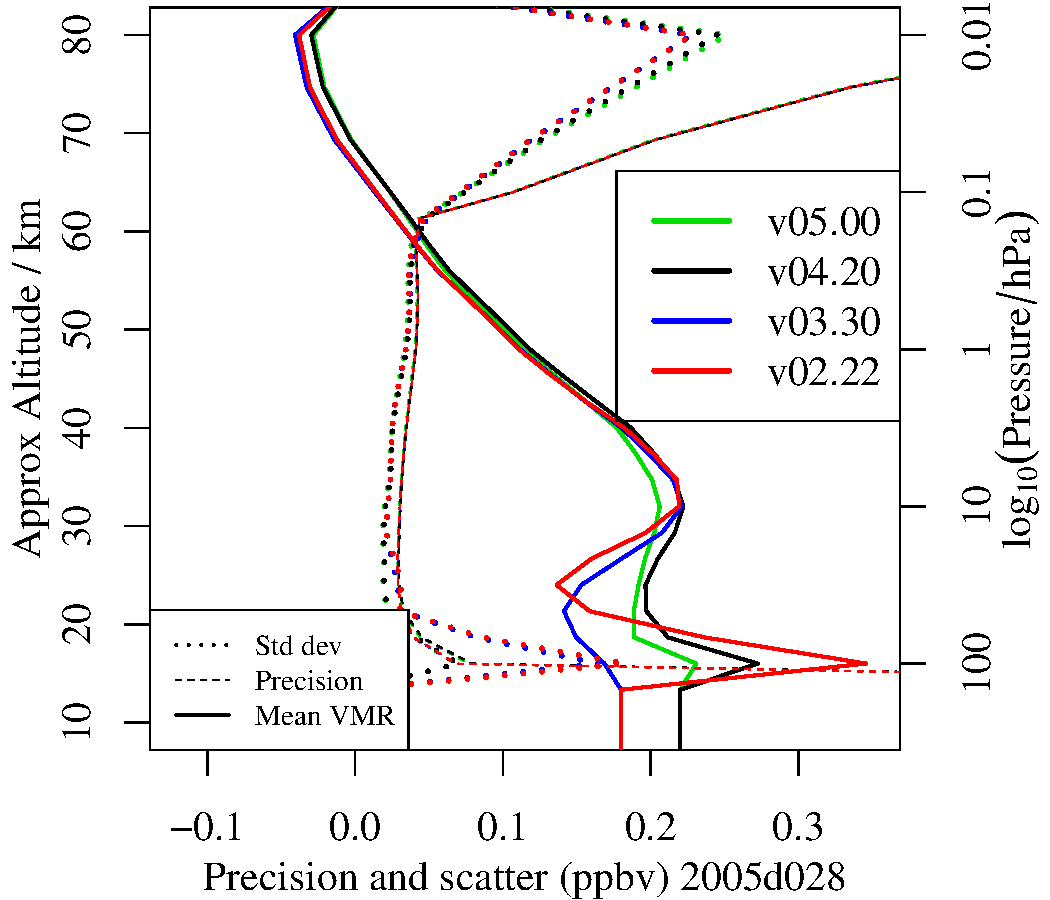
\includegraphics[width=0.495\textwidth]{figures/hcn-prec-fig-eq-2005d028}\hfill%
%   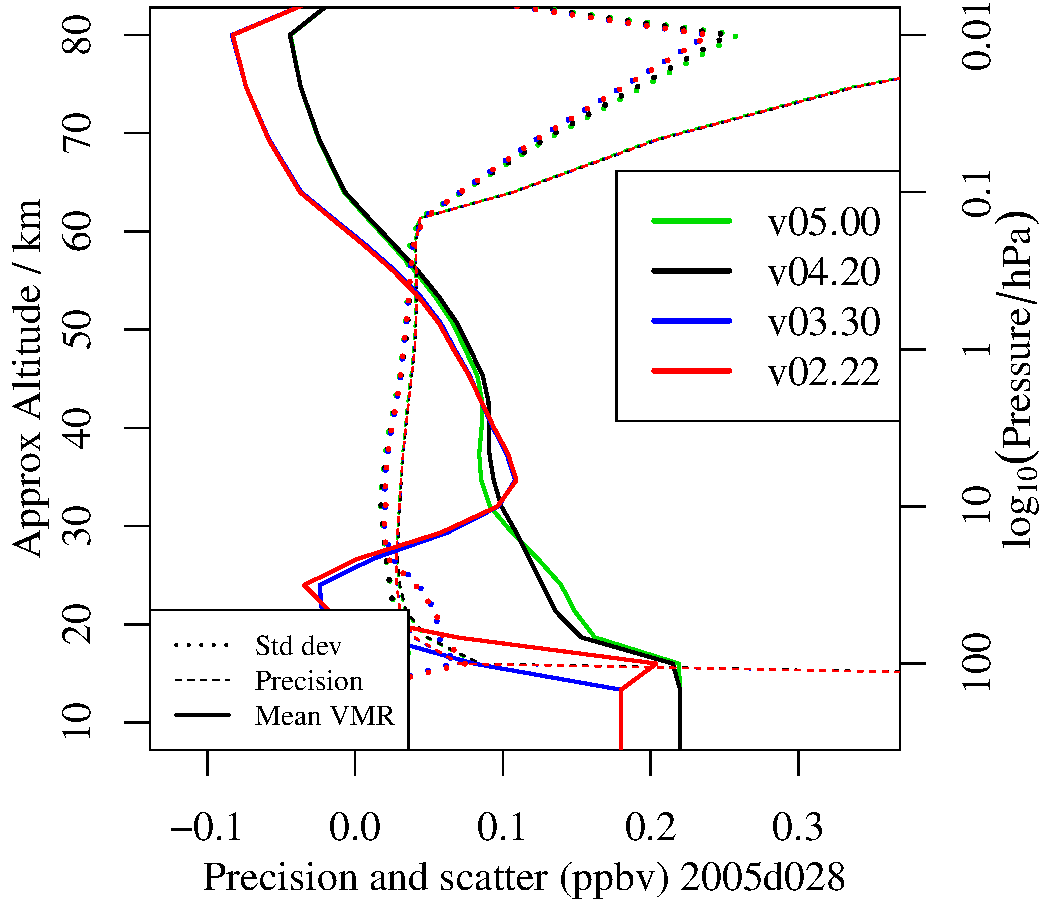
\includegraphics[width=0.495\textwidth]{figures/hcn-prec-fig-NP-2005d028}
%   \caption{Estimated precision {\tt L2gpPrecision} and observed standard deviation for MLS \thisv (orange), \prevv (green), v4.x (black), v3.x (blue) and v2.x (red) HCN\@. The data shown are all profiles within 20\degsym\ of the equator (left) and 70\degsym N--83\degsym N (right) for 28 January, 2005.  Mean mixing ratio (VMR) profiles are shown for comparison. Between 3 and 10\,hPa, \thisv and \prevv depart from the three earlier versions. At altitudes below 10\,hPa, all five versions are different, but v2.x and v3.x are less realistic than v4.x, \prevv, and \thisv.}
%   \label{fig:HCNPrecision}
% \end{figure}

\begin{figure}
  \centering%
  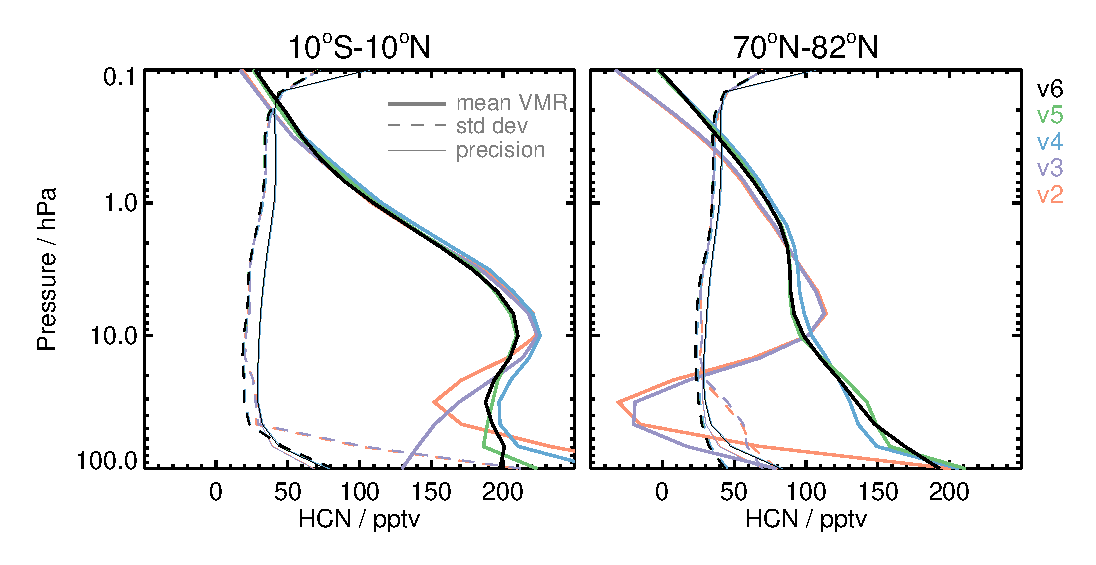
\includegraphics[width=0.9\textwidth]{figures/hcn_prof}
  \caption{Estimated precision {\tt L2gpPrecision} (thin lines) and observed standard deviation (dashed lines) for MLS \thisv (black), \prevv (green), v4.x (blue), v3.x (purple) and v2.x (red) HCN\@. The data shown are for the 10\degsym\,S to 10\degsym\,N (left) and 70\degsym\,N--82\degsym\,N (right) for 28 January, 2005.  Mean volume mixing ratio (VMR) profiles are shown for comparison. Between 3 and 10\,hPa, \thisv and \prevv depart from the three earlier versions. Below 10\,hPa, all five versions are different, but v2.x and v3.x are less realistic than v4.x, \prevv, and \thisv.}
  \label{fig:HCNPrecision}
\end{figure}


\subsection{Accuracy}

The accuracy of the HCN product has not been assessed in detail because a cursory inspection revealed that \vii and \viii HCN had extremely large systematic errors in the lower stratosphere. These errors are much smaller in \viv.  In \prevv and \thisv the errors are improved over those in \viv in some places and somewhat worse in others, while being far better than in earlier versions. Some comparisons with ACE-FTS data are shown in Figure~\ref{fig:HCNvsACE}. At 21\,hPa and higher altitudes the two instruments agree well, with MLS versions \prevv and \thisv agreeing better with ACE-FTS than \viv. In the tropics, the two instruments agree well in the 32--68\,hPa range apart from a constant systematic error. At middle and high latitudes, the MLS data differ considerably from ACE-FTS in a long-term (\mytexttilde10-year) average; the differences include a decrease at the lowest altitudes. However, the seasonal and interannual variability show many similarities between the two instruments. The MLS data in the lower stratosphere can therefore be used with caution; comparison with ACE-FTS data is advisable. In the upper stratosphere, the values are in line with current understanding of the chemistry of HCN\@. Comparison to historical values suggests an accuracy of no worse than 50\%. 

\begin{figure}
% 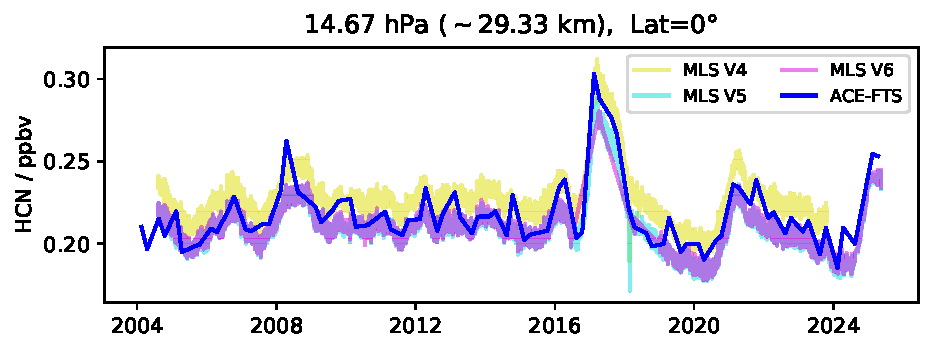
\includegraphics[width=0.82\textwidth]{figures/mls_ace_HCN_0_14-67.pdf}\\
% 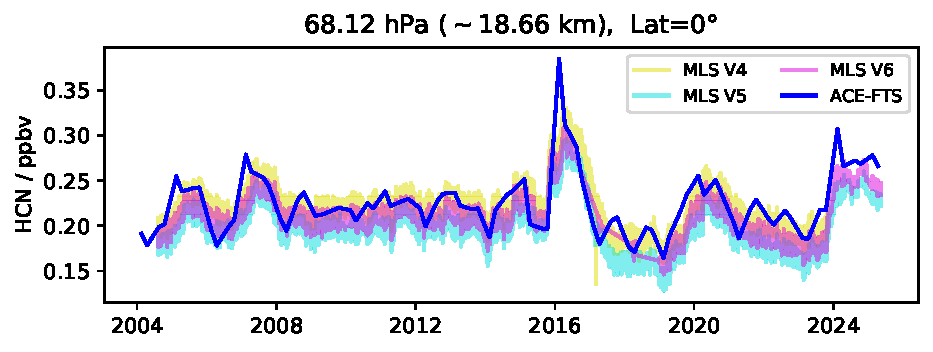
\includegraphics[width=0.82\textwidth]{figures/mls_ace_HCN_0_68-12.pdf}\\
% 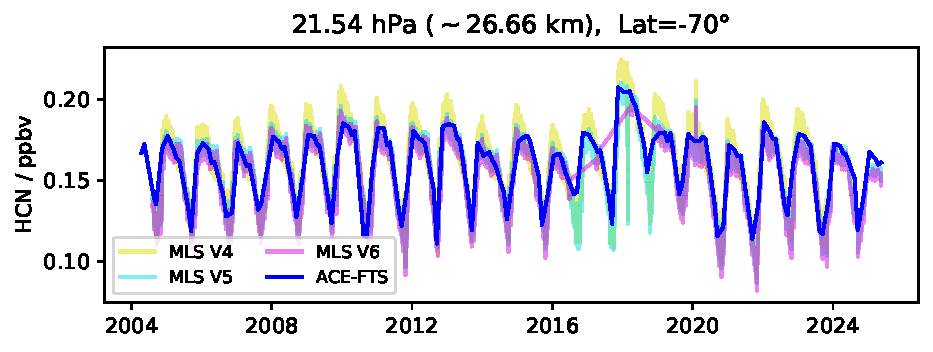
\includegraphics[width=0.82\textwidth]{figures/mls_ace_HCN_-70_21-54.pdf}\\
% 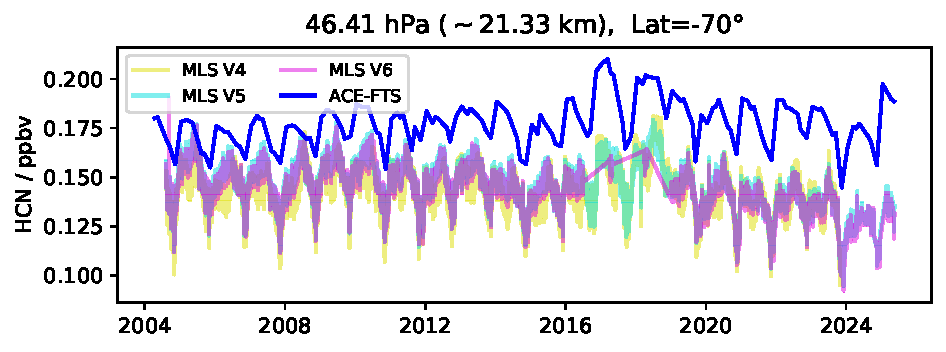
\includegraphics[width=0.82\textwidth]{figures/mls_ace_HCN_-70_46-41.pdf}
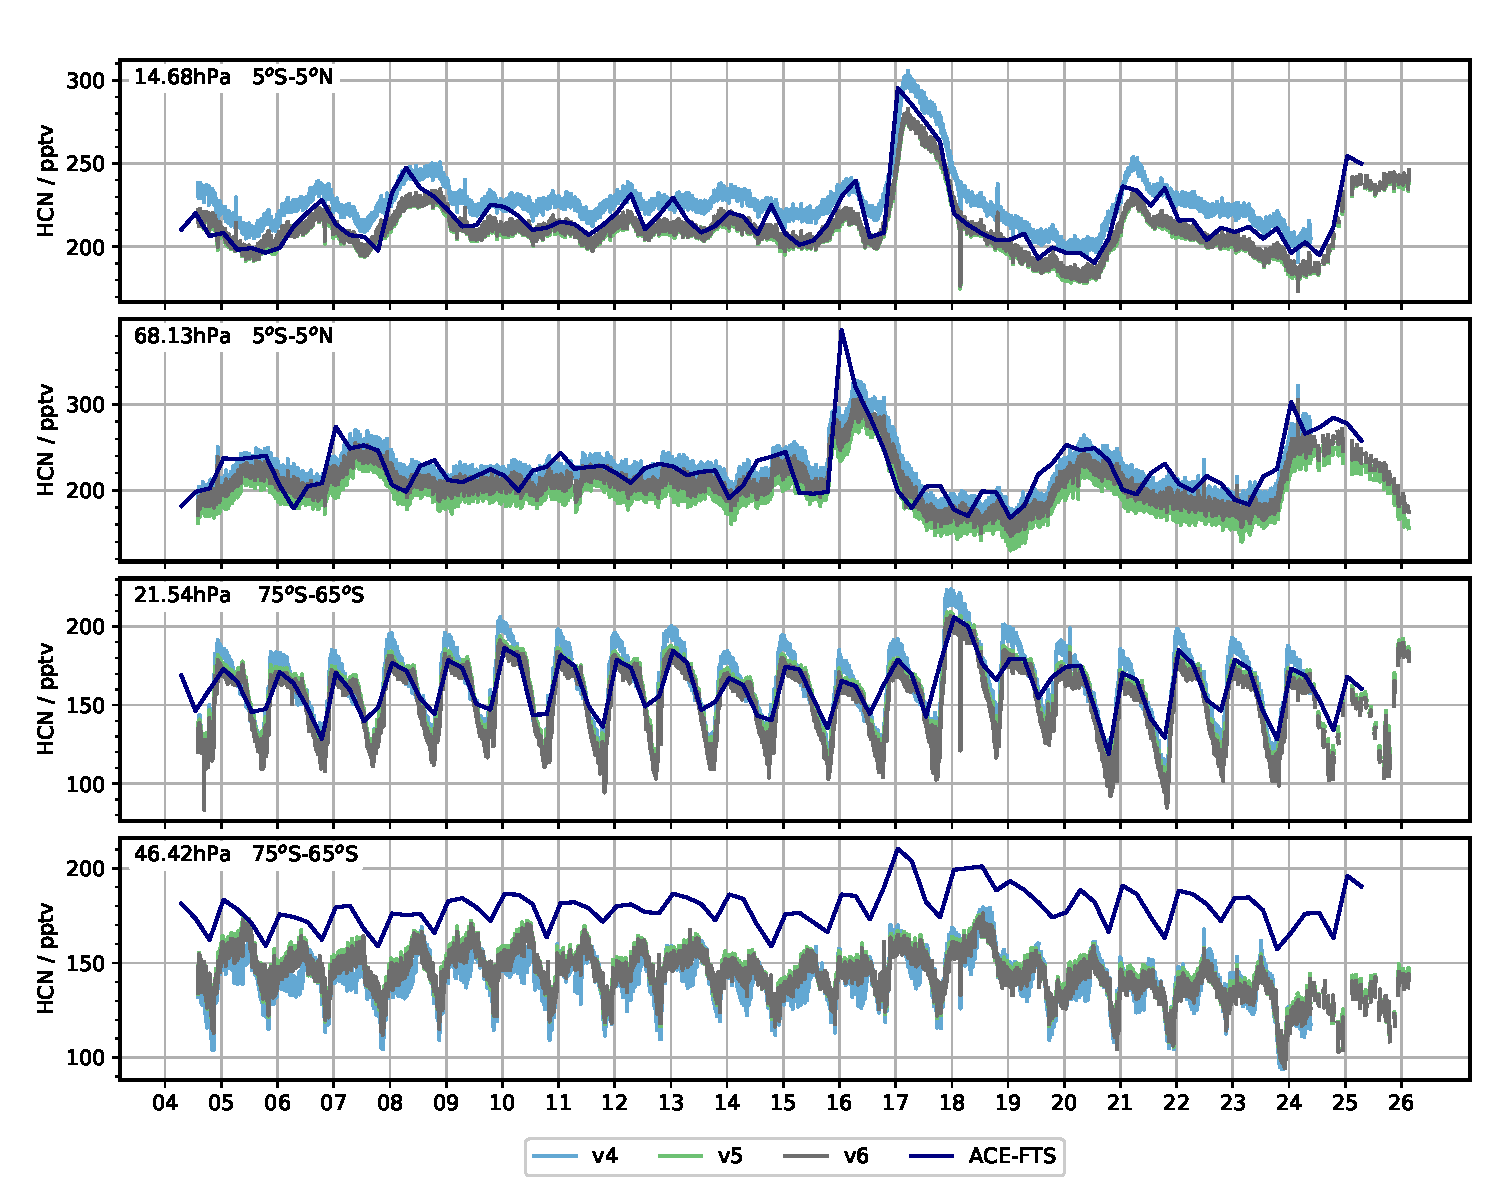
\includegraphics[width=0.9\textwidth]{figures/HCN_timeseries.pdf}
\caption{\label{fig:HCNvsACE} Daily time series of HCN at selected latitudes and pressure levels from MLS versions \viv, \prevv, and \thisv, with seasonal ACE-FTS version~5.3 for comparison.  }
\end{figure}

\begin{nofloatpages}
\subsection{Data screening}
\label{sec:HCNScreening}
\begin{description}
  \item[Pressure range:] \screeningrule{21--0.1\,hPa} \standardrangestatement\ Data in the 68\,hPa to 32\,hPa range may prove to be usable after further validation. \standardprecisionrule \evenstatusrule
  \item[Clouds:] \screeningrule{Clouds have no impact; profiles with non-zero even values of \texttt{Status} are suitable for use.} As HCN is only generally recommended in regions unaffected by clouds, profiles which have either, both, or neither of the cloud flags set may be used.
  \item[Quality:] \qualityrule{0.2} Values of \texttt{Quality} are usually near 1.5; occasional lower values do not seem correlated with unusual profiles, but we suggest as a precaution that only profiles with \texttt{Quality} $> 0.2$ be used. Typically this will eliminate only 1--2\% of profiles.
    %% Number of rejected profiles remains small in V5
  \item[Convergence:] \convergencerule{2.0} This should eliminate any chunks that have obviously failed to converge (typically only 1--2\% of the total).
    %% Number of rejected profiles remains small in V5
\end{description}
\end{nofloatpages}

\subsection{Artifacts}

There are no obvious artifacts within 21-0.1\,hPa recommended pressure range. At 68–32\,hPa, the data may be usable with caution for qualitative studies, and comparison with ACE-FTS measurements is recommended.

% \subsection{Desired improvements for future data version(s)}

% Hopefully it will prove possible to make further improvements to the retrieval of HCN in the lower stratosphere.

\begin{table}
% The precision and scatter are essentially identical in all of versions 4, 5 and 6, so this table is not changed from earlier versions of this document
  \caption{Summary of Aura MLS \thisv HCN Characteristics}
  \vspace{\tablecaptionsep}
  \label{tab:HCNSummary}
    \begin{minipage}{\linewidth}
    \renewcommand{\thefootnote}{\thempfootnote}
  \centering\begin{tabular}{ccccl}
  \toprule
  \parbox[m]{18mm}{\bfseries\centering Pressure\\ hPa} &
  \parbox[m]{22mm}{\bfseries\centering {Resolution\\ V $\times$ H%
  \footnote{Vertical and along-track horizontal resolutions; cross-track horizontal resolution is \mytexttilde9\,km.} \\ km}} &
  \parbox[m]{22mm}{\bfseries\centering Single-Profile\\ Precision%
  \footnote{The precision shown is the estimated precision (\texttt{L2gpPrecision}); the observed scatter is about 80\% of this value.} \\pptv} &
  \parbox[m]{20mm}{\bfseries\centering Accuracy \\ pptv} &
  \parbox[m]{40mm}{\bfseries Comments}\\
  \midrule
  $< 0.1$     & ---             &  --- &  ---      & Unsuitable for scientific use\\
  1--0.1      & 12 $\times$ 500 & 50   & 5         & \\
  21--1       & 10 $\times$ 300 & 40   & 15        & \\
  68--21      & 10 $\times$ 300 & 40   & 60        &  Use with caution\\
  100         & 10 $\times$ 300 & 50   & 130       &  Unsuitable for scientific use\\
  $> 100$     &                 &      &           &  Not Retrieved\\
  \bottomrule
\end{tabular}
\end{minipage}
\end{table}

\speciestitle{Nitric Acid}{HNO\cs3}{HNO\cs3}
\begin{description}
\item[Useful range:] 215\,--\,1.5\,hPa (1.0\,hPa under enhanced conditions)
\item[Contact:] Gloria Manney, \email{manney@nwra.com}
\end{description}

\subsection*{Introduction}

The quality and reliability of the Aura MLS v2.2 HNO\cs3 measurements
were assessed in detail by \citet{SanteeEtal07hno3}.  The HNO\cs3 in
\thisv has been greatly improved over that in version v2.2; in particular,
a low bias through much of the stratosphere (especially evident at
levels with pressure greater than or equal to 100~hPa) has been largely
eliminated.  Figure~\ref{fig:zmv2v3diffs} shows an example of typical
differences between v2.2 and \thisv HNO\cs3\@.  Improvement in HNO\cs3
resulted from indirect effects of adding interline interference terms to
the O\cs3 line shape model, an updated CO line width parameter, using a
different 240 GHz channel configuration for retrieving HNO\cs3, and a
change the manner in which continuum signals are accounted for (see
\ref{sec:V3vsV2Overview}); these changes contribute approximately
equally to the HNO\cs3 improvement.  However, an unfortunate side effect
of the change to continuum handling is that it is more adversely
affected by clouds, causing spikes in the retrieval of 240-GHZz products
including HNO\cs3.  In addition, it also appears that the new continuum
treatment has led to a noisier HNO\cs3 product in the UTLS than that in
v2.2.  Lower \thisv values in Figure~\ref{fig:zmv2v3diffs} in the tropics
at the lowest levels result largely from these effects.

The MLS \thisv HNO\cs3 data are scientifically useful over the range 215
to 1.5\,hPa; values at 1\,hPa are also expected to be scientifically
useful under conditions of enhanced HNO\cs3 in the upper stratosphere,
but should be used with caution and in consultation with the MLS team.
HNO\cs3 values in the upper stratosphere, at 3.2 through 1.0\,hPa, are
frequently very low and may require averaging (this will usually be the
case at 1.5 and 1\,hPa, where the values are also noisier than at lower
levels), but during periods of enhancement in the upper stratosphere,
coherently evolving atmospheric signals with realistic morphology are
seen in individual daily maps.  The standard HNO\cs3 product is derived
from the \mbox{240-GHz} retrievals at pressures equal to or greater than
22\,hPa and from the \mbox{190-GHz} retrievals for lesser pressures.
The \texttt{Quality} and \texttt{Convergence} information included in
the standard HNO\cs3 files are from the \mbox{240-GHz} retrievals, and
\emph{apply only to pressures 22\,hPa or greater} (see the data
screening discussion below).

A summary of the precision and resolution (vertical and horizontal) of
the \thisv HNO\cs3 measurements as a function of altitude is given in
Table~\ref{tab:HNO3Summary}.  The impact of various sources of
systematic uncertainty was quantified for v2.2, and it is expected that
these estimates will be similar for \thisv.  Table~\ref{tab:HNO3Summary}
also includes estimates of the potential biases and scaling errors in
the measurements compiled from the v2.2 uncertainty analysis (to be
updated for \thisv at a later date).  The overall uncertainty for an
individual data point is determined by taking the root sum square (RSS)
of the precision, bias, and scaling error terms (for averages, the
single-profile precision value is divided by the square root of the
number of profiles contributing to the average).  More details on the
precision, resolution, and accuracy of the MLS \thisv HNO\cs3 measurements
are given below.

\begin{figure}
\dontincludegraphics[angle=90,width=\linewidth]%
{figures/InspectZMContour_HNO3--v2-2_HNO3--v3-3_2005m08_LatPress-All}
\caption{V2.2 (top left) and v3.3 (top right) zonal mean HNO\cs3 for
  August~2005, and differences (v3.3\,$-$\,v2.2) expressed in ppbv (bottom
  left) and percent (bottom right).}
\label{fig:zmv2v3diffs}
\end{figure}


\subsection*{Resolution}
\onestandardavk{HNO3}{HNO\cs3}%

The resolution of the retrieved data can be described using `averaging
kernels' \citep[e.g.,][]{Rodgers00}; the two-dimensional nature of the
MLS data processing system means that the kernels describe both vertical
and horizontal resolution.  Smoothing, imposed on the retrieval system
in both the vertical and horizontal directions to enhance retrieval
stability and precision, reduces the inherent resolution of the
measurements.  Consequently, the vertical resolution of the \thisv HNO\cs3
data, as determined from the full width at half maximum of the rows of
the averaging kernel matrix shown in Figure~\ref{fig:AvkHNO3}, is
3\,--\,4\,km through most of the useful range, degrading to \texttildelow5\,km
at 22\,hPa and some levels in the upper stratosphere (see
Table~\ref{tab:HNO3Summary}).  Note that the averaging kernels for the
215 and 316\,hPa retrieval surfaces overlap over most of their depth,
indicating that the 316\,hPa retrieval provides little independent
information.  Figure~\ref{fig:AvkHNO3} also shows horizontal averaging
kernels, from which the along-track horizontal resolution is determined
to be 450\,--\,500\,km over most of the vertical range, improving to
250\,--\,300\,km between 15 and 4.6\,hPa, and degrading to
600\,--\,750\,km at 1.5 and 1\,hPa.  The cross-track resolution, set by
the widths of the fields of view of the \mbox{190-GHz} and
\mbox{240-GHz} radiometers, is \texttildelow10\,km.  The along-track separation
between adjacent retrieved profiles is 1.5\degsym\ great circle angle
(\texttildelow165\,km), whereas the longitudinal separation of MLS
measurements, set by the Aura orbit, is 10\degsym\,--\,20\degsym\ over
low and middle latitudes, with much finer sampling in the polar regions.

\subsection*{Precision}

\begin{figure}
\centering\dontincludegraphics[width=8.4cm]{figures/ComparePrecision2PanelHNO3}
\caption{Precision of the (left) v3.3 and (right) v2.2 MLS HNO\cs3
  measurements for four representative days (see legend).  Solid lines
  depict the observed scatter in a narrow equatorial band (see text);
  dotted lines depict the theoretical precision estimated by the
  retrieval algorithm.}
\label{fig:PrecProf}
\end{figure}

The precision of the MLS HNO\cs3 measurements is estimated empirically
by computing the standard deviation of the profiles in the
20\degsym-wide latitude band centered around the equator, where natural
atmospheric variability should be small relative to the measurement
noise.  Because meteorological variation is never completely negligible,
however, this procedure produces a upper limit on the precision-related
variability.  As shown in Figure~\ref{fig:PrecProf}, the observed
scatter in the \thisv data is \texttildelow0.6\,--\,0.7\,ppbv throughout the range
from 100 to 3.2\,hPa, below and above which it increases sharply.  The
scatter is essentially invariant with time, as seen by comparing the
results for the different days shown in Figure~\ref{fig:PrecProf}.

The single-profile precision estimates cited here are, to first order,
independent of latitude and season, but it should be borne in mind that
the large geographic variations in HNO\cs3 abundances gives rise to wide
range `signal to noise' ratios.  At some latitudes and altitudes and in
some seasons, HNO\cs3 abundances are smaller than the single-profile
precision, necessitating the use of averages for scientific studies.  In
most cases, precision can be improved by averaging, with the precision
of an average of $N$ profiles being 1/$\sqrt{N}$ times the precision of
an individual profile (note that this is not the case for averages of
successive along-track profiles, which are not completely independent
because of horizontal smearing).

The observational determination of the precision is compared in
Figure~\ref{fig:PrecProf} to the theoretical precision values reported
by the Level~2 data processing algorithms.  Although the two estimates
compare very well between 100 and 32\,hPa, above 22\,hPa the predicted
precision substantially exceeds the observed scatter.  This indicates
that the a priori information and the vertical smoothing applied to
stabilize the retrieval are influencing the results at the higher
retrieval levels.  Because the theoretical precisions take into account
occasional variations in instrument performance, the best estimate of
the precision of an individual data point is the value quoted for that
point in the L2GP files, but it should be borne in mind that this
approach overestimates the actual measurement noise at pressures less
than 22\,hPa.  Conversely, the observed scatter at pressures higher than
100\,hPa is considerably larger than the theoretical precision.  This is
related to the spikes and increased noise in the UTLS in \thisv versus
v2.2 HNO\cs3 mentioned above.  Procedures for screening outliers in this
region are discussed below.

\subsection*{Accuracy}

The effects of various sources of systematic uncertainty (e.g.,
instrumental issues, spectroscopic uncertainty, and approximations in
the retrieval formulation and implementation) on the MLS v2.2 HNO\cs3
measurements were quantified through a comprehensive set of retrieval
simulations; results for \thisv, to be completed at a later date, are
expected to be similar.  The results of the v2.2 uncertainty analysis
are summarized in Table~\ref{tab:HNO3Summary}; see
\citet{SanteeEtal07hno3} for further details of how the analysis was
conducted and the magnitude of the expected biases, additional scatter,
and possible scaling errors each source of uncertainty may introduce
into the data.  In aggregate, systematic uncertainties are estimated to
induce in the HNO\cs3 measurements biases that vary with altitude
between $\pm$0.5 and $\pm$2\,ppbv and multiplicative errors of
$\pm$5\,--\,15\% through most of the stratosphere, rising to
\mbox{\texttildelow$\pm$30\%} at 215\,hPa and \texttildelow50\% at and above 2.2\,hPa.
These uncertainty estimates are generally consistent with the results of
comparisons with correlative datasets, as discussed briefly below.

\subsection*{Data screening -- all data}
\label{sec:HNO3screening}

\begin{description}
\item[Pressure range:] \screeningrule{215\,--\,1.5\,hPa}
  \standardrangestatement
\standardprecisionrule
\evenstatusrule
\end{description}
\subsection*{Data screening -- upper troposphere, lower stratosphere
  (pressures of 22\,hPa or greater)}

The \texttt{Quality} and \texttt{Convergence} fields included in the
standard HNO\cs3 files are appropriate for use in screening at levels at
and below (that is, pressures greater than) 22\,hPa.  For those levels:

\begin{description}
\item[Quality:] \qualityrule{0.5}

  This threshold for \texttt{Quality} typically excludes \texttildelow2\,--\,4\% of
  HNO\cs3 profiles on a daily basis; it is a conservative value that
  potentially discards a significant fraction of ``good'' data points
  while not necessarily identifying all ``bad'' ones.

\item[Convergence:] \convergencerule{1.4}

  On a typical day this threshold for \texttt{Convergence} discards a
  very small fraction of the data, but on occasion it leads to the
  elimination of \texttildelow0.5\,--\,1\% of the HNO\cs3 profiles.
\item[Clouds:] \screeningrule{Clouds impact HNO\cs3 data in the UTLS,
    see discussion below and the discussion on `outliers' that follows.}

  Nonzero but even values of \texttt{Status} indicate that the profile
  has been marked as questionable, typically because the measurements
  may have been affected by the presence of thick clouds.  Globally
  \texttildelow10\,--\,15\% of profiles are identified in this manner, with the
  fraction of profiles possibly impacted by clouds rising to
  \texttildelow25\,--\,35\% on average in the tropics.  Clouds generally have
  little influence on the stratospheric HNO\cs3 data.  In the lowermost
  stratosphere and upper troposphere, however, thick clouds can lead to
  spikes in the HNO\cs3 mixing ratios in the equatorial regions.

  Therefore, it is recommended that at and below 68\,hPa, in addition to
  performing the `outlier screening' described below, all profiles with
  nonzero values of Status be discarded because of the potential for
  cloud contamination.  While this will reject some profiles that are
  probably not significantly impacted by cloud effects, it does
  eliminate a significant number of unphysical profiles that are not
  flagged by the outlier screening.

\item[Outliers:] \screeningrule{Alternative screening approaches in the
    UTLS remove outliers while reducing `false positives'}

  Outliers in \thisv HNO\cs3 at levels between 316 and 100 (sometimes to
  68) hPa frequently appear as highly negative mixing ratios at the
  lowest several retrieval levels, often as part of oscillatory profiles
  with unrealistically high values at higher altitudes.  A simple
  procedure is recommended to screen such profiles based on eliminating
  all profiles with large negative mixing ratios at pressure levels
  between 316 and 68\,hPa.  Through extensive examination of data
  screened in this way, flagging profiles that have either HNO\cs3 vmr
  less than $-$2.0\,ppbv at 316\,hPa or less than $-$1.6\,ppbv at any
  level between 215 and 68\,hPa eliminates most of the troublesome
  outliers, including those with positive vmr spikes overlying the
  negative ones that are directly flagged by these criteria.  This
  screening procedure is recommended for any studies focusing on the
  UTLS\@. That it effectively removes most of the suspect profiles that
  are not eliminated by requiring Status to be zero was evaluated as
  described in the following paragraphs:

  We compared the outlier screening method described above with a
  procedure based on using MLS cloud information: If the MLS ice water
  content (IWC) at 147\,hPa is greater than 0.003\,g/m$^3$ (indicating
  the presence of some cloud) for a profile, that profile, and the
  immediately adjacent ones along the orbit track are flagged (adjacent
  profiles are flagged assuming that the 1-D nature of the IWC retrieval
  versus the 2-D nature of the HNO\cs3 retrieval results in some
  uncertainty in the relative location of the cloud signal with respect
  to the trace gas profile).  Figure~\ref{fig:outlierfraction} shows the
  fraction of points eliminated by this procedure and the simpler
  recommended procedure based on direct identification of unphysical
  mixing ratios; the simpler procedure that is recommended compares very
  favorably with the more rigorous procedure based on cloud information:
  Each procedure eliminates a similar fraction of profiles (4\%
  globally, 15\% in the tropics), and is effective for removing most of
  the outliers.  Screening using MLS IWC as described here could be used
  (or compared with the recommended procedure) in analyses that are
  expected to be especially sensitive to the exact values in the
  tropical UTLS, but is not needed to obtain a high-quality HNO\cs3
  dataset in most cases.

  Figure~\ref{fig:outlierprofs} shows an example of the results of
  screening profiles by each of the \texttt{Quality},
  \texttt{Conver\-gence} and the recommended outlier flagging on a typical
  `bad' day (i.e., one with a relatively large number of outliers).  The
  \texttt{Quality} screening removes many of the profiles that are
  strongly negative at the bottom, and most or all of the remainder of
  these are flagged by the outlier screening; many of these profiles are
  oscillatory, so this screening also removes most or all of the strong
  positive outliers (typically at 147\,hPa).  Most of the profiles
  flagged by any of the criteria are in the tropics, as expected; the
  figure indicates that, at southern hemisphere high latitudes, low
  values of HNO\cs3 associated with the denitrified polar vortex are not
  triggering the outlier flagging.  As is often (but not always) the
  case, it is not clear in this example that the profiles flagged only
  by \texttt{Convergence} are unphysical or extreme.
 
\end{description}

\subsection*{Data screening -- upper stratosphere (pressures of 15\,hPa
  or less)}

The above screening criteria {\it should not be used} for 15\,hPa and
higher altitudes, as they result in filtering profiles for which all
quality indicators are good when the \texttt{Quality} and
\texttt{Convergence} values are properly taken from the 190-GHz HNO\cs3
information, and not filtering ones with indications of poor quality.
For any studies focusing on the upper stratosphere, it is highly
recommended that the user read from the \texttt{L2GP-DGG} files to
obtain the appropriate \texttt{Quality} and \texttt{Convergence} values
for the 190-GHz HNO\cs3 (from the \texttt{HNO3-190} swath), and use them
to apply the following screening criteria:
 
\begin{description}
\item[Clouds:] \screeningrule{Profiles where the \texttt{Status} field
    for \texttt{HNO3-190} has a non-zero even number can be used without
    restriction.} Clouds generally have little influence on the
  stratospheric HNO\cs3 data at these altitudes.

\item[Quality:] \screeningrule{Only profiles with a value of the
    \texttt{Quality} field for \texttt{HNO3-190} (see
    section~\ref{sec:StatusQuality}) \emph{greater} than 1.0 should be
    used in scientific study.}

  This threshold for \texttt{Quality} typically excludes
  \texttildelow1\,--\,3\% of HNO\cs3 profiles on a daily basis; it is a
  conservative value that potentially discards a significant fraction of
  ``good'' data points while not necessarily identifying all ``bad''
  ones.

\item[Convergence:] \screeningrule{Only profiles with a value of
    the \texttt{Convergence} field (see section~\ref{sec:StatusQuality})
    for the \texttt{HNO3-190} product \emph{less} than 1.6 should be
    used in investigations.}

  On a typical day this threshold for \texttt{Convergence} discards
  \texttildelow0.5\,--\,1.5\% of the HNO\cs3 profiles.

\item[Outliers:] For levels at and above (pressures less than) 4.6\,hPa,
  especially at 2.2\,hPa and above, some profiles show vertically
  oscillatory behavior in conditions where HNO\cs3 is very low.  The
  \texttt{Quality} and \texttt{Convergence} criteria defined above, when
  used together, eliminate many of these profiles; screening using both
  of these thresholds is thus particularly important.
\end{description}

\begin{figure}
\centering\dontincludegraphics[width=8.4cm]{figures/HNO3_frac_screened_by_lat_2}
\caption{Fraction of profiles flagged by two suggested outlier screening
  procedures for the UTLS as a function of latitude for \thisv data
  during 2006.}
\label{fig:outlierfraction}
\end{figure}

\begin{figure}
\centering\dontincludegraphics[width=16.4cm]{figures/profqual_utls2005d230}
\caption{HNO\cs3 profiles on 18~Aug~2005 color-coded by screening.
  Cyan profiles have \texttt{Quality} less than 0.5, olive-green
  \texttt{Convergence} greater than 1.4, and red both \texttt{Quality}
  less than 0.5 and \texttt{Convergence} greater than 1.4.  Orange
  profiles are those flagged by the simple screening procedure described
  above (using large negative mixing ratios at high pressures) after the
  profiles that failed \texttt{Quality} and/or \texttt{Convergence}
  tests were removed.  Black profiles are all those remaining (the
  `good' profiles) after the screening.  The left panels show all
  individual profiles in the day; the right panels show the means in
  each category, with the standard deviation shown as bars and the range
  as dotted lines.  The horizontal line is at 22\,hPa, above which
  HNO\cs3 is from the 190-GHz radiometer and thus not appropriately
  screened by these criteria.  The four pairs of panels show all
  profiles (top left), profiles between $-$20 and 20\degsym\ latitude (top
  right), profiles between $-$90 and $-$50\degsym\ latitude (bottom left) and
  profiles between 50 and 90\degsym\ latitude.}
\label{fig:outlierprofs}
\end{figure}

\subsection*{Review of comparisons with other datasets}


V3.3 / v3.4 HNO\cs3 has been compared with correlative datasets from a
variety of different platforms.  A consistent picture has emerged of
much closer agreement in \thisv than v2.2 with HNO\cs3 measurements from
ground-based, balloon-borne, and satellite instruments, especially in
the upper troposphere through the mid-stratosphere where MLS v2.2
HNO\cs3 mixing ratios were uniformly low by 10\,--\,30\%.  Example
comparisons with balloon-borne measurements
(Figures~\ref{fig:ftsumnerhno3comps} and \ref{fig:gbmshno3comps}) and
Atmospheric Chemistry Experiment-Fourier Transform Spectrometer
satellite measurements (Figure~\ref{fig:acehno3comps}) are shown.  The
GBMS ground-based measurements (Figure~\ref{fig:gbmshno3comps})
highlight the change from v2.2 to \thisv; in all years, MLS HNO\cs3
values increased from v2.2 to \thisv over most/all of the altitude
range, and in 2004\,--\,2005 and 2006\,--\,2007 show much closer
agreement with GBMS measurements; in all years, MLS HNO\cs3 agrees with
GBMS within the error bars.  The 2005\,--\,2006 winter was characterized
by extremely strong dynamical activity, which may contribute to the
different relationship between MLS and GBMS measurements in that year;
detailed GBMS/MLS comparisons are described by \citet{FiorucciEtal13}.

The Ft.\ Sumner balloon comparisons also show much improved agreement
between HNO\cs3 measured by several instruments with \thisv MLS data
(compare Figure~\ref{fig:ftsumnerhno3comps} with Figures~11 and 12 of
\citet{SanteeEtal07hno3}).  ACE-FTS comparisons also show improvements,
with the low bias in MLS virtually eliminated over the entire altitude
range shown in the top panel comparing with ACE-FTS v2.2 data in
May~2008 (other months show similar results) -- this can be contrasted
with Figure~25 of \citet{SanteeEtal07hno3}, which showed a low bias in
MLS v2.2 data with respect to ACE v2.2 throughout the useful altitude
range.

ACE-FTS HNO\cs3 reprocessed with v3.0 shows improvements in the UTLS,
and is useful up to \texttildelow60\,km. The bottom panels of
Figure~\ref{fig:acehno3comps} show a comparison of ACE-FTS v3.0 data with MLS \thisv
data during January 2005, indicating good agreement throughout the
altitude range.

Preliminary comparisons also indicate closer agreement for version 3
HNO\cs3 with aircraft measurements in the UTLS than for version 2.

\begin{figure}
\centering\dontincludegraphics[width=13.4cm]{figures/ftsumnerallhno3}
\caption{Comparisons with balloon-borne measurments at Ft. Sumner in
  2004 (left) and 2005 (right).  (Top panels) Path traversed by
  measurements from the balloon-borne MkIV (blue triangles) and FIRS-2
  (green and orange crosses represent two separate profiles) instruments
  during the flights from Ft.\ Sumner, NM, on 23\,--\,24~September 2004
  (left) and 20\,--\,21~September~2005 (right).  Measurement tracks from
  nearby MLS orbits are also shown (open circles).  The two MLS data
  points closest to the balloon measurements in time and space are
  indicated by red squares, with the closer one denoted by a filled
  symbol; the 500-km radius around the closest MLS point is overlaid in
  black.  (Bottom) Profiles of HNO\cs3 from MLS (red squares), MkIV
  (blue triangles), and FIRS-2 (green and orange crosses), corresponding
  to the symbols in the top panel.  Error bars represent the estimated
  precisions of each instrument, taken from the data files.  }
\label{fig:ftsumnerhno3comps}
\end{figure}

\begin{figure}
\vspace*{-0.5cm}
\centering\dontincludegraphics[width=13.4cm]{figures/gbmsallhno3}
\caption{Comparisons with GBMS balloon measurements.  (Top) Averages of
  all GBMS (blue) profiles and closest MLS (v2.2 in red, \thisv in
  green) coincidences at Testa Grigia (45.9$\degsym$N, 7.7$\degsym$E)
  during the 2004\,--\,2005, 2005\,--\,2006, and 2006\,--\,2007 winters;
  bars are standard deviation of the mean.  (Center) Differences between
  mean profiles shown in top panels (GBMS\,--\,MLS) in ppbv; (bottom)
  same differences, expressed as percentages.  }
\label{fig:gbmshno3comps}
\end{figure}

\begin{figure}
\centering\dontincludegraphics[width=15.4cm]{figures/acehno3compsv2v3}
\caption{Comparisons with ACE-FTS v2.2 measurements during May~2008
  (top) and ACE-FTS v3.30 measurements during Jan~2005 (bottom).  (left)
  Global ensemble mean profiles of the collocated matches for both
  instruments (MLS, red; ACE-FTS, blue). (middle) Mean percentage
  difference profiles between the two measurements (MLS\,--\,ACE-FTS)
  (cyan); standard deviation about the mean differences (Observed SD;
  orange) and the percentage root sum square of the precisions on both
  instrument measurements (Expected SD; magenta).  (right) As in Figure
  13 (middle) except plotted in mixing ratio.}
\label{fig:acehno3comps}
\end{figure}

\subsection*{Desired improvements for future data version(s)}
\begin{itemize}
\item Reduce noise/spikes in UTLS and in upper stratosphere.
\item Minimize the impact of thick clouds on the retrievals to further
  improve the HNO\cs3 measurements in the upper troposphere and
  lowermost stratosphere.
\end{itemize}

\begin{table*}
\caption{Summary of Aura MLS \thisv HNO\cs3 Characteristics}\vspace{0.5ex}
\label{tab:HNO3Summary}
\begin{minipage}{\linewidth}
  \renewcommand{\thefootnote}{\thempfootnote}
  \centering\begin{tabular}{cccccl} \toprule
\parbox[m]{18mm}{\bfseries\centering{Pressure\\ / hPa}} &
\parbox[m]{24mm}{\bfseries\centering{Resolution\\ \mbox{V $\times$ H}%
\footnote{Horizontal resolution in along-track direction.} \\ / km}} &
\parbox[m]{18mm}{\bfseries\centering{Precision%
\footnote{Precision on individual profiles, determined from observed
 scatter in the data in a region of minimal atmospheric variability.} \\/ ppbv}} &
\parbox[m]{20mm}{\bfseries\centering{Bias\\uncertainty%
\footnote{Values should be interpreted as \mbox{2-$\sigma$} estimates
 of the probable magnitude.}\\ / ppbv}} &
\parbox[m]{20mm}{\bfseries\centering{Scaling\\uncertainty%
\footnotemark[\value{mpfootnote}]\\/ \%}} &
\textbf{Comments} \\
%
\midrule
%
0.68\,--\,0.001 & ---  & ---    & ---    & --- & Unsuitable for scientific
  use\\
%
1.0 & 4 $\times$ 650\,--\,750  & $\pm$1.2 & $\pm$0.5 & $\pm$50\% & Caution, averaging
recommended \\
%
1.5 & 4.5 $\times$ 550\,--\,600 & $\pm$1.0  & $\pm$0.5 & $\pm$50\% & Averaging recommended \\
%
2.1 & 5 $\times$ 500 & $\pm$0.9  & $\pm$1.0 & $\pm$50\% & \\
%
3.2 & 4.5 $\times$ 400 & $\pm$0.7  & $\pm$0.5  & $\pm$10\,--\,15\% & \\
%
15\,--\,6.8  & 3\,--\,4 $\times$ 250\,--\,300 & $\pm$0.7 & $\pm$1\,--\,2  &
  $\pm$10\% & \\
%
22 & 5 $\times$ 450 & $\pm$0.7 & $\pm$1\,--\,2 &
$\pm$10\% & \\
%
100\,--\,32  & 3\,--\,4 $\times$ 350\,--\,400 & $\pm$0.7 & $\pm$0.5\,--\,1 &
$\pm$5\,--\,10\% & \\
%
147        & 3.5  $\times$ 400\,--\,450      & $\pm$0.8 &
$\pm$0.5  & $\pm$15\% & \\
%
215        & 3.5\,--\,4 $\times$ 500      & $\pm$1.2 & $\pm$1    &
\texttildelow$\pm$30\% & \\
%
316        & ---      & ---    & ---    & --- & Unsuitable for
scientific use\\
%
1000\,--\,464  & ---      & ---    & ---    & --- & Not retrieved\\
%
\bottomrule
\end{tabular}\par
\end{minipage}
\end{table*}

%%% Local Variables: 
%%% mode: latex
%%% TeX-master: "v4-x-report"
%%% End: 


\speciestitle{Peroxy Radical}{\ch{HO2}}{HO2}{%
  \item[Useful range:] 22--0.046\,hPa
  \item[Product lead:] Luis Mill\'an \email{Luis.F.Millan@jpl.nasa.gov}}

\subsection{Introduction}
MLS observes \ch{HO2} emission lines within the 640-GHz radiometer. A description of \ch{HO2} data quality, precision, systematic errors, and validation for an earlier version, \vii, is given by \citet{PickettEtal:2006:Validation}. An early validation using v1.5 software is also described by \citet{PickettEtal:2006:Validation}. The estimated uncertainties, precisions, and resolution for \thisv \ch{HO2} are summarized below in Table~\ref{tab:HO2Summary}.  

An algorithm to retrieve daily zonal means of \ch{HO2} over an extended vertical range by first averaging the radiances has been developed by the MLS team \citep{MillanEtal:2015}. This alternative dataset provides daytime and nighttime \ch{HO2} measurements across the stratosphere and mesosphere. This dataset and associated documentation is available from the GES-DISC with the product short name ``\texttt{ML3DZMHO2}''.

\subsection{Resolution}

Figure~\ref{fig:AvkHO2} shows the \ch{HO2} averaging kernel for daytime at 70\degsym N and the Equator. The latitudinal variation in the averaging kernel is very small. The vertical resolution for pressures greater than 0.1\,hPa is generally about 5\,km.

\subsection{Precision}

A typical \ch{HO2} profile and the associated precisions (for both \prevv and \thisv) are shown in Figure~\ref{fig:HO2profiles}. The profile is shown in both volume mixing ratio (vmr) and density units. All MLS data are reported in vmr for consistency with the other retrieved molecules. However, use of density units (10\cp{6}\,cm\cp{$-$3}) reduces the apparent steep gradient of the \ch{HO2} vertical profile, allowing one to see the profile with more detail. The nighttime \ch{HO2} profile is expected to exhibit a narrow layer near the altitudes of the nighttime OH layer at \mytexttilde82\,km \citep{PickettEtal:2006:NightOH}, which is not shown in Figure~\ref{fig:HO2profiles} since MLS \ch{HO2} data are not recommended for altitudes above 0.046\,hPa (\mytexttilde70\,km). Precisions are such that an \ch{HO2} zonal average within a 10\degsym\ latitude bin can be determined with better than 10\% relative precision with 20 days of data (\mytexttilde2000 samples) for most pressure levels over 22--0.046\,hPa.

\oneverticalavk{HO2}{\ch{HO2}}%

\begin{figure}
  \begin{center}
    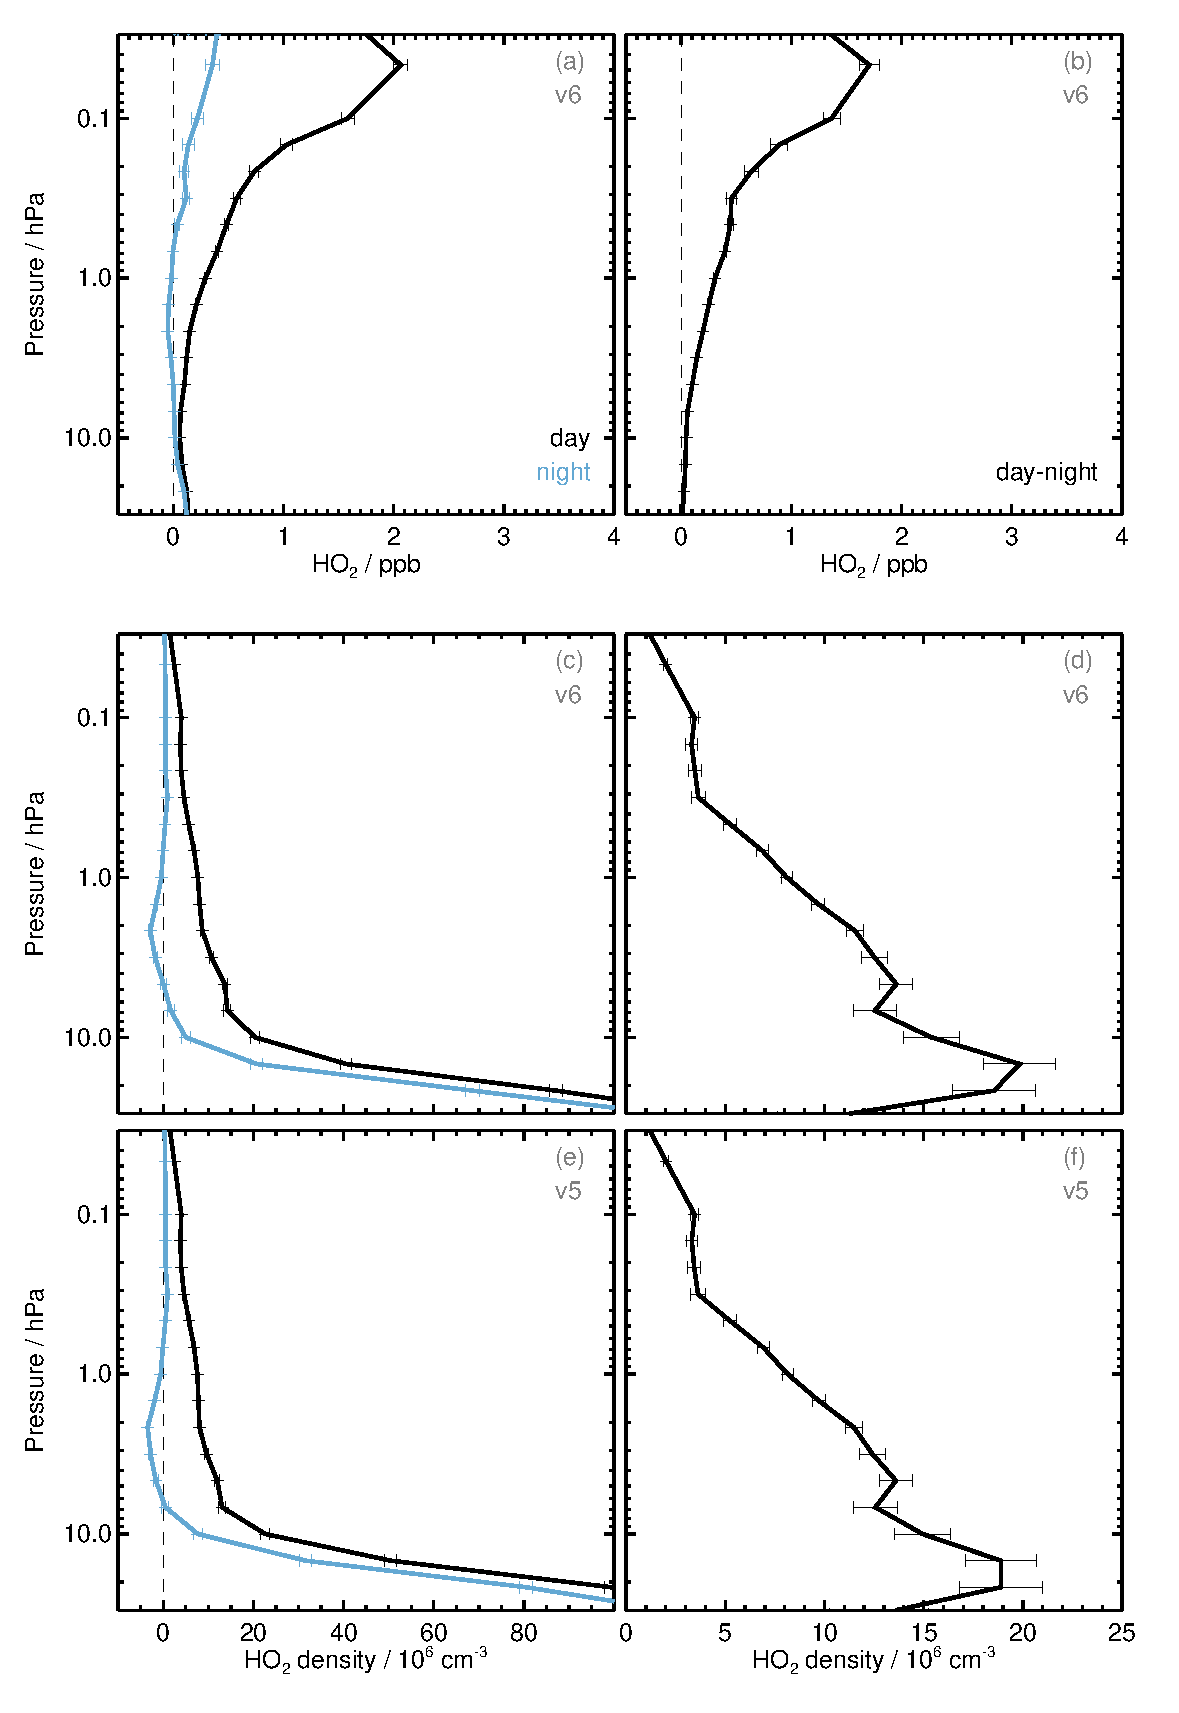
\includegraphics[width=0.8\linewidth]{figures/plot_ho2zmv6.pdf}%
  \end{center}
  \caption{Monthly zonal mean of retrieved \ch{HO2} and its estimated precision (horizontal error bars) for January 2005 averaged over 29\degsym N to 39\degsym N. Panel (a) shows \thisv \ch{HO2} vmr vs.\ pressure for day (black) and night (blue). Panel (b) shows the same data plotted as a day/night difference (note that a day/night difference is required for \ch{HO2} for all pressure levels). Panel (c) shows the same data in (a) converted into density units. Panel (d) shows the day-night differences for the data in panel (c). Panels (e) and (f) are equivalent to (c) and (d) but using \prevv data.}
  \label{fig:HO2profiles}
\end{figure}

\subsection{Accuracy}

Table~\ref{tab:HO2Summary} summarizes the accuracy expected for \thisv \ch{HO2}. The effect of each identified source of systematic error on MLS measurements of radiance has been quantified and modeled \citep{ReadEtal:2007}. These quantified effects correspond to either 2$\sigma$ estimates of uncertainties in each MLS product or an estimate of the maximum reasonable uncertainty based on instrument knowledge and/or design requirements. The \ch{HO2} bias can be minimized by taking day/night differences over the entire recommended pressure range. The overall uncertainty is the square root of the sum of squares of the precision and accuracy.

\begin{nofloatpages}
\subsection{Data screening}
\label{sec:HO2Screening}

\begin{description}
  \item[Pressure range:] \screeningrule{22--0.046\,hPa} \standardrangestatement \standardprecisionrule \evenstatusrule
  \item[Quality:] \screeningrule{MLS \thisv \ch{HO2} data can be used irrespective of the value of the \texttt{Quality} field.}
  \item[Convergence:] \convergencerule{1.1} 
\end{description}
\end{nofloatpages}

\subsection{Artifacts}
Currently, there are no known artifacts in the \ch{HO2} product. The primary limitations are its precision and its narrow recommended altitude range. That said, the alternative daily zonal mean dataset (short name: ``\texttt{ML3DZMHO2}'') offers three distinct improvements over the standard MLS \ch{HO2} product: (1) an extended pressure range, enabling measurements of the mesospheric maximum that occurs near 0.02\,hPa, (2) expanded latitudinal coverage, allowing measurement at the poles, where the \ch{HO2} is located, and (3) nighttime \ch{HO2} estimates.

\subsection{Review of comparisons with other datasets}
\ch{HO2} data from MLS \vii software have been validated with two balloon-borne remote-sensing instruments. Details of the comparison are given by \citet{PickettEtal:2006:Validation}. Comparisons between \vii and \thisv show no differences large enough to alter results of previous validation studies.

\begin{table}
  \caption{Summary of Aura MLS \thisv \ch{HO2} Characteristics}
  \vspace{\tablecaptionsep}
  \label{tab:HO2Summary}
  \begin{minipage}{\linewidth}
    \small\centering\begin{tabular}{ccccl}
\toprule
\tableheaderbox{Pressure\\ \\hPa} &
\tableheaderbox{Vertical\\resolution\\km} &
\tableheaderbox{Single-Profile\\Precision\footnote{Precision (1$\sigma$) on individual profiles as reported in the L2GP files.}\\ \\10\cp6 cm\cp{$-$3}} &
\tableheaderbox{Day--night\\accuracy\\10\cp6 cm\cp{$-$3}} &
\textbf{Comments} \\
\midrule
 $<$ 0.03  & ---   & ---               & ---  &  Unsuitable for scientific use\\
 0.046     & 10    & 4                 & 0.01 &  Use day--night difference \\
 0.10      & 7     & 8                 & 0.3  &  Use day--night difference \\
 1.0       & 5     & 11                & 0.5  &  Use day--night difference \\
 10        & 4     & 56                & 15   &  Use day--night difference \\
 $>$ 22    & ---   & ---               & ---  &  Unsuitable for scientific use\\
\bottomrule
\end{tabular}
  \end{minipage}
\end{table}

\speciestitle{Hypochlorous Acid}{HOCl}{HOCl}{%
  \item[Useful range:] 10--2.2\,hPa
  \item[Contact:] Lucien Froidevaux, \email{Lucien.Froidevaux@jpl.nasa.gov}}

\subsection{Introduction}

There has been very little change in the \thisv HOCl retrieval results since \prevv, and any small changes are well within the somewhat large estimated accuracies (systematic uncertainties). We provide below sample mean HOCl distributions for the \thisv and \prevv data versions, and their differences. Otherwise, previous information regarding this species remains largely unchanged; the main points are mentioned here mainly for new data users.

The HOCl retrieval is quite noisy for individual profiles and HOCl data require some averaging (e.g., in 10\degsym\ zonal means for one or more weeks) to get useful precision of better than 10\,pptv, in comparison to typical upper stratospheric HOCl abundances of 100--150\,pptv. Table~\ref{tab:HOClSummary} summarizes the MLS HOCl resolution, precision, and accuracy estimates for the upper stratosphere. More discussion and a brief validation summary are given in the following sections, along with data screening recommendations. For trend results regarding MLS HOCl in the upper stratosphere, see \citep{FroidevauxEtal:2021:HOCl}.

An algorithm to retrieve daily zonal means of HOCl by first averaging the radiances has been developed by the MLS team, building on the work described in \citet{MillanEtal:2012} and \citet{MillanEtal:2015} for BrO and HO\cs2, respectively. This dataset reduces the variability slightly and will be available for \thisv from the GSFC DISC soon; it is expected to be very similar to the (\prevv) HOCl dataset used by \citep{FroidevauxEtal:2021:HOCl}. 

\subsection{Changes from \prevv}
There were no significant algorithmic changes relating directly to HOCl for the \thisv retrievals. However, given the small level of HOCl spectral radiance signal, the retrieved HOCl abundances can be sensitive, indirectly, to even minor changes in the retrieval system, such as changes in temperature or tangent pressure. In \prevv, small changes that likely contributed to HOCl differences included some changes to nitric acid in the R4 (640\,GHz) retrievals, in conjunction with (or tied to) changes from other bands (e.g., via differences in tangent pressure, temperature, and water vapor), and slight changes to a priori values for certain species (nitric acid, ozone, and water vapor).

The background observed in the 640-GHz radiances includes emissions from N\cs2, O\cs2, and H\cs2O. There are laboratory-based and ground-based models for the continuum absorptions that are the basis for the MLS absorption model \citep[][and references therein]{PardoEtal:2001}. These models were tested against MLS extinction measurements from the wing channels in the 640-GHz radiometer. The latitude dependence of this extinction was found to agree better with the expected moist plus dry continuum extinction values if the dry and moist continuum functions were scaled by factors close to 20$\%$; however, this aspect is no different than what was done in the previous data version.

A comparison plot showing zonal average upper stratospheric HOCl contours (from 10 to 2\, hPa) and differences between the two data versions for a typical month (April, 2009) is provided in Figure~\ref{fig:MLSv5v6HOClContour}. The average \thisv HOCl abundances are slightly larger than the \prevv retrievals, typically by about 10 to 15\, pptv (or 10 to 15$\%$); this has removed some of the small negative values that often occurred in \prevv HOCl contour plots at the highest southern latitudes, between 5 and 10\,hPa.  The estimated precision values are essentially unchanged from \prevv.

\begin{figure}
  \centering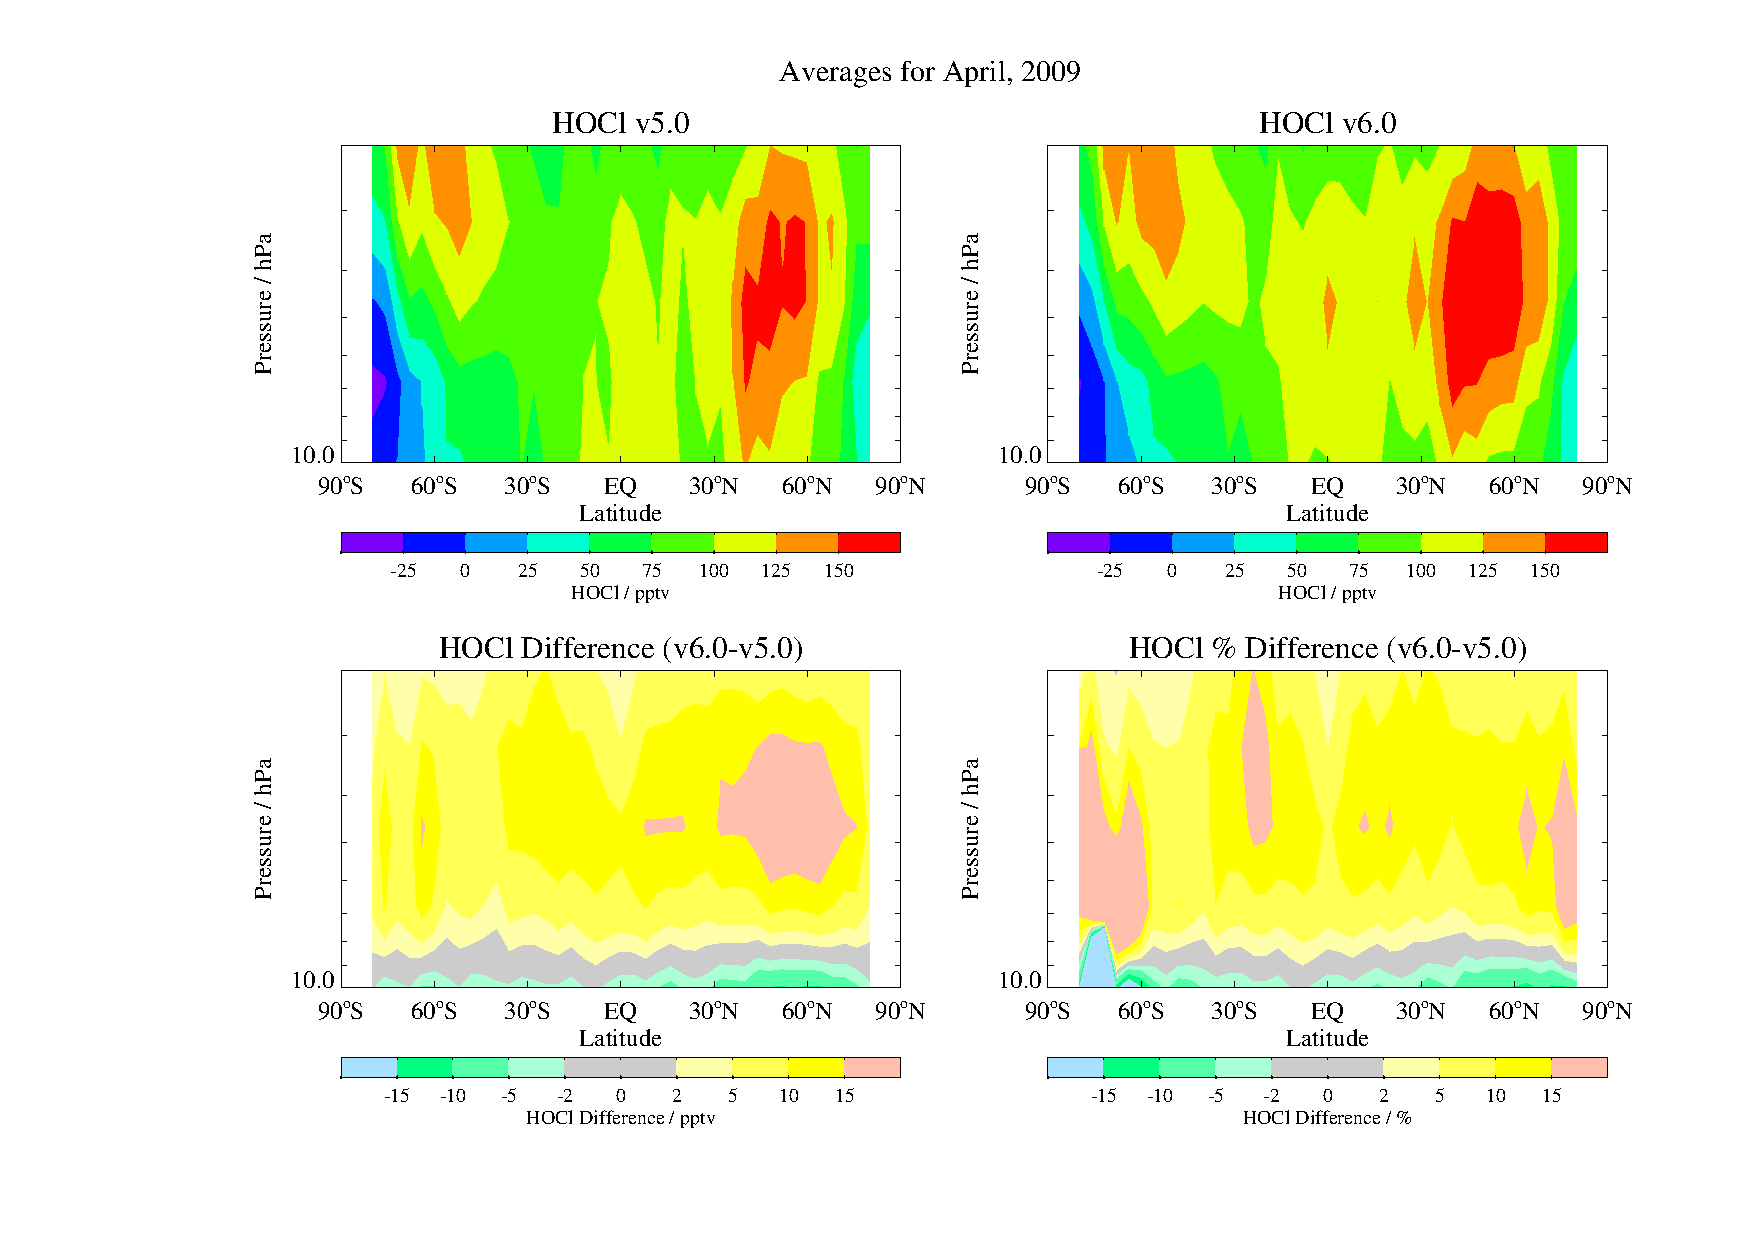
\includegraphics[angle=0,width=1.\linewidth]{figures/Fig-HOCl_v6v5_ZmContours_Difs.pdf}
  \caption{Zonal averages for upper stratospheric MLS HOCl profiles during April, 2009, showing the MLS \prevv HOCl mixing ratio contours (top left panel), the \thisv contours (top right panel), and their differences in pptv (\thisv minus \prevv, bottom left panel) and percent (\thisv minus \prevv versus \prevv, bottom right panel). }
  \label{fig:MLSv5v6HOClContour}
\end{figure}

\subsection{Resolution}
\oneverticalavk{HOCl}{HOCl}%

Based on the width of the averaging kernels shown in Figure~\ref{fig:AvkHOCl}, the vertical resolution for upper stratospheric HOCl is \mytexttilde6\,km (significantly worse than the 640-GHz radiometer vertical field of view width of 1.4\,km). This reflects the choice of smoothing constraints for HOCl which favor precision over vertical resolution.

\subsection{Precision}

The estimated single-profile precision reported by the Level~2 software is about 300 to 400\,pptv in the upper stratosphere. A more useful number of 5 to 10\,pptv is quoted in Table~\ref{tab:HOClSummary} for the typical precision of a 10\degsym\ weekly zonal means for this product.

\subsection{Accuracy}

The accuracy estimates shown in Table~\ref{tab:HOClSummary} come from a formal quantification of the combined effects of possible systematic errors in MLS calibration, spectroscopy, etc.\ on the HOCl retrievals \citep{ReadEtal:2007}. These values are intended to represent $2\sigma$ estimates of accuracy. The largest contributors to possible errors for HOCl are contaminant species, gain compression, and sideband ratio uncertainties. The Table gives a range of error estimates (for now, these are based on \prevv but they are not expected to change significantly). 
%The average changes for upper stratospheric HOCl between \prevv and \thisv are well within the quoted accuracy estimates (which may be somewhat conservative). The HOCl signal becomes too small compared to the systematic uncertainties to allow for reliable retrievals at pressures larger than 10 hPa.

\subsection{Data screening}
\label{sec:HOClScreening}
\begin{description}
  \item[Pressure range:] \screeningrule{10--2.2\,hPa} \standardrangestatement\ Artifacts (negative averages) for pressures larger than about 10\,hPa make this product unsuitable for use in the lower stratosphere. Regarding the topmost altitude range, the sensitivity to \emph{a priori} increases rapidly at pressures of 1\,hPa or less; we continue to recommend the use of (average) HOCl values only up to 2.2\, hPa. \standardprecisionrule \evenstatusrule

  \item[Quality field:] \screeningrule{Only profiles with a value of the \texttt{Quality} field \emph{greater} than 1.2 should be used.}
  This criterion removes profiles with the poorest radiance fits, typically less than 0.2$\%$ of the daily profiles. For HOCl, this screening correlates well with the poorly converged sets of profiles (see below); we recommend the use of both the \texttt{Quality} and \texttt{Convergence} fields for data screening.

  \item[Convergence field:] \screeningrule{Only profiles with a value of the \texttt{Convergence} field \emph{less} than 1.05 should be used.} For the vast majority of profiles (99$\%$ or more for most days), this field is less than 1.05. Nevertheless, on occasion, sets of profiles (typically one or more groups of ten profiles, retrieved as a `chunk') have this \texttt{Convergence} field set to larger values, and should be discarded.

  \item[Clouds:] \cloudsokrule

\end{description}

\subsection{Review of comparisons with other datasets}

The MLS HOCl retrievals exhibit the expected morphology in monthly mean latitude / pressure contour plots; for example, such plots for September months from MLS compare favorably, to first-order, with results produced by the Michelson Interferometer for Passive Atmospheric Sounding (MIPAS) for September, 2002 \citep{VonClarmannEtal:2006}. MLS HOCl averages at midlatitudes are close to the results from balloon-borne infrared measurements. Generally favorable comparisons (within the error bars) have been made of the diurnal changes in upper stratospheric HOCl between Aura MLS (v3.3), other satellite datasets, and a 1-D photochemical model \citep{KhosraviEtal:2013}.

\subsection{Artifacts}
\begin{itemize}
  \item The 640-GHz radiometer bands 10 (for ClO) and 29 (for HOCl) were turned off for a few time periods in 2006 to investigate degradation issues that might affect these channels in the future. These bands were off on April 8,9, and 10, 2006, and also for April 17, 2006 (after 19:52 UT) through May 17, 2006. There are essentially no useful HOCl (or ClO) data for these time periods. The \thisv (as for previous data versions) software correctly flags these incidents with poor (odd) \texttt{Status} values (which should be screened out).
  \item There are significant artifacts in the mean values (large negative values) for HOCl in the lower stratosphere, where the use of this product is not recommended.
  \item Users should screen out the non-converged and poorest quality HOCl profiles, as such profiles (typically a very small number per day) tend to behave unlike the majority of the other MLS retrievals. See the criteria listed above.
\end{itemize}

\begin{table}
  \caption{Summary for MLS hypochlorous acid}\vspace{0.5ex}
  \label{tab:HOClSummary}
  \begin{minipage}{\linewidth}\small
    \centering\begin{tabular}{ccccccl}
\toprule
\parbox[m]{15mm}{\centering\textbf{Pressure}} &
\multicolumn{2}{c}{\parbox[m]{16mm}{\centering\textbf{Precision\footnote{Precision ($1\sigma$) 
for 1 week/10 degrees zonal means or 2 weeks/5 degrees zonal means}}}} &
\parbox[m]{24mm}{\centering\textbf{Vertical\\ Resolution\\km}} &
\multicolumn{2}{c}{\parbox[m]{16mm}{\centering\textbf{Accuracy\footnote{$2\sigma$ estimate from systematic 
uncertainty characterization tests}\\}}} 
&
\textbf{Comments} \\
\textbf{hPa} & \textbf{pptv} & \textbf{\%} & \textbf{km}& \textbf{pptv} & \textbf{\%} & \\
\midrule
1.5 or less & ---   & ---   & ---    & ---    & ---     & Unsuitable for scientific use \\ 
2.2 to 10   & 5--10 & 5--20 & 5.5--6 & 40--80 & 25--100 & Some averaging required \\ 
15 or more  & ---   & ---   & ---    & ---    & ---     & Unsuitable for scientific use \\    
\bottomrule
\end{tabular}
  \end{minipage}
\end{table}

\speciestitle{Cloud Ice Water Content}{IWC}{IWC}{%
\item[Units:] g/m\cp3
\item[Useful range:] 215\,--\,83\,hPa
\item[Contact: ] Alyn Lambert, \email{Alyn.Lambert@jpl.nasa.gov}}

\subsection{Introduction}

The MLS IWC is retrieved from cloud-induced radiances (\Tcir) of the
240-GHz window channel in a separate processing step after the
atmospheric state (Temperature and tangent height pressure) and important
gaseous species (H\cs2O, O\cs3, HNO\cs3) have been finalized in the
retrieval processing.  The derived \Tcir\ are binned onto the standard
horizontal (1.5\degsym\ along track) and vertical (12 surfaces per
decade change in pressure) grids, and converted to IWC using the modeled
\Tcir\,--\,IWC relations \citep{WuEtal:2006}.  The standard IWC profile has
a useful vertical range between 215\,--\,83\,hPa although the validation
has been conducted for a subset of the range of IWC values. IWC
measurements beyond the value ranges specified in
Table~\ref{tab:IWCSummary} are to be regarded currently as giving only
qualitative information on cloud ice.  They require further validation
for quantitative interpretation.

\subsection{Resolution}

In the IWC ranges specified in Table~\ref{tab:IWCSummary}, each MLS
measurement can be quantitatively interpreted as the average IWC for the
volume sampled. This volume has a vertical extent of \texttildelow3\,km, with
\texttildelow300\,km and 7\,km along and cross track respectively.

\subsection{Precision}

The precision values quoted in the IWC files do not represent the true
precision of the data.  The precision for a particular measurement must
be evaluated on a daily basis using the method described in the
screening section below.  The precision listed in
Table~\ref{tab:IWCSummary} reflects typical values obtained from the
method described below.

\subsection{Accuracy}

The IWC accuracy values listed in Table~\ref{tab:IWCSummary} are
estimates from comparisons of the earlier v2.2 MLS data product with
CloudSat and detailed analyses on the v2.2 error budget can be found in
\citet{WuEtal:2008}.

\subsection{Data screening}
\label{sec:IWCScreening}
\begin{description}
\item[Pressure range (215\,--\,83\,hPa):] \standardrangestatement\ The
  maximum detectable IWC is \texttildelow100\,mg/m\cp3.
\item[Use Temperature Status, Quality and Convergence:] The user is
  recommended to screen the IWC data using the \texttt{Status} field in
  the collocated temperature profile to exclude bad retrievals
  \citep{SchwartzEtal:2008:Validation}. In other words, only IWC profiles for which
  temperature \texttt{Status} is an even number should be used.
  Similarly, the users should only use IWC profiles where the
  corresponding Temperature profiles have \emph{Quality} of 0.9 or
  larger and \texttt{Convergence} less than 1.03.
\item[Other screening:] The IWC product derives from differences between
  measured radiances and those predicted assuming cloud free conditions.
  Spectroscopic and calibration uncertainties give rise to temporally
  and geographically varying biases in this difference, and hence the
  IWC product.  These biases must be iteratively identified and removed,
  using a ``$2\sigma$\,--\,$3\sigma$'' screening method, as described
  below.

\begin{enumerate}
\item Uncertainties in spectroscopy and atmospheric composition are
  manifested as residual biases in the IWC fields which should be
  identified and removed as follows.  IWC data should be averaged in a
  10\degsym\ latitude bins and outliers rejected iteratively by
  excluding measurements greater than $2\sigma$ standard deviation about
  the mean ($\mu$) of the bin. Repeat the $\sigma$ and $\mu$
  calculations after every new set of rejections.  Convergence is
  usually reached within 5\,--\,10 iterations, and the final $\sigma$ is
  the estimated precision for the IWC measurements.
\item Interpolate the final $\sigma$ and $\mu$ to the latitude of
  each measurement, and subtract $\mu$ from IWC for each measurement.
\item Finally, apply the 3$\sigma$ threshold to determine if an IWC
  measurement is statistically significant. In other words, it must have
  $\text{IWC} > \mu + 3\sigma$ in order to be considered as a
  significant cloud hit.  The $3\sigma$ threshold is needed for cloud
  detection since a small percentage of clear-sky residual noise can
  result in a large percentage of ``false alarms'' in cloud detection.
\end{enumerate}
\end{description}

\subsection{Artifacts}

At wintertime mid-to-high latitudes, strong stratospheric gravity waves
may induce large fluctuations in the retrieved tangent pressure, and
cause false cloud detection with the 2$\sigma$\,--\,3$\sigma$ screening
method. The false cloud detection seems to affect the 100\,hPa pressure
level most, as expected for such impact coming from the lower
stratosphere.

\subsection{Comparisons with other datasets}
  
Scatter plots of \thisv vs v2.2 IWC show mean biases of less than 10\%
in the pressure range 215\,--\,83\,hPa and histograms show that
the random noise in \thisv IWC is generally larger than in v2.2 (see
Figure~\ref{fig:IWC} and Table~\ref{tab:IWCSummary}). However, in
localized regions, there can be substantial differences in IWC values
between these versions that are driven by the reaction of the IWC
retrieval to the changes in \thisv UTLS H\cs2O.  These effects are largest at
pressures of 215~hPa and higher and have been verified by examining
the negative correlations between the changes in H\cs2O and IWC.

Apart from the differences noted above,
the MLS \thisv IWC is similar to the MLS v2.2 product described and
validated in \citet{WuEtal:2008}.  A revised validation paper for IWC is
not planned in the near future and users are encouraged to read
\citet{WuEtal:2008} for more information.

Comparisons between v2.2 MLS and CloudSat IWC showed good agreement with
PDF differences $<$50\% for the IWC ranges specified in
Table~\ref{tab:IWCSummary}. Comparisons with AIRS, OMI and MODIS suggest
that MLS cloud tops are slightly higher by \texttildelow1\,km than the
correlative data in general.

\begin{table}
  \caption{Summary of MLS \thisv IWC precision, accuracy, and resolution.}
\vspace{\tablecaptionsep}
\label{tab:IWCSummary}
\begin{minipage}{\linewidth} \centering\begin{tabular}{cccccc} \toprule
    \parbox{6em}{\bfseries\centering Pressure / hPa} &
    \parbox{6em}{\bfseries\centering Resolution\footnote{The along-track,
        cross-track and vertical extent, respectively of the atmospheric volume
        sampled by an individual MLS measurement.} / km} &
    \parbox{6em}{\bfseries\centering Typical precision\footnote{These are
        typical 1$\sigma$ precisions where the better values are for the
        extratropics and the poorer values for the tropics. The precision for a
        particular measurement must be evaluated on a daily basis using the
        method described in the text.} / mg/m\cp3} &
    \multicolumn{2}{c}{\parbox{12em}{\null\hfill\bfseries
        Accuracy\footnote{Estimated from comparisons with CloudSat.} /
        mg/m\cp3\hspace{8ex}\hfill\null\\%
        \null\hspace{-3ex}$<$10\,mg/m\cp3\hfill$>$10\,mg/m\cp3\hspace{4ex}\null}}
    &
    \parbox{6em}{\bfseries\centering Valid IWC range\footnote{This is the
        range where the stated precision, accuracy and resolution are
        applied. In this range MLS measurements can be quantitatively
        interpreted as the average IWC for the volume sampled. IWC values above
        this range, currently giving qualitative information on cloud ice,
        require further validation for quantitative interpretation.} \\ /
      mg/m\cp3} \\ \midrule
p$<$70 & \multicolumn{5}{c}{Unsuitable for scientific use} \\
 83 & 200$\times$7$\times$5 & 0.06\,--\,0.15     & 100\% & ---   & 0.02\,--\,50 \\
100 & 200$\times$7$\times$5 & 0.08\,--\,0.18     & 100\% & 150\% & 0.02\,--\,50 \\
121 & 250$\times$7$\times$4 & 0.08\,--\,0.24     & 100\% & 100\% & 0.04\,--\,50 \\
147 & 300$\times$7$\times$4 & 0.20\,--\,0.65 & 100\% & 100\% & 0.1\,--\,50  \\
177 & 300$\times$7$\times$4 & 0.5\,--\,2.3   & 150\% & 100\% & 0.3\,--\,50  \\
215 & 300$\times$7$\times$4 & 1.2\,--\,5.5   & 300\% & 100\% & 0.6\,--\,50  \\
p$>$260 & \multicolumn{5}{c}{Unsuitable for scientific use} \\ \bottomrule
\end{tabular}
\end{minipage}
\end{table} 
 
\begin{figure}
  \includegraphics[width=\textwidth]{figures/IWC-240-v05-00-dataqual-JUL2009-v2}
  \caption{MLS v4, v3 and v2 IWC comparisons for July 2009 at 146\,hPa
    and 100\,hPa.  (a) Left: Probability density functions (PDF) (v5,
    red; v4, blue; and v2, green) with dashed lines showing the
    corresponding noise levels (obtained by folding the negative IWC
    values about the origin) and the thin black lines representing the
    gaussian error function.  (b) Right: Scatter plots of IWC v4 vs.\ v2
    (black points) with dashed red lines indicating the 1:1 line, dashed
    yellow lines the $1\sigma$ uncertainties and the solid yellow lines are linear
    fits to the data (which lie practically on the 1:1 line).}
\label{fig:IWC}
\end{figure}

%%% Local Variables: 
%%% mode: latex
%%% TeX-master: "v5-x-report"
%%% End: 

\speciestitle[(stored as an additional swath in the \texttt{L2GP-IWC}
  file).]{Cloud Ice Water Path}{IWP}{IWP}{%
  \item[Units:] g/m\cp2
  \item[Useful range:] MLS IWP is the ice water column above \mytexttilde6\,km
  \item[Contact: ] Alyn Lambert, \email{Alyn.Lambert@jpl.nasa.gov}}

\subsection{Introduction}

MLS standard IWP is retrieved from cloud-induced radiances (\Tcir) of the 240\nobreakdash-GHz window channel at 650\,hPa tangent pressure (see Figure~\ref{fig:IWPSketch}). It represents a partial column above \mytexttilde6\,km, and is stored in the \thisv L2GP IWC file as a separate swath. For the IWP retrieval, \Tcir\ is first converted to a near horizontal slant path (with a \mytexttilde3\degsym\ elevation angle) IWP ``hIWP'', using the modeled \Tcir--hIWP relation. The hIWP is then converted to the nadir IWP at the tangent point location, and interpolated to the MLS standard horizontal grid.

As noted in Section~\ref{sec:R2DutyCycling}, since May 2024 the \mbox{190\nobreakdash-GHz} radiometer is operated only intermittently. When that radiometer is turned off, in the absence of \ch{H2O} measurements, \emph{a priori} information for \ch{H2O} (based on climatological values) is used in the derivation of the IWP data product, adversely affecting the quality. Therefore, we do not recommend the use of IWP data during the periods that the \mbox{190\nobreakdash-GHz} radiometer is turned off. Further details are given in Section~\ref{sec:IWPScreening}.

\subsection{Resolution}

In the IWP ranges specified in the summary at the end of this section, each MLS measurement can be quantitatively interpreted as the average IWP for the volume sampled. The MLS IWP volume is a vertical column above \mytexttilde6\,km, with 60\,km and 7\,km along- and cross-track extent, respectively.

\subsection{Precision}

The precision values quoted in the IWP swaths do not represent the true precision of the data. The precision for a particular measurement must be evaluated on a daily basis using the method described in the screening section below. The 3\,g/m\cp2 precision given in the summary at the end of this section reflects \emph{typical values} for MLS IWP measurements.

\subsection{Accuracy}

The IWP accuracy is \mytexttilde50\%, as estimated from comparisons of the earlier \vii MLS data product with CloudSat and detailed analyses on the \vii error budget can be found in \citet{WuEtal:2009}.

\subsection{Data screening}
\label{sec:IWPScreening}
\begin{description}
  \item[Sensitivity:] The standard IWP product has a useful sensitivity up to 200\,g/m\cp{2} where MLS measurements can be quantitatively interpreted as the average IWP for the volume sampled.
  \item[Use Temperature Status, Quality and Convergence:] The user is recommended to screen the IWP data using the \texttt{Status} field in the collocated temperature profile to exclude bad retrievals \citep{SchwartzEtal:2008:Validation}. In other words, only IWP values for which Temperature \texttt{Status} is an even number should be used. Similarly, the users should only use IWP values where the corresponding Temperature profiles have \emph{Quality} of \CheckThis 0.9 or larger and \texttt{Convergence} less than \CheckThis 1.03.
  \item[Other screening:] the user is also recommended to screen the IWP data for significant cloud hits on a daily basis using the ``2$\sigma$, $3\sigma$'' method described in the IWC section (\ref{sec:StandardIWC}). The $3\sigma$ threshold is needed for cloud detection since a small percentage of clear-sky residual noise can result in a large percentage of false alarm in cloud detection.  Note that this screening step cannot provide an adequate correction for the lack of retrieved \ch{H2O} during the periods when the \mbox{190\nobreakdash-GHz} radiometer is turned off, and so the additional screening step on \ch{H2O} \texttt{Status} given below takes precedence.
  
          \item[Additional screening on \ch{H2O} \texttt{Status}:] As noted earlier, the quality of the IWP product is degraded when the \mbox{190\nobreakdash-GHz} radiometer is turned off, since only climatological \ch{H2O} is available in lieu of retrieved \ch{H2O}. In these circumstances, the IWP values cannot be quantitatively compared to measurements taken on surrounding days or in previous years when the \mbox{190\nobreakdash-GHz} radiometer was operational. Therefore, for quantitative studies, an additional screening step is recommended, whereby the \texttt{Status} field in the collocated \ch{H2O} profile is examined to remove affected IWP data. That is, only IWP values for which the \texttt{Status} flags of the corresponding \ch{H2O} profiles are an even number should be used in quantitative studies relying on IWP measurements.    
          
          \end{description}

\subsection{Artifacts}

High-latitude high-land surface can be mistakenly detected as a cloud when the atmosphere is very dry, allowing MLS 240\nobreakdash-GHz radiances to penetrate down to the surface. Surface emission/scattering can then reduce brightness temperature. Surface effects (e.g., over the highland over Antarctica) may introduce artificial IWP values as large as 10\,g/m\cp2. In addition, the geographical location of MLS IWP is currently registered at the tangent point, which is \mytexttilde2 profiles away from the actual location of the IWP column as shown in Figure~\ref{fig:IWPSketch}. The user needs to correct this offset by replacing the IWP location with the one at two profiles earlier.

\subsection{Comparisons with other datasets}
Compared to \vii IWP the \thisv IWP values are similar and the random noise is slightly smaller than in \vii (see Figure~\ref{fig:IWP}). Apart from the differences noted above, the MLS \thisv IWP is similar to the MLS \vii product described and validated in \citet{WuEtal:2009}. A revised validation paper for IWP is not planned in the near future and users are advised to read \citet{WuEtal:2009} for more information.

Comparisons between \vii MLS and CloudSat IWP showed good agreement with PDF differences $<$50\% for the IWP range specified in the summary at the end of this section.

\subsection{Desired improvements for future data version(s)}

The IWP retrieval in \thisv is a simple first-order conversion, applied independently to each \Tcir\ measurement. Future development work on the MLS IWP retrieval should consider implementing a 2-D cloudy-sky radiative transfer model. This will allow IWP to be retrieved jointly with the \Tcir\ measurements from adjacent scans.

\subsection{Summary for IWP}
\begin{description}
  \item[IWP column bottom:] \screeningrule{6\,km (estimated from MLS radiative transfer model calculations).} The calculation of the bottom height of the IWP column depends on the tropospheric water vapor loading and on the IWP itself and is discussed in \citet{WuEtal:2009}.
  \item[Typical precision:] \screeningrule{3\,g/m\cp2 is the typical 1$\sigma$ precision.} The precision for a particular measurement must be evaluated on a daily basis using the method described in the text.
  \item[Accuracy:] \screeningrule{50\% (estimated from comparisons with CloudSat)}
  \item[Resolution:] \screeningrule{60\,km along track, 7\,km across track (the volume of air sampled by MLS)}
  \item[Valid IWP range:] \screeningrule{$\le$200\,g/m\cp2} This is the range where the stated precision, accuracy and resolution are applied. In this range MLS measurements can be quantitatively interpreted as the average IWP for the volume sampled. IWP values above this range, currently giving qualitative information on cloud ice, require further validation for quantitative interpretation.
\end{description}

\begin{figure}
  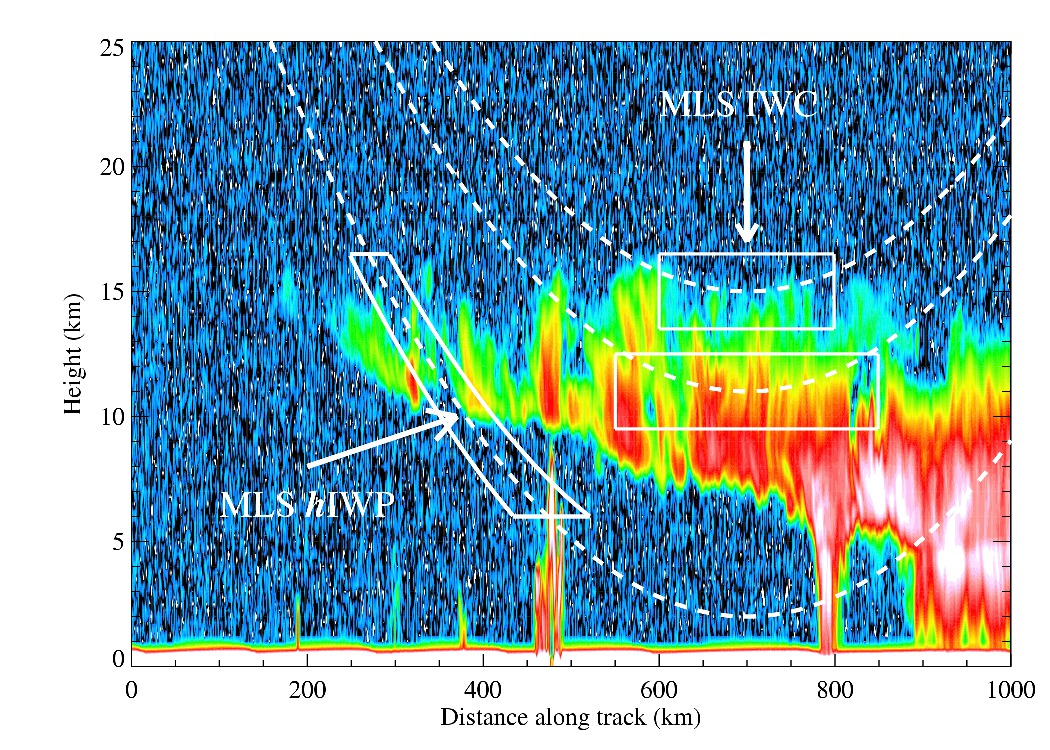
\includegraphics[width=\textwidth]{figures/iwp-figure-bitmap.jpg}
  \caption{Diagram to illustrate the MLS IWC and IWP measurement. The dashed lines are the MLS tangential beams. At high tangent heights, the beams penetrate through the limb and become sensitive to a volume-averaged IWC, whereas, at low tangent heights, the MLS beams cannot penetrate through the limb due to strong gaseous absorption and become only sensitive to a partial slant column of IWP, with a shallow (\mytexttilde3\degsym) angle, ``hIWP''.  Note that the actual volume of the air represented by hIWP is centered \mytexttilde300\,km away from the tangent point, or \mytexttilde2 profiles from the location of the nominal profile.}
  \label{fig:IWPSketch}
\end{figure}

\begin{figure}
  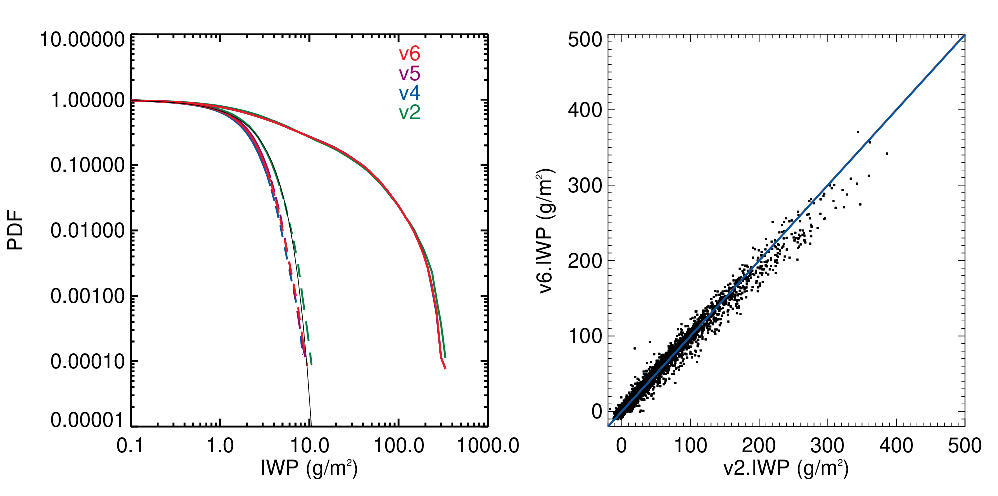
\includegraphics[width=\textwidth]{figures/IWP-240-v6-dataqual-JUN2009}
  \caption{MLS v6, v5, v4 and v2 IWP comparisons for June 2009.  (a) Left: Probability density functions (PDF) (v6 (red), v5 (purple), v4 (blue) and v2 (green)) with dashed lines showing the corresponding noise levels (obtained by folding the negative IWP values about the origin) and the thin black lines representing the gaussian error function. (b) Right: Scatter plot of IWP \thisv vs v2 (black points) with a linear fit to the data shown as a blue line and lying practically along the 1:1 line.}
  \label{fig:IWP}
\end{figure}

\speciestitle{Nitrous Oxide}{N\cs2O}{N2O}{%
\item[Useful range:] 68\,--\,0.46\,hPa
\item[Contact:] Alyn Lambert, \email{Alyn.Lambert@jpl.nasa.gov}}

\subsection{Introduction}

\subsubsection{Redefinition of the N\cs2O standard product for \thisv
  to use band 3 (190-GHz) signals}

The standard product for \thisv N\cs2O is taken from the 190-GHz
(``Core+R2'') retrieval (\texttt{N2O-190}) instead of the 640-GHz (``Core+R4B'')
retrieval (\texttt{N2O-640}) as used in previous versions.

Aging of the MLS ``band~12'' (640-GHz) signals was revealed by analysis
of housekeeping data during June-August 2013 which showed declining
output in counts, increasing radiance noise (variance) and also
increasing correlation between the band 12 radiance channels. As the
640\,GHz N\cs2O product began to show further deterioration in quality a
decision was made to turn off band 12 on August 6, 2013. Prior to that,
the level-2 processing stream for the N\cs2O standard product in v3.x
was switched to output the ``band~3'' (190-GHz, \texttt{N2O-190}) retrieval
on 7~June 2013 and later data for \texttt{N2O-640} are not recommended
for scientific use.

The 190-GHz N\cs2O data show slightly worse precision and resolution
compared to the 640-GHz retrievals. Data from \texttt{N2O-190} and
\texttt{N2O-640} have been compared from launch until the end of band 12
operations. There is a persistent high bias in \texttt{N2O-190} of
$>30\%$ at 100 hPa (although some seasonal variations are evident) and
we recommend that at this particular pressure level \texttt{N2O-190}
only be used in consultation with the MLS science team.  A smaller bias
of 5--10\% at 68\,hPa in \texttt{N2O-190} is seen compared to
\texttt{N2O-640}. From 46 to 3.2\,hPa the biases are less than 5\% (see
Figure~\ref{fig:N2O190640Comparison}).

\begin{figure}
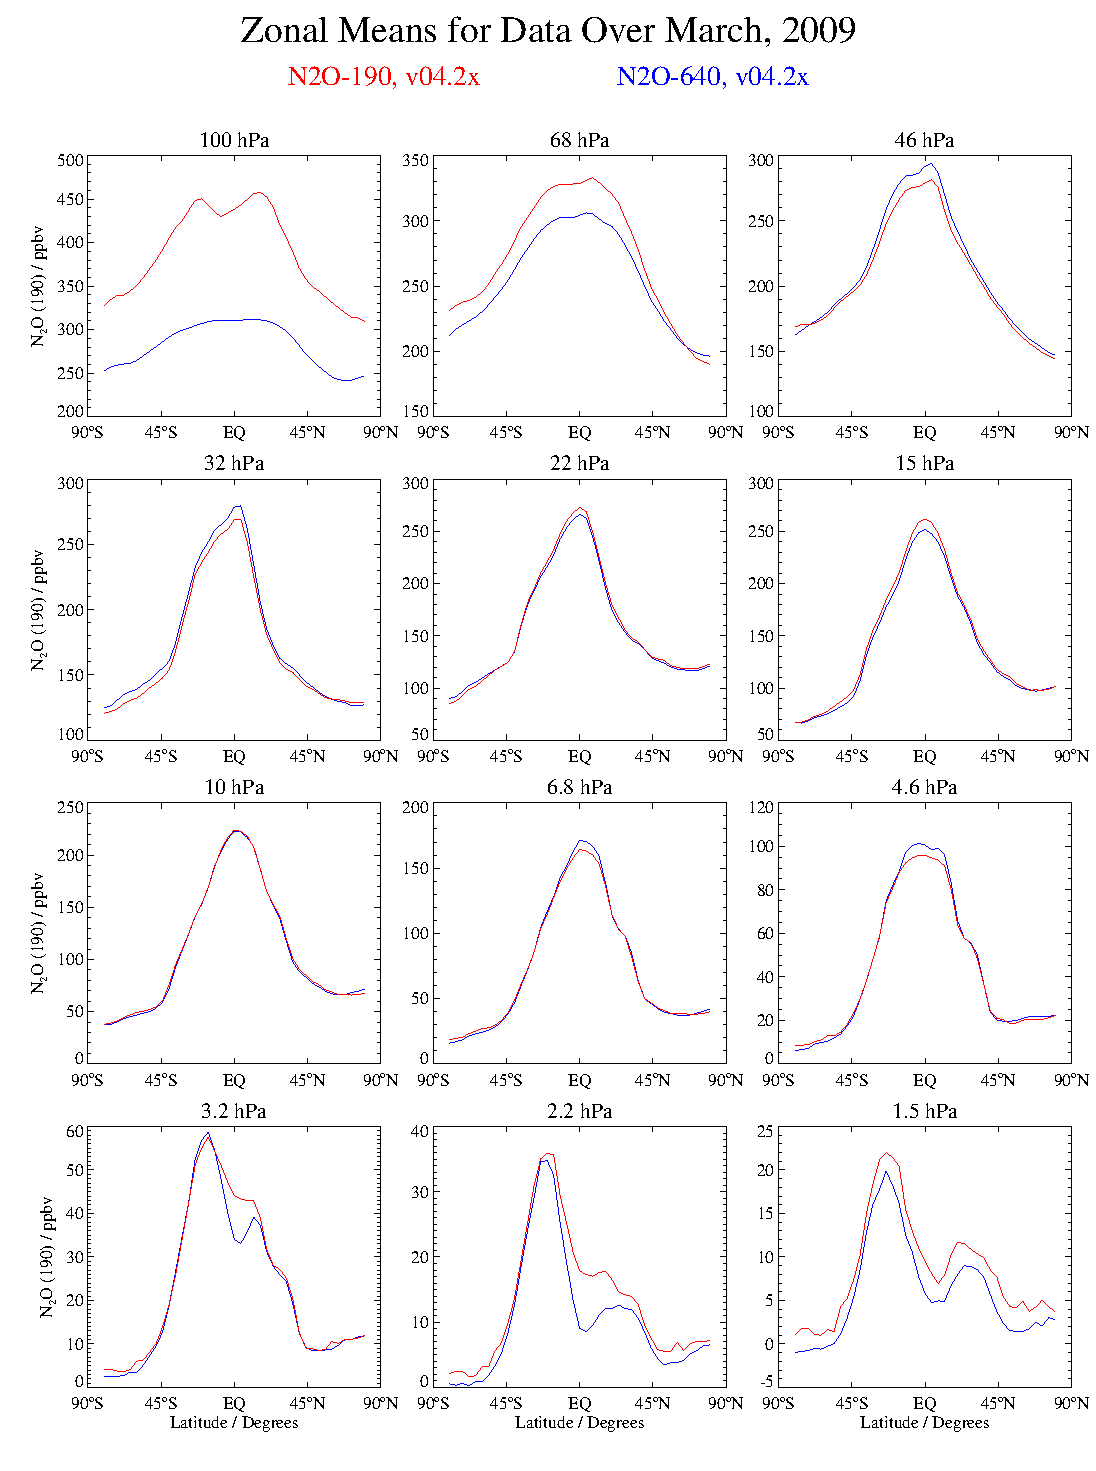
\includegraphics[width=\linewidth]{figures/InspectZM_2009m03_N2O-190-v04-2x_N2O-640-v04-2x_userHeightRange}
\caption{MLS \thisv \texttt{N2O-190} and \texttt{N2O-640} comparison for
  March 2009}
\label{fig:N2O190640Comparison}
\end{figure}

Other significant differences between the \thisv \texttt{N2O-190} and
\texttt{N2O-640} data such as the resolution, precision, recommended pressure levels, 
quality and convergence criteria are noted below.

The secondary \thisv N\cs2O 640-GHz product is available for the period
from launch until June 6, 2013 and stored in the \texttt{L2GP-DGG} files
in the \texttt{N2O-640} swath.  Details of the retrieval method and
validation results are presented in \citep{LambertEtal:2007}.

\subsection{Resolution}

\onestandardavk{N2O-190}{190\,GHz N\cs2O}

\onestandardavk{N2O-640}{640\,GHz N\cs2O}

The spatial resolution reported by the averaging kernel matrices is
shown in Figures~\ref{fig:AvkN2O-190} for the 190\,GHz measurements
and~\ref{fig:AvkN2O-640} for the 640\,GHz measurements (available in the
\texttt{L2GP-DGG} files for data prior to June~6, 2013).  For
\texttt{N2O-190}, the vertical resolution is 4\,--\,8\,km and the
horizontal along-track resolution is 300\,--\,600\,km.  For
\texttt{N2O-640}, the vertical resolution is 4\,--\,6\,km and the
horizontal along-track resolution is 300\,--\,600\,km over most of the
useful range of the retrievals.

The horizontal cross-track resolution is set by the 7\,km width of the
MLS 190-GHz field-of-view for all pressures. Note that the higher
frequency MLS 640-GHz measurements have a narrower 3\,km field-of-view.
The longitudinal separation of the MLS measurements is
10\degsym--\,20\degsym\ over middle and lower latitudes, with much finer
sampling in polar regions.

\subsection{Precision}

Precision as defined here is the $1\sigma$ uncertainty in the retrieved
value calculated by the Level~2 algorithms and has been validated
against the scatter about the mean of coincident ascending/descending
MLS profile differences.  The estimated precision on a single retrieved
profile given in Tables~\ref{tab:N2OSummary} and~\ref{tab:N2O640Summary}
varies with height from \texttildelow15\,--\,20\,ppbv for \texttt{N2O-190} and
\texttildelow12\,--\,25\,ppbv for \texttt{N2O-640}.

The N\cs2O values at the 147\,hPa pressure level have a large a priori
influence and practically all precisions are flagged negative at this
level.

\subsection{Accuracy}

The accuracy values given in Table~\ref{tab:N2O640Summary} were obtained
for both v4 N\cs2O products using the same detailed analyses presented
for MLS \texttt{N2O-640} v2.2 data in \citet{LambertEtal:2007} to quantify
the systematic uncertainties associated with the MLS instrument
calibration, spectroscopic uncertainty and approximations in the
retrieval formulation and implementation.

\subsection{Data screening}
\label{sec:N2OScreening}
\begin{description}
\item[Pressure range (\texttt{N2O-190}):] \screeningrule{68\,--\,0.46\,hPa}
\item[Pressure range (\texttt{N2O-640}):] \screeningrule{100\,--\,0.46\,hPa}
\standardrangestatement\ In the upper stratosphere and lower
  mesosphere \thisv N\cs2O requires significant averaging for useful
  signals, but see the note under ``Artifacts'' for issues at pressures below
  0.1\,hPa.

\standardprecisionrule
\evenstatusrule

\item[Quality (\texttt{N2O-190}):] \qualityrule{1.0} Note that this is a
  change from the threshold originally suggested for \thisv.  See the
  discussion of this topic below.

\item[Convergence (\texttt{N2O-190}):] \convergencerule{2.0}
  A fraction of the \texttt{N2O-190} data (typically less than 0.5\%) at this level
  will be discarded via this screening.

\item[Quality (\texttt{N2O-640}):] \qualityrule{1.4}
  A small fraction of \texttt{N2O-640} profiles (typically less than 0.5\%) will
  be discarded via this screening.

\item[Convergence (\texttt{N2O-640}):] \convergencerule{1.01}
  A fraction of the \texttt{N2O-640} data (typically less than 0.5\%) at this level
  will be discarded via this screening.

\item[Clouds:] \screeningrule{Clouds have little impact on the N\cs2O products at the recommended pressure levels. 
Ignore status bit 16 (high cloud) or bit 32 (low cloud) indicating the presence of clouds. See
artifacts for more details.}

\end{description}

\subsubsection{Updated \texttt{Quality} screening recommendation}
A byproduct of the aging in MLS that gives rise to the drift in the
water vapor product (see section~\ref{sec:H2ODrift}) and 190-GHz N\cs2O
(see below) is that the \texttt{Quality} metric for the 190-GHz N\cs2O
product exhibits a decreasing trend (most notable in the years following
\texttildelow2009).  This decrease is not correlated with any actual
decline in the accuracy of the MLS N\cs2O product, which appears largely
unchanged (drift issues aside).  However, application of the previously
recommended 1.3 \texttt{Quality} threshold leads to rejection of an
unreasonably large fraction of the N\cs2O profiles in the more recent
years of the Aura mission, particularly during southern winter.  The
revised 1.0 \texttt{Quality} threshold restores these profiles without
erroneously identifying any obviously poor profiles as acceptable.

\subsection{Artifacts}
\label{sec:N2ODrift}

In addition to the large bias of the 190-GHz N\cs2O at 100\,hPa (not
removed by screening), there are occasional outliers at the highest
presure levels in \texttt{N2O-190} and \texttt{N2O-640} products. 
Very thick clouds in the tropics produce a low rate of artifacts in the \thisv N\cs2O
products since improvements in the handling of radiances affected by
clouds have reduced the frequency of outliers compared to previous
versions. The cloud bits of the \texttt{Status} field are too blunt a
tool to identify these rare cases, needlessly discarding reasonable data.
Screening using the convergence
and quality fields (see above) is recommended to remove the majority of
these data points. 

The retrieval restricts N\cs2O values to be greater than
$-40\,\text{ppbv}$ (approximately three times the retrieval noise level
in the recommended pressure range) in order to prevent problems in the
minimization search process.  The low bound is applied at all levels,
but it is only evident in the data for pressures less than 0.1\,hPa,
where the vertical smoothing is relaxed and the retrieval noise becomes
comparable to the magnitude of the low bound value.  Accordingly,
statistical averaging of the data (zonal means or longer time periods)
cannot be applied successfully for pressures at and less than 0.1\,hPa
as the $-40\,\text{ppbv}$ hard limit introduces a positive bias in any
average.

A long-term trend of about $-0.5\%$ per year has been observed in the
MLS \texttt{N2O-190} data product, through analysis of the mean values
in the equatorial lower stratosphere in the years following 2009.  Since
the long term secular increase in tropospheric N\cs2O observed by
ground-based instruments is about $+0.25\%/\text{year}$, the anomalous
MLS \texttt{N2O-190} drift giving rise to the observed \texttt{N2O-190}
trend is probably around $-0.75\%/\text{year}$. The cause of this small
but statistically significant drift is under investigation.

\subsection{Review of comparisons between MLS N\cs2O  versions and other datasets}

Average values for \thisv 190-GHz N\cs2O are up to 10\% smaller than in v2.2 for the
100 and 68\,hPa pressure levels, and within a few percent for pressures greater than 46\,hPa 
(see Figure~\ref{fig:N2O190Comparison}). Differences between \thisv 190-GHz N\cs2O and
v3.3 are less than a few percent at all levels.

\begin{figure}
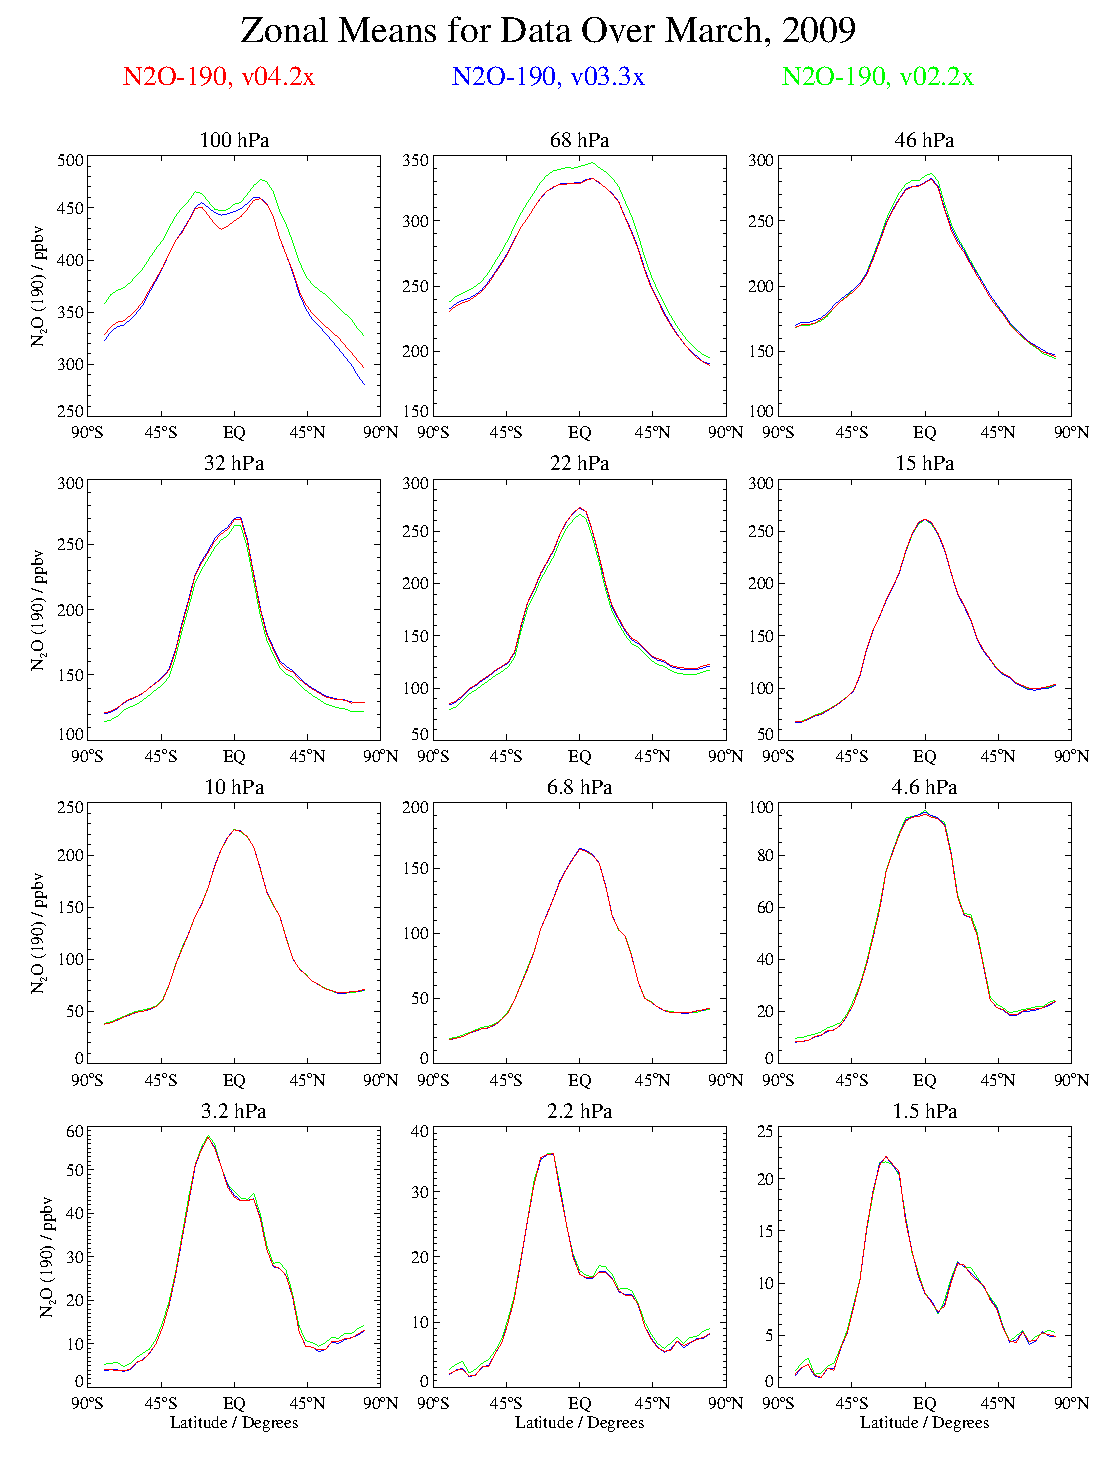
\includegraphics[width=\linewidth]{figures/InspectZM_2009m03_N2O-190-v04-2x_N2O-190-v03-3x_N2O-190-v02-2x_userHeightRange}
 \caption{MLS v4.2 190-GHz N\cs2O compared to v2.2 and v3.3 for March 2009}
\label{fig:N2O190Comparison}
\end{figure}

Average values for \thisv 640-GHz N\cs2O are 20\% larger than in v2.2
for the 100\,hPa pressure level, up to 10\% smaller at the
46\,--\,32\,hPa levels, and within 5\% for pressures greater than
22\,hPa (see Figure~\ref{fig:N2O640Comparison}). Differences between
\thisv 640-GHz N\cs2O and v3.3 are less than a few percent at all
levels. Unlike the \texttt{N2O-190} product, the \texttt{N2O-640}
product is recommended for scientific use at 100\,hPa.

Apart from the differences noted above, the MLS \thisv 640 GHz N\cs2O is
similar to the MLS v2.2 product described and validated in
\citet{LambertEtal:2007}.  Comparisons of v2.2 640 GHz N\cs2O with
coincident measuremements by ACE-FTS, Odin/SMR, and Envisat/MIPAS and
balloon borne observations are shown in \citet{LambertEtal:2007}.  A
revised validation paper for N\cs2O is not planned in the near future
and users are encouraged to read \citet{LambertEtal:2007} for more
information.

\begin{figure}
  \includegraphics[width=\linewidth]{figures/InspectZM_2009m03_N2O-640-v04-2x_N2O-640-v03-3x_N2O-640-v02-2x_userHeightRange}
 \caption{MLS v4.2 640 GHz N\cs2O compared to v2.2 and v3.3 for March 2009}
\label{fig:N2O640Comparison}
\end{figure}

\subsection{Desired improvements for future data version(s)}

Retrievals of N\cs2O to pressures greater than 100\,hPa \emph{may} be
possible in later versions from the 190-GHz observations.

\begin{table}[b]
  \caption{Summary of MLS \thisv N\cs2O (\texttt{N2O-190}) product.}\vspace{0.5ex}
\label{tab:N2OSummary}
\begin{minipage}{\linewidth}
\centering\begin{tabular}{ccccccl}
\toprule
\parbox[m]{15mm}{\centering\textbf{Region}} &
\parbox[m]{24mm}{\centering\textbf{Resolution\\ Vert. $\times$ Horiz.}} &
\multicolumn{2}{c}{\parbox[m]{18mm}{\centering\textbf{Precision\footnote{Precision on individual profiles}}}} &
\multicolumn{2}{c}{\parbox[m]{15mm}{\centering\textbf{Accuracy}}} &
\textbf{Comments} \\
\textbf{hPa} & \textbf{km} &  \textbf{ppbv} & \textbf{\%} & \textbf{ppbv} & \textbf{\%} & \\
\midrule
$\leq$0.33   & ---                 & ---   & ---       & --- & --- & Unsuitable for scientific use \\   
0.46         &  11.0 $\times$  655 &   15  & $>$100 &  2  & $>$100 & \\ 
0.68         &   9.7 $\times$  540 &   17  & $>$100 &  2  & 89 & \\ 
1.0          &   8.6 $\times$  440 &   18  & $>$100 &  2  & 50 & \\ 
2.2          &   7.3 $\times$  340 &   19  &   64   &  4  & 36 & \\ 
4.6          &   6.5 $\times$  285 &   17  &   23   &  5  & 11 & \\ 
10           &   6.0 $\times$  265 &   16  &   12   &  7  &  7 & \\ 
22           &   5.6 $\times$  305 &   15  &    9   & 10  &  6 & \\ 
46           &   4.9 $\times$  385 &   14  &    7   & 30  & 10 & \\ 
68           &   5.4 $\times$  420 &   16  &    6   & 55  & 22 & \\
100          &   3.8 $\times$  500 &   20  &    7   &124  & 44 & Consult with MLS science team\\ 
147          & ---                 & ---   & ---    & --- & ---& Unsuitable for scientific use \\   
$\geq$215    & ---                 & ---   & ---    & --- & ---& Not retrieved \\\bottomrule
\end{tabular}
\end{minipage}
\end{table}

\begin{table}[b]
  \caption{Summary of MLS \thisv N\cs2O (\texttt{N2O-640}) product.}\vspace{0.5ex}
\label{tab:N2O640Summary}
\begin{minipage}{\linewidth}
\centering\begin{tabular}{ccccccl}
\toprule
\parbox[m]{15mm}{\centering\textbf{Region}} &
\parbox[m]{24mm}{\centering\textbf{Resolution\\ Vert. $\times$ Horiz.}} &
\multicolumn{2}{c}{\parbox[m]{18mm}{\centering\textbf{Precision\footnote{Precision on individual profiles}}}} &
\multicolumn{2}{c}{\parbox[m]{15mm}{\centering\textbf{Accuracy}}} &
\textbf{Comments} \\
\textbf{hPa} & \textbf{km} &  \textbf{ppbv} & \textbf{\%} & \textbf{ppbv} & \textbf{\%} & \\
\midrule
$\leq$0.33   & ---                 & ---   & ---       & --- & --- & Unsuitable for scientific use \\   
0.46         &   8.9 $\times$  530 &   12  &  $>$100   &  1 & 88  & \\     
0.68         &   7.4 $\times$  430 &   13  &  $>$100   &  2 & 89  & \\     
1.0          &   6.2 $\times$  345 &   14  &  $>$100   &  2 & 50  & \\   
2.2          &   4.8 $\times$  300 &   15  &   49      &  3 & 27  & \\   
4.6          &   4.1 $\times$  295 &   14  &   18      &  6 & 14  & \\          
10           &   3.9 $\times$  360 &   13  &   10      & 12 & 11  & \\          
22           &   4.2 $\times$  410 &   14  &    8      & 22 & 14  & \\          
46           &   4.4 $\times$  495 &   16  &    7      & 40 & 19  & \\          
68           &   5.5 $\times$  555 &   20  &    8      & 70 & 28  & \\          
100          &   5.2 $\times$  610 &   25  &    9      & 51 & 18  & \\          
147          & ---                 & ---   & ---       & --- & --- & Unsuitable for scientific use \\   
$\geq$215    & ---                 & ---   & ---       & --- & --- & Not retrieved \\
\bottomrule
\end{tabular}
\end{minipage}
\end{table}

%%% Local Variables:  
%%% mode: latex 
%%% TeX-master: "v5-x-report" 
%%% End:  


\speciestitle{Ozone}{O\cs3}{O3}%
\begin{description}
\item[Useful range:] 261\,--\,0.02\,hPa  
\item[Contact:] Lucien Froidevaux (stratosphere/mesosphere), 
  \email{Lucien.Froidevaux@jpl.nasa.gov} \\ 
  Michael Schwartz (upper troposphere), 
  \email{Michael.J.Schwartz@jpl.nasa.gov} 
\end{description} 
\label{sec:StandardO3} 
 
\subsection*{Introduction} 
 
The \thisv standard O\cs3 product is taken from the 240-GHz retrieval,
which provides the highest sensitivity down into the upper troposphere,
as well as in the mesosphere.  Table~\ref{tab:O3Summary} summarizes the
typical resolution, precision, and systematic uncertainty estimates as a
function of pressure.  Papers describing detailed validation of the MLS
v2.2 product and comparisons with other data sets were published in a
special Aura validation issue of the {\it Journal of Geophysical
  Research}, see \citep{FroidevauxEtal08O3,JiangYEtal07,LiveseyEtal08}.  In
the stratosphere and above, \thisv ozone profiles are very similar to the
v2.2 profiles, so the stratospheric results from the above references
will generally hold for the \thisv product.  Initial documentation of
changes, improvements, and issues with \thisv data are discussed here,
including data screening criteria (which are now somewhat more complex
than in v2.2 data).  The morphology of the (zonal mean) \thisv ozone data
appears to be more reliable (realistic) for the largest pressure values
where ozone is retrieved in the upper troposphere, notably at 316\,hPa
and also at 261\,hPa (a new level for \thisv). The 316\,hPa ozone
retrievals will, however, require further validation before we can
recommend this pressure surface for scientific use.
 
There are 2 separate stratospheric ozone columns (typically in very good
agreement) in the \texttt{L2GP-O3} files, with swath names
%
`\verb*+O3 column-MLS+'
%
and
%
`\verb*+O3 column-GEOS5+',
%
corresponding to the use of tropopause pressures (WMO definition)
determined from MLS or GEOS-5 temperatures, respectively.  Data users
can also provide their own calculations of column ozone values (with
better screening), based on the MLS ozone profiles, given that poorly
defined tropopause values can lead to relatively large scatter at
certain places (and times) for ozone column results.
 
\subsection*{Comparison of \thisv with v2.2} 
 
Between 316\,hPa and 1\,hPa, \thisv ozone profiles are retrieved on 12
surfaces per decade, a grid twice as fine as the 6-level-per-decade grid
used in v2.2. This finer grid makes possible some improvement in
vertical resolution in the UTLS, with retrieved precisions similar to
(or slightly larger than) the v2.2 values, but at the cost of poorer
horizontal resolution (see Table\ref{tab:O3Summary}.)  For pressures
less than 1\,hPa, the retrieval grid has not changed from the v2.2 grid;
it becomes coarser, with 6 surfaces per decade change in pressure
between 1 and 0.1\,hPa, and 3 surfaces per decade change in pressure
from 0.1\,hPa to 0.01\,hPa.  Other changes in the retrievals for the
240-GHz phase (affecting CO and HNO\cs3 as well as ozone) include the
manner in which the spectral baseline is modeled.  The \thisv retrieval
fits a relative-humidity-like, frequency squared extinction baseline at
the lowest retrieval levels, rather than a spectrally flat extinction
profile, as used in v2.2.  This modification reduces ozone biases in the
upper troposphere in moist clear air (or thin cloud) conditions, but
gives a poorer fit to the impacts of thick clouds (scattering from ice
particles in convective cores).  Cloud effects lead to more scatter and
vertically-oscillating profiles in \thisv, for the most part in the
tropics, and methods to screen out cloud-impacted profiles are discussed
below.  Also, there have been relatively minor spectroscopic changes for
these \thisv ozone retrievals: the line mixing parameters are now taken
from the recent (unpublished) work of {\it DeLucia et al.}.
 
\begin{figure} 
\centering\dontincludegraphics[angle=90,width=\linewidth]%
{figures/InspectZMContour_O3--v2-2_O3--v3-3_2006m11_LatPress-All-NaN-Allheights} 
\caption{Zonal averages for stratospheric and mesospheric MLS ozone
  profiles during November, 2006, showing the MLS v2.2 ozone mixing
  ratio contours (top left panel), the \thisv contours (top right panel),
  and their differences in ppmv (\thisv minus v2.2, bottom left panel) and
  percent (\thisv minus v2.2 versus v2.2, bottom right panel). }
\label{fig:MLSv2v3O3ContourStrat} 
\end{figure} 
 
\begin{figure} 
\centering\dontincludegraphics[angle=90,width=\linewidth]%
{figures/InspectZMContour_O3--v2-2_O3--v3-3_2006m11_LatPress-All-NaN-UT} 
\caption{Zonal averages for UTLS MLS ozone profiles during November,
  2006, showing the MLS v2.2 ozone mixing ratio contours (top left
  panel), the \thisv contours (top right panel), and their differences in
  ppmv (\thisv minus v2.2, bottom left panel) and percent (\thisv minus v2.2
  versus v2.2, bottom right panel). }
\label{fig:MLSv2v3O3ContourUTLS} 
\end{figure} 
 
Figures \ref{fig:MLSv2v3O3ContourStrat} and
\ref{fig:MLSv2v3O3ContourUTLS} show zonally averaged fields for the
(full) month of November, 2006, with only the properly screened profiles
from v2.2 and \thisv being used; mean differences (ppmv and percent) are
also shown.  The averages for stratospheric (and lower mesospheric)
ozone have typically not changed by more than 0.1\,ppmv,or 1 to 2\%; see
Figure \ref{fig:MLSv2v3O3ContourStrat}.  At low latitudes, zonal-mean
\thisv tends to be \texttildelow10\,ppbv larger than v2.2 from 215\,hPa to
100\,hPa, while at higher latitudes, the v2.2/\thisv relationship tends
to switch signs, with \thisv higher than v2.2 at 316\,hPa and 147\,hPa,
and lower at 215\,hPa and 100\,hPa (see Figure
\ref{fig:MLSv2v3O3ContourUTLS}).  Also, we note that the version 3.3
mean tropical profiles in the UTLS can exhibit significant systematic
vertical oscillations, mostly apparent during certain months (see the
`Artifacts' section below).

\paragraph*{Ozone Columns:} Changes in the MLS stratospheric ozone
columns (or in columns down to pressures between 100 and 316\,hPa) for
\thisv are quite small; typical daily zonal averages are within one
percent, and often within one DU.  There is no significant systematic
offset (offsets can change slightly between pressure levels and versus
latitude, including changes in sign).  The most significant difference
is the change in scatter, as observed for example in standard deviations
about zonal averages (with \thisv scatter often lower than in v2.2 by
several DU); this is largely a result of (and at the expense of) changes
in the horizontal smoothing, and poorer horizontal resolution for \thisv
data (see below).

 
\subsection*{Resolution} 
%\onestandardavk{O3_HR}{O\cs3} 
 
\begin{figure} 
\centering\dontincludegraphics[width=0.5\linewidth]{figures/avk-v3-3-O3_HR-35N} 
\caption{Typical two-dimensional (vertical and horizontal along-track)
  averaging kernels for the MLS \thisv O\cs3 at the equator; variation in
  the averaging kernels is sufficiently small that these are
  representative of typical profiles.  Colored lines show the averaging
  kernels as a function of MLS retrieval level, indicating the region of
  the atmosphere from which information is contributing to the
  measurements on the individual retrieval surfaces, which are denoted
  by plus signs in corresponding colors.  The dashed black line
  indicates the resolution, determined from the full width at half
  maximum (FWHM) of the averaging kernels, approximately scaled into
  kilometers (top axes).  (Upper) Vertical averaging kernels (integrated
  in the horizontal dimension for five along-track profiles) and
  resolution.  The solid black line shows the integrated area under each
  kernel (horizontally and vertically); values near unity imply that the
  majority of information for that MLS data point has come from the
  measurements, whereas lower values imply substantial contributions
  from a priori information.  (Lower) Horizontal averaging kernels
  (integrated in the vertical dimension) and resolution.  The averaging
  kernels are scaled such that a unit change is equivalent to one decade
  in pressure.}
\label{fig:avkO3Strat} 
\end{figure} 
 
\begin{figure} 
  \centering\dontincludegraphics[width=0.5\linewidth]{figures/avk-v3-3-O3_HR-35N-UTLS}
\caption{As for \protect{\ref{fig:avkO3Strat}} but zooming in on the
    upper troposphere and lower stratosphere region.}
\label{fig:avkO3UTLS} 
\end{figure} 
 
Vertical and horizontal smoothing constraints were changed for \thisv data
in an attempt to capitalize upon the higher vertical resolution offered
by the finer grid, while minimizing the vertical oscillations invited by
the additional vertical degrees of freedom.  Based on the width of the
averaging kernels shown in Figures~\ref{fig:avkO3Strat}
and~\ref{fig:avkO3UTLS}, the vertical resolution for the standard O\cs3
product is \texttildelow2.5\,km in the uppermost troposphere and stratosphere,
but degrades to 4 to 6\,km in the upper mesosphere and to \texttildelow3\,km at
316\,hPa. At best, lower stratospheric resolution can be about 2.3\,km,
which is an improvement over v2.2 data (but not by a factor of two --
the best resolution offered by the new 12-per-decade grid).  The
along-track resolution in the stratosphere has changed from \texttildelow
200\,km in v2.2 to 300 to 450\,km in \thisv, depending on altitude (the
upper stratosphere shows poorer resolution). In the mesosphere, this
along-track resolution varies between about 300 and 700\,km. In the
upper troposphere, the along-track resolution degrades from
\texttildelow300\,km at 120\,hPa to \texttildelow450\,km at 261\,hPa.  Typical
resolution values are provided in the summary Table~\ref{tab:O3Summary}.
The cross-track resolution is set by the 6\,km width of the MLS 240\,GHz
field of view.  The longitudinal separation of MLS measurements, set by
the Aura orbit, is 10\degsym--\,20\degsym\ over middle and lower
latitudes, with much finer sampling in polar regions.
 
\subsection*{Precision} 
 
The horizontal smoothing changes in \thisv, coupled with the finer
vertical retrieval grid, have led to some changes in estimated precision
(keeping in mind, however, the poorer \thisv horizontal resolution).  In
the upper stratosphere, the precisions are improved (smaller values) by
about 30\% in the \thisv data, although there is no need to quote
substantially different values than the (rounded off) values that are
given in Table~\ref{tab:O3Summary}.  In the UTLS, the Level 2 ozone
precision (uncertainty) values have worsened slightly (by \texttildelow20 to
30\%) from v2.2 to \thisv.  As found previously for v2.2 data, the Level~2
precision values are often slightly lower than the observed scatter in
the data, evaluated in a narrow latitude band centered around the
equator where atmospheric variability is expected to be small, or
obtained from a comparison between ascending and descending coincident
MLS profiles.
 
Negative precision values for ozone occur essentially for every data
point at pressures smaller than 0.01\,hPa, indicating increasing
influence from the \emph{a priori}, although some MLS information exists
(e.g., regarding average day/night differences) into the uppermost
mesosphere and lower thermosphere.  Generally, however, we recommend
that scientific studies be restricted to pressures of 0.02\,hPa or
larger.
 
\paragraph*{Column values:} As for the v2.2 retrievals, the estimated
precisions for the \thisv MLS column ozone abundances down to pressures of
100 to 215\,hPa are 2\% or less.  The typical empirical precision in the
columns based on (1-$\sigma$) variability in the tropics is 2 to 3\%.
However, see the comments above regarding the somewhat poorer
along-track (horizontal) resolution for \thisv data.
 
\subsection*{Accuracy} 
 
The accuracy estimates shown in Table~\ref{tab:O3Summary} are from an
analysis which propagated estimated systematic errors in MLS
calibration, spectroscopy, etc., through the v2.2 measurement system.
Results using the \thisv algorithms are not expected to differ
significantly.  The values shown here are intended to represent
2$\sigma$ estimates of accuracy.  Overall, we see no evidence, based on
a number of (published) comparisons with well established data sets,
that significant disagreements (outside the combined accuracy estimates)
or MLS-related issues exist for the MLS ozone product.  For more
details, see the MLS validation papers by \citet{FroidevauxEtal08O3},
\citet{JiangYEtal07}.  and \citet{LiveseyEtal08}, as well as references
therein; some more recent references relevant to MLS ozone and ozone
columns are available on the MLS website under `Publications'.  Future
validation studies using \thisv data will focus on longer-term changes and
on the UTLS region.
 
\paragraph*{Column values:} Sensitivity tests using systematic changes
in various parameters that could affect the accuracy of the MLS
retrievals lead to possible biases (2-$\sigma$ estimates) of about 4\%,
as an estimated accuracy for the MLS column values (from integrated MLS
ozone profiles down to 100, 147, and 215\,hPa).  See also the (v2.2)
validation papers (and subsequent ozone-related publications, e.g.,
available from the MLS website) for results on column ozone comparisons
versus satellite, sonde, and lidar data.
 
\subsection*{Data screening} 
\begin{description} 
 
\item[Pressure range:] \screeningrule{261\,--\,0.02\,hPa.}
  \standardrangestatement 
  \standardprecisionrule
  \evenstatusrule
\item[Quality:] \qualityrule{0.6}
\item[Convergence:] \convergencerule{1.18}
\item[Clouds:] \screeningrule{Scattering from thick clouds can lead to oscillatory
    values for O\cs3 in the UT/LS, see below for screening rules.}

  Most of the affected profiles are removed by the \texttt{Quality},
  \texttt{Convergence}, and outlier screening methods, as described below, 
  specifically for the \thisv data.
\item[`Outlier' Screening:] The \thisv ozone product has more tropical
  outliers than the v2.2 data in the lower stratosphere (mainly a few to
  a few tens of positive outliers at 68\,hPa on a typical day) and in
  the upper troposphere, where both negative or positive spikes can
  dominate, depending on the pressure level.  As for CO, these often
  appear to be related to thick clouds, and large values of ice water
  content (IWC) in the vicinity of the affected profiles.
  
  We have found that using explicit thresholds for negative ozone spikes
  at pressures larger than the 46\,hPa MLS pressure level can effectively
  screen out most of the outliers, including most of the \emph{positive}
  outliers in the UTLS.  The recommended screening method for \thisv ozone
  should therefore also include a test for significantly negative values
  for the MLS pressure range from 56 to 261\,hPa (inclusive).  We then
  recommend rejection of \emph{all values in this range} when a
  (negative) mixing ratio less than $-$0.15\,ppmv is encountered (for any
  level in this range); in addition, any value at 316\,hPa less than
  $-$0.30\,ppmv should also lead one to discard the applicable UTLS values.
  These outlier thresholds are chosen so that large negative values
  outside those thresholds are generally outside the `5 sigma level', in
  relation to typical ozone values and MLS ozone precisions (or scatter)
  in the UTLS; we have also checked that these criteria do not impact
  the screening of high latitude ozone values in any significant way
  (e.g., under ozone hole conditions).

  In summary, one should \emph{reject} profiles with odd \texttt{Status}
  \emph{or} even \texttt{Status} profiles with \texttt{Convergence}
  above the convergence threshold \emph{or} \texttt{Quality} below the
  quality threshold, or with values from 316 to 56\,hPa (inclusive) that
  get eliminated by the negative outlier criteria.  Conversely, one
  should \emph{keep} profile values with even status \emph{and} good
  \texttt{Convergence} \emph{and} good \texttt{Quality} \emph{and}, UTLS
  values in the 316 to 56\,hPa MLS pressure range that do not get
  discarded by the negative outlier criteria.  This methodology does
  remove some profile values that are not in the `outlier' category but
  no method will cleanly remove only the exact number of profiles that
  are suspicious for every day of the MLS mission.  The current
  recommendations typically remove \texttildelow4 to 6 \% of global daily data,
  with some tropical latitudes showing much larger fractional removal
  (e.g., 20 to 30\% in 10\degsym\ bins near the equator).  This
  screening generally maintains sufficient coverage for a near-complete
  daily map (for any given day), even in the UTLS\@.

  Compared to the v2.2 UT data screening recommendations, the screening
  of \thisv UTLS data generally removes slightly more ozone profiles on a
  typical day (although on occasion, slightly less).
 
\begin{figure} 
\centering\dontincludegraphics[angle=90,width=\linewidth]%
{figures/O3-vs-lat-unscreened-2005d343} 
\caption{Example of the MLS ozone mixing ratio distribution versus
  latitude for one day, showing various pressure levels in the UTLS and
  which points are flagged by recommended quality, convergence, and
  outlier criteria (for 2005d343, one of the days showing the most
  outliers). The bottom right panel (for 68\,hPa) also shows (red curve)
  the percentage of points getting screened out in 10\degsym\ latitude
  bins (with the y-axis scaled by a factor of 10) -- close to 30\% of
  points can be thrown out in some bins, on this relatively poor quality
  day.}
\label{fig:O3vsLatUnscreened} 
\end{figure} 
 
\begin{figure} 
\centering\dontincludegraphics[angle=90,width=\linewidth]%
{figures/O3-vs-lat-screened-2005d343} 
\caption{Example of the MLS ozone mixing ratio distribution versus
  latitude for one day, showing various pressure levels in the UTLS and
  which points remain \emph{after} removal of the flagged (colored)
  points shown in the previous Figure.}
\label{fig:O3vsLatScreened} 
\end{figure} 
 
 
Finally, we note that since there is essentially no impact from the
outliers (spikes) in the UTLS (this is also largely a tropical issue) on
the ozone mixing ratios at pressures less than 50\,hPa, it is safe to
ignore the outlier flag in the data screening if a study is only
concerned with pressures smaller than or equal to the 46\,hPa MLS
pressure level; in this case, users can simply apply the
\texttt{Quality} and \texttt{Convergence} (and \texttt{Status}) tests to
obtain a satisfactory data screening method, with fewer profiles removed
(typically less than about 2\% per day, globally) than if the UTLS
screening method were used.
\end{description} 
 
\subsection*{Review of comparisons with other datasets} 
 
O\cs3 comparisons have indicated general agreement at the 5\,--\,10\,\% 
level with stratospheric profiles from a number of comparisons using 
satellite, balloon, aircraft, and ground-based data.  A high MLS v2.2 
bias at 215\,hPa has been obtained in some comparisons versus 
ozonesondes, but this is not observed consistently in other comparisons.  
We have found that latitudinal and temporal changes observed in various 
correlative data sets are well reproduced by the MLS ozone product.  
Future (and ongoing) validation studies using \thisv data will focus more 
on longer-term changes and on the UTLS region, where improvements will 
still be sought, especially in the tropics (see below).
 
\subsection*{Artifacts} 

\begin{figure} 
  \centering\dontincludegraphics[width=\linewidth]%
  {figures/O3_mean_profiles_2006_April_July-v03-v02_25S-25N}
  \caption{Monthly zonal average MLS ozone profiles in the tropical UTLS
    (here, from 316 to 68\,hPa) for 2006 April (left panels) and July
    (right panels), for five 10\degsym \,latitude bins (top to bottom:
    15\degsym\,N--\,25\degsym\,N, 5\degsym\,N--\,15\degsym\,N,
    5\degsym\,S--\,5\degsym\,N, 15\degsym\,S--\,5\degsym\,S,
    25\degsym\,S--\,15\degsym\,S,).  The \thisv profiles are in red, while
    the v2.2 profiles are in blue.}
\label{fig:MLSO3UTtropicalOscillations} 
\end{figure} 

\begin{description}  
\item[Oscillations in tropical UTLS ozone:] The finer resolution and new
  retrieval methodology (and screening) for \thisv allow for improved
  values at 261\,hPa (and to some extent at 316\,hPa, although not a
  recommended level), but some artifacts (oscillations) exist in the
  tropical upper tropospheric profiles.  Indeed, vertical patterns exist
  in monthly means, as shown in Figure
  \ref{fig:MLSO3UTtropicalOscillations} with larger artifacts apparent
  in April (or May) than in July (or August), for example.  Further
  detailed validation and characterization of the MLS tropical UT data
  (in particular) is warranted, in order to more fully understand the
  MLS data limitations for various applications.
\item[Outliers:] Even with the data screening procedures that are
  recommended herein, a few outliers will remain unscreened for some
  days at some pressure levels (with the vast majority of outliers
  occurring at pressures larger than the MLS 46\,hPa level).  Caution is
  advised, not to over-interpret such occasional events.
\item[Columns:] Users of column ozone data above the tropopause from the
  MLS Level 2 files should be aware that the accuracy of these values
  depends on the tropopause pressure accuracy, and that artifacts can
  occur in these calculations, especially at high latitudes (under
  certain temperature gradient conditions).  Users should therefore
  inspect the MLS file values of tropopause pressure if using this
  product (swath) from the MLS ozone files.
\end{description}   
 
\subsection*{Priorities for future data version} 
\begin{itemize}  
\item Reduction of oscillations in UTLS tropical profiles, and retrieval
  improvements in the presence of thick clouds.
\end{itemize}
 
\begin{table} 
\caption{Summary for MLS ozone}\vspace{0.5ex} 
\label{tab:O3Summary} 
\begin{minipage}{\linewidth} 
\centering\begin{tabular}{ccccccl} 
\toprule 
\parbox[m]{15mm}{\centering\textbf{Pressure / hPa}} & 
\parbox[m]{24mm}{\centering\textbf{Resolution\\ Vert. $\times$ Horiz.}} & 
\multicolumn{2}{c}{\parbox[m]{20mm}{\centering\textbf{Precision\footnote{Precision  
        on individual profiles}\\ppmv\hfill\%}}} & 
\multicolumn{2}{c}{\parbox[m]{20mm}{\centering\textbf{Accuracy\footnote{%
        As estimated from systematic uncertainty characterization tests.
        Stratospheric values are expressed in ppmv with a typical
        \emph{equivalent} percentage value quoted.  215\,--\,100\,hPa errors are
        the sum of the ppmv \emph{and percentage} scaling uncertainties quoted.
        Accuracy values, especially for pressures from 100 to 316\,hPa will be
        re-evaluated, but the estimates for v2.2 data are currently used in this
        Table.}% 
      \\ppmv\hfill\%}}}  
& \textbf{Comments} \\ 
\midrule 
$\leq$ 0.01 & ---            & ---  & ---    & ---  & ---  & Unsuitable for scientific use \\   
0.02 & 5.5 $\times$ 200 & 1.4  & 300    & 0.1  &  35  & \\ 
0.05 & 5.5 $\times$ 200 & 0.9  & 150    & 0.2  &  30  & \\ 
0.1  & 4 $\times$ 400 & 0.5  &  60    & 0.2  &  20  & \\ 
0.2  & 3 $\times$ 450 & 0.5  &  40    & 0.1  &   7  & \\ 
0.5  & 3.5 $\times$ 550 & 0.3  &  20    & 0.1  &   5  & \\ 
1    & 3 $\times$ 450 & 0.2  &  7       & 0.2  &   7  & \\ 
2    & 3.5 $\times$ 450 & 0.15  &   3   & 0.2  &   5  & \\ 
5    & 3 $\times$ 450 & 0.15  &   2     & 0.3  &   5  & \\ 
10   & 3 $\times$ 500 & 0.1  &   2      & 0.3  &   5  & \\ 
22   & 2.5 $\times$ 400 & 0.1  &   2    & 0.2  &   5  & \\ 
46   & 2.5 $\times$ 350 & 0.06  &   3   & 0.2  &   8  & \\ 
68   & 2.5 $\times$ 350 & 0.04 & 3--10  & 0.05 & 3--10 & \\ 
100  & 2.5 $\times$ 300 & 0.04 & 20--30 & \multicolumn{2}{c}{$\left[0.05 +5\%\right]$} \\ 
150  & 2.5 $\times$ 400 & 0.03 & 5--100 & \multicolumn{2}{c}{$\left[0.02 +5\%\right]$} \\ 
215  & 3 $\times$ 400   & 0.02 & 5--100 & \multicolumn{2}{c}{$\left[0.02 +20\%\right]$}  \\ 
261  & 3 $\times$ 450   & 0.03 & 5--100 & ---  & ---   &  Requires further evaluation  \\ 
316  & 2.5 $\times$ 500 & 0.05 & ---    & ---  & ---   & Not recommended (until further evaluation) \\ 
1000\,--\,464 & ---     & ---  & ---    & ---  & ---   & Not retrieved \\ 
\bottomrule 
\end{tabular} 
\end{minipage} 
\end{table} 
 
%%% Local Variables:  
%%% mode: latex 
%%% TeX-master: "v4-x-report" 
%%% End:  
 
 
 
 
 
            
 

\speciestitle{Hydroxyl Radical}{OH}{OH}{%
ite\item[Useful range:] 32\,--\,0.0032\,hPa
\item[Contact:] Luis Millan, \email{Luis.F.Millan@jpl.nasa.gov}
  and Shuhui Wang, \email{shw@gps.caltech.edu}}

\subsection{Introduction}

The MLS THz radiometer is dedicated to measuring OH in the 2.5\,THz
spectral region. A description of OH data quality, precision and
systematic errors for an earlier version, v2.2, is given in
\citet{PickettEtal:2006:Validation}. The validation studies are described in
\citet{PickettEtal:2008} and \citet{WangEtal:2008}. While the OH data quality
is generally similar between v2.2 and \prevv, there are significant
improvements in the current version \thisv. In previous versions, OH
data near the mesospheric density peak, \texttildelow0.032 hPa, often
show considerable amount of data flagged with negative precision,
indicating strong influence of \emph{a priori} information, particularly
in the summer hemisphere (or tropics when near the equinox) and
sometimes causes gaps in zonal mean time series. The \thisv software
resolves this issue by fixing the overly tight \texttt{a priori}
constraints. The resulting mesospheric OH data are less noisy and
generally have somewhat larger values than previous versions for the
problematic seasons/latitudes. Another improvement is the smaller bias
at 10\,--\,15\,hPa. Therefore, the day-night correction for bias is only
required for pressure levels at 21 and 32\,hPa. Note that users may
notice more zig-zags in \thisv nighttime mesospheric OH vertical
profiles. This is a side effect of fixing the possible positive bias
introduced by tight lower limits set in previous version retrievals.

The estimated uncertainties, precisions, and resolution for \thisv OH are
summarized in Table~\ref{tab:OHSummary}.

\subsection{Resolution}

Figure~\ref{fig:AvkOH} shows the OH averaging kernel for daytime and
nighttime at 35\degsym N. The reason to separate daytime and nighttime
is that the largest natural variability in OH is diurnal. The vertical
resolution is slightly different between day and night. The nighttime
resolution is sufficient to allow the study of (for example) the
``nighttime OH layer'' around 82\,km.  The vertical width of the
averaging kernel for pressures greater than 0.01\,hPa is\,2.5 km.  The
horizontal width of the averaging kernel is equivalent to a width of
1.5\degsym (165\,km distance) along the orbit.  The changes in vertical
resolution above 0.01\,hPa are due mainly to use of a faster instrument
vertical scan rate for tangent heights above 70\,km.  The horizontal
resolution across track is 2.5\,km. The averaging kernel and resolution
for high and low latitudes are very similar to Figure~\ref{fig:AvkOH}
for most pressure levels.  At the topmost two pressure levels,
0.0046\,hPa and 0.0032\,hPa, the vertical resolution is slightly better
at the equator than at 70\degsym N.

\subsection{Precision}

A typical OH profile and the associated precisions (for both \prevv and
\thisv) are shown in Figure~\ref{fig:OHprofiles}. The profile is shown in
both volume mixing ratio (vmr) and density units. All MLS data are
reported in vmr for consistency with the other retrieved molecules.
However, use of density units (10\cp{6}\,cm\cp{$-$3}) reduces the
apparent steep gradient of OH vertical profile, allowing one to see the
profile with more detail, especially in the stratosphere where most
atmospheric OH is present.  Additionally, at THz frequencies the
collisional line-width is approximately equal to the Doppler width at
1\,hPa. Above 1\,hPa, Doppler broadening is dominant and the peak
intensity of OH spectral absorption is proportional to density, while
below 1\,hPa the peak intensity is proportional to vmr. The daytime OH
density profile shows two peaks at \texttildelow45\,km and \texttildelow75\,km. The
night OH profile exhibits the narrow layer at \texttildelow82 km
\citep{PickettEtal:2006:NightOH}. Precisions are such that an OH zonal
average within a 10\degsym\ latitude bin can be determined with better
than 10\% relative precision with one day of data (\texttildelow100 samples)
over 21\,--\,0.01\,hPa. With 4 days of data, the 10\% precision limits
can be extended to 32\,--\,0.0046\,hPa.

\begin{figure}
\centering\includegraphics[width=0.7\linewidth]{figures/avk-OH}
  \caption{Typical two-dimensional (vertical and horizontal along-track)
    averaging kernels for the MLS \thisv OH data at 35\degsym N for
    daytime (upper) and nighttime (lower); variation in the averaging
    kernels is sufficiently small that these are representative of
    typical profiles. Colored lines show the averaging kernels as a
    function of MLS retrieval level, indicating the region of the
    atmosphere from which information is contributing to the
    measurements on the individual retrieval surfaces, which are denoted
    by plus signs in corresponding colors. The dashed black line
    indicates the resolution, determined from the full width at half
    maximum (FWHM) of the averaging kernels, approximately scaled into
    kilometers (top axes). (Left) Vertical averaging kernels (integrated
    in the horizontal dimension for five along-track profiles) and
    resolution.  The solid black line shows the integrated area under
    each kernel (horizontally and vertically); values near unity imply
    that the majority of information for that MLS data point has come
    from the measurements, whereas lower values imply substantial
    contributions from a priori information. (Right) Horizontal
    averaging kernels (integrated in the vertical dimension) and
    resolution.  The averaging kernels are scaled such that a unit
    change is equivalent to one decade in pressure.}
\label{fig:AvkOH}
\end{figure}

\begin{figure}
\begin{tabular}{@{}l@{}l@{}}
\includegraphics[width=0.5\linewidth]{figures/plot-OHv4-a}&
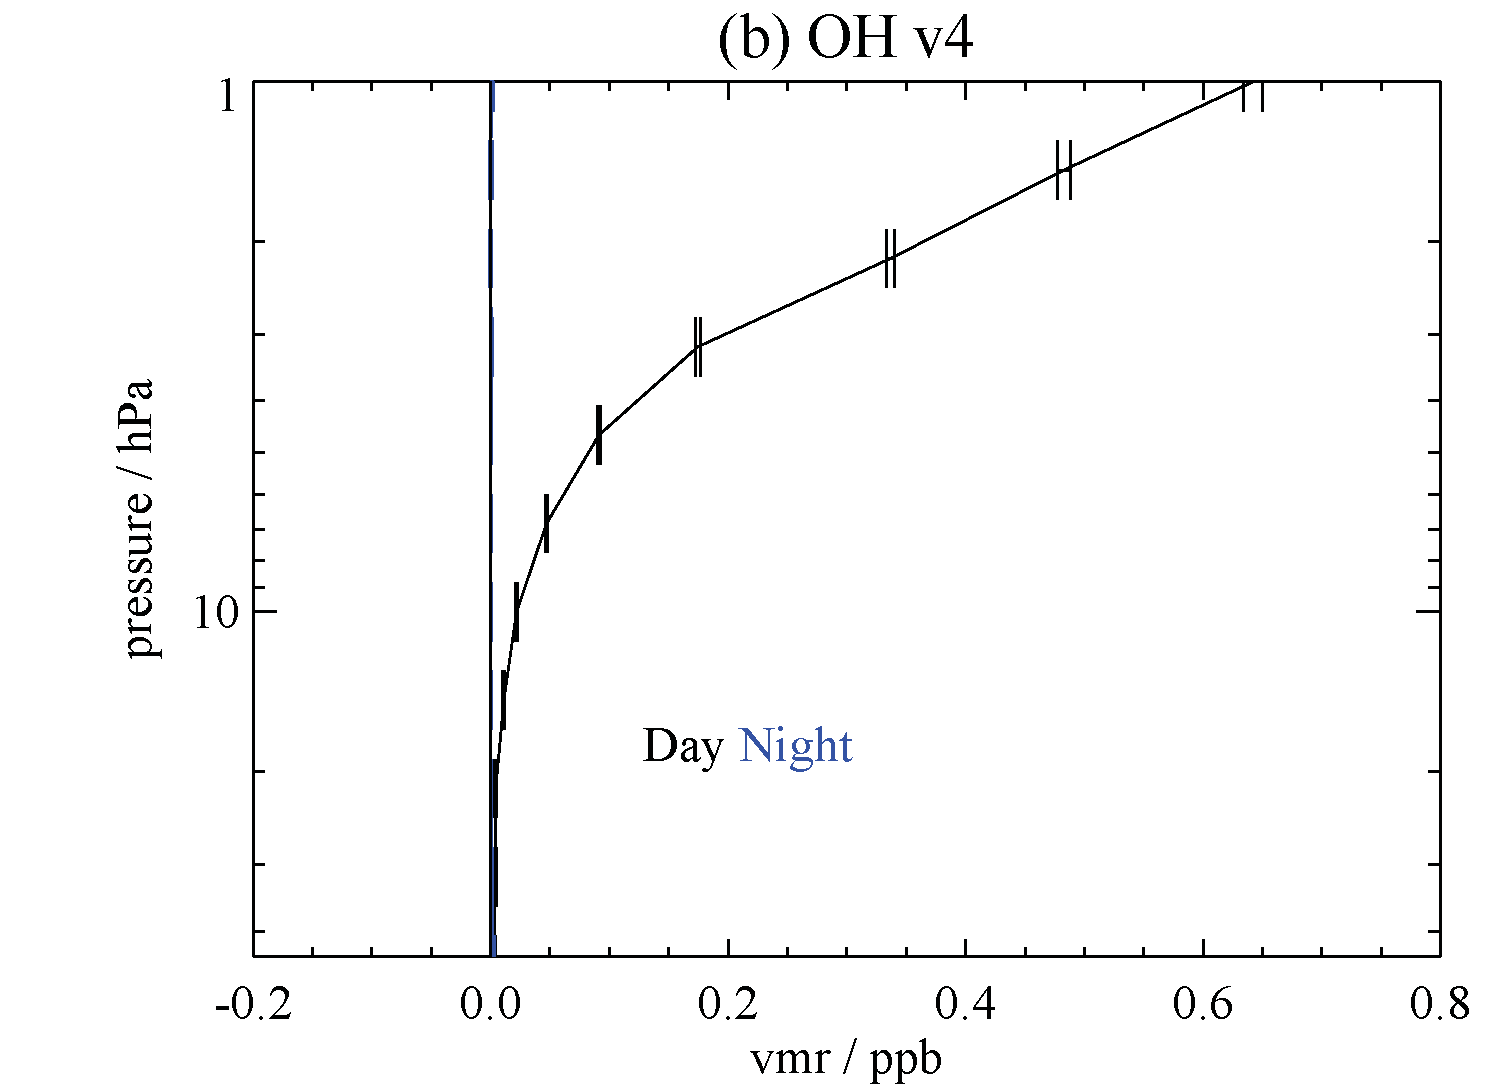
\includegraphics[width=0.5\linewidth]{figures/plot-OHv4-b}\\
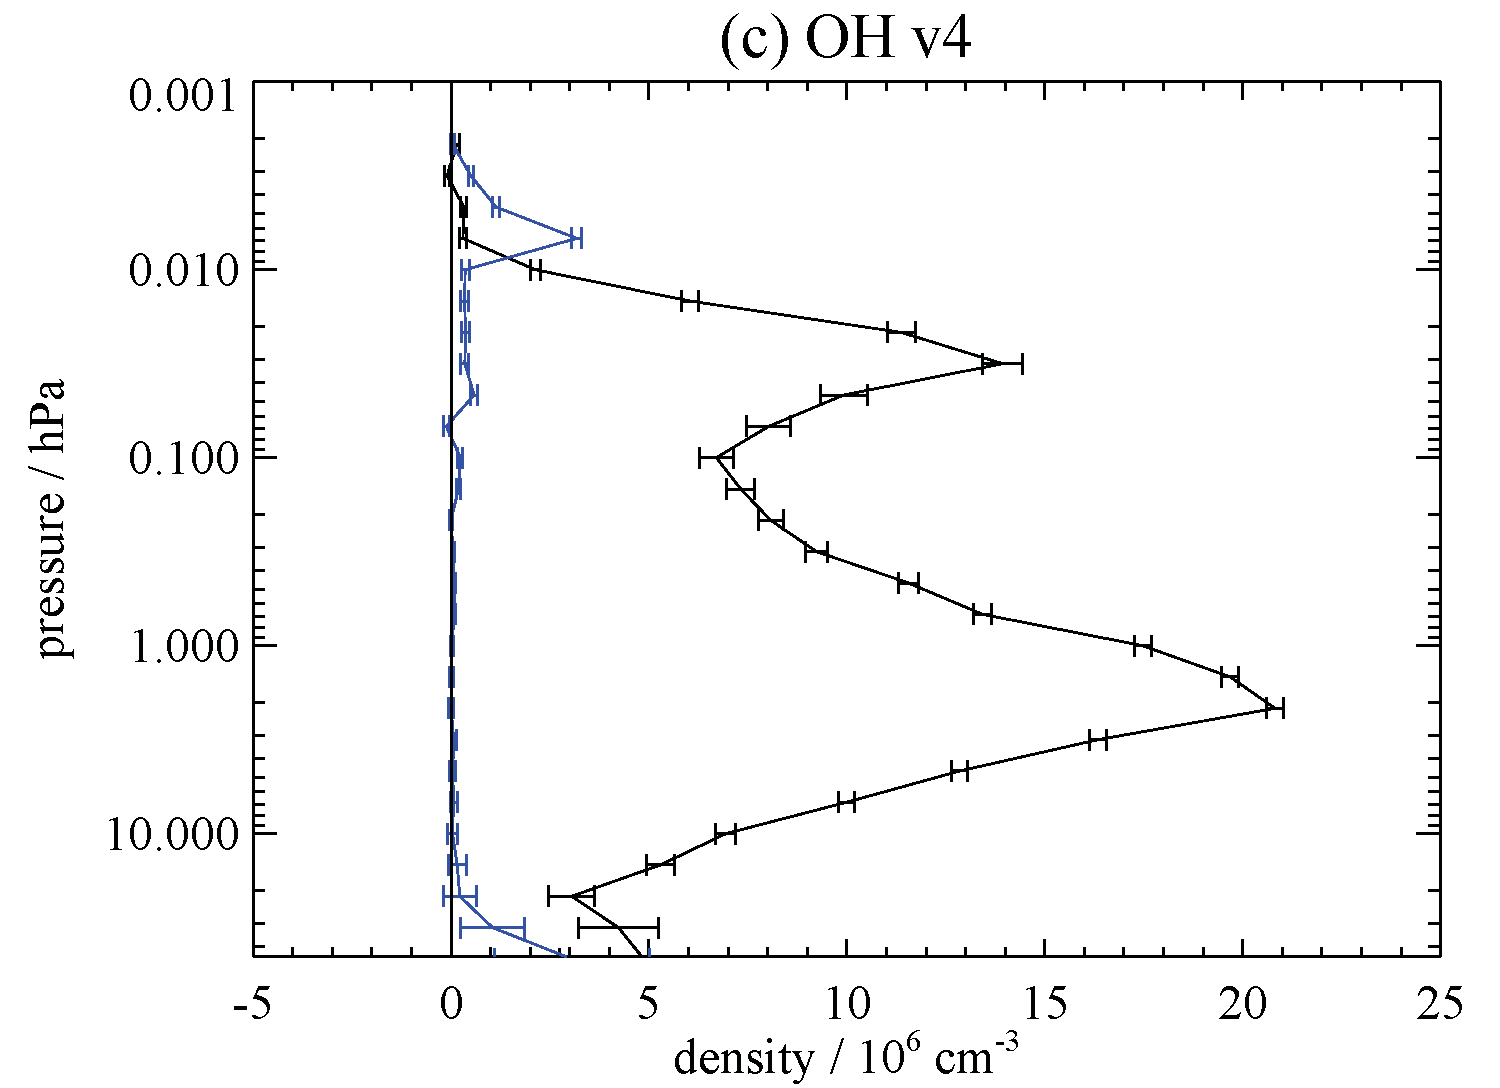
\includegraphics[width=0.5\linewidth]{figures/plot-OHv4-c}&
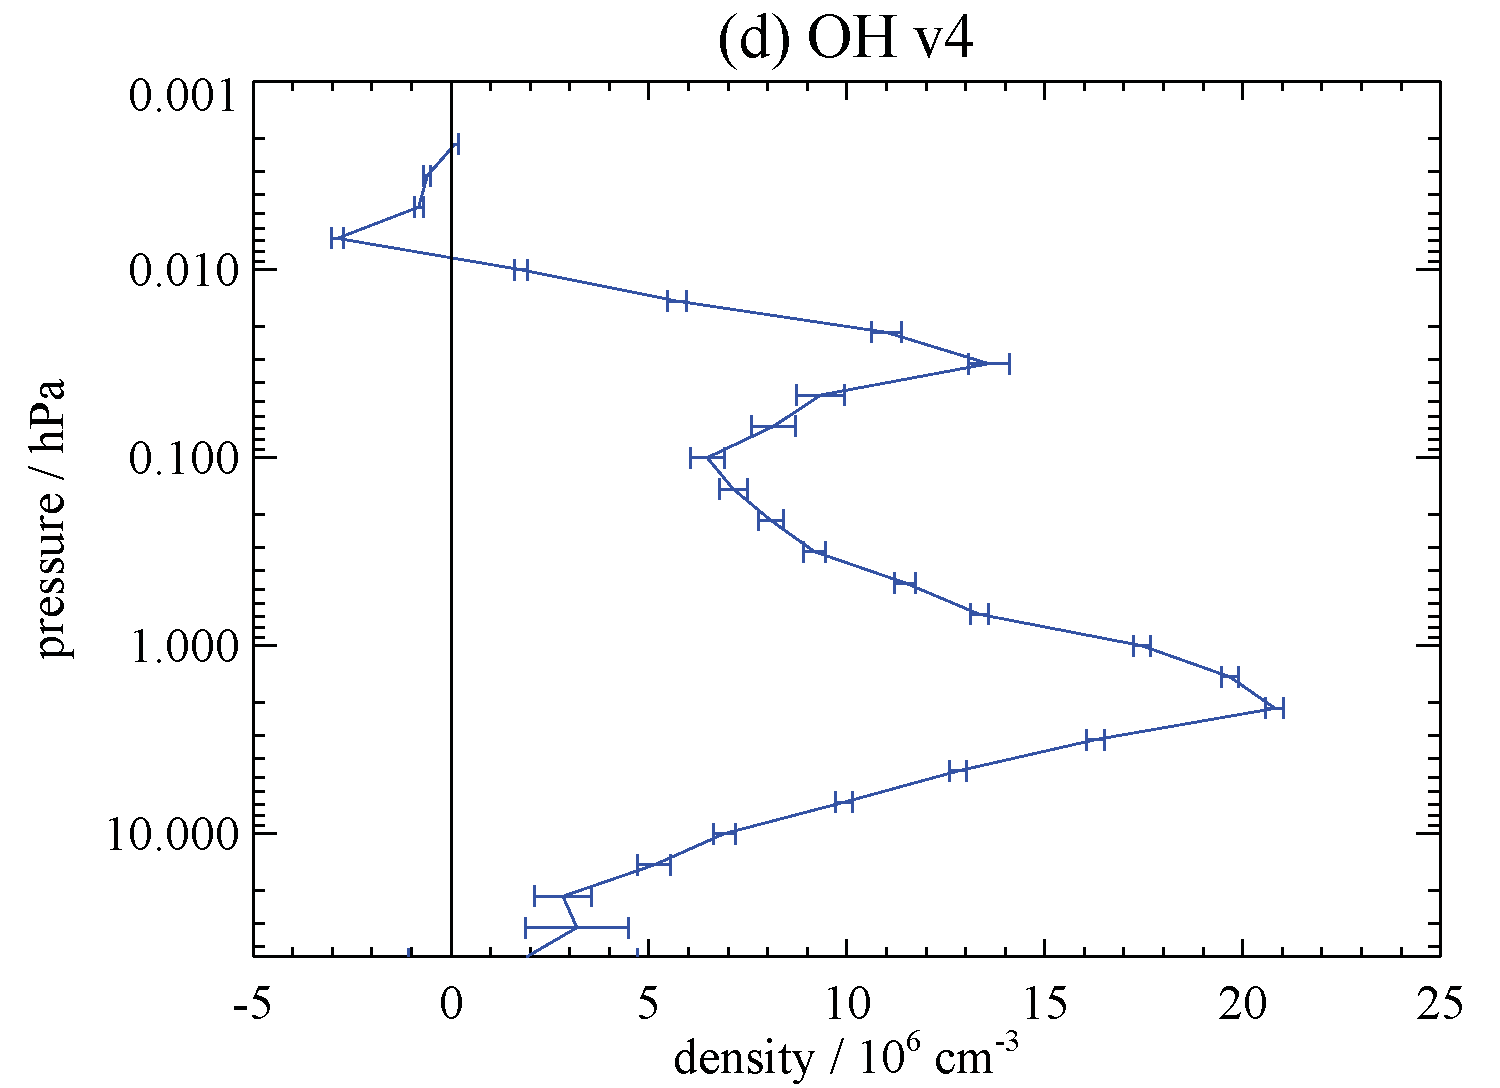
\includegraphics[width=0.5\linewidth]{figures/plot-OHv4-d}\\
\includegraphics[width=0.5\linewidth]{figures/plot-OHv3-e}&
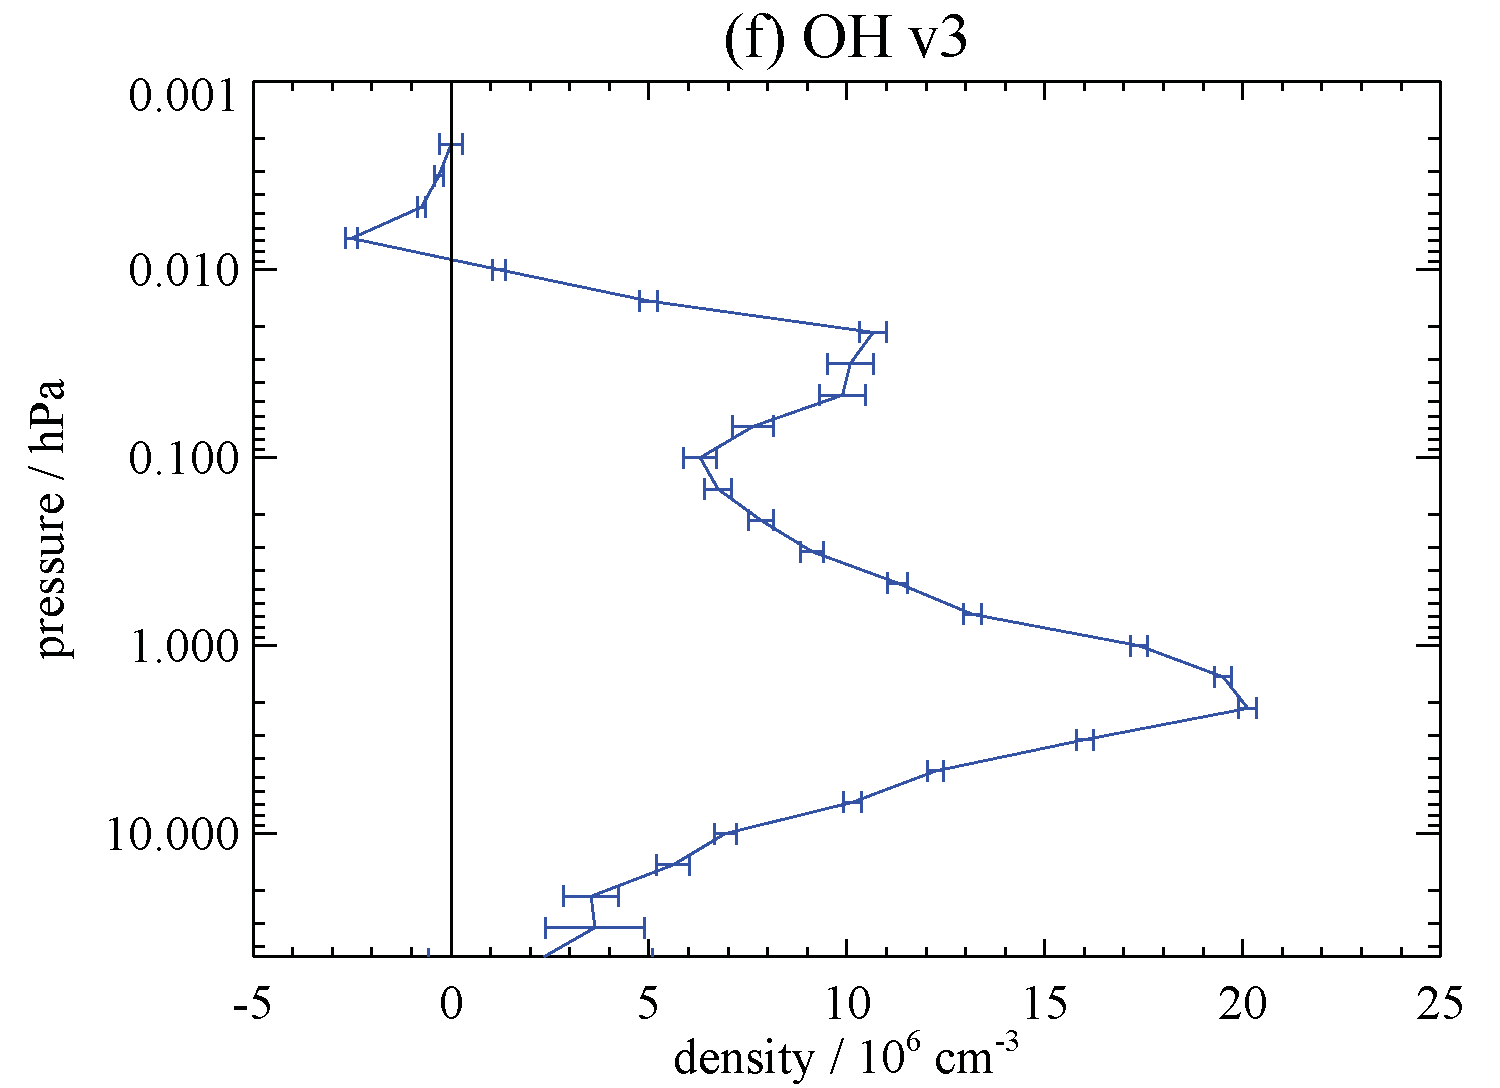
\includegraphics[width=0.5\linewidth]{figures/plot-OHv3-f}%
\end{tabular}
\caption{Zonal mean of retrieved OH and its estimated precision
  (horizontal error bars) for September 20, 2005 averaged over 29\degsym
  N to 39\degsym N\@. The average includes 98 profiles. Panel (a) shows
  \thisv OH vmr vs. pressure for day (black) and night (blue).  Panel (b)
  shows the same data plotted for the stratosphere. The retrieved night
  OH concentration is near zero for altitudes below 1\,hPa.  Panel (c)
  shows the same data in (a) converted into density units.  Panel (d)
  shows the day-night differences for the data in panel (c).  Note that
  the day-night difference is required for altitudes below 20\,hPa.
  Panels (e) and (f) are equivalent to (c) and (d) but using \prevv OH
  data.}
\label{fig:OHprofiles}
\end{figure}


\subsection{Accuracy}

Table~\ref{tab:OHSummary} summarizes the accuracy expected for OH\@.
The effect of each identified source of systematic error on MLS
measurements of radiance has been quantified and modeled
\citep{ReadEtal:2007}. These quantified effects correspond to either
$2\sigma$ estimates of uncertainties in each MLS product, or an estimate
of the maximum reasonable uncertainty based on instrument knowledge
and/or design requirements.These accuracy calculations were performed
with more realistic OH atmospheric profiles than for \prevv
estimates. Biases can be eliminated by taking day-night differences from
32\,--\,21\,hPa. For 15\,--\,0.1\,hPa, the observed night OH
concentration is small and day-night differencing is not ordinarily
needed. The overall uncertainty is the square root of the sum of squares
of the precision and accuracy.

\subsection{Data screening}
\label{sec:OHScreening}
It is recommended that OH data values be used in scientific
investigations if all the following tests are successful:

\begin{description}
\item[Pressure range:] \screeningrule{32\,--\,0.0032\,hPa.}
  \standardrangestatement
\standardprecisionrule
\evenstatusrule
\item[Quality:] \screeningrule{MLS \thisv OH data can be used
    irrespective of the value of the \texttt{Quality} field.}
\item[Convergence:] \convergencerule{1.1}
\end{description}

\subsection{Artifacts}

For some seasons, the Gas Laser Local Oscillator (GLLO) for the THz
receiver is automatically ``relocked'' as many as 5 times during a day,
leading to data gaps.  In these cases the \texttt{Status} flag is set to
\texttt{257} and the profile is ignored. This can present a problem when
compiling maps, because the missing data may appear at the same latitude
and longitude on successive days.

\subsection{Review of comparisons with other datasets}

Data from MLS v2.2 software have been validated with two balloon-borne
remote-sensing instruments and with ground-based column measurements.
Details of the comparison are given in \citet{PickettEtal:2008} and
\citet{WangEtal:2008}.  The comparison among v2.2, \prevv, and \thisv show
no significant differences except for the mesosphere where \thisv OH
daytime values are somewhat larger and less noisy in the summer
hemisphere (or tropics when near equinox).

\begin{table}
\caption{Summary of precisions, resolution, and uncertainties for the
  MLS OH product}
\vspace{\tablecaptionsep}
\label{tab:OHSummary}
\begin{minipage}{\textwidth}\small
\centering\begin{tabular}{rcccl}
\toprule
\textbf{Pressure} &
\parbox{6em}{\bfseries\centering Resolution\\ V $\times$ H /km} &
\parbox{5em}{\bfseries\centering Precision\footnote{Precision on an
    individual profile} (day/night) / 10\cp6 cm\cp{$-$3}} &
\parbox{5em}{\bfseries\centering Accuracy / 10\cp6 cm\cp{$-$3}} &
\textbf{Comments}\\
\midrule
$<$0.003\,hPa     & ---                  & ---                  & ---   &  Unsuitable for scientific use\\
0.003\,hPa        & 5.0 $\times$ 220     & 0.5 / 0.5            & 0.5 & \\
0.01 \,hPa        & 2.5 $\times$ 180     & 1.1 /1.1             & 2   & \\
0.1\,hPa          & 2.5 $\times$ 165     & 3.3 / 0.6            & 1.0  & \\
1.0\,hPa          & 2.5 $\times$ 165     & 1.9 / 0.4            & 1.0  & \\
10 \,hPa          & 2.5 $\times$ 165     & 2.3 / 1.4            & 0.9  & \\
32\,--\,14\,hPa   & 2.5 $\times$ 165     & 6\,--\,10 / 4\,--\,8 & 1.3  & Use day--night difference \\
$>$32\,hPa        & ---                  & ---                  & ---   & Unsuitable for scientific use\\
\bottomrule
\end{tabular}
\end{minipage}
\end{table}

%%% Local Variables:
%%% mode: latex
%%% TeX-master: "v5-x-report"
%%% End:

\speciestitle{Relative Humidity with respect to Ice}{RHI}{RHI}{
  \item[Useful range:] UTRHI, mean layer value for P $\le$ 383\,hPa, Profile from 316--0.001\,hPa.
  \item[Product lead:] William Read, \email{william.g.read@jpl.nasa.gov}}

\subsection{Introduction}

The vertical grid for the relative humidity with respect to ice (RHI) product is 12 levels per decade change in pressure for 1000--1.0\,hPa thinning to 6~levels per decade for 1.0--0.1\,hPa and finally 3~levels per decade for 0.1--10\cp{$-$5}\,hPa. The RHI product is a fusion of results from two separate retrievals. From 1000--383\,hPa, RHI is retrieved directly from optically thick radiances using measurement and retrieval principles similar to those employed by nadir sounding humidity receivers (e.g., TOVS). All grid levels between 1000--383\,hPa are filled with a uniform ``UTRHI'' (upper tropospheric relative humidity with respect to ice) value, representing the mean value of a broad layer (\mytexttilde4--6\,km) that peaks between \mytexttilde350\,hPa (in the moist tropics) and \mytexttilde650\,hPa (typical for dry high latitudes). This humidity is used as a lower altitude constraint and a priori for the vertically resolved humidity product that begins at 316\,hPa. From 316--10\cp{$-$5}\,hPa, RHI is derived from the standard products of water mixing ratio and temperature using the Goff-Gratch ice humidity saturation formula. RHI validation is presented in \citet{ReadEtal:2007}. Table~\ref{tab:RHISummary} is a summary of the RHI precision, resolution, and accuracy. The precision and accuracy figures for \thisv have been updated based upon systematic error analysis results described in \citet{ReadEtal:2007}. Some errors and footnote labels were discovered while performing this investigation that are present in \prevv have been corrected in Table~\ref{tab:RHISummary} for \thisv.

\subsection{Changes from \prevv}

There are no changes between \thisv and \prevv for the UTRHI (1000--383\,hPa) retrieval approach. RHI for pressures $\le 316\,$hPa is a derived product, and any changes reflect those in the input \ch{H2O} (\ref{sec:StandardH2O}) and temperature (\ref{sec:StandardTemperature}) products.

\begin{figure}
  \begin{center}
    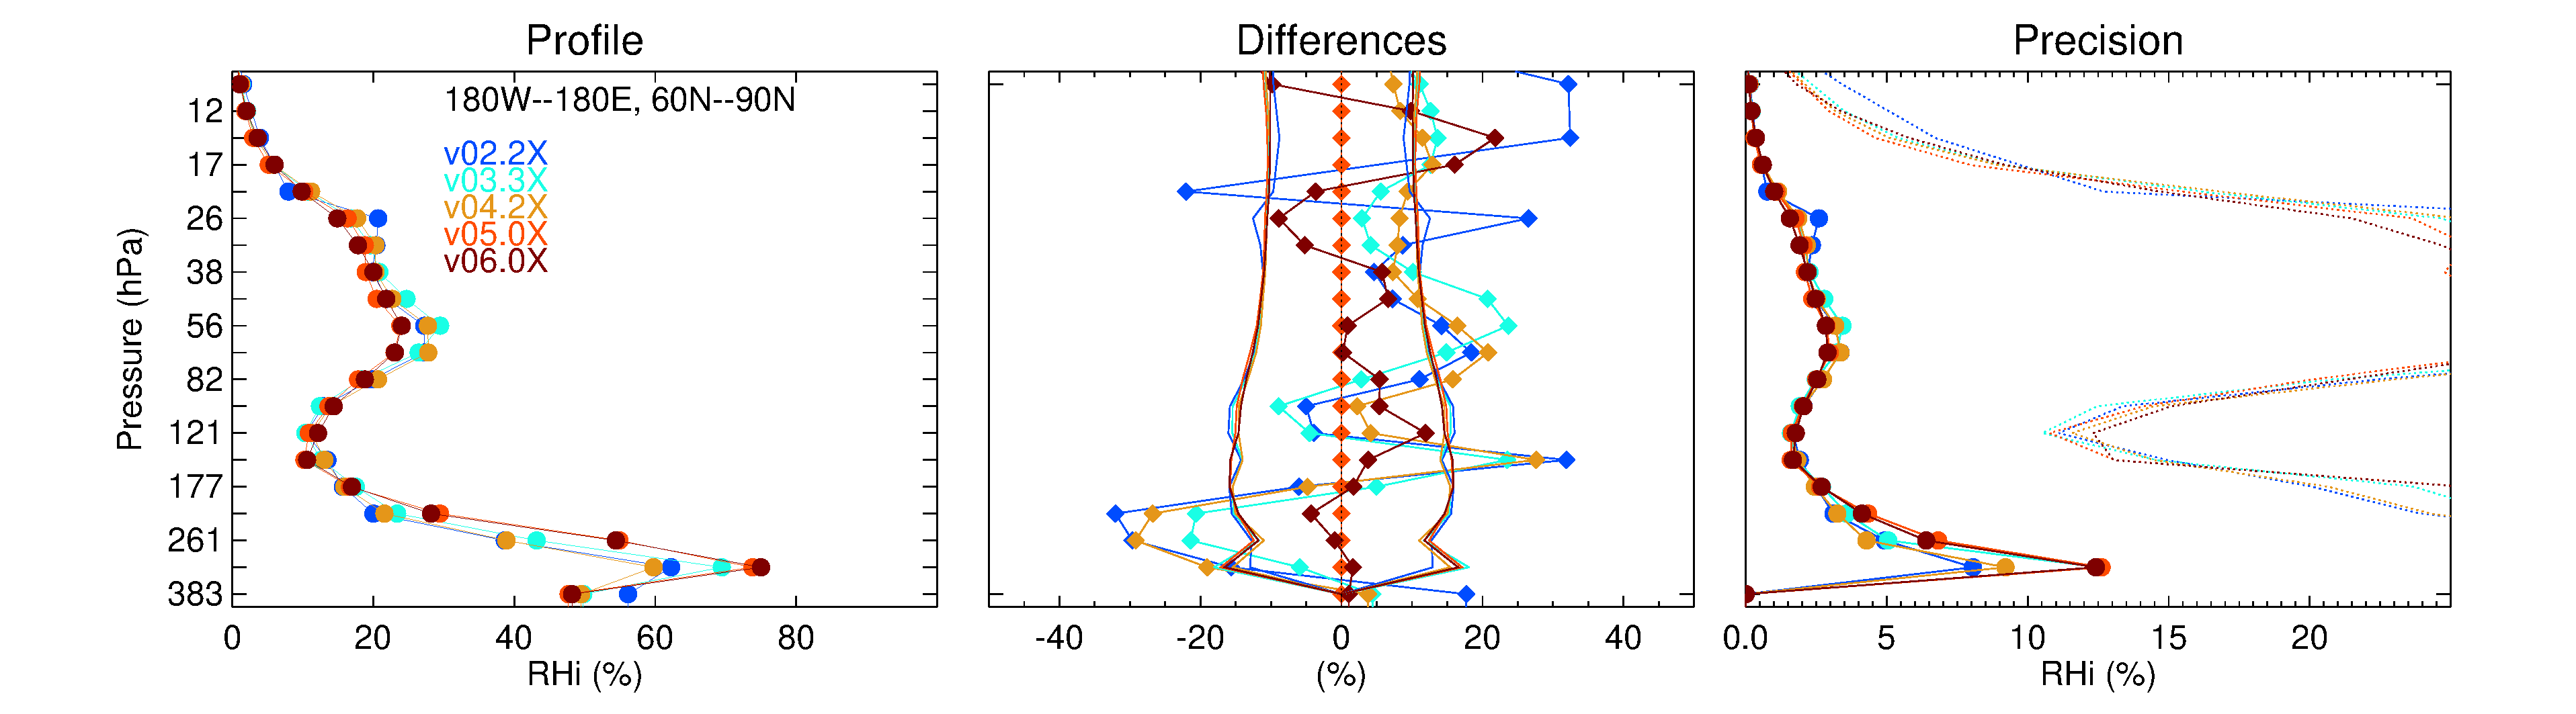
\includegraphics[width=0.8\linewidth]{figures/mls_rhi_v2-v3-v4-v5-v6_prfl_60n-90n.pdf}
    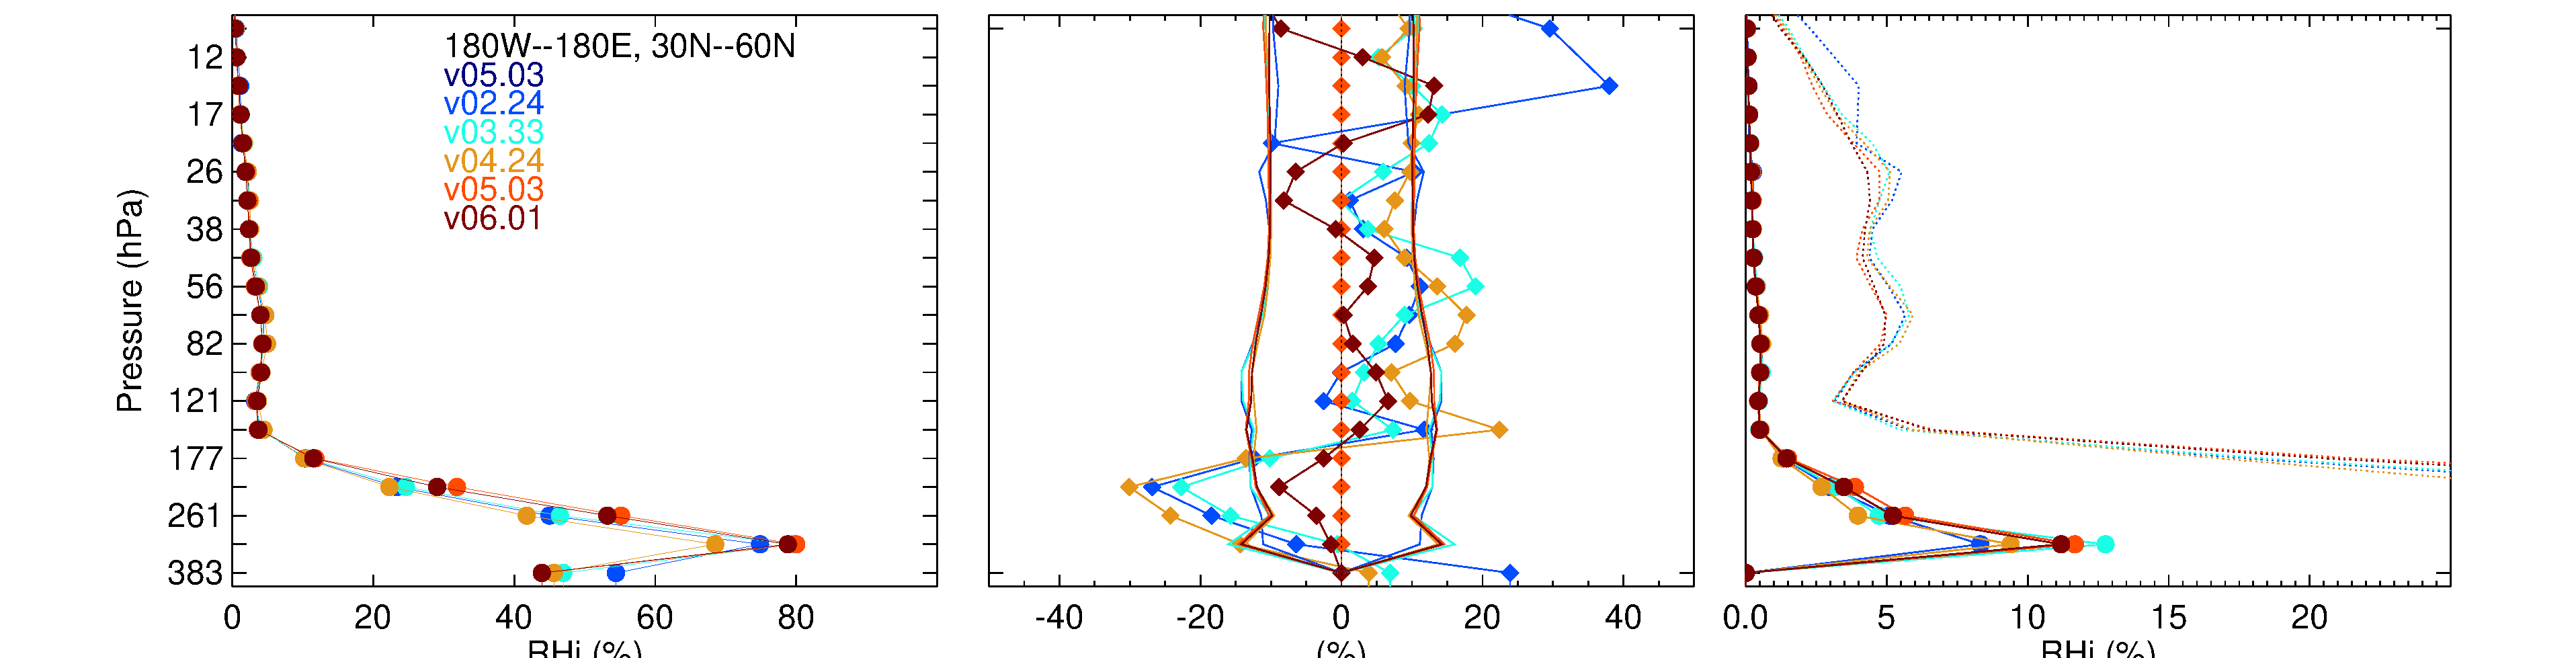
\includegraphics[width=0.8\linewidth]{figures/mls_rhi_v2-v3-v4-v5-v6_prfl_30n-60n.pdf}
    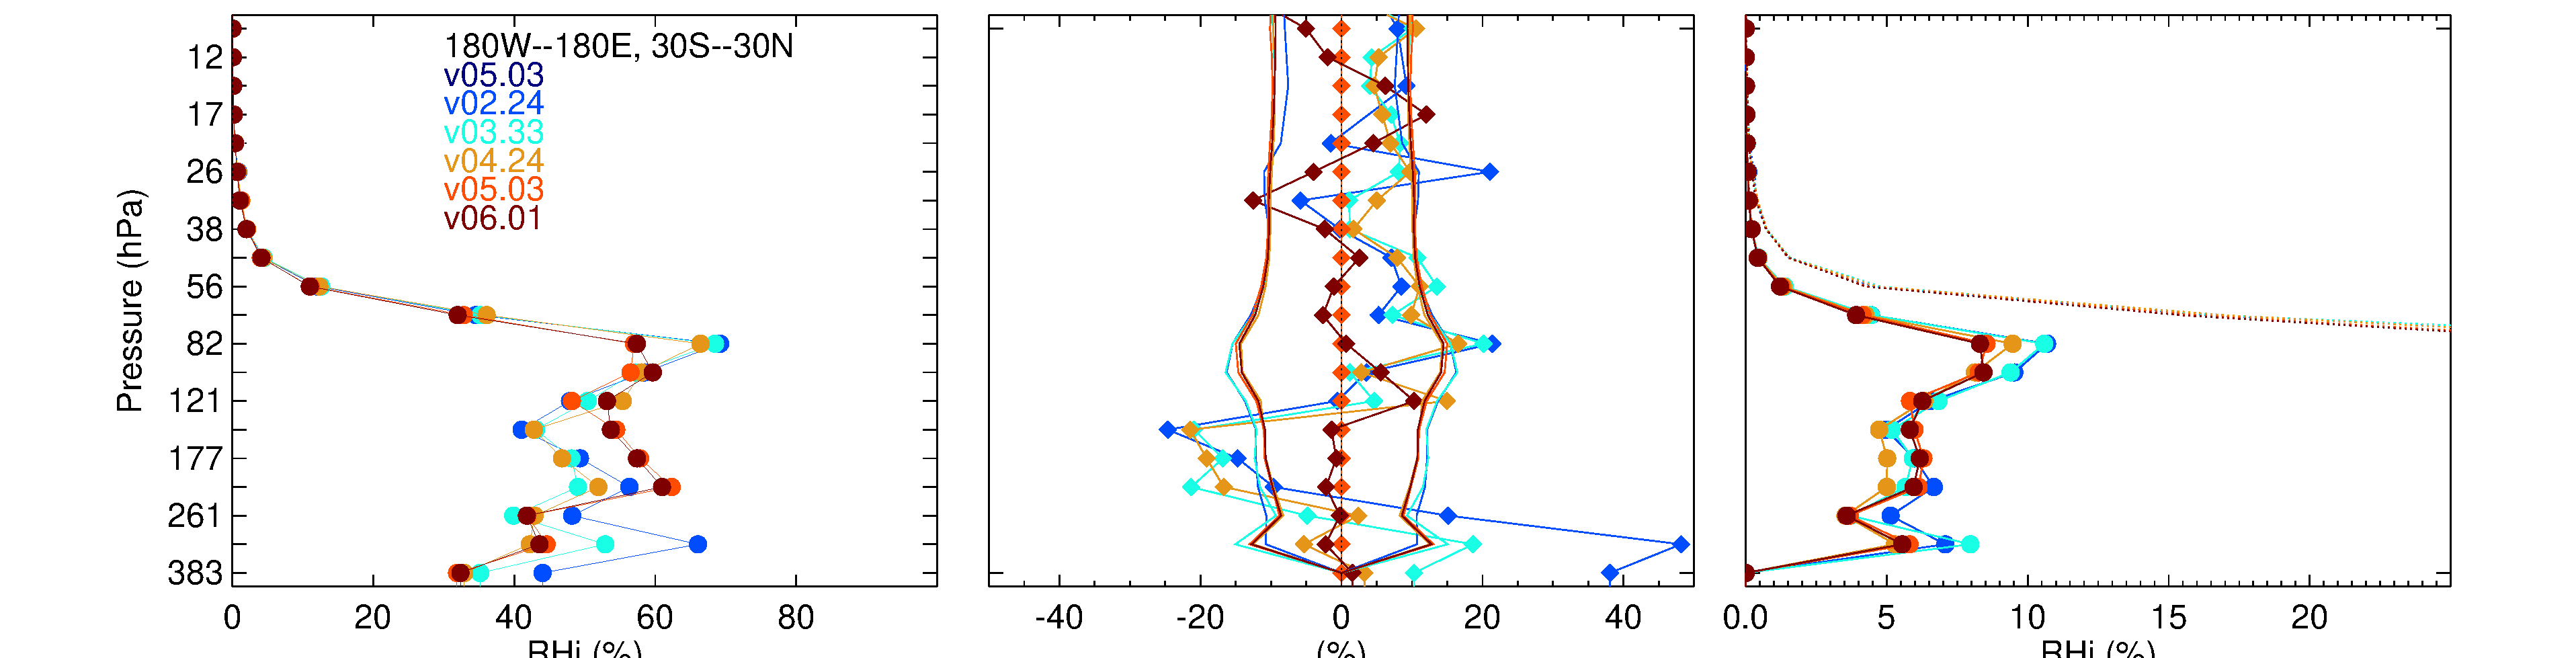
\includegraphics[width=0.8\linewidth]{figures/mls_rhi_v2-v3-v4-v5-v6_prfl_30s-30n.pdf}
    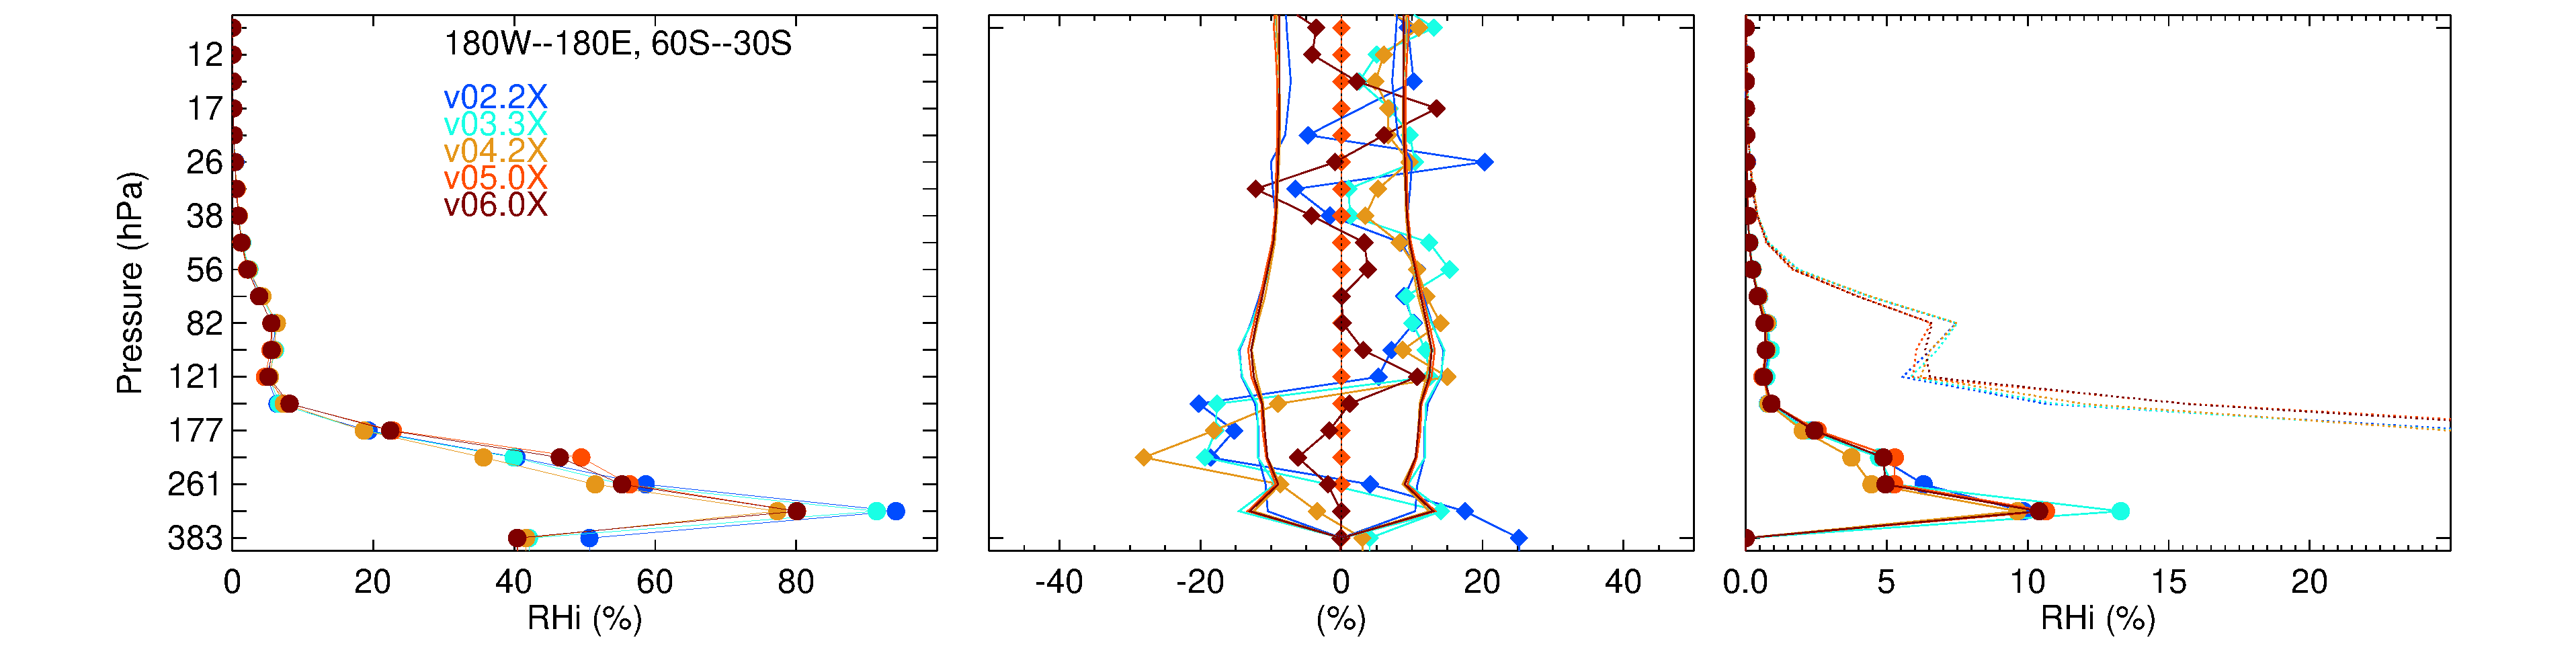
\includegraphics[width=0.8\linewidth]{figures/mls_rhi_v2-v3-v4-v5-v6_prfl_60s-30s.pdf}
    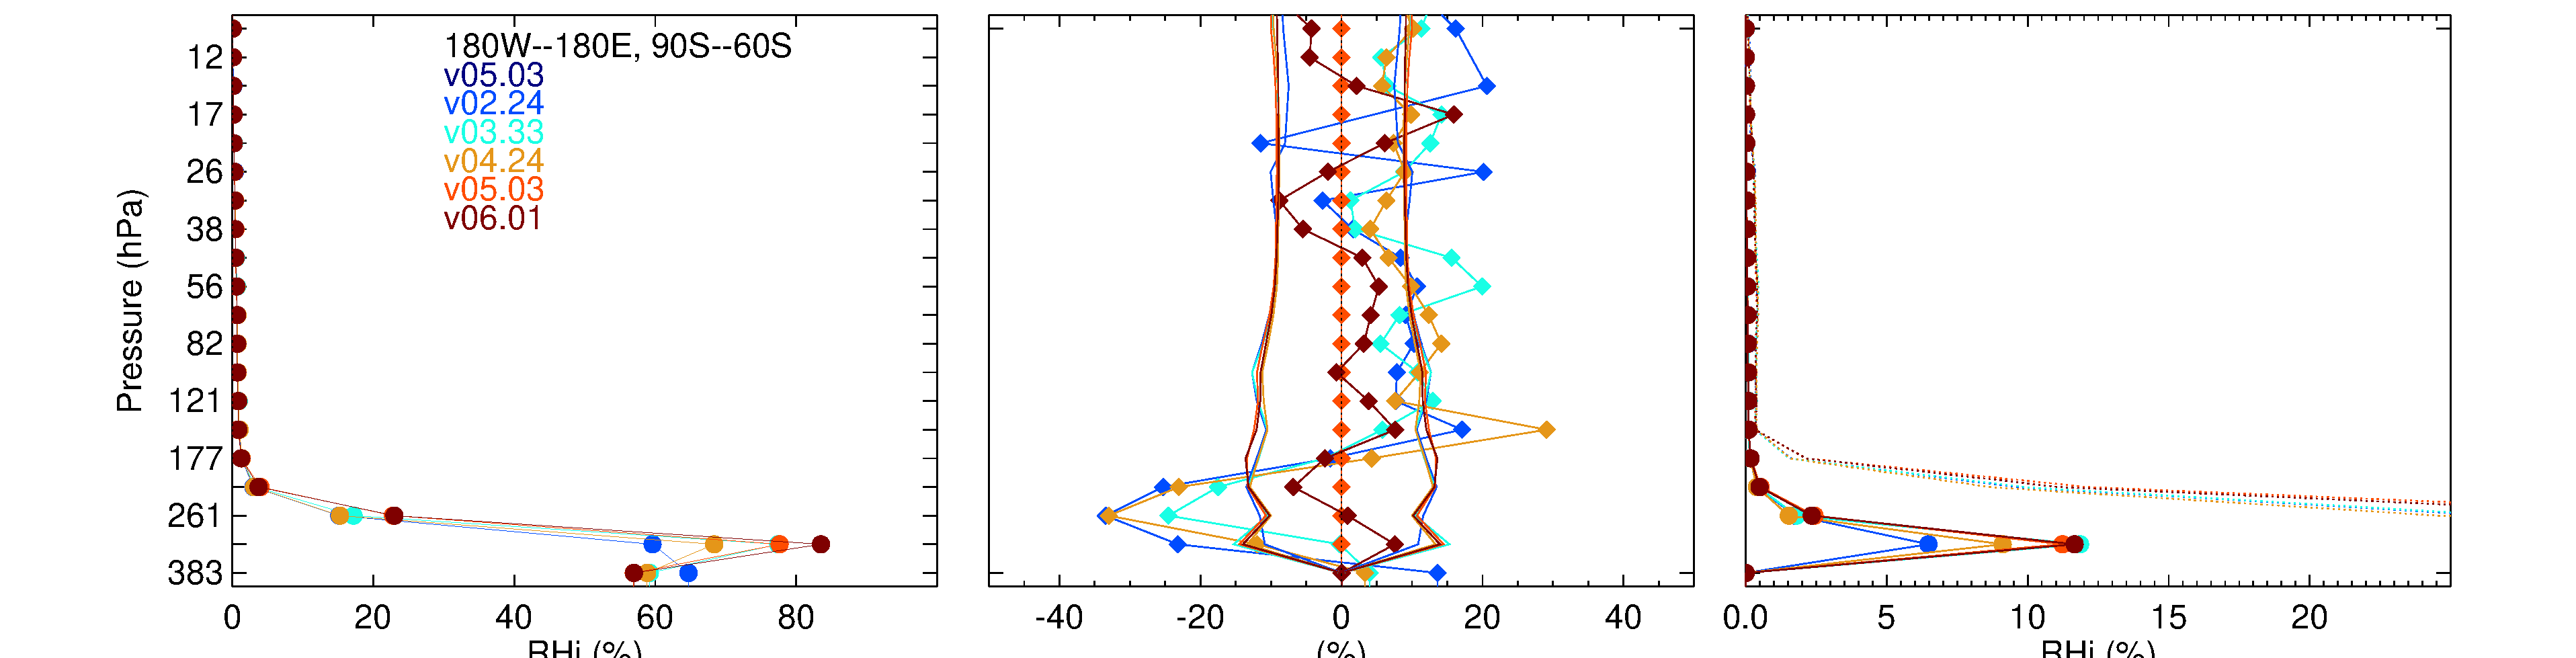
\includegraphics[width=0.8\linewidth]{figures/mls_rhi_v2-v3-v4-v5-v6_prfl_90s-60s.pdf}
  \end{center}
  \caption{\mycomment{Figures ovely trimmed at the bottom} A zonal mean comparison of RHI profiles in five latitude bands. v2.2x (blue), \viii (cyan), \viv (mustard), v5.0x (dark blue/orange), and v6.01 (dark red). RHI for Jan-Feb-Mar 2005.  Other time periods are similar. The left panel shows the mean profiles, the center shows the mean difference from v5.0x (blue, cyan, mustard, orange and red lines with diamonds). The colored lines without symbols are each versions' estimated precision. The right panel shows the estimated retrieval precision (solid lines with bullets) and measured variability (dotted lines) which includes atmospheric variability about the mean profile. X-axes are RHi in percent, y-axis are pressure in hPa. \mycomment{Why two lines for v5x, both dark blue and orange?}}
  \label{fig:avgmlsRHIprflcomp}
\end{figure}

Figure~\ref{fig:avgmlsRHIprflcomp} compares MLS v6.0, v4.2, v3.3, and \vii to v5.0. The changes seen in here reflect changes in temperature resulting from adjustments made to the filter shapes in the temperature-sounding channels and from changes in \ch{H2O} resulting from an adjustment to the MLS 190\nobreakdash-GHz radiance observations to improve the \ch{N2O} product.

Relative humidity data at pressures greater than 316\,hPa are derived from a broad layer relative humidity retrieval (using low-limb-viewing MLS wing channel radiances) similar to that obtained from NOAA operational humidity sounders such as TOVS\@. As noted in \citep{ReadEtal:2007}, the \vii retrieval at these pressures was likely to be \mytexttilde30\% too high, based on comparisons with AIRS\@. The accuracy of this retrieval is highly sensitive to the assumed transmission efficiency of the MLS optics system. In v3.3 this was adjusted empirically (within the uncertainty range established from MLS calibration) to give better agreement with AIRS in the tropics. In v4 the N\cs2 continuum was adjusted only for this phase to minimize the clear sky cloud induced radiance bias. Other than changes to sideband fractions and pointing offsets detailed in section~\ref{sec:StandardH2O}, no specific changes are implemented for v5 and v6. This retrieval is used as an a priori and profile constraint for the humidity profile at pressures greater than 316\,hPa which are not retrieved in the standard \ch{H2O} product retrieval.

The third panel in Figure~\ref{fig:avgmlsRHIprflcomp} shows the mean estimated single profile precision and the measured variability (which includes instrument noise and atmospheric variability). All the versions show very similar precision, and in the lower stratosphere and upper troposphere these precision uncertainties are much smaller than the measured atmospheric variability. The precision for 383\,hPa (and larger pressures) is reported in the \texttt{L2GP} as 0\% by mistake. The actual precision is typically 0.2\%.

\subsection{Resolution}

RHI for pressures of 316\,hPa and smaller is a derived product and therefore a retrieval averaging kernel is not directly available. An estimate for the spatial resolution (vertical \texttimes along track) of this product is a convolution of the temperature and \ch{H2O} resolutions. Typically \ch{H2O} has the poorer horizontal resolution and temperature has the poorer vertical resolution. Therefore, as a first-order estimate of spatial resolution, the horizontal resolution of the \ch{H2O} product should be assumed, along with the vertical resolution for temperature (see \ref{sec:StandardH2O} and \ref{sec:StandardTemperature}). The cross track resolution is probably 12\,km, the larger of the temperature and \ch{H2O} cross track resolutions. These resolutions are only true in the limit that the mean $\log$(\ch{H2O}) doesn't change appreciably over the broader temperature measurement volume. The longitudinal separation of the MLS measurements, set by the Aura orbit, is 10\degsym--\,20\degsym\ over middle and lower latitudes, with much finer sampling in polar regions.

The RHI for pressures greater than 316\,hPa, represents a mean value in a broad layer (4--6\,km) whose sensitivity peaks between \mytexttilde350\,hPa (in the moist tropics) and \mytexttilde650\,hPa (typical for dry high latitudes).

\subsection{Precision}

The values for precision are the root sum square (RSS) precisions for \ch{H2O} and temperature propagated through the Goff-Gratch relationship, see sections~\ref{navSectionH2O} and~\ref{navSectionTemperature} for more details. The precisions are set to negative values (or zero in some cases) in situations when the retrieved precision is larger than 50\% of the a priori precision for either temperature or \ch{H2O} --- an indication that the data is biased toward the a priori value. The precisions for levels between 1000 and 383~hPa (vertical levels 1--6) are reported as 0\% by error. It should typically be 0.2\% and is the same value for all levels between 1000 and 383~hPa.

\subsection{Accuracy}

The values for accuracy are the RSS accuracies for \ch{H2O} and temperature scaled into \%\,RHI units. see sections~\ref{sec:StandardH2O} and~\ref{sec:StandardTemperature} for more details.

\begin{nofloatpages}
\subsection{Data screening}
\label{sec:RHIScreening}
\begin{description}

  \item[Pressure range:] \screeningrule{Profile from 316--0.001\,hPa, larger pressures represent mid/upper troposphere column.} \standardrangestatement \standardprecisionrule \evenstatusrule

  \item[Clouds:] Ignore status bits 16 (high clouds) or 32 (low clouds) set indicating the presence of clouds. See artifacts for more details.

  \item[Quality field:] \screeningrule{The \texttt{Quality} fields for both the \texttt{L2GP-RHI} and \texttt{L2GP-Temperature} swaths need to be considered, as described below:}
    \begin{description}
      \item[For pressures of 83\,hPa and smaller:] Use only profiles with RHI \texttt{Quality} \emph{greater} than 0.7 and Temperature \texttt{Quality} \emph{greater} than 0.2
      \item[For pressures of 100\,hPa and larger:] Use only profiles with RHI \texttt{Quality} \emph{greater} than 0.7 and Temperature \texttt{Quality} \emph{greater} than 0.9.
    \end{description}

  \item[Convergence field:] \screeningrule{Only profiles with a value of the RHI \texttt{Convergence} \emph{less} than 2.0 and Temperature \texttt{Convergence} \emph{less} than 1.03 should be used in scientific studies.}

  \item[Temperature precision:] The \texttt{L2gpPrecision} field in the \texttt{L2GP-Temperature} file can be used to further eliminate outliers that are believed to be the result of thick clouds, primarily in the tropics. If careful screening of the troposphere is required, levels 261--178\,hPa should be avoided if any of the following criteria are met:
    \begin{description}
      \item[At 316\,hPa:] \texttt{L2gpPrecision} $>1.1$\,K \textbf{and} latitude $> -60$\degsym
      \item[At 261\,hPa:] \texttt{L2gpPrecision} $>0.7$\,K
      \item[At 215\,hPa:] \texttt{L2gpPrecision} $>0.825$\,K
    \end{description}

  \item[Additional screening for based on \ch{H2O}:] Eliminate highly oscillatory profiles by eliminating \ch{H2O} profiles having values less than 0.101\,ppmv at any pressure $< 1$\,hPa (vertical levels 1--37).
\end{description}
\end{nofloatpages}
\subsection{Artifacts}

See sections~\ref{sec:StandardH2O} for \ch{H2O} and~\ref{sec:StandardTemperature} for temperature for specific issues related to these parent products. Effects of MLS temperature precision (\mytexttilde1--2\,K) must be considered if one wishes to use MLS RHI to study supersaturation. In simulation studies, systematic errors (such as tangent pressure retrieval and errors), in addition to introducing biases, also increase variability in differences with respect to a ``truth'' data set particularly for pressures greater than 200\,hPa. This will add to the frequency of supersaturation in the tail of MLS RHI distribution functions. Therefore, MLS RHI is not recommended for studying statistics of supersaturation at pressures greater than 178\,hPa. For smaller pressures, one must remove the contribution from temperature noise as part of the analysis. Measurements taken in the presence of clouds significantly degrade the precision, that is increases the scatter about the mean, but the mean bias as compared to AIRS changes by less than 10\%.  Also, users should note the possibility of a potential drift in the MLS lower stratospheric water vapor product, discussed in sections~\ref{sec:R2DutyCycling} and~\ref{sec:H2OChanges}. Such a drift will also impact the RHI product.

\subsection{Review of comparisons with other datasets}

Figures~\ref{fig:RHIairsmlsjfm2009maps} and \ref{fig:RHIairsmlsjja2009maps} show comparisons between AIRS v6 and MLS \vii, v3.3, v4.2, v5.0, and v6.0. Mapped features tend to agree well but MLS produces higher relative humidities in the moist regions of the tropics relative to AIRS. One noteworthy feature is that at high latitudes at 200 and 250~hPa, v6 and v5 have higher relative humidity than previous versions that was an effort to adress a likely dry bias in the MLS \ch{H2O} retrieval.

\begin{figure}
  \begin{center}
    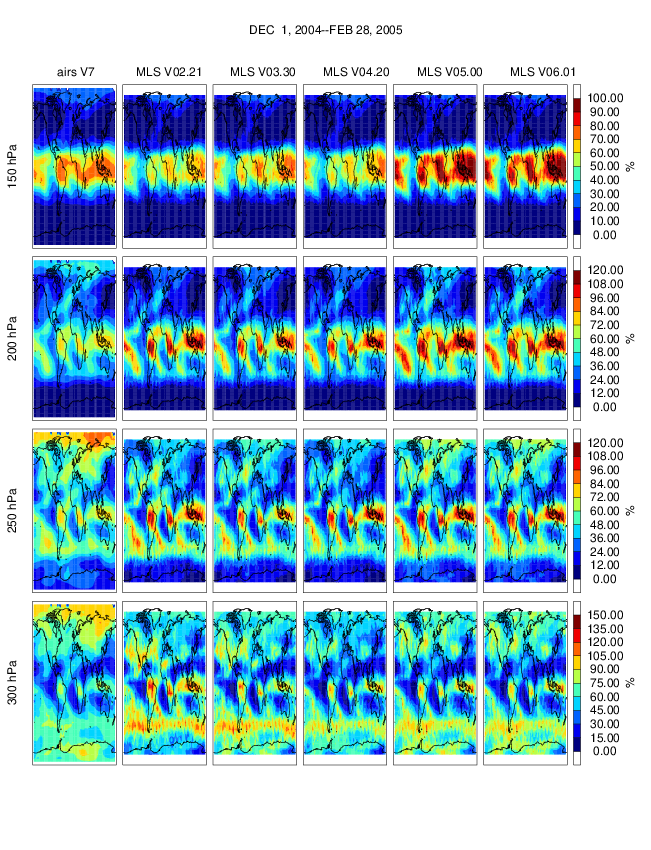
\includegraphics[width=0.9\linewidth, trim=0mm 24mm 0mm 8mm]
    {figures/rhi_grid_maps_djf2005_airsv7-mlsv2-v6.png}
  \end{center}
  \caption{Mapped RHi fields from AIRS v7 (left panel), MLS \vii (2nd from left), MLS v3.3 (3rd from left), MLS v4.2 (3rd from right), MLS v5.0 (2nd from right), and MLS v6.0 (right panel) pressures between 300--150 hPa for December, January, and
    February 2005.}
  \label{fig:RHIairsmlsjfm2009maps}
\end{figure}

\begin{figure}
  \begin{center}
    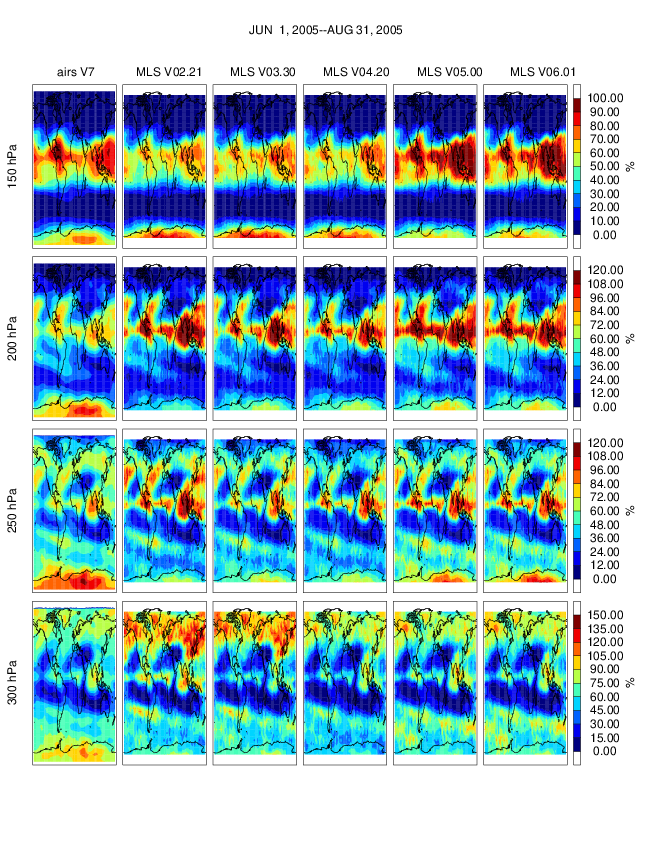
\includegraphics[width=0.9\linewidth, trim=0mm 24mm 0mm 8mm]
    {figures/rhi_grid_maps_jja2005_airsv7-mlsv2-v6.png}
  \end{center}
  \caption{Mapped RHi fields from AIRS v7 (left panel), MLS \vii (2nd from left), MLS v3.3 (3rd from left), MLS v4.2 (3rd from right), MLS v5.0 (2nd from right), and v6.0 (right panel) pressures between 300--150 hPa for June, July, and August 2005.}
  \label{fig:RHIairsmlsjja2009maps}
\end{figure}

\subsection{Desired improvements}

While many defects in v4.2 and earlier versions have been addressed, further investigation into their effectiveness, especially the drift reduction and high latitude low value retrievals in the upper troposphere needs to be assessed and improved upon if necessary. Retrieval of vertically resolved \ch{H2O} for pressures $>316$\,hPa may be possible at high latitudes during dry conditions, but that remains to be investigated.

\begin{table}
  \caption{Summary of MLS \thisv UTLS RHI product.}
  \vspace{\tablecaptionsep}
  \label{tab:RHISummary}
  \begin{minipage}{\linewidth}
    \centering\begin{tabular}{ccccl}
\toprule
\parbox[m]{5em}{\bfseries\centering Pressure \newline\newline hPa} &
\parbox[m]{5.5em}{\bfseries\centering Resolution%
\footnote{Vertical and along-track horizontal resolutions; cross-track horizontal resolution is \mytexttilde9\, km.}
V~$\times$~H \newline km} &
\parbox[m]{7em}{\bfseries\centering Single profile \newline precision
\footnote{Fractional error ([error in RHI] / RHI) in percent} \newline \%} &
\parbox[m]{7em}{\bfseries\centering Accuracy \footnote{Fractional error ( [error in RHI] / RHI) in percent}\newline\newline \%} &
\parbox[m]{7em}{\bfseries\centering Comments \newline\newline}
\\ \midrule
0.00046 & --- & ---  & --- & Unsuitable for scientific use \\  
0.001 & 13.9 $\times$ 708 & 184  & 76 &  \\
0.002 & 14.0 $\times$ 508 & 145  & 74 &  \\
0.004 & 14.7 $\times$ 428 & 88   & 49 & \\
0.010 & 13.8 $\times$ 398 & 66   & 37 & \\
0.022 & 12.0 $\times$ 374 & 53   & 40 & \\
0.046 & 10.6 $\times$ 318 & 42   & 41 & \\
0.10  & 8.0  $\times$ 270 & 38   & 37 & \\
0.22  & 8.2  $\times$ 262 & 28   & 26 & \\
0.46  & 8.3  $\times$ 261 & 17   & 17 & \\
1.00  & 7.2  $\times$ 316 & 12   & 11 & \\
2.15  & 6.9  $\times$ 308 & 10   & 17 & \\
4.64  & 6.1  $\times$ 295 & 10   & 18 & \\
10    & 5.5  $\times$ 291 & 10   & 14 & \\ 
22    & 5.3  $\times$ 275 & 11   & 33 & \\
46    & 5.3  $\times$ 267 & 12   & 16 & \\
68    & 5.4  $\times$ 248 & 12   & 23 & \\
83    & 5.6  $\times$ 248 & 13   & 27 & \\
100   & 5.8  $\times$ 251 & 12   & 30 & \\
121   & 5.6  $\times$ 259 & 11   & 55 & \\
147   & 5.1  $\times$ 259 & 11   & 51 & \\
178   & 5.0  $\times$ 263 & 10   & 51 & \\
215   & 4.5  $\times$ 263 & 10   & 61 & see Table~\ref{tab:H2OSummary} \\
261   & 4.7  $\times$ 253 & 9   & 80 & see Table~\ref{tab:H2OSummary} \\
316   & 4.4  $\times$ 253 & 13   & 167 & see Table~\ref{tab:H2OSummary} \\
UTRHI, $>$316 & 6 $\times$ 155 & 40(est) & 10(est) & measurement height
depends \\
&                &    &     &   on atmospheric humidity \\
\bottomrule
\end{tabular}
  \end{minipage}
\end{table}

\speciestitle{Sulfur Dioxide}{SO\cs2}{SO2}
\begin{description}
\item[Useful range:] 215\,--\,10.0\,hPa
\item[Contact:] William Read, \email{William.G.Read@jpl.nasa.gov}
\end{description}

\subsection*{Introduction}

The standard SO\cs2 product is taken from the 240-GHz retrieval. MLS can
only measure significantly enhanced concentrations above nominal
background such as that from volcanic injections.  SO\cs2 has not yet
been validated.

\subsection*{Changes from v2.2}

The \thisv SO\cs2 retrieval will be impacted by the addition of interline
interference terms in the O\cs3 line shape model, an updated CO line
width parameter, and using a different set of 240\,GHz channels.
Another \thisv change is the spectral baseline treatment that now uses a
frequency-squared extinction term, configured as a relative
humidity-like (RH) species. The RH treatment responds better to high
extinction conditions when the middle troposphere is very humid. This
enhancement eliminated a high bias in 316\,hPa O\cs3 in the tropics that
is present in v2. An unfortunate side effect of the RH baseline is that
it is more adversely affected by clouds, causing spikes in the retrieval
of R3 products including SO\cs2.

\subsection*{Resolution}
\onestandardavk{SO2}{SO\cs2}%

Based on Figure~\ref{fig:AvkSO2}, the vertical resolution for SO\cs2 is
\texttildelow3\,km and the horizontal resolution is 170\,km. The horizontal
resolution perpendicular to the orbit track is 6\,km for all pressures.

\subsection*{Precision}

The estimated precision for SO\cs2 is \texttildelow3\,ppbv for all heights
between 215\,--\,10\,hPa. The precisions are set to negative values in
situations when the retrieved precision is larger than 50\% of the a
priori precision -- an indication that the data is biased toward the a
priori value.

\subsection*{Accuracy}

The values for accuracy are based on the approach used for the v2.2
systematic error analysis performed on the MLS measurement system
\citep{ReadEtal07}, updated for \thisv. The accuracy is estimated to be
\texttildelow5\,ppbv for pressures less than 147\,hPa increasing to
\texttildelow20\,ppbv at 215\,hPa.

\subsection*{Data screening}
\begin{description}
\item[Pressure range:] \screeningrule{215\,--\,10.0\,hPa} \standardrangestatement
\item[Estimated Precision:] \screeningrule{Values with negative
    precision can be used, though with caution.}

  Although it is generally recommended not to use values where precision
  is flagged negative, SO\cs2 is an exception and it is OK to use values
  with negatively flagged precision (provided that the entire profile is
  not so flagged). High retrieved values of SO\cs2 at the higher
  pressures (e.g. 215 and 147~hPa) will also have larger precision
  values which are sometimes large enough to trigger the ``too much \emph{a
    priori} influence'' flag. While a priori influence is present and
  the retrieved value is probably smaller than reality because the
  retrieval is being pulled towards the a priori value of zero, this
  does not detract from the fact that greatly enhanced SO\cs2 is being
  reported, reflecting the detection of a plume.
\evenstatusrule
\item[Quality:] \qualityrule{0.6}
\item[Convergence:] \convergencerule{1.8}
\end{description}

\subsection*{Artifacts}

The product is unvalidated. There is a tendency for the \thisv SO\cs2
product, as for CO, to have spikes in the presence of clouds.

\subsection*{Review of comparisons with other datasets}

MLS has successfully detected SO\cs2 from 23 eruptions since launch.
These include Manam (Papua, New Guinea -- 3 events), Anatahan (Mariana
Islands), Sierra Negra (Galapogos Island), Soufriere Hills (Montserrat,
West Indies), Tunguraua (Ecuador), Rabaul (Papua New Guinea),
Nyamuragira (Congo), Piton de la Fournaise (Reunion Island), Jebel
al-Tair (Yemen), Okmok (Alaska), Kasatochi (Alaska), Dalaffilla
(Ethiopia), Redoubt (Alaska), Sarychev (Kuril Islands, Russia), Pacaya
(Guatamala), Merapi (Indonesia), Grimsvoth (iceland), Puyehue-Cordon
Calle (Chile), Nabro (Eritrea) and Paluweh (Indonesia).

\begin{figure}
\begin{center}
\dontincludegraphics[width=0.7\linewidth]{figures/kosatochi_11082008}
\dontincludegraphics[width=0.7\linewidth]{figures/kosatochi_12082008}
\end{center}
\caption{An overlay of MLS measurement tracks on an OMI SO\cs2
  measurement on 11 and 12 August 2008 (separate maps) showing the
  dispersial of SO\cs2 from the Kasatochi eruption (8 Aug 2008, black
  triangle). The color scale indicates the SO\cs2 column measured by
  OMI\@. The daytime MLS tracks are small open circles and the nighttime
  tracks are filled black. When the calculated column from MLS exceeds 1
  DU, that measurement is indicated by a larger open circle filled with
  the color of the column measurement as indicated by the color scale
  below (same as for OMI)\@. The panels at right show all the measured
  profiles covering the area shown in the maps for SO\cs2 and
  HCl. Profiles where the MLS column calculation exceeds 1 DU are
  highlighted in red.}
\label{fig:so2overlay}
\end{figure}

Figure~\ref{fig:so2overlay} shows an overlay comparison of column SO\cs2
measured by OMI and the same calculated by MLS for two days following
the Kasatochi eruption. It is clear that MLS detects the main plume
dispersal features. It also appears that MLS columns are much smaller
than those from OMI. Interpreting the significance of this is not
straightforward given that OMI has to make assumptions regarding the
profile shape and can observe SO\cs2 down to the boundary layer. The MLS
column begins at 215~hPa and integrates upward neglecting the
tropospheric contributions. Another limitation is that OMI can only make
measurements during the day whereas MLS can make them day and night.
Since the plume is moving relatively quickly over the 12 hour
measurement separation time, MLS nighttime measurements often miss
and/or detect plume features differently than OMI\@. MLS vertically
resolved measurement shows that this plume has separated into distinct
layers at different altitudes.  The altitude of SO\cs2 measured by MLS
usually coincides with the altitude of aerosols measured by CALIPSO,
providing supporting evidence for the validity of the
vertically-resolved MLS observations.

\begin{table}
\caption{Summary of MLS \thisv SO\cs2 product.}
\label{tab:SO2Summary}
\vspace{\tablecaptionsep}
\begin{minipage}{\linewidth}
\centering\begin{tabular}{ccccl}
\toprule
\parbox[m]{6em}{\bfseries\centering Pressure / hPa} &
\parbox[m]{6em}{\bfseries\centering Resolution V~$\times$~H \ km} &
\parbox[m]{8em}{\bfseries\centering Single profile precision
\footnote{Absolute error in percent} / ppbv} &
\parbox[m]{6em}{\bfseries\centering Accuracy / ppbv} &
\bfseries Comments \\
\midrule
$<$ 10 & --- & --- & --- &  Unsuitable for scientific use \\
     10 & 3 $\times$ 180 &  3.5 &  6  & \\
     15 & 3 $\times$ 180 &  3.5 &  3  & \\
     22 & 3 $\times$ 180 &  3.2 &  4  & \\
     32 & 3 $\times$ 180 &  3.2 &  5  & \\
     46 & 3 $\times$ 180 &  3.0 &  5  & \\
     68 & 3 $\times$ 180 &  3.0 &  6  & \\
    100 & 3 $\times$ 180 &  3.0 &  6  & \\
    147 & 3 $\times$ 180 &  3.1 &  10 & \\
    215 & 3 $\times$ 180 &  3.8 &  20 & \\
$>$215 & --- & --- & --- & Unsuitable for scientific use \\
\bottomrule
\end{tabular}
\end{minipage}
\end{table}


%%% Local Variables:
%%% mode: latex
%%% TeX-master: "v4-x-report"
%%% End:

\speciestitle{Temperature}{T}{Temperature}{%
\item[Useful range:] 261\,--\,0.001\,hPa
\item[Contact:] Michael J. Schwartz,
  \email{Michael.J.Schwartz@jpl.nasa.gov}}
\label{sec:StandardTemperature}%
\subsection*{Introduction}

The MLS \thisv temperature product is similar to the v2.2
product that is described in~\citet{SchwartzEtal08}.  MLS temperature
is retrieved from bands near O\cs2 spectral lines at
118\,GHz and 239\,GHz that are measured with MLS radiometers R1A/B and R3,
respectively.  
The isotopic 239-GHz line is the primary source of
temperature information in the troposphere, while the 118-GHz line is
the primary source of temperature in the stratosphere and above.  
MLS \thisv temperature has a \texttildelow\,$-$1\,K  bias with
respect to correlative measurements in the troposphere
and stratosphere, with 2\,--\,3\,K peak-to-peak additional systematic
vertical structure.  Table~\ref{tab:TSummary} summarizes the measurement
precision, resolution, and modeled and observed biases.  The following
sections provide details.

\subsection*{Differences between \thisv and v2.2 }
The MLS \thisv temperature retrieval algorithms are largely unchanged from
those of v2.2, using the same subsets of the same radiance bands, so the
resulting products are very similar. An exception is the \mbox{316-hPa}
level, which in \thisv is noisier and has larger biases relative to
analyses than in v2.2.  The \thisv temperature \mbox{316-hPa} level is not
recommended for scientific use.  Version \thisv has eight more retrieval
levels in the upper stratosphere, giving 12 levels per decade from the
surface to 1\,hPa.  Noise and biases have been reduced at ``chunk
boundaries'', the breaks between the 10-profile blocks of data that are
concurrently retrieved by the 2-D algorithms.  The non-convergence of
the retrieval over substantial sections of the polar autumn in v2.2 has
been eliminated in version \thisv.  Vertical smoothing has been reduced in
the mesosphere and lower thermosphere, improving vertical resolution at
a cost of less than a factor of two in precision, but also resulting in
what, in preliminary validation, appears to be some vertically
oscillating profiles in the mesopause region, particularly at the
equator. The \emph{a priori} temperature profiles used in \thisv are
consistently GEOS-5.2, while v2.2 used GEOS-5.1 before September of
2008.  GEOS-5.1 has a low bias in the upper stratosphere of
0\,--\,15\,K, particularly at high latitudes, and resulted in biases of
\texttildelow1\,K near the stratopause.

\subsection*{Resolution}
\onestandardavk{Temperature_HR}{Temperature}%
The vertical and horizontal resolution of the MLS temperature
measurement is shown by averaging kernels in
Figure~\ref{fig:AvkTemperature_HR}.  Vertical resolution, shown on the
left panel, is \texttildelow5\,km from 261\,hPa to 100\,hPa, improves to
3.6\,km at 31.6\,hPa and then degrades to 4.3\,km at 10\,hPa, 5.5\,km at
3.16\,hPa and 6\,km at 0.01\,hPa.  Along track resolution is
\texttildelow170\,km from 261\,hPa to 0.1\,hPa and degrades to 220\,km at
0.001\,hPa.  The cross-track resolution is set by the 6-km width of the
MLS 240-GHz field of view in the troposphere and by the 12-km width of
the MLS 118-GHz field of view in the stratosphere and above.  The
longitudinal separation of MLS measurements from a given day, which is
determined by the Aura orbit, is 10\degsym--\,20\degsym\ over middle and
low latitudes and much finer in polar regions.

\subsection*{Precision}

The precision of the MLS \thisv temperature measurement is summarized in
Table~\ref{tab:TSummary}.  Precision is the random component of
measurements which would average down if the measurement were repeated.
The retrieval software returns an estimate of precision based upon the
propagation of radiometric noise and \emph{a~priori} uncertainties through the
measurement system.  These values, which range from 0.6\,K in the lower
stratosphere to 2.5\,K in the mesosphere, are given, for selected
levels, in column~2.  Column~3 gives the rms of
differences of values from successive orbits (divided by the square-root
of two as we are looking at the difference of two noisy signals) for
latitudes and seasons where longitudinal variability is small and/or is
a function only of local solar time.  The smallest values found, which
are for high-latitude summer, are taken to be those least impacted by
atmospheric variability, and are what is reported in column~3.  These
values are slightly larger than those estimated by the measurement
system in the troposphere and lower stratosphere, and a factor of
\texttildelow1.4 larger from the middle stratosphere through the mesosphere.

\subsection*{Accuracy}

A substantial study of sources of systematic error in MLS measurements
was done as a part of the validation of v2.2, and as the measurement
system is substantially unchanged, those results are repeated here.  The
accuracy of the v2.2 temperature measurements was estimated both by
modeling the impact of uncertainties in measurement and retrieval
parameters that could lead to systematic errors, and through comparisons
with correlative data sets.  Column~5 of Table~\ref{tab:TSummary} gives
estimates from the propagation of parameter uncertainties, as discussed
in~\citet{SchwartzEtal08}.  This estimate is broken into two pieces.
The first term was modeled as amplifier non-linearity, referred to as
``gain compression,'' and was believed to have a known sign, as gain is
known to drop at high background signal levels. Correction of these
linearity's was a goal of \thisv, but closer examination of the simple
non-linearity model found that it did not close foreword model and
measured radiances as expected.  It had been hoped that better radiance
closure would permit the use of more radiances in the middle of the
118-GHz O$_2$ band, giving better resolution, precision and accuracy in
the upper stratosphere and better accuracy everywhere.  This work is
still ongoing, and it is hoped that advances will manifest in
improvements in a future version.

The second term of column~5 combines 2-$\sigma$ estimates of other
sources of systematic uncertainty, such as spectroscopic parameters,
retrieval numerics and pointing, for which the sign of resulting bias is
unknown.  Gain compression terms range from $-$1.5\,K~to~$+$4.5\,K, and
predicted vertical structure is very similar to observed biases relative
to correlative data in the troposphere and lower stratosphere.  The
terms of unknown sign are of \texttildelow2\,K magnitude over most of the
retrieval range, increasing to 5\,K at 261\,hPa and to 3\,K at
0.001\,hPa.


Column~6 contains estimates of bias based upon comparisons with analyses
and with other previously-validated satellite-based measurements.  In
the troposphere and lower stratosphere, the observed biases between
MLS and most correlative data sets are
consistent to within \texttildelow1.5\,K, and have vertical oscillation with 
an amplitude of 2\,--\,3\,K and a vertical frequency of
about 1.5~cycles per decade of pressure.  A global average of
correlative measurements is shown in Figure~\ref{fig:TempSummary2}.

\subsection*{Data screening}
\begin{description}
\item[Pressure range:] \screeningrule{261\,--\,0.001\,hPa} \standardrangestatement
\standardprecisionrule
\evenstatusrule
\item[Cloud consideration:] \screeningrule{Observe the higher order bits
    for the \texttt{Status} field for cloud issues, described below.}

  As an additional screen, the fifth-least-significant bit of
  \texttt{Status} (the ``low cloud'' bit) is used to flag profiles that
  may be significantly impacted by clouds.  At pressures of 147\,hPa and
  lower (higher in the atmosphere), the cloud bits may generally be
  ignored.  In the troposphere an attempt has been made to screen out
  radiances that have been influence by clouds, but some cloud-induced
  negative biases in retrieved temperature of up to 10\,K are still
  evident, particularly in the tropics.  The ``low-cloud''
  \texttt{Status} bits from the two profiles which follow a given
  profile have been found to provide significantly better screening of
  cloud-induced temperature retrieval outliers than do the profile's own
  \texttt{Status} bits.  Temperatures in the tropopause
  (261\,hPa\,--\,178\,hPa) should be rejected as possibly influenced by
  cloud if the ``low-cloud'' Status bit is set in either of the two
  profiles following the profile in question.  The screening method
  flags 16\% of tropical and 5\% of global profiles as cloudy and
  captures 86\% of the tropical 261\,hPa values for which the difference
  between MLS~T and its a~priori is more than $-$4.5\,K
  (\texttildelow2$\sigma$) below the mean of the difference.

\item[Quality field:] \qualityrule{0.65}

  The \texttt{Quality} diagnostic in \thisv is has fewer low values that
  did v2.2, reflecting better closure of the radiances used in the
  temperature retrieval.  This threshold typically excludes 1\% of
  profiles.

\item[Convergence field:] \convergencerule{1.2}

  The \texttt{Convergence} diagnostic has far fewer high values in \thisv
  than it had in v2.2, as there are far fewer poorly-converged
  ``chunks'' in the new version.  Use of this threshold typically
  discards 0.1\% of profiles, compared to 2\% or profiles flagged in
  v2.2.
\end{description}

\subsection*{Artifacts}
MLS temperature has persistent, vertically oscillating biases, in the
troposphere and stratosphere, which are believed to be due to
shortcomings in the instrument forward model and are an area of
continued research.  The impact of clouds is generally limited to
tropospheric levels in the tropics, and to a lesser extent,
mid-latitudes.  The greatest impacts of clouds are \texttildelow\,$-$10\,K, at
261\,hPa, while impacts are negligible at 100\,hPa and smaller
pressures.  Flagging of clouds is discussed above.  Biases of $>$1\,K
that were seen in v2.2, particularly in the troposphere, at the
boundaries of the nominally-10-profile ``chunks'' in which the retrieval
is processed have been greatly reduced in \thisv.  Unusually short chunks
often occur at the beginnings and ends of days and these may contain
spurious values.  Further discussion of artifacts may be found
in~\citet{SchwartzEtal08}.

\subsection*{Review of comparisons with other datasets}
\label{sec:TComparisons}

\begin{figure}
\centering\dontincludegraphics[width=0.7\linewidth]{figures/TempSummary2}
\caption{The left panel shows globally-averaged mean differences
  between MLS temperature and eight correlative data sets.  Criteria for
  coincidences are described in detain in~\citet{SchwartzEtal08}.  The
  right panel shows the global standard deviations about the means.}
\label{fig:TempSummary2}
\end{figure}

\begin{figure}
\centering\dontincludegraphics[width=0.7\linewidth]{figures/MLSv33TminusGEOS5}
\caption{Zonal mean of the difference between MLS \thisv temperature and
  GEOS-5.2 temperature (upper), and variability
  about that mean (lower), averaged for 2005--2010.}
\label{fig:MLSminusGEOS5_zonalmean}
\end{figure}

\citet{SchwartzEtal08} describes detailed comparisons of MLS v2.2
temperature with products from the Goddard Earth Observing System,
version~5~\citep{ReineckerEtal07} (GEOS-5), the European Center for
Medium-Range Weather Forecast~\citep[e.g.,][]{SimmonsEtal05} (ECMWF),
the {CHAllenging Minisatellite Payload} (CHAMP)~\citep{WickertEtal01},
the combined Atmospheric Infrared Sounder / Advanced Microwave Sounding
Unit (AIRS/AMSU), the Sounding of the Atmosphere using Broadband
Radiometry (SABER)~\citep{MlynczakAndRussell95}, the Halogen Occultation
Experiment~\citep{HervigEtal96} (HALOE) and the Atmospheric Chemistry
Experiment~\citep{BernathEtal04} (ACE), as well as to radiosondes from
the global network.  From 261\,hPa to \texttildelow10\,hPa there is generally
agreement to \texttildelow1\,K between the assimilations (ECMWF and GEOS-5) and
AIRS, radiosondes and CHAMP, with SABER and ACE having generally warm
biases of \texttildelow2\,K relative to this group.
Figure~\ref{fig:TempSummary2} shows the global mean biases in the left
panel and the 1\,$\sigma$ scatter about the mean in the right panel for
these eight comparisons.  Between 1\,hPa and 0.001\,hPa, MLS has biases
with respect to SABER of $+$1\,K~to~$-$5\,K between 1\,hPa and 0.1\,hPa,
of 0\,K~to~$-$3\,K between 0.1\,K and 0.01\,K and increasing in
magnitude to $-$10\,K at 0.001\,hPa.  Estimates of systematic error in
the MLS temperature are shown in black, with 2-$\sigma$ uncertainty
shown with gray shading.  The black line is the modeled contribution of
``gain compression,'' which was hoped would explain much of the vertical
structure of MLS biases in the upper troposphere and lower stratosphere.
As discussed above, the gain-compression model used in this study does
not adequately close the retrieval's radiance residuals, so further
study is needed to understand the forward-model inadequacies.

Figure~\ref{fig:MLSminusGEOS5_zonalmean} shows zonal mean temperature
and its variability averaged over 93 days processed with v2.2.
Persistent vertical structure in the troposphere and lower stratosphere
is evident, with the oscillations somewhat stronger at the equator and
poles than at mid-latitudes.  In the upper stratosphere, MLS has a
general warm bias relative to GEOS-5 at mid and high latitude that
increases to more than 10\,K in the poles at 1\,hPa.  The bias at 1\,hPa
is much smaller in polar summer, but persists in polar winter.

\subsection*{Desired improvements}
Improvement of the forward model, perhaps through inclusion of some
combination of amplifier non-linearity or filter shifts to
better-closed radiance residuals, would permit the concurrent use of
all of the 118-GHz and 239-GHz O$_2$ bands, and improve accuracy
throughout the profile and precision and resolution in the stratosphere. 


\begin{sidewaystable}
\caption{Summary of MLS Temperature product}\vspace{0.5ex}
\label{tab:TSummary}
\begin{minipage}{\textheight}
\centering\begin{tabular}{ccccccl}
\toprule
\textbf{Pressure} & 
\parbox[m]{4em}{\centering\textbf{Precision\footnote{Precision on individual profiles} \\/ K}} &
\parbox[m]{4em}{\centering\textbf{Observed Scatter\footnote{Precision
      inferred from differences of
      individual profiles from successive orbits (v2.2 results shown)} \\/ K}} &
\parbox[m]{4em}{\centering\textbf{Resolution\\ V $\times$ H\\ / km}} &
\parbox[m]{6em}{\centering\textbf{Modeled Bias\\uncertainty\\ / K}} &
\parbox[m]{6em}{\centering\textbf{Observed Bias\\uncertainty\\ / K}} &
\textbf{Comments} \\
\midrule
$<$0.001\,hPa      & ---       & ---      &  ---             & --- & --- & Unsuitable for scientific use \\
0.001\,hPa         & $\pm$2.5  & $\pm$3.5 & 10--13  $\times$ 220 & $+$2\,$\pm$\,3    & $-$9     & \\
0.01\,hPa          & $\pm$2.2  & $\pm$3   & 8--12  $\times$ 185 & $+$2\,$\pm$\,3    & $-$2\,to\,0 & \\
0.1\,hPa           & $\pm$2    & $\pm$2.3 & 6 $\times$ 170 & $+$2\,$\pm$\,2    & $-$8\,to\,0 & \\
0.316\,hPa         & $\pm$1    & $\pm$1.5 & 7.5 $\times$ 165 & $+$3\,$\pm$\,2    & $-$7\,to\,$-$4& \\
1\,hPa             & $\pm$1    & $\pm$1.4 & 7.0 $\times$ 165 & $+$1\,$\pm$\,2    &  0\,to\,$+$5 & \\
3.16\,hPa          & $\pm$0.8  & $\pm$1   & 5.5 $\times$ 165 & $+$2\,$\pm$\,2    & $+$1 & \\
10\,hPa            & $\pm$0.6  & $\pm$1   & 4.3 $\times$ 165 &  0\,$\pm$\,2      & $-$1\,to\,0& \\
14.7\,hPa          & $\pm$0.6  & $\pm$1   & 3.9 $\times$ 165 & $+$4\,$\pm$\,2    &  0\,to\,$+$1 & \\
31.6\,hPa          & $\pm$0.6  & $\pm$1   & 3.6 $\times$ 165 & $+$1\,$\pm$\,2    & $-$2\,to\,0 & \\
56.2\,hPa          & $\pm$0.8  & $\pm$0.8 & 3.8 $\times$ 165 & $-$1\,$\pm$\,2    & $-$2\,to\,0 & \\
100\,hPa           & $\pm$0.8  & $\pm$0.8 & 5.0 $\times$ 165 & $+$2\,$\pm$\,2    &  0\,to\,$+$1  & \\
215\,hPa           & $\pm$1    & $\pm$1   & 5.0 $\times$ 170 &  $-$1.5\,$\pm$\,4 & $-$2.5\,to\,$-$1.5   & \\
261\,hPa           & $\pm$1    & $\pm$1   & 5.0 $\times$ 170 &  0\,$\pm$\,5      & $-$2\,to\,0   & \\
1000\,--\,316\,hPa & ---       & ---      & ---              & ---           & --- & Unsuitable for scientific use\\
\bottomrule
\end{tabular}
\end{minipage}
\end{sidewaystable}

%%% Local Variables: 
%%% mode: latex
%%% TeX-master: "v4-x-report.tex"
%%% End: 

\RegularSections
\clearpage
